% =============================================================================
% manuscript-body.tex -- Shared body for the JMD journal manuscript.
%
% Do NOT compile this file directly; it is \input{} by two thin wrappers:
%   * manuscript.tex         -- todonotes disabled (clean PDF)
%   * manuscript-todos.tex   -- todonotes enabled (review PDF with margin
%                               annotations and \listoftodos)
%
% Both wrappers must define a single command before % =============================================================================
% manuscript-body.tex -- Shared body for the JMD journal manuscript.
%
% Do NOT compile this file directly; it is \input{} by two thin wrappers:
%   * manuscript.tex         -- todonotes disabled (clean PDF)
%   * manuscript-todos.tex   -- todonotes enabled (review PDF with margin
%                               annotations and \listoftodos)
%
% Both wrappers must define a single command before % =============================================================================
% manuscript-body.tex -- Shared body for the JMD journal manuscript.
%
% Do NOT compile this file directly; it is \input{} by two thin wrappers:
%   * manuscript.tex         -- todonotes disabled (clean PDF)
%   * manuscript-todos.tex   -- todonotes enabled (review PDF with margin
%                               annotations and \listoftodos)
%
% Both wrappers must define a single command before % =============================================================================
% manuscript-body.tex -- Shared body for the JMD journal manuscript.
%
% Do NOT compile this file directly; it is \input{} by two thin wrappers:
%   * manuscript.tex         -- todonotes disabled (clean PDF)
%   * manuscript-todos.tex   -- todonotes enabled (review PDF with margin
%                               annotations and \listoftodos)
%
% Both wrappers must define a single command before \input{manuscript-body}:
%   \def\TODOOPTS{disable}    % manuscript.tex
%   \def\TODOOPTS{}           % manuscript-todos.tex
% =============================================================================

% PDF/A metadata (added in 2022; required by current asmejour for accessibility)
\DocumentMetadata{%
  lang        = en-US,
  pdfstandard = A-3u,
  pdfversion  = 1.7,
}

% Class options (see asmejour-template.pdf for the full list):
%   * lineno       -- numbered lines for review markup (run pdflatex twice)
%   * singlecolumn -- one-column draft layout (drop for ASME two-column final)
%   * nocopyright  -- suppress ASME copyright footer until acceptance
%   * upint, varvw -- typographic preferences carried over from the template
%   * hyphenate    -- allow hyphenation in typewriter font
\documentclass[lineno,nocopyright,upint,varvw,hyphenate]{asmejour}

\allowdisplaybreaks % from amsmath; multiline equations may break across pages

% --- Additional packages ---
% asmejour already loads: graphicx, hyperref, natbib, amsmath, amssymb,
% xcolor, booktabs, subcaption, caption, lineno, etc. Avoid re-loading those.
\usepackage{siunitx}
% House style: no en dashes anywhere, including ranges; siunitx ranges
% therefore render as "X to Y" rather than "X--Y".
\sisetup{range-phrase = { to }, range-units = single}
% tikz for measurement callouts overlaid on the printed-prototype photograph
% (Fig.~\ref{fig:printed-prototypes}); asmejour already loads graphicx/xcolor.
\usepackage{tikz}
\usetikzlibrary{arrows.meta}
% todonotes for in-margin TODO/figure-placeholder markers; toggled by the
% wrapper file (\TODOOPTS = "disable" hides everything; "" shows all).
\usepackage[\TODOOPTS,colorinlistoftodos,textsize=footnotesize]{todonotes}
\setlength{\marginparwidth}{2cm}

% Convenience macros that vanish along with todonotes when [disable] is set.
\newcommand{\figplaceholder}[3][]{%
  % #1 = optional [width]; #2 = label; #3 = caption / what to draw
  \begin{figure}[ht]
    \centering
    \fbox{\parbox[c][3.2cm][c]{0.85\linewidth}{\centering\textit{Figure
        placeholder: #3}}}%
    \caption{\textit{Placeholder.} #3}
    \label{fig:#2}
  \end{figure}%
  \todo[inline,color=orange!30]{Figure \texttt{#2}: #3}%
}

% Synthetic-placeholder (dummy) data convention. Any value that is a
% stand-in rather than a measurement is typeset in this violet color in
% BOTH wrappers (clean and todos) so no reader can mistake it for data.
% As of 2026-09-15 the Results carry no violet values: the former dummy
% round-2 numbers were replaced by the measured batch 2-4 record
% (manuscript/data/, snapshotted from the campaign branch at e25ebf5).
% The macro stays defined for future placeholders.
\definecolor{dummydata}{RGB}{142,68,173}
\newcommand{\dummy}[1]{\textcolor{dummydata}{#1}}

\newcommand{\tabplaceholder}[2]{%
  % #1 = label; #2 = caption / contents description
  \begin{table}[ht]
    \centering
    \caption{\textit{Placeholder.} #2}
    \label{tab:#1}
    \begin{tabular}{@{}lll@{}}
      \toprule
      Column A & Column B & Column C \\
      \midrule
      \multicolumn{3}{c}{\textit{(table contents pending)}} \\
      \bottomrule
    \end{tabular}
  \end{table}%
  \todo[inline,color=orange!30]{Table \texttt{#1}: #2}%
}

% --- PDF metadata ---
\hypersetup{%
  pdfauthor   = {Jeffrey R. Hill and Sterling G. Baird},
  pdftitle    = {Experiment-Driven Bayesian Optimization of the Impact Response
                 of Multi-Material 3D-Printed Tensegrity-Inspired Structures},
  pdfkeywords = {tensegrity, multi-material 3D printing, Bayesian optimization,
                 impact mitigation, design of experiments},
  pdfsubject  = {Manuscript draft for ASME Journal of Mechanical Design},
}

% --- Journal name (printed in the running head; omit "Journal of") ---
\JourName{Mechanical Design}

\begin{document}

% =============================================================================
% Author block(s) -- one \SetAuthorBlock per author (or per shared affiliation)
% Mark corresponding author(s) with \CorrespondingAuthor (no space before).
% =============================================================================
% Author order per @me-madsen review (PR #20): equal-contribution and
% corresponding-author scheme is \textsuperscript{*} = equal contribution,
% \textsuperscript{\dag} = also equal contribution, \textsuperscript{\ddag} =
% corresponding author (see legend \todo after \maketitle).
\SetAuthorBlock{Marcus E. Madsen\textsuperscript{*}}{%
  Department of Mechanical Engineering,\\
  Brigham Young University,\\
  Provo, UT 84602, USA
}

\SetAuthorBlock{Audrey K. Christiansen\textsuperscript{*}}{%
  Department of Mechanical Engineering,\\
  Brigham Young University,\\
  Provo, UT 84602, USA
}

\SetAuthorBlock{Jinkwan Han\textsuperscript{*}}{%
  Department of Mechanical Engineering,\\
  Brigham Young University,\\
  Provo, UT 84602, USA
}

\SetAuthorBlock{Jeffrey R. Hill\textsuperscript{\dag\ddag}\CorrespondingAuthor}{%
  Department of Mechanical Engineering,\\
  Brigham Young University,\\
  Provo, UT 84602, USA\\
  email: jeff.hill@byu.edu
}

\SetAuthorBlock{Sterling G. Baird\textsuperscript{\dag\ddag}\CorrespondingAuthor}{%
  Department of Mechanical Engineering,\\
  Brigham Young University,\\
  Provo, UT 84602, USA\\
  email: sterling.baird@byu.edu
}

\title{Experiment-Driven Bayesian Optimization of the Impact Response of
       Multi-Material 3D-Printed Tensegrity-Inspired Structures}

% Keywords are printed at the end of the abstract; must precede \end{abstract}.
\keywords{tensegrity, multi-material 3D printing, Bayesian optimization,
          impact mitigation, design of experiments}

% -----------------------------------------------------------------------------
% Abstract -- JMD requires 150--200 words, Latin characters only (no math),
% structured as background, approach, results, conclusions.
% -----------------------------------------------------------------------------
\begin{abstract}
Tensegrity-inspired rigid-soft architectures are candidates for impact
mitigation, but their transmitted-shock response is difficult to predict
from simulation alone. We report an experiment-driven Bayesian
optimization campaign over a co-printed polylactic-acid/thermoplastic-%
polyurethane three-strut prism family. The search space begins with five
continuous geometry variables and, from the third batch, adds
per-article infill densities and batch-level filament settings.
Candidate geometries are projected to a common mass budget and
fabricated in single multi-material builds, and each article is
characterized by repeated instrumented drops: 101 stabilized captures in
the seed batch and about twenty thereafter. The optimizer jointly
minimizes the filtered peak-acceleration ratio (transmissibility) and
the rebound energy returned to the payload. Most printed articles
amplify the peak shock, so the campaign question became which corner of
the design space attenuates. Across one Sobol seed batch and three
model-recommended batches, 35 articles in all, the dominated hypervolume
grew 65 percent, the final Pareto front is entirely model-chosen, and
the fourth batch's best-predicted design set the program record,
lowering transmissibility to 0.803, ten percent below the best seed
article. A second print-and-test pass of one batch showed that seating
and print variation, not drop-to-drop scatter, limit design-level
claims, motivating the replication rule we adopt.
\end{abstract}

\maketitle

\begin{center}
  \fcolorbox{dummydata}{dummydata!6}{\parbox{0.94\linewidth}{\small
  \textcolor{dummydata}{\textbf{Draft note (remove before submission):} this
  draft is written at the intended final scope of the study, and any value
  printed in this violet color is a synthetic placeholder rather than a
  measurement. As of 2026-09-15 the Results contain no violet values: all
  four reported batches (35 articles) are measured data from the committed
  campaign record. Still pending, and written as future work rather than
  as results: the re-seat confirmation of the batch-4 record article, any
  batches beyond the fourth, the replicate rank-stability study (best-,
  mid-, and worst-predicted in-sample designs in nominal triplicate), the
  quasi-static crush campaign, the metal-analog comparison, and the
  archival (Zenodo) code release.}}}
\end{center}

\todo[inline]{\textbf{Author order / contributions (per @me-madsen).} Planned
  order: Marcus E. Madsen\textsuperscript{*}, Audrey K.
  Christiansen\textsuperscript{*}, Jinkwan Han\textsuperscript{*}, Jeffrey R.
  Hill\textsuperscript{\dag\ddag}, Sterling G. Baird\textsuperscript{\dag\ddag},
  where \textsuperscript{*}~=~equal contribution, \textsuperscript{\dag}~=~also
  equal contribution, and \textsuperscript{\ddag}~=~corresponding author.
  Confirm affiliations and add emails for M.~Madsen, A.~Christiansen, and
  J.~Han, and typeset the equal-contribution footnote per ASME JMD style.}

% =============================================================================
% Body -- IMRaD structure per JMD submission instructions
% =============================================================================
\section{Introduction}
\label{sec:introduction}

Tensegrity structures are assemblies of rigid compression members
suspended within a continuous network of tension members; their defining
property, that no two rigid bars touch, yields lightweight assemblies with
remarkable strength-to-weight ratios and tunable nonlinear mechanical
responses~\citep{skelton2009tensegrity, sultan2009tensegrity}. These
properties have made tensegrity attractive across scales, from
metamaterial unit cells~\citep{amendola2014experimental,
zhang2018tensegrity, fraternali2015tensegrity} to compliant impact-absorbing
robots developed for planetary landing~\citep{agogino2018superball,
caluwaerts2014superball, sabelhaus2015system, vespignani2018design,
deitrich2022titan}. Recent work has shown that \emph{tensegrity-inspired}
unit cells can be directly 3D-printed and exhibit load-limiting plateaus
under drop-weight impact~\citep{pajunen2019design}, opening a path
toward additively manufactured architected absorbers. Throughout, we use
\emph{tensegrity-inspired} for printable cells that borrow the separated
compression-member and tension-network geometry of tensegrity while
relaxing defining mechanical conditions of classical tensegrity. In the
present specimens, the TPU tension elements are extensible, the PLA struts
may share printed junctions, and no pretension is activated or measured.
We therefore do not claim classical tensegrity, prestress-stabilized
behavior, or equivalence to an ideal cable-strut prism.

Multi-material fused-deposition modeling (FDM) that pairs a rigid polymer
such as polylactic acid (PLA) with a soft, rate-dependent elastomer such as
thermoplastic polyurethane (TPU) has been used to fabricate rigid-soft
architected energy absorbers on a single platform: thick-panel
origami metamaterials with PLA panels and TPU hinges~\citep{ye2023multimaterial}
and ABS/TPU honeycombs with tunable stiff/flexible
proportions~\citep{khatri2024energy}. The same rigid-soft co-printing
capability makes it possible to rapidly fabricate diverse tensegrity-inspired
geometries, which adopt a discrete-compression/continuous-tension topology
rather than an origami or honeycomb one. Although extruded TPU does not behave
as an idealized
inextensible cable, its rate-dependent damping is a desirable property
for impact-absorption applications and complements the elastic stiffness
of the PLA compression members rather than competing with it.

Designing such architected absorbers is fundamentally a
\emph{design-of-experiments} problem: the configuration space spanned by
strut geometry, tension-element cross-section, connectivity, and
unit-cell tiling is large; each candidate must be physically printed
and tested; and the relevant impact-performance metrics (the shock
transmitted across the structure and the energy returned to the
protected payload) are noisy and partially correlated. Bayesian
optimization (BO) is well-matched to this regime, having driven
breakthroughs from hyperparameter tuning of
AlphaGo~\citep{chen2018bayesianoptimizationalphago} to sustainable
concrete~\citep{ament2023sustainable}, autonomous discovery of organic
laser emitters~\citep{striethkalthoff2024delocalized}, and architected
materials~\citep{mo2023accelerated, zhang2021bo}.
The gap this paper addresses is the combination of these two ideas:
Pajunen et~al.~\cite{pajunen2019design} printed tensegrity-inspired
cells under a single fabrication condition with no optimization loop,
and Mo et~al.~\cite{mo2023accelerated} closed a multifidelity BO loop
entirely in simulation. Among the studies reviewed here, prior work
separately demonstrates physical impact testing of printed
tensegrity-inspired structures, rigid-flexible additive fabrication,
and Bayesian optimization of architected materials; we found no prior
report combining these elements in a BO campaign over co-printed
multi-material tensegrity-inspired hardware with physical impact
measurements as the optimization ground truth. The campaign reported
here closes the recommend, fabricate, measure, and update cycle three
times over: a Sobol seed batch trains the surrogate, and each of three
successive model-recommended batches was fabricated, tested under the
identical protocol, and folded back into the refit that produced the
next.

We emphasize one framing point at the outset: the printed PLA/TPU
$T_3$ prism studied here is a testbed for developing and validating
the closed-loop workflow, not flight hardware, and not the end of the
design space we intend to search. The planetary-lander setting
motivates the objectives (limit the shock delivered to a payload,
limit the energy returned to it) and the constant-mass fairness
constraint, but the contribution is the loop itself: a stepping stone
toward optimizing tensegrity-inspired structures generally, agnostic
to the eventual application scale.

\paragraph{Contributions} This paper makes the following contributions:
\begin{enumerate}
  \item A parameterized family of multi-material 3D-printable
    tensegrity-inspired unit cells that uses TPU in place of the
    tension elements of the traditional tensegrity topology, with PLA
    members that carry compression most of the time (the cells are
    not prestressed, so neither member type acts as a pure tension or
    compression element; under impact some tendons stretch while
    others buckle). The TPU tendons are anchored \emph{inside} the
    ends of each PLA strut, the strut acting as a rigid cage in which
    the cables meeting at a given end join before exiting through
    discrete outlets. This study reports the resulting printable
    joint geometry; pull-out strength and fatigue life remain
    untested and are an area of planned follow-on work. Candidate
    designs are compared fairly through a constant-mass projection
    that rescales every geometry to a common material budget before
    printing (Section~\ref{sec:methods:parameterization}).
  \item A characterized drop-tower protocol and objective stack for
    printed impact absorbers: repeated instrumented drops per article
    (101 stabilized captures in the seed batch, about twenty recorded
    drops in later batches, a reduction justified by the measured
    within-session variance in Section~\ref{sec:methods:testing}),
    standardized SAE~J211 filtering~\citep{saej211}, and two
    per-article objectives, the CFC-180 transmissibility and a
    mass-weighted rebound energy score, each characterized for
    repeatability before entering the optimizer.
  \item An experiment-driven BO loop, built on
    BoTorch/Ax~\citep{balandat2020botorch, pmlr-v293-olson25a} with a
    fully Bayesian sparse-prior surrogate
    (SAASBO)~\citep{eriksson2021saasbo}, that ingests the physical
    drop measurements, models per-print mass explicitly, and
    recommended each next batch of designs to fabricate. All four
    measured batches (35 articles) are reported here; the final
    Pareto front is entirely model-chosen, and the fourth batch's
    best-predicted design set the program attenuation record
    (Sections~\ref{sec:methods:bo} and~\ref{sec:results}).
  \item A measured error budget for drop-tower ranking of printed
    articles: a second print-and-test pass of one full nine-design
    batch (360 additional drops) showing that article seating and
    print-to-print variation, not within-session scatter, set the
    floor for design-level claims, and the between-seat replication
    rule adopted in response (Section~\ref{sec:results:batches}).
\end{enumerate}

The completed evidence in this paper is restricted to single-cell,
fixed-topology $T_3$-prism-inspired specimens under one \emph{axial}
drop condition; quasi-static testing is planned as an extension for
future work. Off-axis and combined loading, controlled fatigue and
damage-accumulation testing, multi-cell behavior, and landing-attitude
variability are likewise future work (Section~\ref{sec:discussion}),
and the novelty and generality claims above are scoped to this
restricted prototype design space rather than to tensegrity-inspired
absorbers in general.

\begin{figure*}[t]
  \centering
  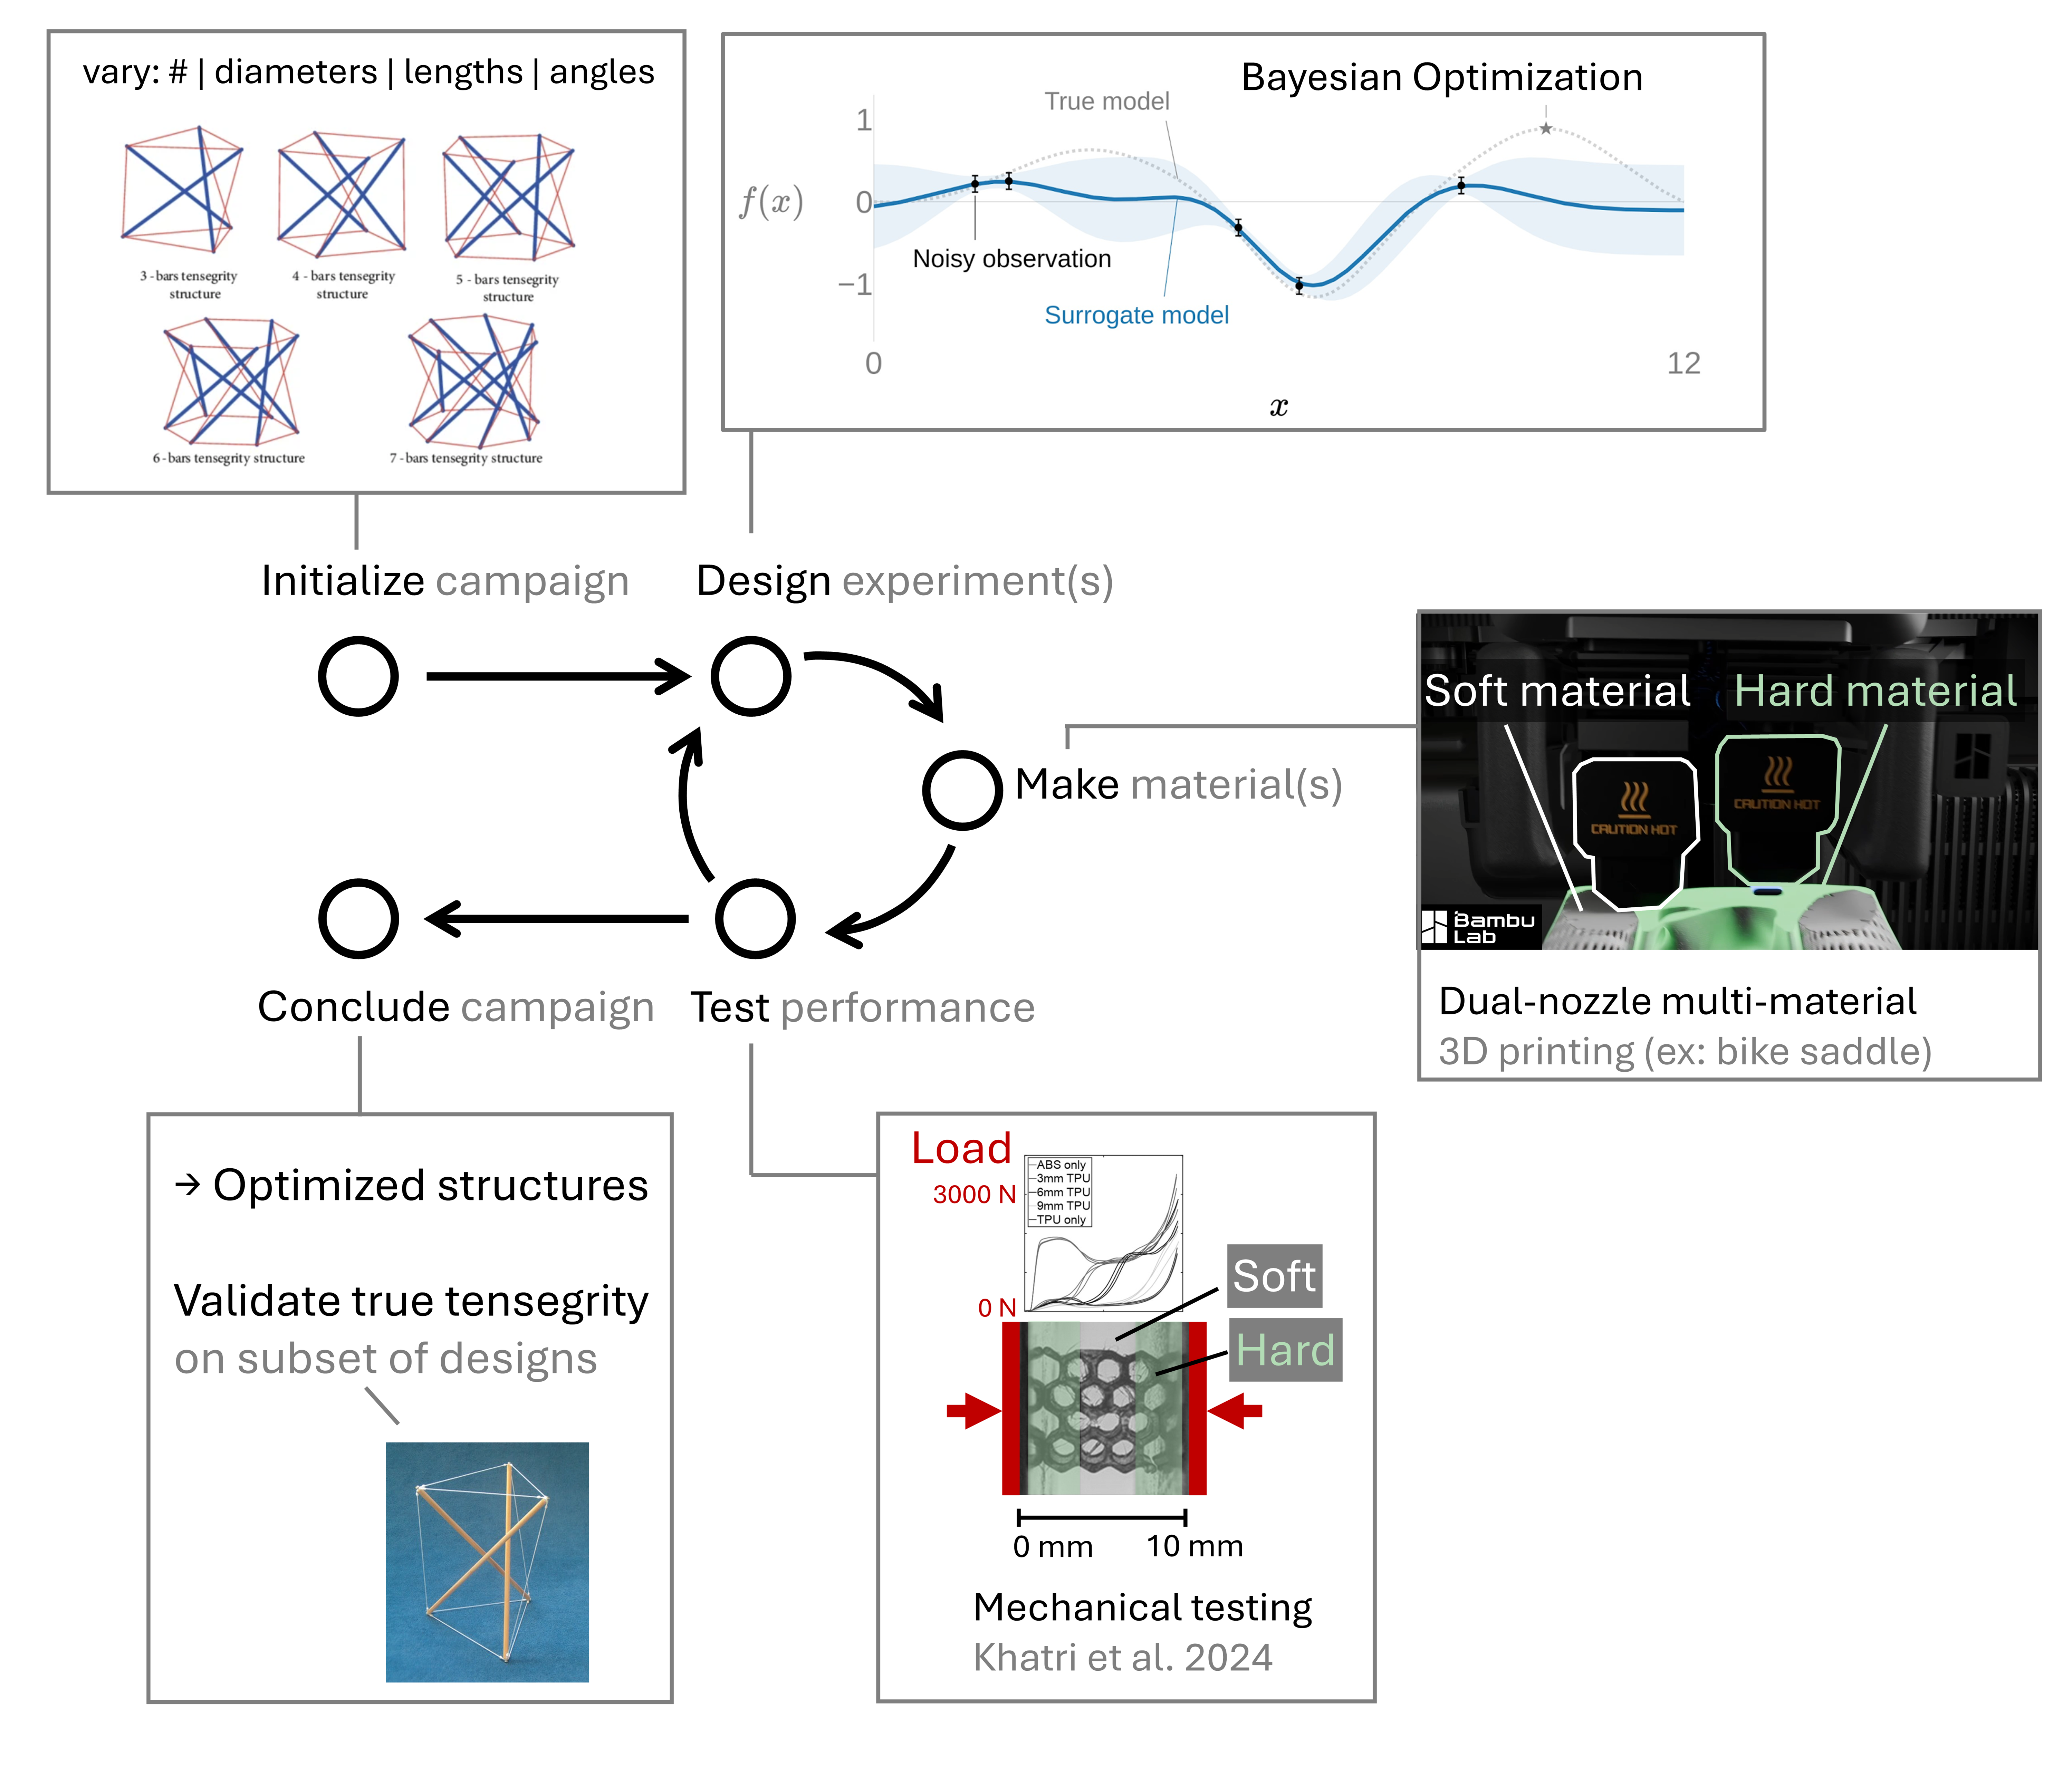
\includegraphics[width=0.7\textwidth]{../figures/overview-updated.png}
  \caption{Closed-loop, experiment-driven design framework. Parameterized
    PLA/TPU tensegrity-inspired unit cells are printed, characterized by
    repeated instrumented drop-weight impacts, and the resulting
    performance data drive a Gaussian-process surrogate that recommends the
    next batch of designs to fabricate.}
  \label{fig:overview}
\end{figure*}%
\todo{Eventually switch this overview figure to a vertical orientation; it is
  currently reproduced from the MRG proposal
  (\texttt{figures/overview-updated.png}).}

The remainder of the paper is organized as follows.
Section~\ref{sec:background} reviews tensegrity mechanics, multi-material
3D printing for energy absorption, and Bayesian optimization with an
emphasis on multi-objective and noise-robust acquisition functions.
Section~\ref{sec:methods} introduces the design parameterization,
fabrication workflow, drop-tower protocol and objectives, and BO loop,
and states the planned metal-analog comparison.
Section~\ref{sec:results} reports all four measured batches, the
surrogate audits, and the replication findings, and
Section~\ref{sec:discussion} discusses the
implications and limitations of the approach. Section~\ref{sec:conclusions}
concludes.

% =============================================================================
\section{Background}
\label{sec:background}
% =============================================================================

\subsection{Tensegrity-Inspired Architectures for Energy Absorption}

Tensegrity prisms and their planar extensions exhibit
softening-stiffening response under
compression~\citep{amendola2014experimental, zhang2018tensegrity,
fraternali2015tensegrity}, characteristics desirable for impact
mitigation because the structure can absorb a large fraction of the
input energy at a controlled, sub-injurious force plateau.
Santos~\cite{santos2023towardanovel} recently characterized a tensegrity
energy-dissipation metamaterial reporting equivalent viscous damping
on the order of $\sim$23\% with negligible residual strain per impact,
underscoring the suitability of tensegrity-inspired architectures for
repeated-impact use cases.
The space program literature documents large-scale tensegrity-inspired
absorbers for planetary landing~\citep{agogino2018superball,
caluwaerts2014superball, sabelhaus2015system, vespignani2018design,
deitrich2022titan} and a long history of crushable energy-absorbing
landing systems~\citep{cloutier1966landing, adams2004merairbag,
jackson2014honeycomb}. Pajunen et~al.~\cite{pajunen2019design} demonstrated that
truncated-tetrahedral tensegrity-inspired unit cells can be directly
3D-printed and exhibit load-limiting plateaus, motivating the present
focus on additively manufactured TPU/PLA composites.
More recent work on dynamically loaded additively-manufactured
energy-absorbing lattices~\cite{davami2019dynamicenergyabsorption}, together
with Intrigila et~al.'s bistable tensegrity-like unit cell for lattice
metamaterials~\cite{intrigila2022fabricationandexperimental} as the closest
published analog, confirms that this architecture class also responds favorably
under impact and quasi-static loading, although neither study employed
multi-material FDM or closed-loop design optimization.
Table~\ref{tab:novelty} situates the present work against selected
prior efforts spanning the three elements combined here (impact-tested
printed tensegrity-inspired structures, rigid-flexible fabrication,
and BO of architected materials), making explicit that, among the
studies reviewed, no single prior study combines a multi-material FDM
tensegrity-inspired architecture with an \emph{experiment}-driven
optimization loop.

\begin{table*}[t]
  \centering
  \caption{Positioning of this work against selected prior efforts
    spanning the elements combined here. The present campaign uses
    physical drop measurements of the transmissibility ($t_{180}$)
    and a mass-weighted rebound energy score ($E_{\mathrm{reb}}$)
    as its BO responses; it does not optimize specific energy
    absorption or crush energy.}
  \label{tab:novelty}
  \footnotesize
  \setlength{\tabcolsep}{4pt}
  \begin{tabular}{@{}llllll@{}}
    \toprule
    Study & Architecture & Fabrication & Optimization & Response optimized & Ground truth \\
    \midrule
    Pajunen et~al.\ 2019~\cite{pajunen2019design}
      & Truncated-tetrahedral & Single-material & None & n/a & Experiment \\
      & tensegrity-inspired & 3D print & (single condition) & & (drop impact) \\[2pt]
    Intrigila et~al.\ 2022~\cite{intrigila2022fabricationandexperimental}
      & Bistable tensegrity-like & Single-material & None & n/a & Experiment \\
      & lattice unit cell & 3D print & & & (quasi-static compr.) \\[2pt]
    Mo et~al.\ 2023~\cite{mo2023accelerated}
      & Architected lattices & n/a (simulation) & Multifidelity BO & Simulated response & Simulation \\
      & & & & metric & (+ sparse high-fid.) \\[2pt]
    Almeida 2025~\cite{almeida2025highstrainrate};
      & Tensegrity-inspired & Additive & None reported & n/a & Experiment \\
    \ \ Davami 2025~\cite{davami2025dynamicanalysis}
      & structures & manufacturing & & & (high-rate/dynamic) \\[2pt]
    Wang et~al.\ 2026~\cite{wang2026integrated}
      & Tensegrity-inspired & Integrated & None reported & n/a & Physical \\
      & rigid-flexible metamat. & dual-material & & & validation \\[2pt]
    \textbf{This work}
      & Tensegrity-inspired & Multi-material & Experiment-driven & $t_{180}$; provisional & Physical \\
      & $T_3$-prism cell (PLA/TPU) & FDM (PLA + TPU) & BO (SAASBO/qNEHVI) & $E_{\mathrm{reb}}$ & experiment \\
    \bottomrule
  \end{tabular}
\end{table*}


\subsection{Multi-Material 3D Printing of PLA/TPU Composites}

Multi-material rigid-soft FDM enables stiff/compliant combinations on a
single platform with tunable energy absorption, demonstrated for thick-panel
origami with PLA (or ABS/CFRP) panels and TPU hinges~\cite{ye2023multimaterial}
and for ABS-TPU honeycombs~\cite{khatri2024energy}. Neither study is itself a
tensegrity, but both establish the rigid-soft co-printing route we adopt. Ye
et~al.~\cite{ye2023multimaterial}
introduced a \emph{wrapping-based} strategy in which rigid cores are
encapsulated by continuous soft skins, reported to reduce interface
delamination under cyclic loading, something we take inspiration from in our
designs.
Beyond these rigid-soft demonstrations, a growing body of work confirms
that genuinely tensegrity-inspired architectures can be additively
manufactured and exhibit programmable mechanical response. Bauer
et~al.~\cite{bauer2021tensegrity} showed that 3D-printed tensegrity
metamaterials delocalize deformation to resist catastrophic failure, while
Pajunen et~al.~\cite{pajunen2021prestrain} tuned acoustic bandgaps in
3D-printed tensegrity-inspired lattices through prestrain, and
Sabouni-Zawadzka et~al.~\cite{sabounizawadzka2024experimental}
experimentally characterized 3D-printed tensegrity-inspired metamaterials
built on the simplex module. More directly relevant to impact, Almeida
et~al.~\cite{almeida2025highstrainrate} and Davami
et~al.~\cite{davami2025dynamicanalysis} characterized the high-strain-rate
and dynamic response of additively manufactured tensegrity-inspired
structures, and Wang et~al.~\cite{wang2026integrated} reported an
integrated fabrication-and-validation workflow for tensegrity-inspired
rigid-flexible metamaterials. Collectively these studies establish the
additive-manufacturability, tunability, and impact relevance of the
architecture class adopted here, none combining multi-material FDM with an
experiment-driven optimization loop.
Recent multi-material PLA/TPU sandwich and layered
composites~\citep{arifvianto2022mechanicalpropertiesof} report
quantitative bounds on
stiffness, strength, and energy absorption for the same PLA-TPU pair
used here, while FDM PLA fatigue
data~\citep{ezeh2018onthefatigue, vanaei2021multiscaledamageanalysis}
inform conservative design bounds for the rigid struts.
Architected multi-material lattices with co-printed compliant skins
have been explicitly designed for high specific energy
absorption~\citep{yavas2022designandfabrication}; recent surveys catalogue the
rapidly expanding additively manufactured polymeric energy-absorption
literature~\citep{bustihan2026recentadvancesin,
liu2026threedimensionalprintedlattice}. \todo{Add a short paragraph on
relevant TPU/PETG tensegrity search-space bounds once the Edison
literature task \texttt{5ae24eaf-5b6e-45cf-9f6c-1c7fbd881738}
synthesis is integrated.}

\subsection{Bayesian Optimization for Architected-Material Design}

Bayesian optimization is a sequential, model-based strategy for
optimizing expensive black-box functions using a Gaussian-process
surrogate~\citep{shahriari2016taking, frazier2018tutorial}. Modern
implementations such as BoTorch~\citep{balandat2020botorch} and the Ax
platform built atop it~\citep{pmlr-v293-olson25a} support
parallel batched evaluations and a wide variety of acquisition
functions; recent algorithmic advances include log-EI for numerical
robustness~\citep{ament2023logei}, noisy expected hypervolume
improvement for multi-objective settings~\citep{daulton2021nehvi},
input-noise-robust acquisitions~\citep{daulton2022robust}, and
evolution-guided constrained multi-objective BO for self-driving
labs~\citep{low2024evolution}. Mixed/categorical search spaces, needed
for the planned connectivity-topology extension rather than the
continuous $T_3$-prism prototype studied here, have dedicated
treatments in BOCS~\citep{baptista2018bocs} and the
one-hot-with-rounded-kernel construction
of~\citep{garridomerchan2020dealingwithcategorical}. BO has been
applied to architected-material
design~\citep{mo2023accelerated}
and to additive manufacturing~\citep{zhang2021bo}.
Mo et~al.~\cite{mo2023accelerated} in
particular established a multifidelity BO framework for architected
materials by fusing low-fidelity simulations with high-fidelity
ground truth via nonlinear information-fusion
priors~\citep{perdikaris2017nonlinear}; the present work shifts the
emphasis from simulation surrogates to direct experimental data,
appropriate for materials whose constitutive response is difficult to
calibrate from first principles.

% =============================================================================
\section{Materials and Methods}
\label{sec:methods}
% =============================================================================

\subsection{Design Parameterization}
\label{sec:methods:parameterization}

We parameterize a family of tensegrity-inspired unit cells via four
groups of design variables. For the working $T_3$-prism prototype that
defines the initial BO search space (Section~\ref{sec:methods:bo}),
only the first two groups are active and all of their variables are
\emph{continuous}; the connectivity-topology and tiling groups are
held fixed for this prototype and are listed here as planned
extensions of the design family:
\begin{itemize}
  \item \textbf{PLA compression members.} Strut diameter $d_s$ and
    length $\ell_s$, with the slenderness ratio $\ell_s / d_s$ bounded
    away from buckling-dominated regimes.
  \item \textbf{TPU tension elements.} Cross-sectional area $A_t$ (or
    equivalent diameter $d_t$ for circular cross-sections).
  \item \textbf{Connectivity topology (future extension).} Selected
    from a discrete set of candidate unit cells (e.g.,
    truncated-tetrahedral, prism-based, and octahedral variants); when
    activated, the design vector would encode this as a categorical
    choice. It is held fixed at the $T_3$ prism for the present
    campaign.
  \item \textbf{Unit-cell tiling (future extension).} Number of cells
    $N_x \times N_y \times N_z$ and the orientation of each cell
    relative to the impact direction; held fixed at a single cell here.
\end{itemize}
\todo{Specify exact manufacturing-feasibility constraints once
finalized; the connectivity-topology categorical encoding is deferred
until that variable is activated beyond the $T_3$ prism.}

\paragraph{Working prototype and search-space evolution} The first
instance of this family used to validate the fabrication and test
pipeline is a three-strut, $T_3$-prism-inspired cell scaled to a
$\sim$50\,mm bounding box. In batches 1 and 2 the BO harness exposes
five continuous design variables (base radius $R$, cell height $H$,
twist angle $\theta$, a single strut diameter $d_s$, and a single
cable (tendon) diameter $d_t$) over the ranges listed in
Table~\ref{tab:design-vars}; the cable diameter $d_t$ is treated as a
\emph{continuous} variable on $[3.0, 5.5]$\,\si{mm} rather than a
discrete set. From batch 3 the space grows to include the print
process: two per-article sparse-infill densities (strut and tendon,
each 12 to 35\%) chosen by the acquisition for every article, and
four filament settings (PLA and TPU nozzle temperature and maximum
volumetric speed) that are physically one value per print job, so
they are drawn as one quasi-random point per batch and are
acknowledged as confounded with batch until a round varies them
within a plate (Section~\ref{sec:methods:bo}). Under the prism's
$D_3$ symmetry all struts share one diameter and all cables share one
diameter, so the parameterization uses a single strut-diameter axis
and a single cable-diameter axis (two member-diameter axes), leaving
room to relax to per-orbit (saddle, top, bottom) or fully per-member
diameters once the individual orbits have been characterized.\todo{Cite the
heterogeneous-parameters Edison LITERATURE\_HIGH brief
(\texttt{5191cf4d}) on $D_3$-symmetric vs.\ fully-per-member
parameterization.} The joint diameter $d_j$ is held fixed at
\SI{7.0}{mm} rather than optimized: it sets the printed strut-end cage
that houses the internal cable anchors
(Section~\ref{sec:methods:fabrication}), so it is constrained primarily by the
TPU-tendon outlet count and the dual-nozzle clearance rather than by
energy-absorption performance, and fixing it keeps the anchor geometry
constant across specimens so that the optimized variables are not
confounded by joint-strength changes; relaxing $d_j$ is deferred to a
follow-on joint-design study. Figure~\ref{fig:printed-prototypes}
shows the parametric CAD model alongside an as-printed prototype of this
working $T_3$ prism.

\paragraph{Constant-mass projection and printability screens} Because
cell mass varies severalfold across the raw design box, an
unconstrained search would partly reward designs for carrying more
material rather than for their architecture. Every candidate is
therefore projected onto a constant material budget before printing:
the design is uniformly rescaled (all dimensions except the twist
angle) until its mass target is met, converged to within
\SI{0.15}{g} on rendered geometry. The target evolved with the
campaign. Batches 1 and 2 held \emph{solid} CAD mass
$\rho_{\mathrm{PLA}} V_{\mathrm{PLA}} + \rho_{\mathrm{TPU}}
V_{\mathrm{TPU}}$ at $m^{\star} = \SI{30.95}{g}$, the solid mass of
the reference prism. That budget does not hold printed grams
constant, because PLA struts print at partial infill while thin TPU
cables print near solid: as-printed masses spanned
\SIrange{18.50}{22.04}{g} across the tested seed articles
(coefficient of variation 5.5\%) and \SIrange{17.91}{23.47}{g}
(8.7\%) across batch 2, so the abstract's ``common mass budget'' is
approximate for those batches and the surrogate carries each
article's weighed mass explicitly
(Section~\ref{sec:methods:bo}). From batch 3 the projection instead
holds \emph{printed} mass at \SI{20.23}{g} (the reference article's
weight) by inverting the calibrated printed-mass model described in
the Supplementary Information; the achieved batch mass CVs were
1.7\% (batch 3) and 2.3\% (batch 4). Two printability screens are
evaluated on the projected geometry and recorded as flags rather
than hard rejections: a cylindrical build envelope
$\pi R^2 H \le \SI{250}{cm^3}$ and the \SI{3.0}{mm} TPU
self-bridging floor on the as-projected cable diameter (the
projection can scale a nominally feasible cable below the floor; the
two seed designs where this occurred both exhibited tendon stringing
defects, consistent with the screen, and the batch-4 attenuators
printed at 2.5 to \SI{2.8}{mm} with only minor stringing, so the
floor is a defect predictor rather than a hard failure line).

\begin{table}[ht]
  \centering
  \caption{Design variables for the $T_3$-prism campaign, as implemented
    in the BO harness. The seed batch is an $n=9$ Sobol draw (fixed
    seed) over the five geometry variables, with each design then
    projected onto the constant-mass budget of the text. The process
    variables joined the space in batch 3: the two infill densities
    are acquisition-chosen per article, while the four filament
    settings admit one value per print job and are therefore drawn as
    a single quasi-random point per batch (confounded with batch
    until varied within a plate). The joint diameter is held fixed.
    All specimens print in the vertical orientation on a Bambu
    Lab~H2D: one specimen per named build plate in the seed batch,
    one nine-article plate per batch thereafter.}
  \label{tab:design-vars}
  \small
  \begin{tabular}{@{}llccc@{}}
    \toprule
    Variable & Symbol & Units & Range & Active \\
    \midrule
    Base radius            & $R$       & mm  & 25-40 & batch 1 on \\
    Cell height            & $H$       & mm  & 60-110 & batch 1 on \\
    Twist angle            & $\theta$  & deg & 40-80 & batch 1 on \\
    Strut (PLA) diameter   & $d_s$     & mm  & 6.0-12.0 & batch 1 on \\
    Cable (TPU) diameter   & $d_t$     & mm  & 3.0-5.5 & batch 1 on \\
    Strut infill density   & -        & \%  & 12-35 & batch 3 on \\
    Tendon infill density  & -        & \%  & 12-35 & batch 3 on \\
    PLA nozzle temperature & -        & \si{\celsius} & 212-228 & batch 3 on\textsuperscript{a} \\
    PLA volumetric speed   & -        & \si{mm^3/s} & 20-30 & batch 3 on\textsuperscript{a} \\
    TPU nozzle temperature & -        & \si{\celsius} & 235-245 & batch 3 on\textsuperscript{a} \\
    TPU volumetric speed   & -        & \si{mm^3/s} & 2.2-3.6 & batch 3 on\textsuperscript{a} \\
    Joint diameter (fixed) & $d_j$     & mm  & 7.0 & - \\
    \bottomrule
  \end{tabular}\\[2pt]
  {\footnotesize \textsuperscript{a}One value per print job (a plate
  carries a single filament configuration), so per-batch rather than
  per-article.}
\end{table}%
\todo{The cable-diameter lower bound (3.0\,mm) is set by the Bambu
  auto-support detection floor; add the remaining
  manufacturing-feasibility constraints once finalized.}

\paragraph{As-built resolution of the continuous variables} Although
$d_s$ and $d_t$ are treated as continuous, the as-built cross-sections
are discretized by the nozzle diameter, the slicer line width, and
support interaction, so the effective search granularity is coarser
than the nominal continuous box. The realized member diameter therefore
changes in steps set by the line-width quantization rather than
continuously, and the smallest CAD change that yields a reliably
distinguishable as-built member is bounded below by these slicer
limits; the lower TPU-tendon bound (\SI{3.0}{mm}) is itself a
workflow-specific limit tied to the TPU self-bridging and auto-support
detection floor on this H2D platform rather than a fundamental
geometric one. The as-built quantity measured for every article is its
mass, weighed on a \SI{0.01}{g} scale; dimensional metrology of the
printed members has not yet been performed, so the geometry attached
to the surrogate is the commanded post-projection geometry. Two
print-to-print measurements bound the fabrication scatter: one seed
design printed in triplicate has a mass standard deviation of
\SI{0.457}{g}, and the full reprint of the batch-3 plate produced
nine design-replicate mass pairs whose second print weighed
\SI{0.27}{g} heavier article for article on average, a per-session
flow offset rather than random scatter. Both feed the observation
noise model (Section~\ref{sec:methods:bo}).

\begin{figure}[t]
  \centering
  \begin{subfigure}[b]{0.42\linewidth}
    \centering
    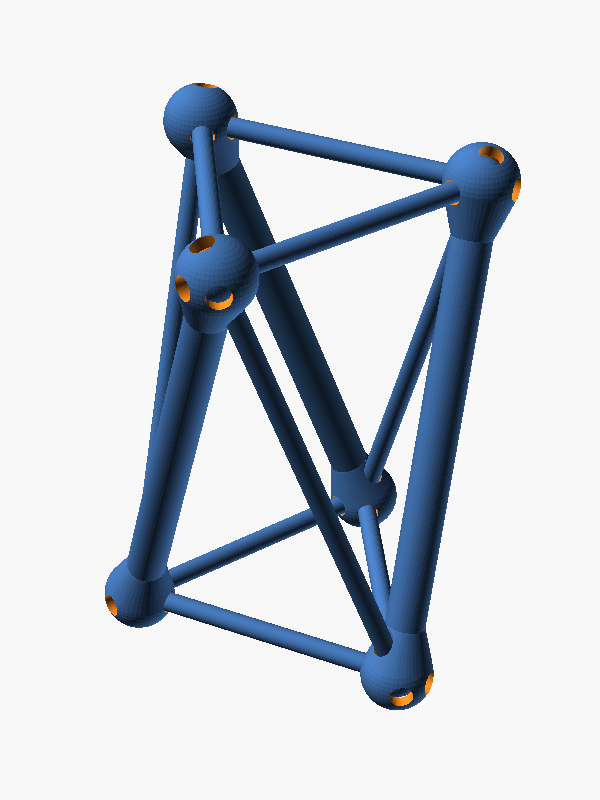
\includegraphics[width=\linewidth]{../figures/photos/cad-render.png}
    \label{fig:proto-cad}
  \end{subfigure}\hfill
  \begin{subfigure}[b]{0.54\linewidth}
    \centering
    \begin{tikzpicture}
      \node[anchor=south west,inner sep=0] (ph)
        {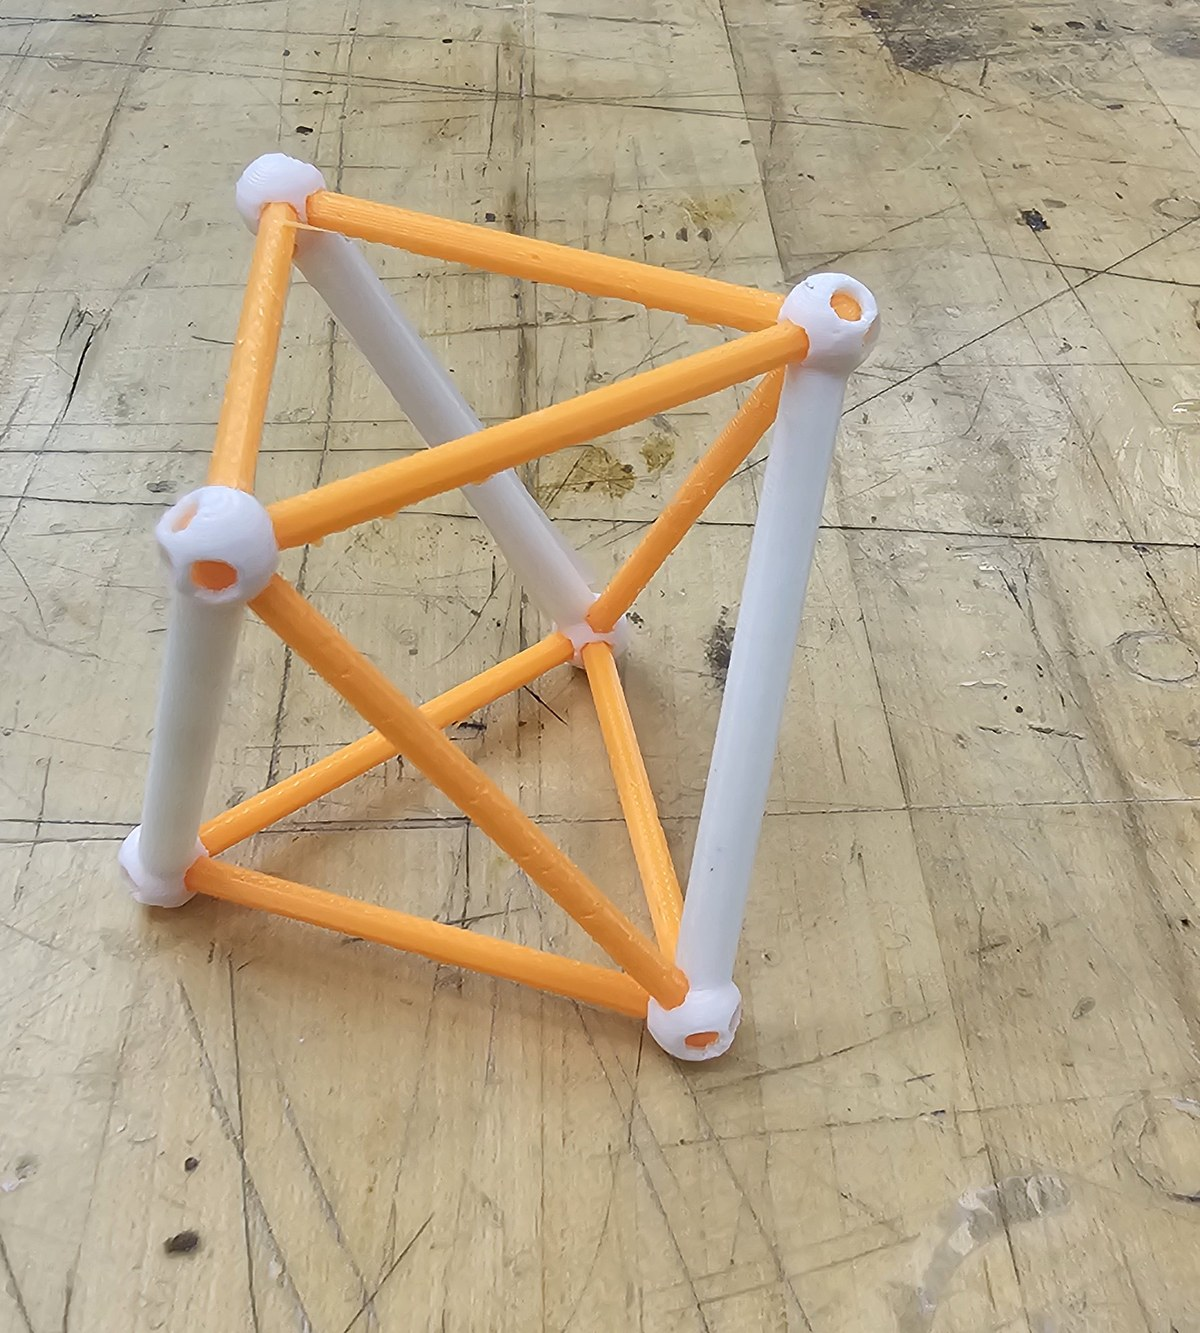
\includegraphics[width=\linewidth]{../figures/photos/printed-specimen.jpg}};
      \begin{scope}[x={(ph.south east)},y={(ph.north west)},
                    font=\sffamily\scriptsize]
        \tikzset{callout/.style={-{Latex[length=1.5mm]},line width=0.5pt,
                                 draw=red!75!black}}
        \tikzset{lab/.style={fill=white,fill opacity=0.85,text opacity=1,
                             inner sep=1pt,rounded corners=1pt}}
        \draw[callout] (0.74,0.95) node[lab,anchor=south]{$d_s$}
          -- (0.63,0.52);
        \draw[callout] (0.22,0.96) node[lab,anchor=south]{$d_t$}
          -- (0.34,0.70);
        \draw[{Latex[length=1.5mm]}-{Latex[length=1.5mm]},line width=0.5pt]
          (0.05,0.23) -- (0.05,0.85) node[lab,midway]{$H$};
      \end{scope}
    \end{tikzpicture}
    \label{fig:proto-print}
  \end{subfigure}
  \caption{Working $T_3$-prism prototype. \emph{(a)} Parametric OpenSCAD model
    whose base radius $R$, cell height $H$, twist angle $\theta$, strut diameter
    $d_s$, and cable diameter $d_t$ are the design variables of
    Table~\ref{tab:design-vars}. \emph{(b)} A representative dual-material print
    from the PR~\#35 print history (rigid PLA struts, here in white; tendon
    members in orange), with callouts marking the strut diameter $d_s$, a tendon
    (cable) diameter $d_t$, and the cell height $H$; the inter-plate twist
    $\theta$ is the relative rotation of the top and bottom node triangles, and
    the base radius $R$ sets their circumradius.}
  \label{fig:printed-prototypes}
\end{figure}

\subsection{Multi-Material Fabrication}
\label{sec:methods:fabrication}

Specimens are fabricated on a multi-material FDM printer using PLA for
the rigid struts and TPU for the soft tension elements.
Figure~\ref{fig:fab-workflow} summarizes the end-to-end fabrication and
characterization workflow, from parametric CAD through multi-material
slicing, dual-extrusion printing, post-processing, and mechanical
testing. Rather than
wrapping the struts in a continuous TPU skin, the current design anchors
the TPU tension elements \emph{inside} the ends of each PLA strut: the
cables converging at a given strut end are joined within the strut,
which acts as a rigid cage housing the junction, and the individual
tendons then exit through discrete outlets. This keeps the soft-rigid
interface in internal, compression-dominated pockets rather than at an
exposed overmolded surface. This construction effectively inverts the
material roles of Ye et~al.'s soft-skin-over-rigid-core
wrapping~\cite{ye2023multimaterial}: here a soft TPU core is captured within
a rigid PLA shell, so we cite that work only as a multi-material co-printing
precedent rather than as validation of the present junction. \todo{Quantitatively
verify the internal-anchoring junction strength against the PR~\#39 / PR~\#35
joint pull-out studies before making any cyclic-durability claim.} \todo{Document slicer profile
(layer height, infill, print speed, nozzle temperatures, retraction
settings) and validation prints used to characterize PLA-TPU interface
strength.}

\paragraph{Print platform and joint geometry} The working platform is
a Bambu Lab~H2D printer, which permits a single rigid-soft build
without filament swaps. Strut endpoints are tied to cables through
parametric joint geometries developed and ranked through a five-design
OpenSCAD study (anchor-bulb, dovetail, TPU-sleeve overmold,
eyelet-loop, and TPU-rebar variants); the working prototype uses a
dovetail joint (Design~B) with an anchor-bulb backup (Design~A) for
sensitivity studies, with a captive TPU core routed inside the PLA
shell to keep the soft tendon protected from layer-line failure at
the strut-to-cable transition. The full five-design comparison and the
selected junction are detailed in the Supplementary Information.\todo{Cite the
joint-design Phase-3 CAD review (Edison ANALYSIS \texttt{19e0c868}) and the
Phase-4 vision review (\texttt{e9a1f4cc}) once both are integrated into the
references.}

\paragraph{Supports for soft members} Because near-vertical TPU
tendons are otherwise unsupported during printing, automatic support
generation is disabled and supports are painted manually in the
slicer: PLA edge supports run along each tendon, with the
support-to-object clearance tightened from \SI{0.35}{mm} to
\SI{0.2}{mm} during tuning on the reference prism. Two support-removal
artifacts recur in the seed batch (surface stringing and, on two
articles, TPU strands pulled off bottom tendons during support
removal) and are logged per article in the print key (Supplementary
Information). An automated alternative (a lowered support-threshold
angle plus mesh-ray-cast narrowing pillars) was developed in parallel
and is documented in the Supplementary Information.

\paragraph{Moisture and nozzle management} TPU is hygroscopic, so the
soft filament is fed from a heated dry box held near \SI{8}{\percent}
relative humidity, logged per print. Midway through the seed batch the
TPU extruder developed a progressive flow taper (a partial clog,
compounded by a stray PLA fragment found inside the extruder); it was
resolved by a cold pull and by moving the TPU to a dedicated
high-flow \SI{0.6}{mm} nozzle, after which print quality was restored.
The affected and post-fix articles are identified in the print key so
that any nozzle-related covariate can be checked against the measured
objectives.

\begin{table}[ht]
  \centering
  \caption{Multi-material print parameters on the Bambu Lab~H2D,
    transcribed from the archived as-printed Bambu Studio project
    (\texttt{t3-prism-bo-batch.H2D-MM-PLAstruts-TPUcables.as-printed.3mf},
    Bambu Studio 2.7.1). Filaments are Bambu Lab PLA Basic (struts,
    support material) and Bambu Lab TPU~85A (tendons); the print
    profile is ``0.30\,mm Standard @BBL H2D 0.6 nozzle.'' The
    reporting structure follows the methods section of Ye
    et~al.~\cite{ye2023multimaterial}.}
  \label{tab:print-params}
  \small
  \setlength{\tabcolsep}{3pt}
  \begin{tabular}{@{}lcc@{}}
    \toprule
    Parameter & PLA (struts) & TPU 85A (tendons) \\
    \midrule
    Nozzle                             & \SI{0.6}{mm} & 0.4 then \SI{0.6}{mm} HF\textsuperscript{a} \\
    Nozzle temperature (\textdegree C) & 220 & 220 \\
    Bed temperature, profile (\textdegree C) & 55 & 35 \\
    Layer height / line width (mm)     & \multicolumn{2}{c}{0.30 / 0.62} \\
    Infill                             & 15\% grid, 2 walls & near-solid \\
    Outer / inner wall speed (mm/s)    & \multicolumn{2}{c}{200 / 300 (profile)} \\
    Filament drying                    & n/a & dry box, $\sim$8\% RH \\
    Build-plate type                   & \multicolumn{2}{c}{Textured PEI} \\
    Build orientation                  & \multicolumn{2}{c}{Vertical} \\
    Supports                           & \multicolumn{2}{c}{Manual painted tree supports, PLA} \\
    \bottomrule
  \end{tabular}\\[2pt]
  {\footnotesize \textsuperscript{a}The TPU side ran a standard
  \SI{0.4}{mm} nozzle until the mid-batch clog, then a dedicated
  high-flow (HF) \SI{0.6}{mm} nozzle; affected articles are flagged in
  the print key.}
\end{table}%
\todo{@achris0520 to confirm the physical nozzle hardware (the
  archived as-printed project records \SI{0.6}{mm} on both extruders,
  consistent with the post-fix state; the TPU side ran \SI{0.4}{mm}
  before the mid-batch nozzle change logged in the print key) and to
  supply filament lot numbers and drying duration, which the slicer
  archive does not record.}

\begin{figure*}[t]
  \centering
  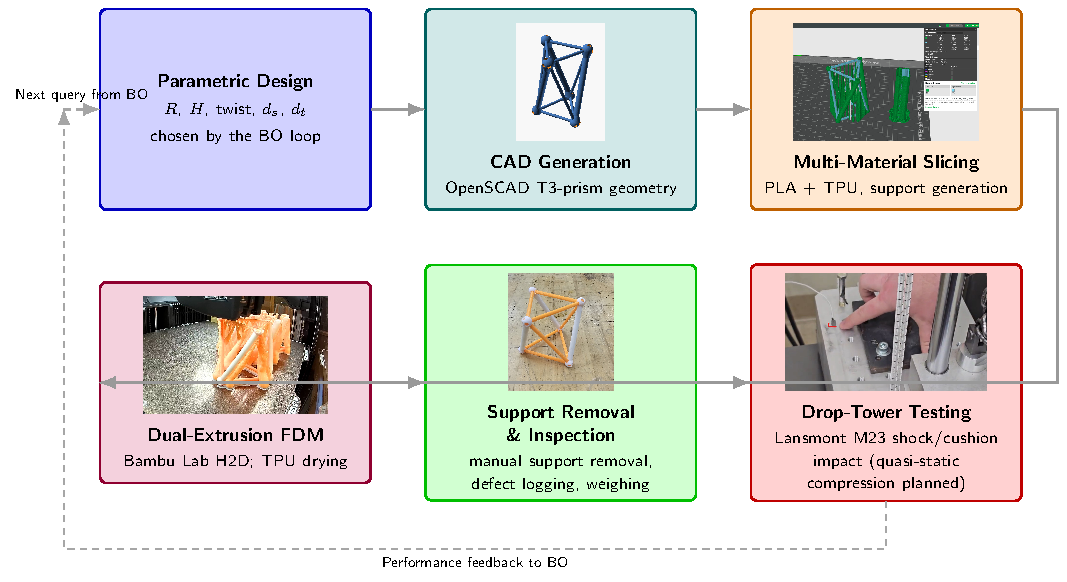
\includegraphics[width=\textwidth]{../figures/fab-workflow.pdf}
  \caption{Fabrication and characterization workflow for the multi-material
    tensegrity-inspired unit cells: design parameters drive parametric CAD,
    slicing with manually generated TPU supports, a single multi-material
    print on the Bambu Lab~H2D, post-processing and inspection, and
    mechanical testing. Node photographs are representative artifacts drawn
    from the project's build history: the OpenSCAD $T_3$-prism render
    (CAD), the dual-nozzle Bambu Studio slice with PLA on the left extruder
    and TPU on the right (slicing), an in-progress H2D print of the prism
    batch (FDM), an as-printed specimen (post-processing), and the
    bungee-assisted drop-tower base plate with accelerometer (testing).}
  \label{fig:fab-workflow}
\end{figure*}%

\subsection{Experimental Characterization}
\label{sec:methods:testing}

\paragraph{Drop-tower fixture} The primary characterization is
repeated drop-weight impact on a Lansmont Model~23 shock test system.
The printed specimen rides upright on the carriage plate, which is
raised \SI{60}{in} (\SI{1.524}{m}) along guide rails and released; the
plate lands on a single \SI{0.5}{in} Shore 60~OO polyurethane cushioning
sheet, which shapes the landing into a single sharp base pulse of
roughly \SI{1.6}{ms} duration. This impact-surface configuration was
selected by a blinded crossover experiment over three candidate mat
arrangements, and unlike a felt stack it does not measurably compact
over hundred-drop sessions. Rig health is monitored continuously
through the impact velocity change $\Delta v$ recovered from the base
accelerometer: over an uninterrupted 100-drop characterization session
the $\Delta v$ coefficient of variation was 0.54\% with no drift, and
every campaign session is checked against the healthy tower baseline
(details, including the within-session mat warm-up and recovery
pattern, in the Supplementary Information). One drop takes roughly
\SI{42}{s}, so a seed-batch characterization completes in about
ninety minutes per article and a later-batch session in about
fifteen.

\paragraph{Instrumentation and signal processing} A single-axis
piezoelectric accelerometer on the carriage plate records the base
input and triggers the acquisition; a triaxial accelerometer (Dytran
3133A4) seated in a printed pocket at the specimen's top vertex records
the transmitted response. The two base-capable channels were
cross-calibrated in place over fifteen co-located drops (ratio
$0.953 \pm 0.001$ at matched filtering), and the transducer settings
are archived with the data. Signals are captured at
\SI{1.25}{MHz} over a \SI{100}{ms} record with a \SI{2}{ms}
pre-trigger. All channels are low-pass filtered with the SAE~J211/1
channel-frequency-class (CFC) filters~\citep{saej211}, implemented from
the standard's published coefficients with the two-pass corner
frequency handled explicitly (a common implementation shortcut narrows
the passband by roughly 20\%, which we identified and corrected before
the campaign; all reported numbers use the corrected filter). CFC-180
is the reporting class for peak metrics, with CFC-1000 retained as a
higher-bandwidth diagnostic.

\paragraph{Per-article objectives and session protocol} Session
length evolved with the campaign's understanding of its own noise,
and the per-batch counts are stated here because they differ. Seed
sessions recorded 103 drops per article and contribute 101 stabilized
captures each (103 for one article, autv5r) after the first two drops
of each session are discarded as seating warm-up. A pre-campaign
variance study on the commissioning datasets put the statistical
minimum at five stabilized drops after two warm-ups, and the seed
sessions confirmed that the stabilized mean is insensitive to session
length: within-session per-drop CVs of 0.17 to 0.48\% with flat
post-warm-up trends, and a replay of the seed sessions truncated to
twenty drops leaves the transmissibility ranking of all eight tested
articles unchanged, with a worst-case mean shift of $+0.008$ against
design-to-design gaps of 0.007 to 0.087 and a per-drop standard
error still an order of magnitude below those gaps. Later sessions
were therefore shortened to about twenty drops per article: the
committed record lists 21 to 22 valid captures per batch-2 article
and 20 recorded drops per article in batches 3 and 4, against 101
valid captures per seed article, with the first two drops of every
session discarded as before (exact per-session counts are in the
archived per-drop records). The shortening cuts tower time per
article
from about ninety minutes to about fifteen while retaining roughly
four times the minimum stabilized-drop budget; a shorter session
simply enters the surrogate with a proportionally larger standard
error, which the model downweights. The second print-and-test pass
of batch 3
(Section~\ref{sec:results:batches}) subsequently confirmed that
seating and print variation, not session length, limit what a
session can claim, so the freed tower time goes to re-seats. Each
session yields two objectives, each reported as a stabilized mean
with the per-drop scatter quoted as one standard deviation; the
standard error of the mean is what enters the surrogate's noise model
(Section~\ref{sec:methods:bo}):
\begin{equation}
  \begin{aligned}
    t_{180} &\;=\; \frac{\max_t\,\lVert \mathbf{a}_{\mathrm{top}}(t)\rVert_{\mathrm{CFC180}}}
                        {\max_t\,\lvert a_{\mathrm{base}}(t)\rvert_{\mathrm{CFC180}}},\\
    E_{\mathrm{reb}} &\;=\; e_{\mathrm{reb}}\, m\, g\, h,
    \qquad
    e_{\mathrm{reb}} \;=\; \frac{g\, t_{\mathrm{second}}}{2\,\Delta v},
  \end{aligned}
  \label{eq:objectives}
\end{equation}
where $t_{180}$ is the CFC-180 filtered peak-acceleration ratio,
which we name once here and then call the \emph{transmissibility}
throughout: the peak magnitude of the triaxial top-vertex response
over the peak base input within the impact window. The term is used
in the shock-testing sense standard for cushioning and packaging
drop tests, a ratio of filtered peak accelerations across the
article under a single transient, not the steady-state
frequency-response function of vibration isolation: the two peaks
need not be simultaneous, the filter class is part of the
definition, and SAE~J211/1 is cited only for the impact-channel
filtering. Values above unity indicate the structure amplifies the
peak shock reaching its top vertex; values below unity indicate
attenuation. $E_{\mathrm{reb}}$ is a \emph{provisional
mass-weighted rebound score} with units of energy (millijoules per
drop): the dimensionless rebound fraction $e_{\mathrm{reb}}$ is
recovered from the ballistic timing of the top vertex's post-impact
hop~\citep{bernstein1977listening} ($t_{\mathrm{second}}$ is the time
to the second contact event and $\Delta v$ the measured base velocity
change), and it is scaled by each article's own weighed mass $m$ and
the drop height $h$. Two interpretive caveats are deliberate. The
ballistic reading of the second contact event has not yet been
validated against synchronized video, and $\Delta v$ is the base
plate's velocity change rather than a demonstrated incident relative
velocity, so $e_{\mathrm{reb}}$ is a rebound-timing score rather than
a coefficient of restitution; and because a strict restitution reading
would scale returned kinetic energy as the \emph{square} of a velocity
ratio, $E_{\mathrm{reb}}$ is a mass-aware ranking score that penalizes
designs (and grams) that throw more motion back at the payload, not a
measured rebound energy. The score is the campaign's second
objective through all four batches and remains a candidate to become
a constraint once validated
(Section~\ref{sec:discussion}). Using the mass-weighted form rather
than the bare fraction keeps the objective mass-aware: equal fractions
on articles of different printed mass are not equivalent outcomes for
a payload. Ringdown descriptors (the fitted natural frequency $f_n$,
260 to \SI{470}{Hz} for every article but one batch-4 design that
rings at \SI{764}{Hz}, and, where
the exponential fit passes an $r^2 \ge 0.85$ gate, a damping ratio
$\zeta$) are recorded per drop as print-health and prestress
diagnostics~\citep{ashwear2014natural} but are not campaign objectives.
The within-session per-drop CV of $t_{180}$ spans 0.06 to 2.0\%
across the campaign's 35 articles (0.17 to 0.48\% in the seed
batch). These
values describe repeated drops of the same physical article in one
seating and do not estimate print-to-print or seating-to-seating
repeatability; serial dependence among drops may also make
$s/\sqrt{n_{\mathrm{drops}}}$ optimistic. Two replication
measurements bound what a single session can claim: the seed
attenuator re-measured across a day and an independent re-seat
agreed to 0.13\%, while a full second print-and-test pass of the
batch-3 plate showed same-design shifts with a median of $+1.2\%$
and heavy tails (Section~\ref{sec:results:batches}). The campaign
therefore adopted a between-seat replication rule: a single-seating
value that would drive a decision (a batch extreme, a claimed
attenuator, a front membership) requires confirmation on an
independent re-seat before it is treated as a design property. A
mechanism-oriented trace figure (processed
deceleration response with event markers keyed to synchronized video
frames) will be generated from archived campaign captures once the
event labels can be supported by synchronized measurements; no such
figure is shown here because none of the required event
synchronization has yet been performed.

\paragraph{Planned quasi-static extension} The drop test loads the
specimens in their elastic regime (the crush lasts 1 to \SI{3}{ms} and
the article recovers), so crush-energy metrics such as specific energy
absorption (SEA) and compaction efficiency are not recoverable from
these captures by any reprocessing. A quasi-static compression
campaign on a benchtop load frame (BYU CB~123 Instron, with a
low-range load cell appropriate to the expected cell stiffness)
is planned to supply the complementary crush metrics
\begin{equation}
  \mathrm{SEA} \;=\; \frac{1}{m}\!\int_{0}^{\delta_d}\! F(\delta)\,
  \mathrm{d}\delta,
  \qquad
  \eta_c \;=\; \frac{\int_{0}^{\delta_d}\! F(\delta)\,\mathrm{d}\delta}{F_{\max}\,\delta_d},
\end{equation}
with the densification displacement $\delta_d$ taken at the maximum of
the energy-absorption efficiency curve and $F_{\max}$ the peak force
within $[0,\delta_d]$, following the canonical cellular-solid
treatments~\citep{gibson1997cellular, avalle2001characterization,
tan2005dynamic, michailidis2011establishment} and mirroring the
quasi-static protocol of Pajunen et~al.~\citep{pajunen2019design}.
These metrics are reported as a complementary characterization of
selected designs rather than as objectives of the drop-tower campaign.
Slip resistance and traction at the specimen-to-floor interface,
governed by the tip geometry rather than the internal architecture,
follow ISO 11334-4~\citep{iso11334-4} for walking-aid tips and are out
of scope for the present axial-impact study.

\paragraph{Complementary data streams} High-speed video
(\SI{959}{fps}, three clips per specimen) supplements the
accelerometer data. The camera cannot resolve the millisecond-scale
impact pulse (one to two frames), so the division of labor is
explicit: the accelerometer channels produce the objectives, and video
documents the post-impact rebound and recovery. Synchronized
laser-Doppler vibrometry is reserved for follow-up characterization of
selected designs.

\subsection{Experiment-Driven Bayesian Optimization Loop}
\label{sec:methods:bo}

The optimization loop maintains a Gaussian-process (GP) surrogate over
the design space defined in
Section~\ref{sec:methods:parameterization}. After each round of
physical experiments, the surrogate is refit and an acquisition
function is maximized to recommend the next batch of designs to
fabricate. The campaign is posed as a two-objective minimization:
simultaneously minimize the transmissibility $t_{180}$
and the per-drop rebound energy $E_{\mathrm{reb}}$ of
Eq.~\eqref{eq:objectives}. Both objectives serve the same payload:
$t_{180}$ bounds the peak shock it feels during the impact, and
$E_{\mathrm{reb}}$ penalizes the motion thrown back into it afterward.
The seed data showed an apparent trade-off driven substantially by
the single strongest attenuator, not statistically resolved at seven
mapped articles (Spearman $\rho = -0.39$, $p = 0.38$;
Section~\ref{sec:discussion}); the measured front after four batches
is nondegenerate (its members span both axes), and the rebound axis
remains a candidate to become a constraint once its ballistic
reading is validated.
Implementation
uses the Ax platform~\citep{pmlr-v293-olson25a} over
BoTorch~\citep{balandat2020botorch}, with noisy expected hypervolume
improvement (qNEHVI)~\citep{daulton2021nehvi} as the multi-objective
acquisition. The $T_3$-prism search space is fully continuous,
including the process variables added in batch 3
(Table~\ref{tab:design-vars}), so no categorical
encoding is required; the mixed-search-space constructions
of~\citep{garridomerchan2020dealingwithcategorical} and the BOCS
combinatorial baseline~\citep{baptista2018bocs} remain the route for
the future connectivity-topology categorical rather than part of the
current loop. The input-noise-robust acquisition of Daulton
et~al.~\cite{daulton2022robust} and the evolution-guided constrained
variant of Low et~al.~\cite{low2024evolution} are held in reserve as
contingencies.

\paragraph{Surrogate and noise model} The surrogate is the fully
Bayesian sparse axis-aligned subspace model
(SAASBO)~\citep{eriksson2021saasbo}: a Mat\'ern-5/2 kernel with
automatic relevance determination whose length scales carry strong
sparsity-inducing priors and are marginalized by Markov-chain Monte
Carlo (NUTS) rather than point-estimated; every refit in the
campaign, through the batch-4 ingestion, uses this model with qNEHVI
on top (Ax 0.4 for the early rounds, Ax~0.5.0 from the batch-3
refit). We retain SAASBO even though the
dimensionality is modest because marginalizing the hyperparameters
tends to improve uncertainty quantification at the very small sample
sizes of physical campaigns; the fitted model is audited each round
with leave-one-out cross-validation and length-scale-based
sensitivity diagnostics
(Section~\ref{sec:results}). Inputs are normalized to the unit cube
and outputs standardized. Observation noise is supplied per
observation as a fixed variance: for $t_{180}$ the squared standard
error of the stabilized mean,
$\sigma_t^2 = s_{\mathrm{drop}}^2 / n_{\mathrm{drops}}$, and for the
rebound score the drop-scatter term plus the propagated
print-to-print mass scatter,
$\sigma_E^2 = \sigma_{E,\mathrm{drops}}^2 +
(\partial E_{\mathrm{reb}}/\partial m)^2 \sigma_m^2$ with
$\sigma_m = \SI{0.457}{g}$ measured from the one design printed in
triplicate; a shorter session enters with a proportionally larger
standard error. The estimand this noise model implies is the
response of the tested article in its seating, not of a freshly
printed article at the same design: an independent adversarial
review (Section~\ref{sec:discussion}) argued the decision-relevant
target is the latter, and the campaign's response is the measured
replication evidence of Section~\ref{sec:results:batches} (a full
second print-and-test pass of one batch) together with the
between-seat replication rule, rather than an inflated per-article
noise term. SAASBO is the
prespecified surrogate; we make no claim that it outperforms
a standard single-task GP at this dimensionality and sample size,
and the planned head-to-head calibration comparison against a
point-estimated GP with the same kernel remains future work.

\paragraph{Mass treatment} Because the constant \emph{solid}-mass
projection of batches 1 and 2 does not hold printed grams constant
(Section~\ref{sec:methods:parameterization}), printed mass correlates
with the shape variables in the seed batch ($r = 0.83$, $n = 7$,
dominated by the lightest article, against $t_{180}$). The loop
therefore makes mass explicit rather than pretending it away: the
rebound objective is expressed in absolute millijoules using each
article's weighed mass, so added grams are re-penalized through the
energy they deliver back to the payload, while $t_{180}$ deliberately
stays a ratio because payload peak acceleration is a damage criterion
that does not scale with specimen mass. The objective surrogates take
the design coordinates of Table~\ref{tab:design-vars} as their
inputs; printed mass is attached as a separately modeled
\emph{tracking metric}, so the model learns as-printed mass as a
function of the design coordinates and every recommendation reports a
predicted printed mass (the diagnostic refit behind
Fig.~\ref{fig:sensitivity} additionally includes printed mass as an
input, precisely to probe this confound). The calibrated
printed-mass model of the Supplementary Information closed the loop
on this compromise: batches 3 and 4 hold \emph{printed} grams
constant, and the mass-transmissibility correlation across the 26
articles of batches 1 to 3 fell to $r = 0.07$, so the confound the
seed batch raised was broken by design rather than adjusted away in
analysis.

\paragraph{Budget and seeding} The seed batch is an $n = 9$ Sobol
draw with a recorded seed over the five-variable box, printed together
with the fixed reference prism (S0). Optimization proceeds in
sequential batches of $q = 9$ prints, sized to one build-plate
generation cycle. Three model-recommended batches are reported here
(Ax trials 10 to 18, 28 to 36, and 37 to 45; the numbering gap
records a superseded draft batch that was regenerated, before
printing, when the batch-level filament handling was simplified).
From batch 3 the four filament settings take one quasi-random point
per batch, formally the settings of that batch's best-predicted
article, so those axes are confounded with batch and are reported as
unidentified rather than learned. All random seeds,
the full experiment state, and the recommendation tables are recorded
per round; full computational reproducibility (the exact processing
pipeline and model settings) is carried by the campaign code, whose
archival release is a declared submission gate rather than a solved
item. Escalation to
trust-region BO (TuRBO)~\citep{eriksson2019turbo} is planned only if
per-member-diameter extensions push the design space well beyond the
present regime; a single-objective log-Expected-Improvement
run~\citep{ament2023logei} on $t_{180}$ is retained as a baseline for
quantifying the benefit of the multi-objective formulation. The
campaign code and recommended batches will be archived at a
Zenodo-minted DOI mirroring the GitHub repository.\todo{Insert the
Zenodo DOI and release version for the campaign code once the
repository snapshot is published.}

\subsection{Replicate Rank-Stability Study}
\label{sec:methods:rankstability}

The batch-3 second pass (Section~\ref{sec:results:batches}) showed
that a single article's measurement can move between seatings and
prints by more than the design signal separating neighboring
articles, which bounds any claim that one design outranks another. A
planned replicate study formalizes that bound by re-printing a
deliberately spread subset of the already-measured designs. Among
the campaign's in-sample designs, ranked by the current posterior's
predictions, we will select the best-predicted design, the
worst-predicted design, and one mid-pack (``run-of-the-mill'')
design, then print a nominal three fresh articles of each (the
repeat count, provisionally three, will be fixed when the print is
scheduled) and drop-test every article under the standard protocol
of Section~\ref{sec:methods:testing}, including the between-seat
replication rule. The question is whether the predicted ordering
survives fabrication and seating variation. With three designs the
exact permutation floor for a Spearman rank correlation is
$p = 1/6$, so no significance claim is available at this size;
the primary readout is instead the separation of the three designs'
repeat clusters relative to the within-design (print-to-print plus
seat-to-seat) scatter, reported alongside $\rho_s$ between the
predicted and measured orderings of each repeat. Clean separation
would support treating the campaign's rankings as design properties;
overlapping clusters would localize the ranking noise floor that the
batch-3 second pass could only bound. The reporting format is
specified in Table~\ref{tab:rank-stability}; entries and design IDs
will be added once the repeat articles are printed and tested.

\begin{table}[ht]
  \centering
  \caption{\emph{Placeholder (data pending).} Planned replicate
    rank-stability study: the best-, mid-, and worst-predicted
    in-sample designs, each re-printed as a nominal three fresh
    articles and drop-tested under the standard protocol. Entries
    will record each repeat's stabilized $t_{180}$, the
    within-design scatter, and the measured rank of each design's
    repeat cluster against its predicted rank.}
  \label{tab:rank-stability}
  \small
  \begin{tabular}{@{}llcccc@{}}
    \toprule
    Tier & Design & {Pred.\ $t_{180}$} &
    \multicolumn{3}{c}{$t_{180}$ (repeats 1 / 2 / 3)} \\
    \midrule
    Best  & \textit{TBD} & \textit{-} & \textit{-} & \textit{-} & \textit{-} \\
    Mid   & \textit{TBD} & \textit{-} & \textit{-} & \textit{-} & \textit{-} \\
    Worst & \textit{TBD} & \textit{-} & \textit{-} & \textit{-} & \textit{-} \\
    \bottomrule
  \end{tabular}
\end{table}%
\todo[inline,color=orange!30]{Populate Table~\ref{tab:rank-stability}
  once the repeat articles of the best-, mid-, and worst-predicted
  in-sample designs are printed and drop-tested; fix the repeat count
  (nominally three) and the design IDs when the print is scheduled.}

\subsection{Metal-Analog Validation}
\label{sec:methods:validation}

In the future we plan a validation campaign that tests whether the
rankings learned on the printed PLA/TPU specimens generalize beyond
the as-printed polymer system, by reproducing a subset of the
$T_3$-prism designs as
\emph{metal analogs} built from hollow aluminum rods (compression
members) and stainless-steel threaded cables (tension members), using
the same $R$, $H$, $\theta$, and member-diameter parameterization.
Rather than fabricating only the top-ranked geometries, we
deliberately span the predicted performance range: a few designs the
surrogate predicts to be \emph{worst}-performing, a few
\emph{mediocre}, and a few \emph{best}-performing are each built in
both material systems. Comparing the measured ordering of the
PLA/TPU specimens against their hollow-aluminum/stainless-steel
counterparts probes whether both systems preserve the same
rank ordering of impact performance. We treat this as a
\emph{planned, exploratory} comparison rather than a preregistered
validation: the deformation modes, joint compliance,
friction, pretension behavior, and strain-rate sensitivity all differ
between the PLA/TPU and aluminum/steel systems, so agreement is not
expected a priori, and the protocol details that would let the
comparison distinguish geometric rank transfer from material-system
and mass confounds (aluminum alloy and temper, tube wall thickness,
cable construction, joint hardware and torque, article and payload
masses, replicate count, and tie-handling rules) remain to be fixed
and will be tabulated before any metal article is built. The intended
rank statistic is the Spearman rank-correlation coefficient $\rho_s$
between the two
material systems' orderings of the primary campaign metric ($t_{180}$
under the identical drop protocol), reported with an exact permutation
test, with the provisional rebound score
$E_{\mathrm{reb}}$ and, once the quasi-static extension runs, SEA
reported as secondary rankings. Rank agreement would be preliminary
evidence consistent with transfer; disagreement would not isolate
which material or joint difference caused the change.
The planned reporting format is specified in
Table~\ref{tab:metal-validation}; the table entries and the specimen
photographs of Fig.~\ref{fig:metal-validation} will be added after
fabrication and testing.

\begin{table}[ht]
  \centering
  \caption{\emph{Placeholder (data pending).} Planned rank-ordering
    validation: representative $T_3$-prism designs predicted to be
    worst-, mid-, and best-performing, each fabricated as a printed
    PLA/TPU specimen and as a hollow-aluminum-rod / stainless-steel-cable
    metal analog. Entries record the measured performance metric
    ($t_{180}$ under the identical drop protocol, with the provisional
    rebound score secondary) and the resulting rank within each
    material system; rank agreement would be preliminary evidence
    consistent with transfer, while disagreement would not isolate
    which material or joint difference caused the change.}
  \label{tab:metal-validation}
  \begin{tabular}{@{}llcc@{}}
    \toprule
    Predicted tier & Design ID & PLA/TPU (rank) & Al/SS (rank) \\
    \midrule
    Worst    & \textit{D-w1} & \textit{-} & \textit{-} \\
    Worst    & \textit{D-w2} & \textit{-} & \textit{-} \\
    Mediocre & \textit{D-m1} & \textit{-} & \textit{-} \\
    Mediocre & \textit{D-m2} & \textit{-} & \textit{-} \\
    Best     & \textit{D-b1} & \textit{-} & \textit{-} \\
    Best     & \textit{D-b2} & \textit{-} & \textit{-} \\
    \bottomrule
  \end{tabular}
\end{table}%
\todo[inline,color=orange!30]{Populate Table~\ref{tab:metal-validation}
  with measured metrics and ranks once the metal-analog validation
  specimens (hollow Al rods + stainless-steel threaded cables) and their
  PLA/TPU equivalents have been built and tested.}

\figplaceholder{metal-validation}{Assembled validation specimens for
  each predicted performance tier (worst / mediocre / best), shown as
  printed PLA/TPU builds alongside their hollow-aluminum-rod and
  stainless-steel-threaded-cable metal analogs, with callouts marking
  the aluminum compression members, the threaded steel tension cables,
  and the strut-end cable anchors. Photographs to be added once the
  specimens are fabricated.}

% =============================================================================
\section{Results}
\label{sec:results}
% =============================================================================

\subsection{Seed-Batch Measurements}
\label{sec:results:seed}

All nine Sobol specimens and the reference prism were printed and
declared acceptable to test. Nine articles (seven mapped Sobol
designs, the reference prism, and one article whose design mapping
is unconfirmed) completed seed characterization sessions, totaling
over 900 clean captures within a project-wide history of more than
4{,}000 instrumented drops; the two remaining seed designs (specs 03
and 06) were printed, but their drop sessions are absent from the
campaign record and they do not enter any fit or figure.
Table~\ref{tab:seed-results} reports the
stabilized objectives. Three findings frame the batch. First, the
measured $t_{180}$ spans 0.893 to 1.062: six of nine tested articles
\emph{amplify} the peak shock reaching the top vertex (means above
unity), two sit marginally below unity (0.997 and 0.980), and one
tested article (the print of Sobol spec~01, the thick-strut,
thin-cable, high-twist corner of the batch) had a mean $t_{180}$ of
0.893, indicating peak attenuation under the tested condition. This
article's attenuation later reproduced across an independent re-seat
to 0.13\%, the campaign's positive control for the replication rule
of Section~\ref{sec:methods:testing}.
Across the tested articles, $t_{180}$ spans 0.169 (18.9\% of
the observed minimum). This between-article range far exceeds the
0.17 to
0.48\% within-session per-drop CV, but one mechanically tested
article per geometry does not permit separation of geometry effects
from print-to-print variation or other fabrication covariates.
Second, the objectives show an
apparent trade-off in this sample: the best attenuator carries the
largest rebound score (13.9~mJ per drop), so the observed front is
nondegenerate, although the trade-off is driven substantially by that
single article and is not statistically resolved at this sample size
(Section~\ref{sec:discussion}). Third, among the eight mapped
articles with weighed masses, printed mass and $t_{180}$ showed a
large sample
correlation ($r = 0.82$, $n = 8$). The association is confounded with
the design coordinates and is highly sensitive to the lightest
article ($r = 0.26$ when 6lhxfy is omitted); it is not evidence of a
causal mass effect. It nonetheless motivated the mass-aware objective
formulation of Section~\ref{sec:methods:bo}, and the
constant-printed-mass batches later broke the confound outright
(Section~\ref{sec:results:audits}). Figure~\ref{fig:seed-designs} renders
the seed geometries to a common scale, showing how widely the
constant-mass box spans aspect ratio, member sizing, and twist.

\begin{figure}[t]
  \centering
  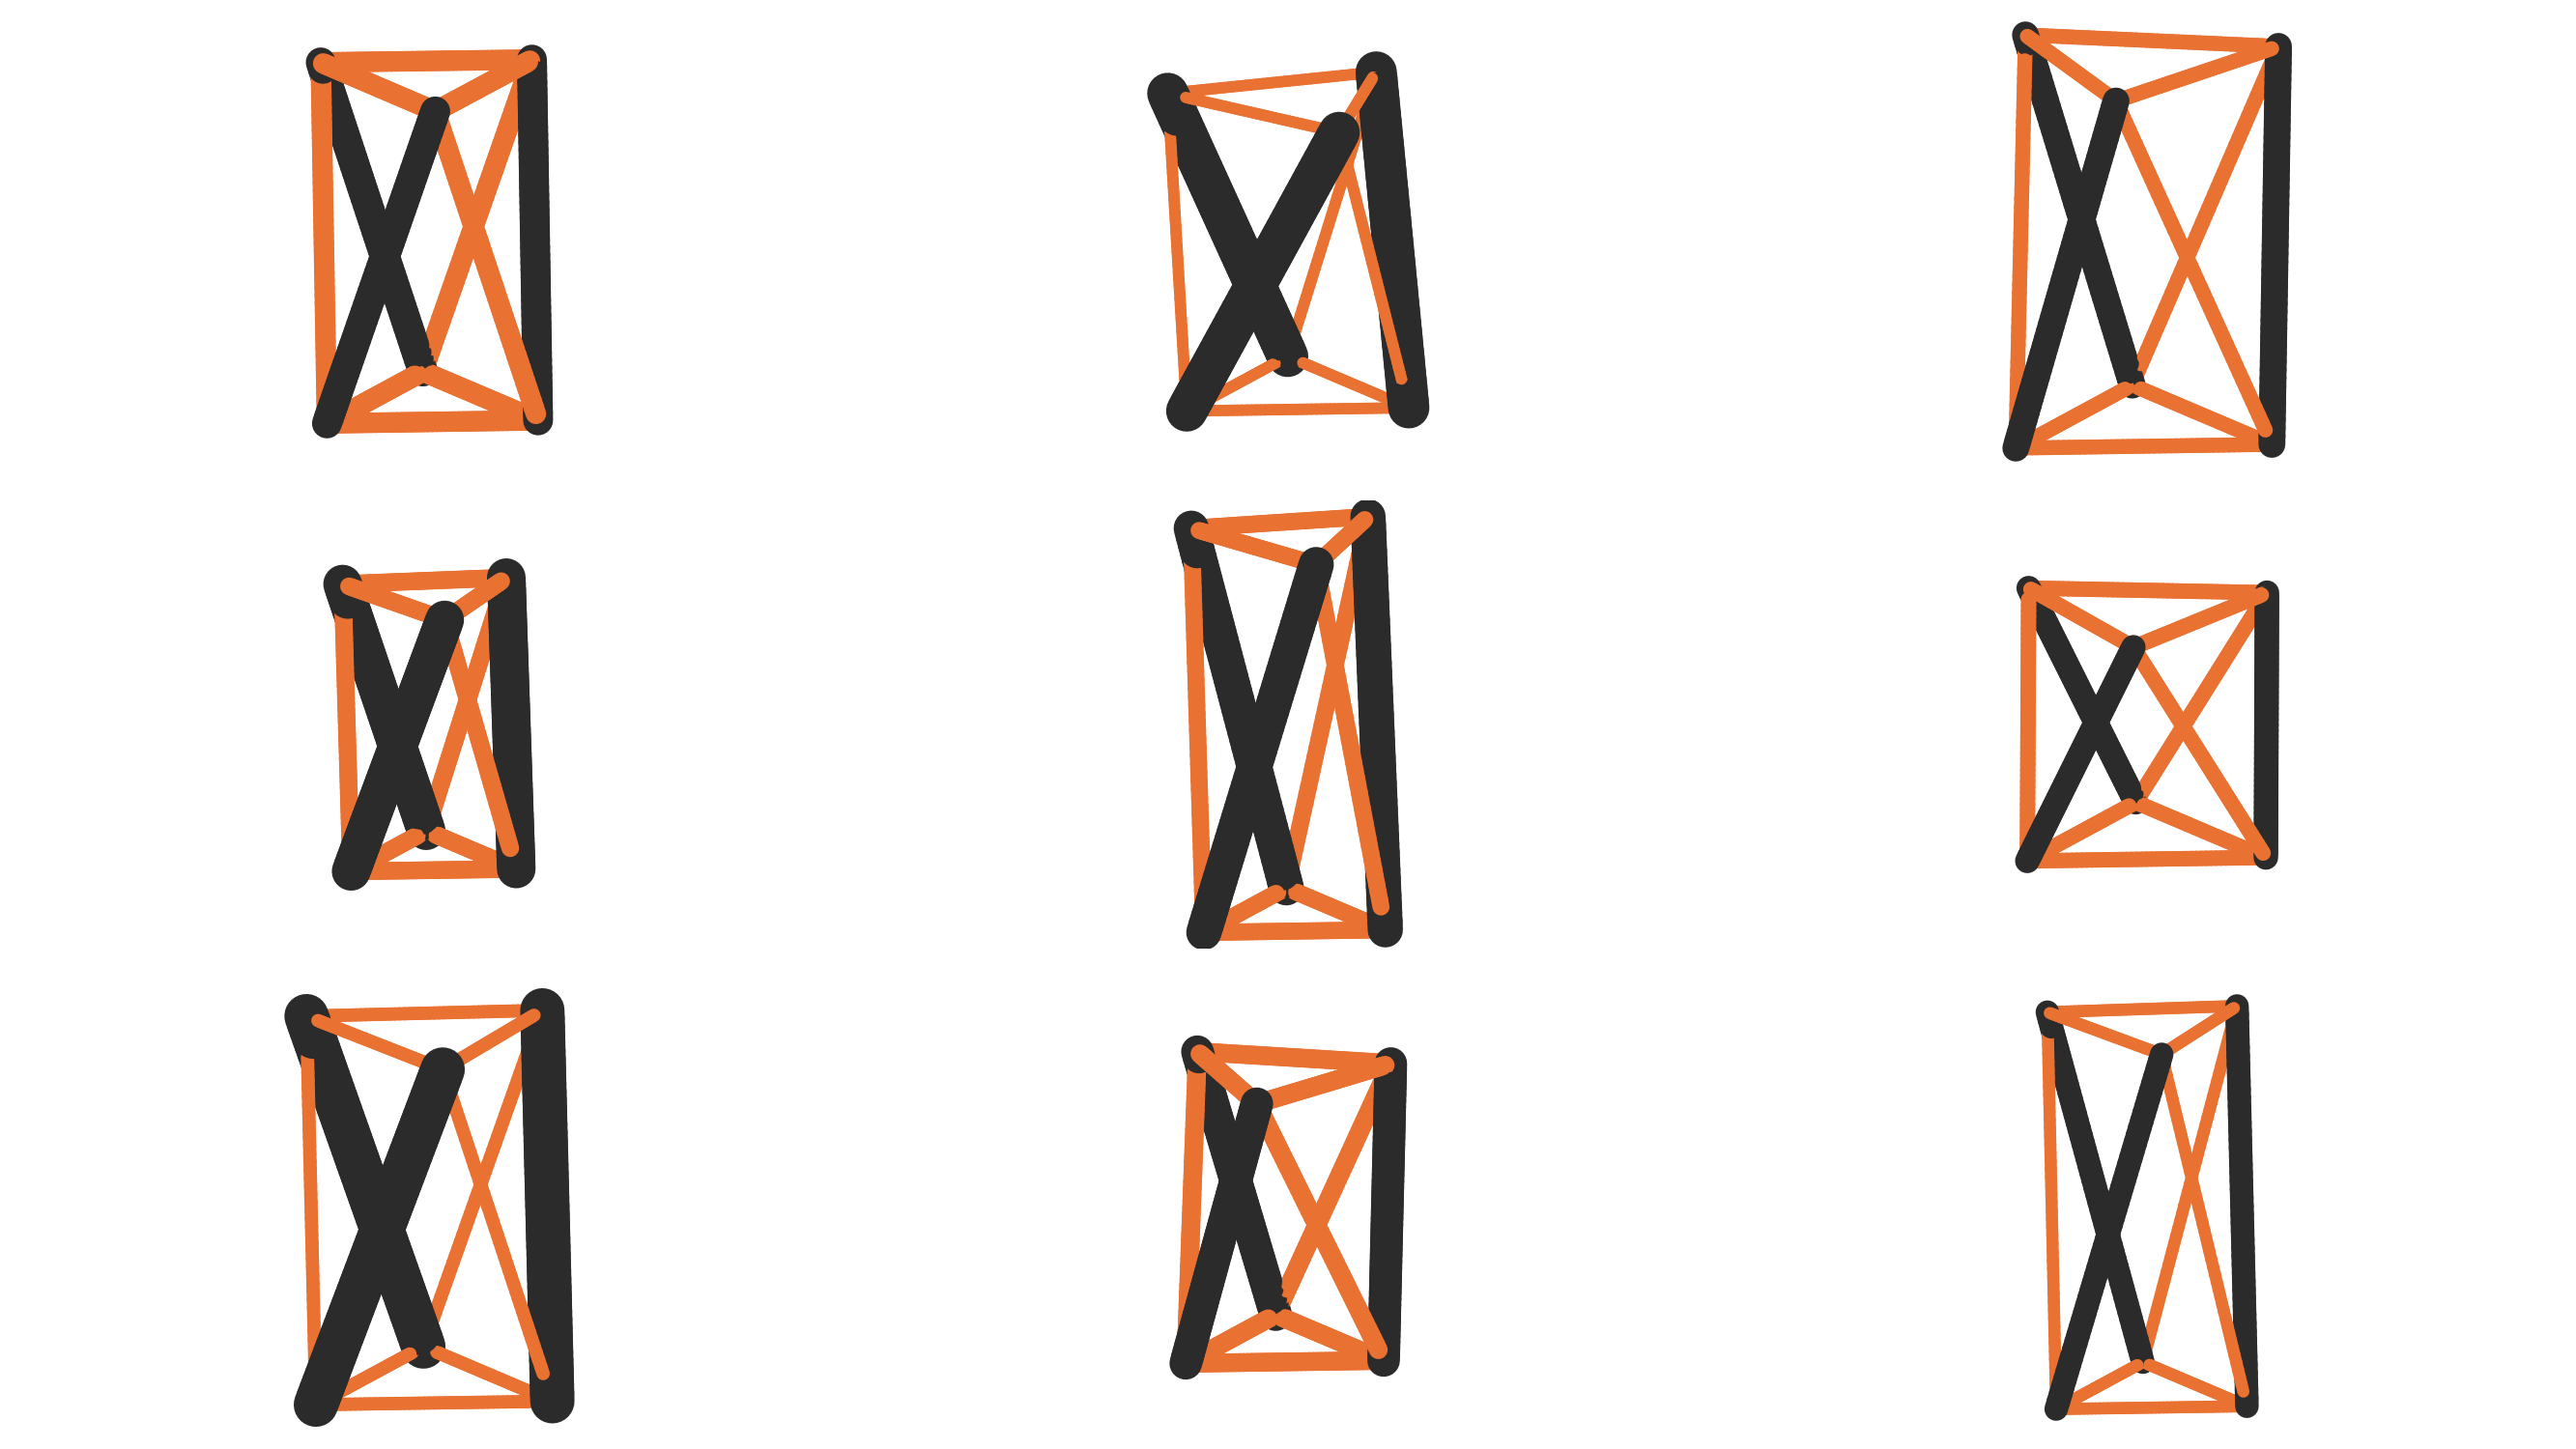
\includegraphics[width=\linewidth]{../figures/bo/fig-seed-designs.png}
  \caption{The nine seed geometries rendered to a common millimeter
    scale (rigid PLA struts in black, TPU tendons in orange). Every
    rendering corresponds to a physically printed article in the seed
    campaign.}
  \label{fig:seed-designs}
\end{figure}

\begin{table*}[t]
  \centering
  \caption{Seed-batch drop-tower results: 101 stabilized captures per
    article (103 for autv5r) at \SI{60}{in} onto the standardized
    polyurethane surface, CFC-180 filtering, counted after the first
    two warm-up drops of each session were discarded. Means $\pm$ one
    standard deviation over the stabilized drops; rows are ordered by
    $t_{180}$. $E_{\mathrm{reb}}$ uses each
    article's weighed mass per Eq.~\eqref{eq:objectives}. The ringdown
    frequency $f_n$ is a print-health descriptor, not an objective.
    A dash denotes a quantity that cannot be computed from the
    available record: article \textit{amdjwm} lacks a weighed mass and
    a confirmed design mapping (it is excluded from the surrogate fit
    and from all mass-dependent quantities), and no accepted $f_n$
    estimate is available for \textit{bag26v} or \textit{ajhby6}.
    Specs 03 and 06 were printed but have no drop sessions in the
    campaign record.}
  \label{tab:seed-results}
  \small
  \begin{tabular}{@{}llS[table-format=2.2]S[table-format=1.4]@{\,$\pm$\,}S[table-format=1.4]S[table-format=2.1]S[table-format=3.0]@{}}
    \toprule
    Design & Article & {Mass (g)} & \multicolumn{2}{c}{$t_{180}$} &
    {$E_{\mathrm{reb}}$ (mJ)} & {$f_n$ (Hz)} \\
    \midrule
    Spec 01 & 6lhxfy & 18.50 & 0.8931 & 0.0042 & 13.9 & 368 \\
    (unmapped) & amdjwm & {-} & 0.9805 & 0.0025 & {-} & 455 \\
    Spec 05 & 6nheas & 21.73 & 0.9970 & 0.0032 & 13.1 & 322 \\
    S0 ref. & bpx68c & 20.23 & 1.0111 & 0.0024 & 6.2 & 468 \\
    Spec 07 & ajhby6 & 20.53 & 1.0127 & 0.0038 & 6.1 & {-} \\
    Spec 00 & 9hhbkp & 21.62 & 1.0183 & 0.0017 & 6.9 & 364 \\
    Spec 04 & nvxsrv & 20.66 & 1.0275 & 0.0044 & 8.2 & 294 \\
    Spec 02 & autv5r & 22.04 & 1.0404 & 0.0035 & 8.8 & 386 \\
    Spec 08 & bag26v & 21.42 & 1.0616 & 0.0051 & 7.7 & {-} \\
    \bottomrule
  \end{tabular}
\end{table*}

\subsection{Model-Recommended Batches and Replication}
\label{sec:results:batches}

Table~\ref{tab:batch-results} reports the stabilized objectives for
the three model-recommended batches, and
Fig.~\ref{fig:front-evolution} overlays every measured article with
the non-dominated front after each batch (Pareto membership is
evaluated over articles with both objectives; the unmapped seed
article amdjwm is omitted because its missing weighed mass prevents
computing $E_{\mathrm{reb}}$). Dominated hypervolume, evaluated at
the fixed reference point $(t_{180}, E_{\mathrm{reb}}) =
(1.35, \SI{15}{mJ})$, grew from 3.155 after the seed batch to 3.969
after batch 2 ($+25.8\%$), 4.007 after batch 3 ($+0.9\%$), and 5.195
after batch 4 ($+29.7\%$): a 65\% total gain over the seed front. No
budget-matched quasi-random physical baseline has been run, so the
comparison the data support is against the campaign's own Sobol
seed: after batch 4, every member of the combined front (corny7,
corny6, drran5, drran3, r2d2c6) is a model-recommended design, and
the last seed article left the front when the batch-4 record
dominated it outright.

\paragraph{Batch 2 (Ax trials 10 to 18)} The first recommended batch
was generated from the seed fit and printed under the
constant-solid-mass projection, so its printed masses still spread
widely (17.91 to \SI{23.47}{g}; a regenerated constant-printed-mass
recommendation set is archived alongside the as-printed one, and the
two must not be conflated). The batch grew the front almost entirely
on the rebound axis: r2d2c6's \SI{4.1}{mJ} per drop is the lowest
rebound on record and still stands, and four batch-2 articles joined
the front. On the transmissibility axis the batch humbled its own
forecasts: the archived posterior predictions sat below the
measurements for nine of nine articles (mean absolute percentage
error 14.4\%; worst case r2d2c3, predicted 0.910, measured 1.334,
the strongest amplifier in the campaign record). That nine-of-nine
optimism widened the refit posterior for every batch that followed.

\paragraph{Batch 3 (Ax trials 28 to 36)} The first batch at constant
\emph{printed} mass (19.24 to \SI{20.06}{g}, CV 1.7\%) and the first
with the infill and filament axes active
(Section~\ref{sec:methods:parameterization}). It filled the knee of
the front rather than growing the box ($+0.9\%$ hypervolume; three
articles joined), and the recalibrated posterior held: eight of nine
articles measured within 0.3 posterior standard deviations of their
predictions (MAPE 3.8\%). The batch also delivered the campaign's
sharpest single surprise in both directions: the best-predicted
design (trial 32, predicted 1.020) measured 1.251, the strongest
amplification then on record, while the batch's only attenuator
(drran8, 0.980, drift-flagged, provisional) was its only twisted
design.

\paragraph{Batch 4 (Ax trials 37 to 45)} The acquisition split the
batch between the wide, high-twist, thin-cable family it had been
steering toward since batch 2 and a previously unvisited tall,
low-twist corner. The wide family delivered: four of nine articles
attenuate, and corny7, the batch's best-predicted design (trial 37,
predicted $0.934 \pm 0.13$), measured $t_{180} = 0.8031 \pm 0.0025$,
the strongest attenuation in the program, 10\% below the best seed
article and 21\% below the reference prism, at a mid-pack
\SI{9.4}{mJ} rebound; it dominates the seed attenuator on both
objectives (Fig.~\ref{fig:batch4-pred-vs-meas}). Within the
attenuating family the frozen predictions ranked the four
measurements perfectly (Spearman $\rho = +1.0$; $0.82$ across all
nine, where the five amplifier predictions span only 0.9\% and so
carry no ordering signal), batch MAPE was 6.0\%, and no article left
its predictive band by more than one standard deviation (the record
itself beat its band by 1.0 standard deviation in the good
direction). Per the between-seat replication rule, the batch-4
attenuation values, including the record, are single-seating
measurements whose re-seat confirmations are scheduled; one session
(corny5) carries a drift flag and its mean is provisional, and
another (corny6) was erratic (per-drop CV 2.0\%) but attenuates
under any reading of its record.

\paragraph{Replication: a second pass of batch 3} The batch-3 plate
was printed a second time (nine design replicates, the reprint
weighing \SI{0.27}{g} heavier article for article on average) and
the second set was drop-tested under the identical protocol, 360
drops across the two passes. Neither extreme of the first pass
recurred. Under \emph{any} pairing of the blinded session labels,
the design that measured 1.251 re-measured at most 1.090 (a drop of
at least 13\%) and the 0.980 attenuator re-measured at least 1.011,
so batch 3 contains no reproducibly attenuating design; under the
best-fit pairing, the same-design shifts have median $+1.2\%$, five
of nine fall inside the previously characterized $\pm 2.2\%$ re-seat
envelope, and the tails reach $-13.8\%$. The two passes cannot
separate seating effects from print-to-print differences, but the
methodological conclusion does not depend on that split: the 1.251
session had passed every within-session stability check (per-drop CV
0.77\%, no drift), so \emph{within-session stability does not
certify a measurement as a design property}. The between-seat
replication rule of Section~\ref{sec:methods:testing} was adopted in
response, the seed attenuator's 0.13\% agreement across an
independent re-seat shows that genuine attenuation does reproduce,
and a broadband seat gauge (the ratio of CFC-1000 to CFC-180
transmissibility; healthy sessions read 1.00 to 1.07) now
accompanies the rule as an advisory: every large same-design shift
observed so far carried a gauge reading of at least 1.15 in one of
its seatings, and all four batch-4 attenuators gauge healthy (0.98
to 1.06).

\begin{table*}[t]
  \centering
  \caption{Model-recommended batch results under the protocol and
    reporting conventions of Table~\ref{tab:seed-results} (CFC-180,
    stabilized means $\pm$ one standard deviation; about twenty
    drops per article against the seed batch's 101, with exact
    per-session counts in the archived per-drop records; rows
    ordered by $t_{180}$ within each batch).
    $E_{\mathrm{reb}}$ uses each article's weighed mass per
    Eq.~\eqref{eq:objectives}. ``Pred.'' is the posterior-mean
    $t_{180}$ archived when the batch was recommended, before any of
    its articles were tested. Batch-2 articles were projected to
    constant solid mass; batches 3 and 4 to constant printed mass
    (\SI{20.23}{g}). Flags follow the session record: $\dagger$
    marks a transmissibility-drift-flagged session whose mean is
    provisional, and $\ddagger$ marks the erratic corny6 session
    (per-drop CV 2.0\%).}
  \label{tab:batch-results}
  \small
  \begin{tabular}{@{}clcS[table-format=2.2]S[table-format=1.4]@{\,$\pm$\,}S[table-format=1.4]S[table-format=2.1]S[table-format=1.3]@{}}
    \toprule
    Batch & Article & Trial & {Mass (g)} & \multicolumn{2}{c}{$t_{180}$} &
    {$E_{\mathrm{reb}}$ (mJ)} & {Pred.\ $t_{180}$} \\
    \midrule
    2 & r2d2c7 & 15 & 18.51 & 0.9484 & 0.0008 & 12.2 & 0.905 \\
    2 & r2d2c1 & 13 & 19.38 & 0.9942 & 0.0021 & 6.0 & 0.948 \\
    2 & r2d2c2$^\dagger$ & 12 & 17.96 & 1.0411 & 0.0154 & 5.6 & 0.926 \\
    2 & r2d2c9 & 10 & 17.91 & 1.0530 & 0.0035 & 5.8 & 0.873 \\
    2 & r2d2c6 & 14 & 19.11 & 1.0548 & 0.0042 & 4.1 & 0.953 \\
    2 & r2d2c8 & 17 & 19.98 & 1.0704 & 0.0116 & 7.9 & 0.955 \\
    2 & r2d2c5 & 18 & 23.47 & 1.1516 & 0.0040 & 6.7 & 0.987 \\
    2 & r2d2c4 & 11 & 19.33 & 1.1847 & 0.0076 & 6.4 & 0.885 \\
    2 & r2d2c3 & 16 & 18.63 & 1.3337 & 0.0117 & 5.6 & 0.910 \\
    \midrule
    3 & drran8$^\dagger$ & 35 & 19.32 & 0.9804 & 0.0051 & 11.2 & 1.039 \\
    3 & drran1 & 36 & 19.31 & 1.0326 & 0.0016 & 18.1 & 1.051 \\
    3 & drran4 & 29 & 19.92 & 1.0344 & 0.0017 & 9.1 & 1.032 \\
    3 & drran2 & 33 & 19.33 & 1.0345 & 0.0006 & 11.8 & 1.056 \\
    3 & drran5 & 28 & 19.88 & 1.0373 & 0.0024 & 5.0 & 1.059 \\
    3 & drran3 & 31 & 19.92 & 1.0389 & 0.0012 & 4.2 & 1.043 \\
    3 & drran9 & 30 & 19.34 & 1.0425 & 0.0009 & 5.2 & 1.058 \\
    3 & drran6 & 34 & 19.24 & 1.0471 & 0.0040 & 4.8 & 1.065 \\
    3 & drran7 & 32 & 20.06 & 1.2513 & 0.0096 & 8.2 & 1.020 \\
    \midrule
    4 & corny7 & 37 & 19.62 & 0.8031 & 0.0025 & 9.4 & 0.934 \\
    4 & corny9 & 43 & 19.46 & 0.8766 & 0.0036 & 18.1 & 0.942 \\
    4 & corny6$^\ddagger$ & 41 & 19.45 & 0.9106 & 0.0181 & 5.7 & 0.943 \\
    4 & corny8 & 39 & 19.64 & 0.9535 & 0.0025 & 17.5 & 0.954 \\
    4 & corny1 & 42 & 20.20 & 1.0459 & 0.0029 & 8.7 & 1.010 \\
    4 & corny4 & 44 & 20.56 & 1.0475 & 0.0025 & 4.3 & 1.013 \\
    4 & corny3 & 45 & 20.15 & 1.0705 & 0.0013 & 8.8 & 1.004 \\
    4 & corny2 & 38 & 20.21 & 1.0846 & 0.0030 & 9.2 & 1.008 \\
    4 & corny5$^\dagger$ & 40 & 20.58 & 1.0876 & 0.0099 & 8.5 & 1.012 \\
    \bottomrule
  \end{tabular}
\end{table*}

\begin{figure*}[t]
  \centering
  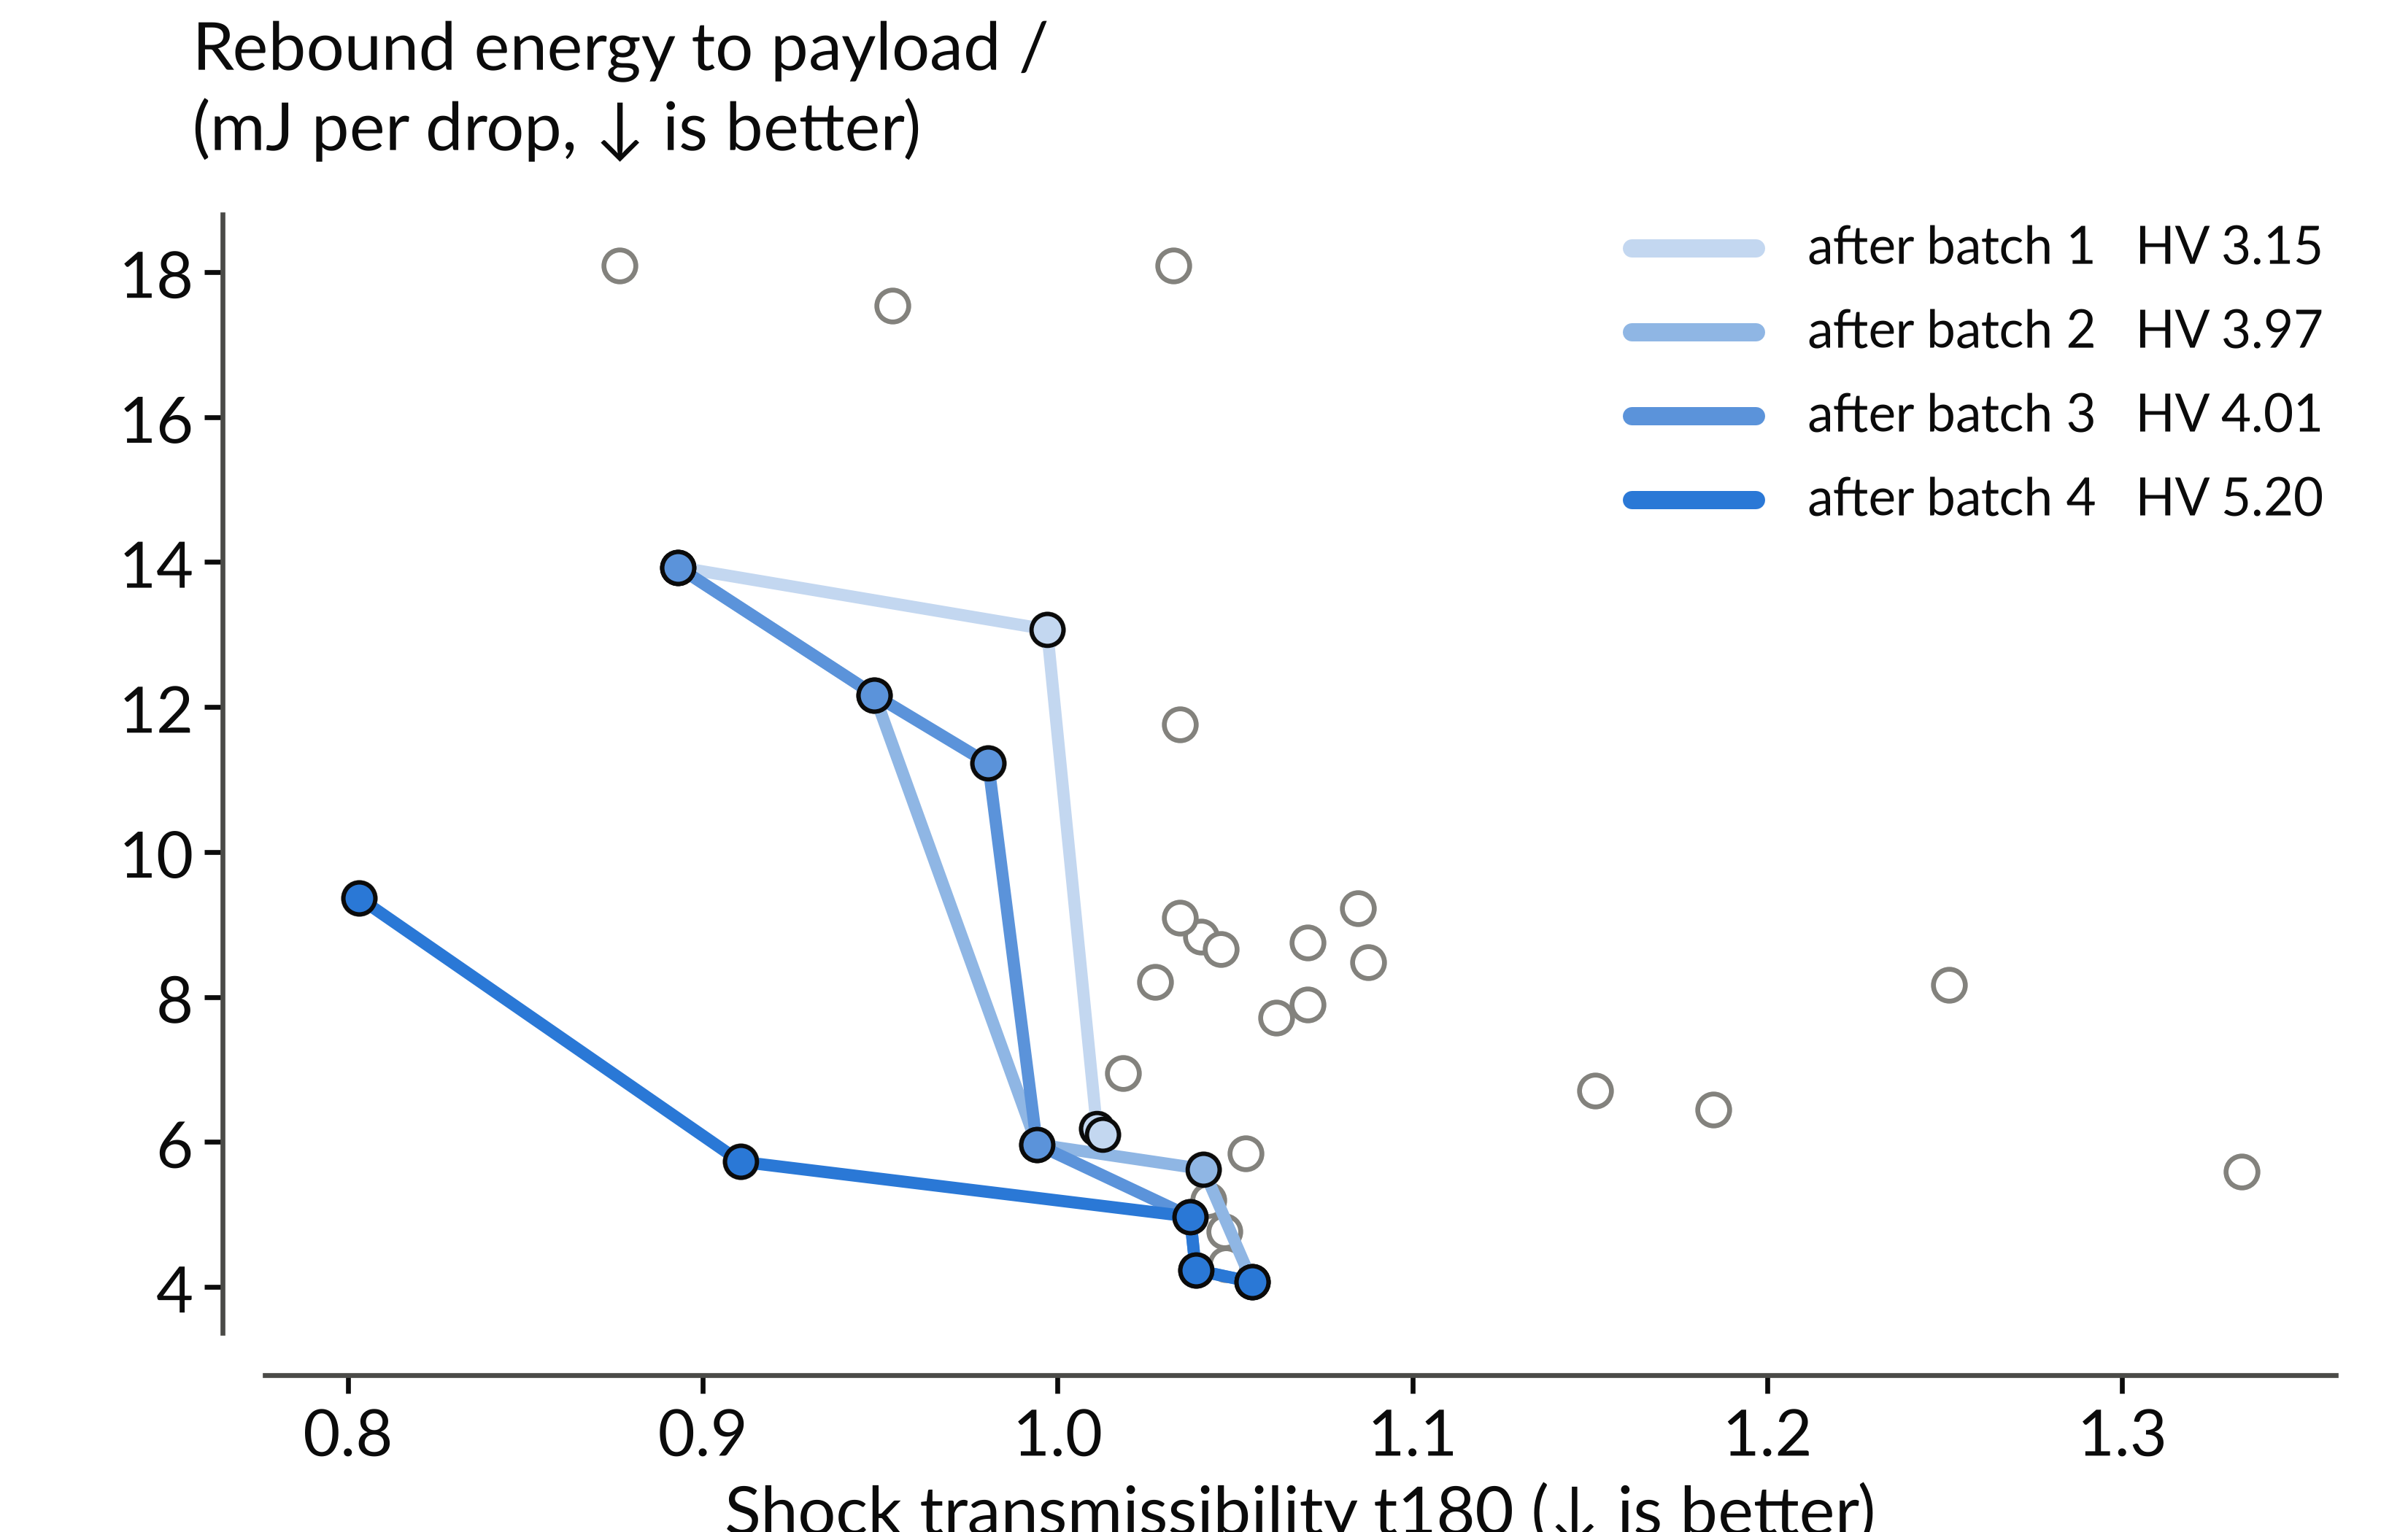
\includegraphics[width=0.85\textwidth]{../figures/bo/t3-prism-bo-front-evolution.png}
  \caption{Measured objective space and front evolution across the
    four batches. Gray circles are all measured articles at their
    stabilized means; the blue lines are the non-dominated fronts
    after each batch, with the dominated hypervolume at the
    $(1.35, \SI{15}{mJ})$ reference in the legend. Batch 2 grew the
    front on the rebound axis, batch 3 filled the knee, and batch 4
    broke the transmissibility floor. Both axes improve downward.}
  \label{fig:front-evolution}
\end{figure*}

\begin{figure*}[t]
  \centering
  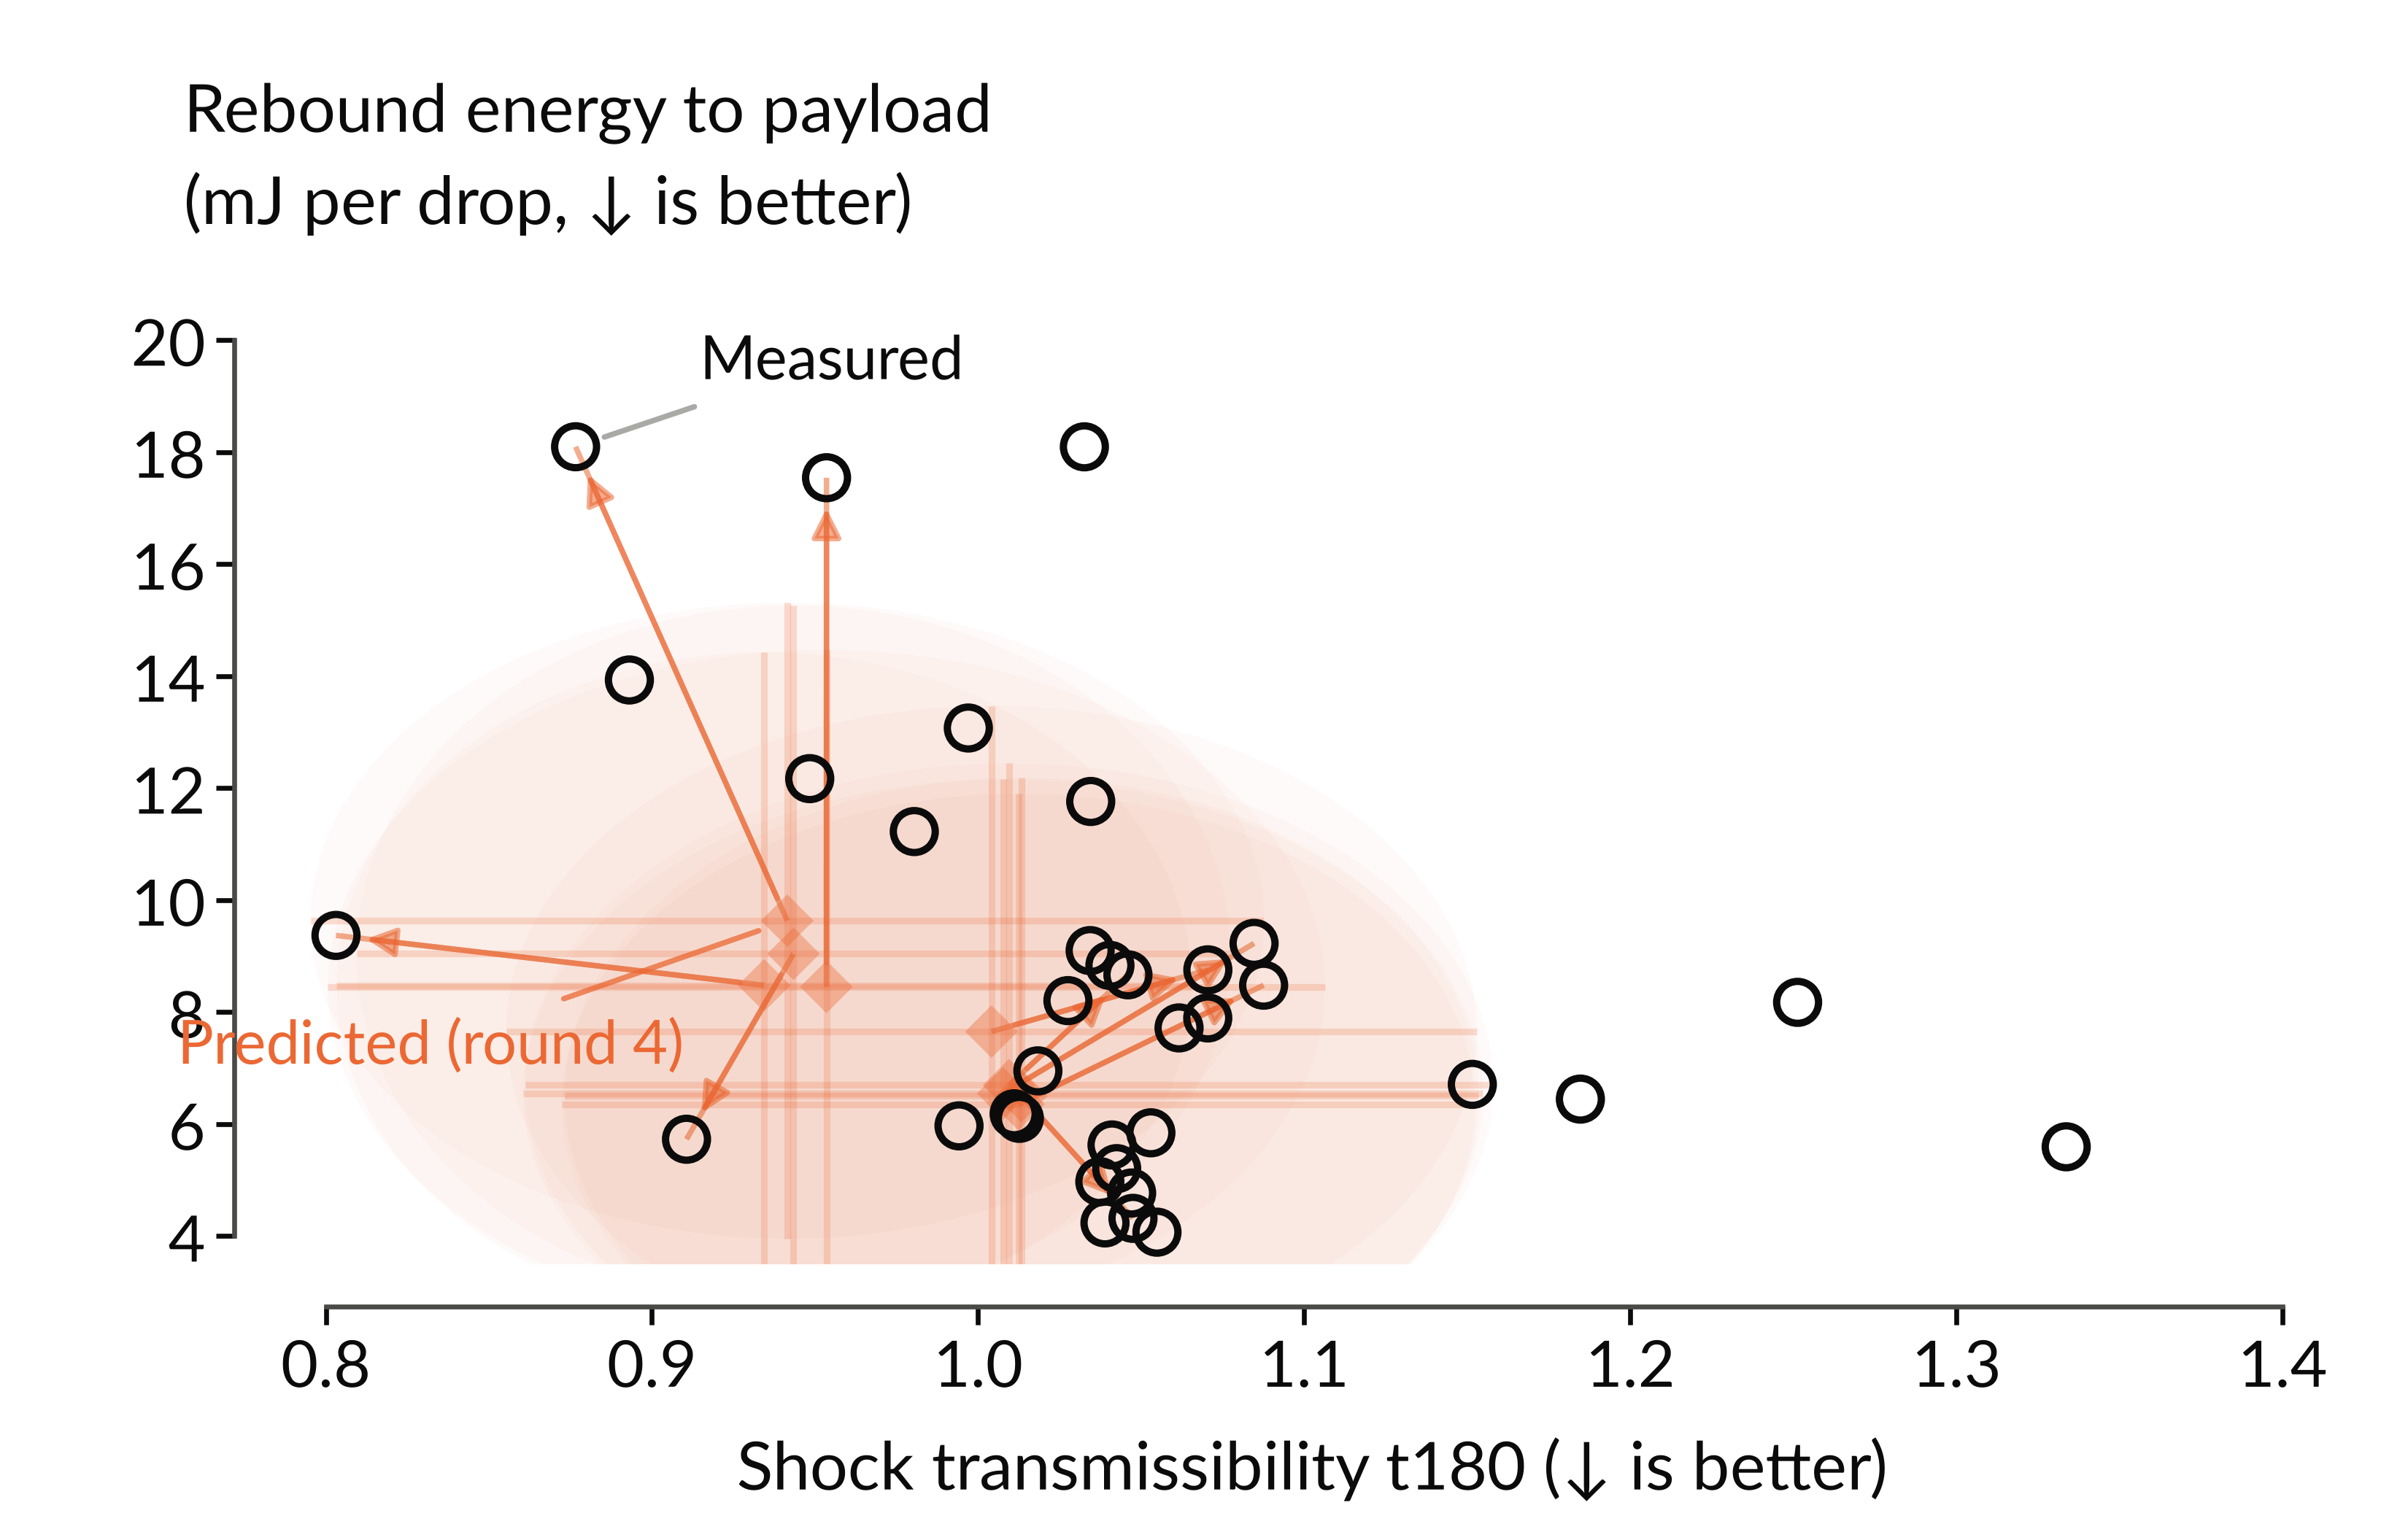
\includegraphics[width=0.85\textwidth]{../figures/bo/t3-prism-bo-round4-predicted-vs-actual.png}
  \caption{Batch-4 predictions against outcomes. Orange diamonds with
    bars are the archived posterior predictions (mean $\pm$ one
    standard deviation) for trials 37 to 45 at recommendation time;
    arrows connect each prediction to its article's measured value
    (black circles; all previously measured articles shown for
    context). The record attenuator corny7 (measured 0.803) is the
    left-most measured point. Both axes improve downward.}
  \label{fig:batch4-pred-vs-meas}
\end{figure*}

\subsection{Surrogate Audits Across the Campaign}
\label{sec:results:audits}

Each refit is audited with leave-one-out cross-validation (LOOCV;
one full NUTS refit per held-out article) and length-scale
diagnostics. Figure~\ref{fig:sensitivity} reports the seed-state
SAASBO feature importances (normalized inverse length scales, median
over the Monte Carlo draws with interquartile whiskers, over the five
design variables plus printed mass). At seven observations for six
correlated inputs these are prior-sensitive model diagnostics only:
no input separates decisively from the equal-share line, and none
supports a claim of variable relevance or ranking.

The honest headline of the cross-validation trajectory is that
held-out point accuracy \emph{declined} as the campaign grew:
$t_{180}$ LOOCV MAPE was 2.9\% with rank correlation $+0.76$ on the
seed state (8 articles, 6 model inputs), 5.4\% and $+0.60$ after
batch 2 (17 articles), and 6.2\% and $+0.19$ after batch 3 (26
articles, 12 inputs); the rebound channel reads 29.3\%, 23.6\%, and
32.2\% MAPE at the same states
(Fig.~\ref{fig:loocv}; the fold-level records are archived with the
campaign data). Three changes landed together and are confounded:
the input space doubled from 6 to 12 while the data grew only from
17 to 26, four of the six added axes carry a single value per batch
and are therefore perfectly confounded with batch, and batch 3
itself added the campaign's largest outliers. The held-out posterior
shrinks predictions toward the pooled mean, so the campaign's
defining extremes are exactly what it misses. The practical stance
this trajectory dictates, and the one the campaign took, is to treat
predicted columns as exploration bookkeeping rather than forecasts:
batch 4's value was the design family it selected and the record it
found, not its point accuracy, and its best-predicted article was
the record. Two further audit facts round out the picture. The
mass-transmissibility correlation fell from $r = 0.82$ over the
seed articles to $0.07$ over the 26 articles of batches 1 to 3, so
the constant-printed-mass projection removed the seed batch's
dominant confound. And the planned head-to-head calibration
comparison against a point-estimated single-task GP with the same
kernel has not yet been run, so no claim is made that SAASBO
outperforms it here.

\begin{figure}[t]
  \centering
  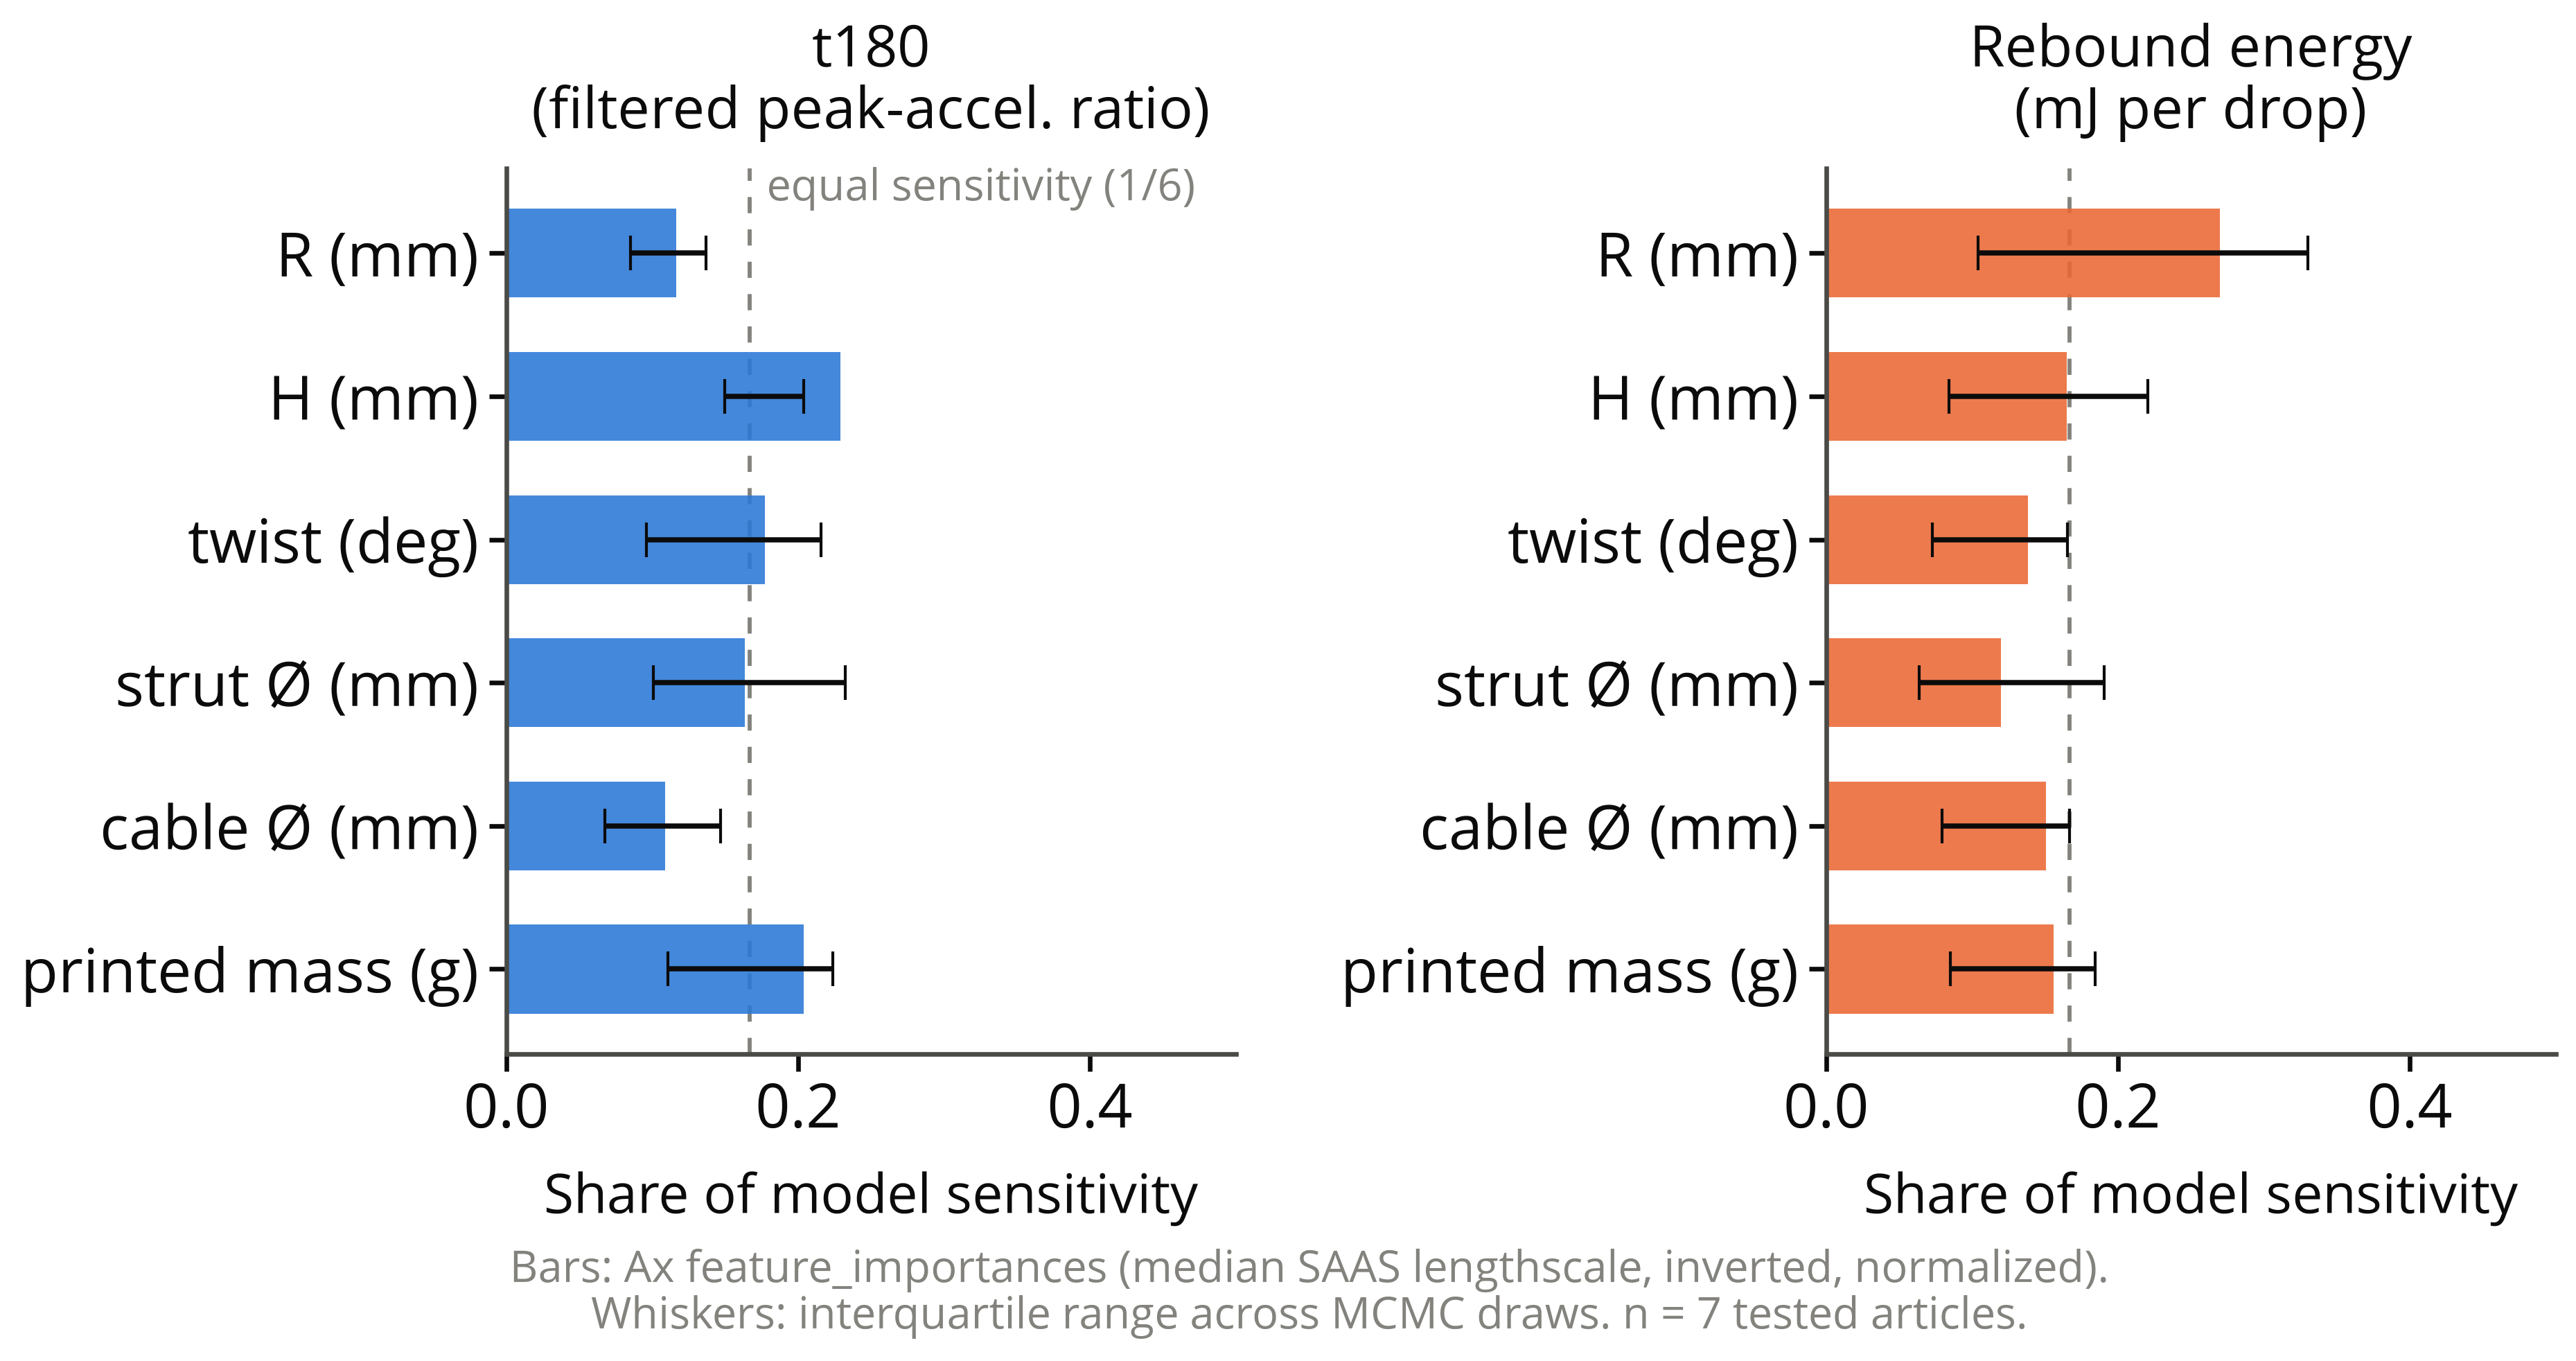
\includegraphics[width=0.92\linewidth]{../figures/bo/t3-prism-bo-round1-feature-importance.png}
  \caption{Seed-state SAASBO length-scale diagnostics per objective
    (normalized inverse length scales; median over MCMC draws,
    interquartile whiskers; inputs are the five design variables plus
    printed mass; the horizontal axis, labeled ``share of model
    sensitivity'' in the plot, is this normalized inverse-length-scale
    diagnostic). No input separates decisively from the equal-share
    line (dashed) at seven mapped articles, and these are
    prior-sensitive model diagnostics, not evidence of variable
    relevance.}
  \label{fig:sensitivity}
\end{figure}

\begin{figure}[t]
  \centering
  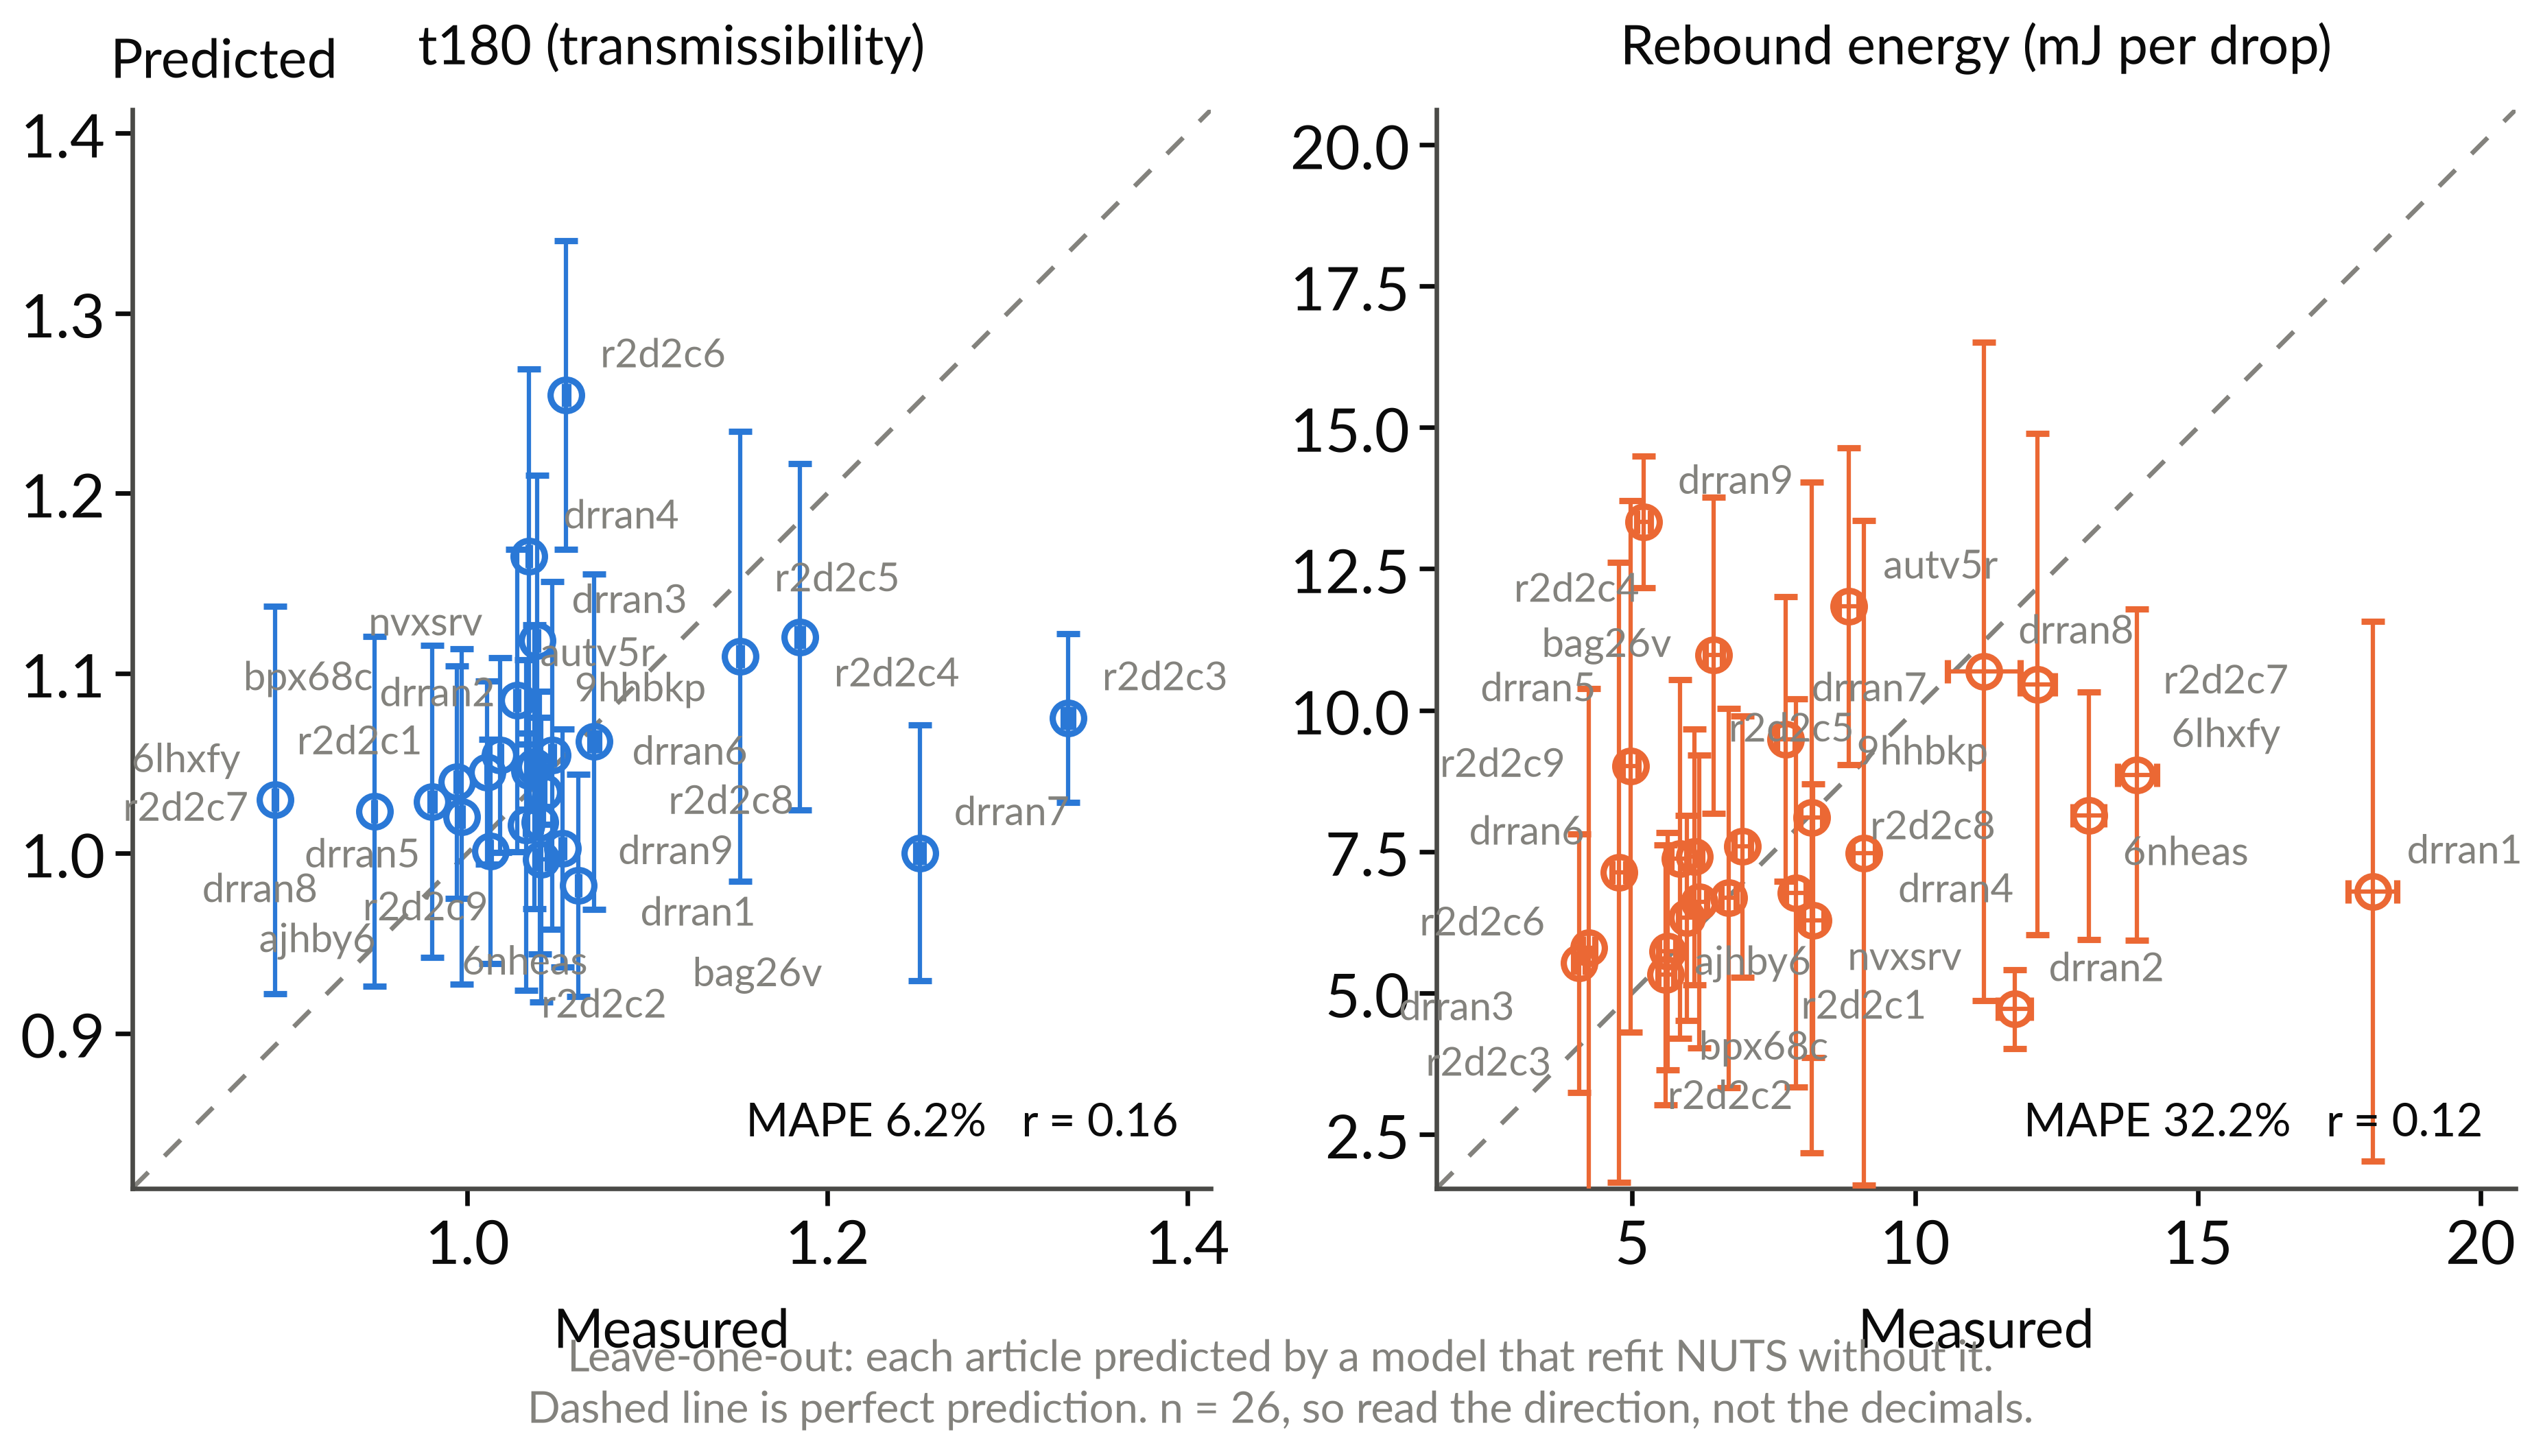
\includegraphics[width=0.92\linewidth]{../figures/bo/t3-prism-bo-round4-loocv.png}
  \caption{Leave-one-out cross-validation of the SAASBO surrogate on
    the 26 articles of batches 1 to 3 (one full NUTS refit per
    held-out article; 12 model inputs). Vertical bars are one
    posterior standard deviation of the held-out prediction;
    horizontal bars are the measured standard error as ingested. The
    dashed line is parity. The held-out posterior shrinks toward the
    pooled mean, so the extremes (r2d2c3, drran7, the seed
    attenuator) are the largest misses.}
  \label{fig:loocv}
\end{figure}

\paragraph{Studies pending} The re-seat confirmations of the batch-4
attenuators (the record article first), any batches beyond the
fourth (a fifth batch is generated and its print files staged, but
nothing from it appears here), the replicate rank-stability study of
Section~\ref{sec:methods:rankstability} (best-, mid-, and
worst-predicted in-sample designs re-printed in nominal triplicate),
the quasi-static crush campaign, and the metal-analog comparison
(Table~\ref{tab:metal-validation}) remain future work; none of their
values appear in this section.


% =============================================================================
\section{Discussion}
\label{sec:discussion}
% =============================================================================

\paragraph{What the campaign establishes} The four measured batches
settle four questions the planned-methods stage could only pose. The
end-to-end loop runs and closes, repeatedly: printed articles,
instrumented characterizations, a fitted fully Bayesian surrogate,
and three successive model-recommended batches whose own
measurements fed the next refit. The measurement distinguishes the
tested articles: the campaign $t_{180}$ means span 0.803 to 1.334,
far beyond within-session drop scatter, though
the batch-3 second pass shows that seating and print variation, not
drop scatter, set the resolution floor for any single article. The
physics is more adversarial than the cushioning intuition suggests:
at this scale and rate, most printed prisms \emph{amplify} the peak
shock reaching their top vertex (26 of 35 articles measured above
unity), which sharpened the campaign question from ``how much does
the architecture cushion'' to ``which corner of the design space
crosses into attenuation, and at what rebound cost.'' And the
batches answered that sharpened question, though not on the first
try: batch 2's forecasts were optimistic on nine of nine articles,
batch 3's best-predicted design was its worst amplifier, and batch 4
then delivered four attenuators from the wide, high-twist,
thin-cable family, led by its best-predicted design at
$t_{180} = 0.803$. The strongest attenuators still tend to carry
large rebound energies (the record article is mid-pack at
\SI{9.4}{mJ}, while the tall batch-4 family shows that near-unity
transmission with low rebound is reachable), so the front remains
genuinely two-dimensional.

\paragraph{Honest accounting of the objective stack} We
pre-registered an adversarial, data-first review of the objective
choices with an external AI referee that was required to commit to
its own objective set from the raw campaign files before reading
ours. Its findings temper the round-1 formulation and set the round-3
revision: the rebound fraction $e_{\mathrm{reb}}$ rests on a ballistic
interpretation of the second contact event that has not yet been
validated against synchronized video (a restrained-versus-unrestrained
check is scheduled); the apparent $t_{180}$-versus-rebound trade-off
is driven substantially by the single strongest attenuator (Spearman
$\rho = -0.39$, $p = 0.38$ across the reliable articles); and
per-drop standard errors are substantially smaller than the
between-article variation, and therefore understate design-level
uncertainty. The campaign's responses were physical rather than
statistical: the batch-3 plate was printed and tested twice, which
measured the same-design shift distribution directly (median
$+1.2\%$, heavy tails; Section~\ref{sec:results:batches}); the
between-seat replication rule now gates every extreme; rebound stays
a candidate constraint pending its ballistic validation; and the
constant-printed-mass projection removed the mass channel the review
flagged. We report this trajectory rather
than presenting the seed-state choices as final because the loop is
the contribution and revising objectives mid-campaign, with the
revision criteria stated in advance, is how such loops behave in
practice.

\paragraph{Mass as a confound and as a design variable} Holding
solid CAD mass constant did not hold printed grams constant: PLA
prints at partial infill while thin TPU cables print near solid, so
the seed articles span \SIrange{18.50}{22.29}{g}, and among the
mapped seed articles mass and $t_{180}$ are correlated
($r = 0.82$). Printed mass is itself induced by the geometry and is
strongly collinear with member dimensions (light articles \emph{are}
the thick-strut, thin-cable corner by construction), so the seed
observations cannot identify separate geometry and mass effects; a
post hoc mass-adjusted regression would be unstable and would
estimate a different, direct-effect quantity. The campaign's answer
was experimental design rather than adjustment: the calibrated
printed-mass model (Supplementary Information) let batches 3 and 4
compare geometries at fixed printed grams (batch mass CVs of 1.7 and
2.3\%), and the mass-transmissibility correlation across the
articles of batches 1 to 3 fell to $r = 0.07$. The confound was
broken by construction, and the mass-aware rebound objective keeps
grams penalized where they physically matter, in the energy returned
to the payload.

\paragraph{Relation to prior art, and why simulation sits outside
the loop} Relative to Pajunen
et~al.~\cite{pajunen2019design}, the present work varies the geometry
under an optimization loop rather than characterizing a single
fabrication condition; relative to Mo
et~al.~\cite{mo2023accelerated}, the loop's ground truth is physical
measurement, and no simulated number enters the objectives, the
acquisition, or candidate priority. That exclusion is a measured
decision, not an omission: an exploratory multi-engine simulation
study conducted alongside the campaign (rigid-body through
finite-element fidelities, archived in the project repository) could
not reproduce the amplification that dominates the measured record
(rigid-strut models cap the transmissibility near unity while most
printed articles exceed it), predicted design-invariant rebound
where the measurement discriminates strongly, and correlated only
weakly with the measured transmissibility. Its constant-mass
fairness constraints and its diagnosis of the seed batch's
mass-rebound confound did shape the campaign design, which is the
screening role we consider simulation to have earned here; anything
more must first demonstrate prospective predictive skill on
articles it has not seen. The measured near-unity
transmission of most seed articles also cautions against reading the
printed-tensegrity literature's attenuation results as generic: the
as-printed cells here are not pretensioned, and activating genuine
pretension in additively manufactured tensegrity (for example through
shrink-on-treatment routes) is an open direction we deliberately
scope out of the present campaign.

\paragraph{Practical considerations and path forward} TPU-PLA
interface durability under repeated impact remains open: no joint
failed during the repeated-drop measurement sessions (more than
1,400 stabilized captures across 35 articles plus the batch-3
second pass), but because
those sessions were not designed as controlled fatigue tests, the
observation does not establish interface durability, and pull-out
and fatigue characterization of the internal-anchor joint is an area
of planned follow-on work. Sensitivity to
print-process covariates (the print key logs defects, humidity, and
the mid-batch nozzle change for exactly this purpose) and transfer to
other material pairs likewise remain open. In the future we plan
the re-seat confirmations of the batch-4 attenuators, the replicate
rank-stability study of Section~\ref{sec:methods:rankstability}, the
metal-analog rank-transfer comparison of
Section~\ref{sec:methods:validation}, quasi-static testing as an
extension of the characterization
(Section~\ref{sec:methods:testing}), pretension activation, tiled
multi-cell absorbers and lattices~\citep{sabounizawadzka2024experimental},
and miniaturization to crutch-tip envelopes: long-term crutch use is
associated with substantial upper-extremity overuse injury and
ground-reaction-force impulses~\citep{requejo2005upperextremitykinetics,
rasouli2020walkingassistanceusing, manocha2021injuriesassociatedwith,
brasilbarrosdasilva2022painmappingand,
dozono2015peripheralneuropathiesin}; existing
spring-loaded~\citep{segura2007mechanicsofambulation,
zhang2011biomechanicalevaluationof} and
polymer-damped~\citep{macgillivray2016theinfluenceof} tip designs
reduce loading rate but not peak transmitted force, and recent
tensegrity crutch concepts~\citep{gu2026tensegritycrutches} and
open-source 3D-printed crutch
work~\citep{mottaghi2025opensource3dprintable} suggest a plausible
translation path, with adjacent footwear and orthotic lattice
studies~\citep{wang2025porouslatticestructure,
zhang2024pressurereducingdesignof,
janarthanan2024additivemanufacturingof} providing transferable design
heuristics.

\paragraph{Limitations} The measured evidence base is 35 articles
across four batches, but with one mechanical-response article per
design in the fit: only batch 3 has a second printed-and-tested set,
and that replication is what exposed the seating and print
sensitivity, so every single-article extreme, including the batch-4
record, is provisional until its re-seat. The drop protocol probes
one height, one impact surface, and axial loading only; the
specimens never leave the elastic regime, so crush-energy metrics
await the quasi-static campaign; per-specimen energy absorption in
joules is not recoverable from the current rig (the falling-mass and
displacement channels required for a force integral are not
instrumented); the four filament axes carry one value per batch and
are unidentified; the held-out prediction skill of the surrogate
declined as the input space grew
(Section~\ref{sec:results:audits}); one tested seed article lacks a
design mapping, one seed design's official article assignment
carries a recorded discrepancy, and two seed designs have no session
record; and all results are from a single printer, material pair,
and cell topology. The replication rule, the planned re-seat
confirmations, the replicate rank-stability study
(Section~\ref{sec:methods:rankstability}), and the metal-analog
protocol (Section~\ref{sec:methods:validation}) are the designed
responses to these limits.

% =============================================================================
\section{Conclusions}
\label{sec:conclusions}
% =============================================================================

We have presented an experiment-driven Bayesian-optimization
framework for designing multi-material 3D-printed tensegrity-inspired
energy absorbers, with TPU used in place of the traditional tension
elements and PLA members carrying compression most of the time, and
we have run it through the recommend, fabricate, measure, and update
cycle three times on physical hardware. The framework parameterizes a
$T_3$-prism family (five geometry variables, joined in batch 3 by
infill and filament process variables) under a constant-mass fairness
projection, fabricates each candidate in a single multi-material FDM
build with TPU tendons anchored inside the PLA strut ends,
characterizes every article with repeated instrumented drops (101
stabilized captures in the seed batch, about twenty thereafter), and
updates a fully Bayesian Gaussian-process
surrogate~\citep{balandat2020botorch, eriksson2021saasbo} that
recommends the next batch. Across the four measured batches (35
articles), the transmissibility spanned 0.803 to 1.334, most
articles amplified the peak shock, and the model-recommended batches
grew the dominated hypervolume 65\% over the Sobol seed front,
ending with a front whose five members are all model-chosen; the
batch-4 best-predicted design set the program record at
$t_{180} = 0.803$, ten percent below the best seed article, and
awaits its re-seat confirmation under the campaign's replication
rule. A second print-and-test pass of one batch showed that seating
and print variation, not drop-to-drop scatter, bound design-level
claims, which is the workflow lesson we consider most transferable.
The workflow is a candidate for other experimentally
evaluated architected structures whose constitutive response is
difficult to calibrate from first principles, but transfer beyond this
printer, material pair, topology, and axial impact condition remains
untested.

% =============================================================================
% Back matter
% =============================================================================
\section*{Acknowledgment} % ASME requests this exact spelling, singular.

This work was supported by the Brigham Young University Mentored
Research Grant program. The authors thank the undergraduate researchers
who carried out the multi-material printing and impact testing, and the
graduate co-mentor who supported day-to-day operations.
\todo{Confirm exact grant numbers and acknowledge any
NASA/Utah-Space-Grant-Consortium support per
acknowledgment-text guidelines.}

\section*{Funding Data}
\begin{itemize}
  \item Brigham Young University Mentored Research Grant.
\end{itemize}
\todo[inline]{Insert the MRG award number, and add the Utah NASA Space
Grant Consortium award if applicable.}

\section*{Conflict of Interest}
The authors declare no conflict of interest.

% Print the list of pending TODOs at the end -- the [disable] option
% on todonotes hides this automatically in the clean wrapper.
\listoftodos[Pending TODOs and figure/table placeholders]

% -----------------------------------------------------------------------------
% References (ASME numeric style; uses asmejour.bst)
% -----------------------------------------------------------------------------
\bibliographystyle{asmejour}
\bibliography{references}

\end{document}
:
%   \def\TODOOPTS{disable}    % manuscript.tex
%   \def\TODOOPTS{}           % manuscript-todos.tex
% =============================================================================

% PDF/A metadata (added in 2022; required by current asmejour for accessibility)
\DocumentMetadata{%
  lang        = en-US,
  pdfstandard = A-3u,
  pdfversion  = 1.7,
}

% Class options (see asmejour-template.pdf for the full list):
%   * lineno       -- numbered lines for review markup (run pdflatex twice)
%   * singlecolumn -- one-column draft layout (drop for ASME two-column final)
%   * nocopyright  -- suppress ASME copyright footer until acceptance
%   * upint, varvw -- typographic preferences carried over from the template
%   * hyphenate    -- allow hyphenation in typewriter font
\documentclass[lineno,nocopyright,upint,varvw,hyphenate]{asmejour}

\allowdisplaybreaks % from amsmath; multiline equations may break across pages

% --- Additional packages ---
% asmejour already loads: graphicx, hyperref, natbib, amsmath, amssymb,
% xcolor, booktabs, subcaption, caption, lineno, etc. Avoid re-loading those.
\usepackage{siunitx}
% House style: no en dashes anywhere, including ranges; siunitx ranges
% therefore render as "X to Y" rather than "X--Y".
\sisetup{range-phrase = { to }, range-units = single}
% tikz for measurement callouts overlaid on the printed-prototype photograph
% (Fig.~\ref{fig:printed-prototypes}); asmejour already loads graphicx/xcolor.
\usepackage{tikz}
\usetikzlibrary{arrows.meta}
% todonotes for in-margin TODO/figure-placeholder markers; toggled by the
% wrapper file (\TODOOPTS = "disable" hides everything; "" shows all).
\usepackage[\TODOOPTS,colorinlistoftodos,textsize=footnotesize]{todonotes}
\setlength{\marginparwidth}{2cm}

% Convenience macros that vanish along with todonotes when [disable] is set.
\newcommand{\figplaceholder}[3][]{%
  % #1 = optional [width]; #2 = label; #3 = caption / what to draw
  \begin{figure}[ht]
    \centering
    \fbox{\parbox[c][3.2cm][c]{0.85\linewidth}{\centering\textit{Figure
        placeholder: #3}}}%
    \caption{\textit{Placeholder.} #3}
    \label{fig:#2}
  \end{figure}%
  \todo[inline,color=orange!30]{Figure \texttt{#2}: #3}%
}

% Synthetic-placeholder (dummy) data convention. Any value that is a
% stand-in rather than a measurement is typeset in this violet color in
% BOTH wrappers (clean and todos) so no reader can mistake it for data.
% As of 2026-09-15 the Results carry no violet values: the former dummy
% round-2 numbers were replaced by the measured batch 2-4 record
% (manuscript/data/, snapshotted from the campaign branch at e25ebf5).
% The macro stays defined for future placeholders.
\definecolor{dummydata}{RGB}{142,68,173}
\newcommand{\dummy}[1]{\textcolor{dummydata}{#1}}

\newcommand{\tabplaceholder}[2]{%
  % #1 = label; #2 = caption / contents description
  \begin{table}[ht]
    \centering
    \caption{\textit{Placeholder.} #2}
    \label{tab:#1}
    \begin{tabular}{@{}lll@{}}
      \toprule
      Column A & Column B & Column C \\
      \midrule
      \multicolumn{3}{c}{\textit{(table contents pending)}} \\
      \bottomrule
    \end{tabular}
  \end{table}%
  \todo[inline,color=orange!30]{Table \texttt{#1}: #2}%
}

% --- PDF metadata ---
\hypersetup{%
  pdfauthor   = {Jeffrey R. Hill and Sterling G. Baird},
  pdftitle    = {Experiment-Driven Bayesian Optimization of the Impact Response
                 of Multi-Material 3D-Printed Tensegrity-Inspired Structures},
  pdfkeywords = {tensegrity, multi-material 3D printing, Bayesian optimization,
                 impact mitigation, design of experiments},
  pdfsubject  = {Manuscript draft for ASME Journal of Mechanical Design},
}

% --- Journal name (printed in the running head; omit "Journal of") ---
\JourName{Mechanical Design}

\begin{document}

% =============================================================================
% Author block(s) -- one \SetAuthorBlock per author (or per shared affiliation)
% Mark corresponding author(s) with \CorrespondingAuthor (no space before).
% =============================================================================
% Author order per @me-madsen review (PR #20): equal-contribution and
% corresponding-author scheme is \textsuperscript{*} = equal contribution,
% \textsuperscript{\dag} = also equal contribution, \textsuperscript{\ddag} =
% corresponding author (see legend \todo after \maketitle).
\SetAuthorBlock{Marcus E. Madsen\textsuperscript{*}}{%
  Department of Mechanical Engineering,\\
  Brigham Young University,\\
  Provo, UT 84602, USA
}

\SetAuthorBlock{Audrey K. Christiansen\textsuperscript{*}}{%
  Department of Mechanical Engineering,\\
  Brigham Young University,\\
  Provo, UT 84602, USA
}

\SetAuthorBlock{Jinkwan Han\textsuperscript{*}}{%
  Department of Mechanical Engineering,\\
  Brigham Young University,\\
  Provo, UT 84602, USA
}

\SetAuthorBlock{Jeffrey R. Hill\textsuperscript{\dag\ddag}\CorrespondingAuthor}{%
  Department of Mechanical Engineering,\\
  Brigham Young University,\\
  Provo, UT 84602, USA\\
  email: jeff.hill@byu.edu
}

\SetAuthorBlock{Sterling G. Baird\textsuperscript{\dag\ddag}\CorrespondingAuthor}{%
  Department of Mechanical Engineering,\\
  Brigham Young University,\\
  Provo, UT 84602, USA\\
  email: sterling.baird@byu.edu
}

\title{Experiment-Driven Bayesian Optimization of the Impact Response of
       Multi-Material 3D-Printed Tensegrity-Inspired Structures}

% Keywords are printed at the end of the abstract; must precede \end{abstract}.
\keywords{tensegrity, multi-material 3D printing, Bayesian optimization,
          impact mitigation, design of experiments}

% -----------------------------------------------------------------------------
% Abstract -- JMD requires 150--200 words, Latin characters only (no math),
% structured as background, approach, results, conclusions.
% -----------------------------------------------------------------------------
\begin{abstract}
Tensegrity-inspired rigid-soft architectures are candidates for impact
mitigation, but their transmitted-shock response is difficult to predict
from simulation alone. We report an experiment-driven Bayesian
optimization campaign over a co-printed polylactic-acid/thermoplastic-%
polyurethane three-strut prism family. The search space begins with five
continuous geometry variables and, from the third batch, adds
per-article infill densities and batch-level filament settings.
Candidate geometries are projected to a common mass budget and
fabricated in single multi-material builds, and each article is
characterized by repeated instrumented drops: 101 stabilized captures in
the seed batch and about twenty thereafter. The optimizer jointly
minimizes the filtered peak-acceleration ratio (transmissibility) and
the rebound energy returned to the payload. Most printed articles
amplify the peak shock, so the campaign question became which corner of
the design space attenuates. Across one Sobol seed batch and three
model-recommended batches, 35 articles in all, the dominated hypervolume
grew 65 percent, the final Pareto front is entirely model-chosen, and
the fourth batch's best-predicted design set the program record,
lowering transmissibility to 0.803, ten percent below the best seed
article. A second print-and-test pass of one batch showed that seating
and print variation, not drop-to-drop scatter, limit design-level
claims, motivating the replication rule we adopt.
\end{abstract}

\maketitle

\begin{center}
  \fcolorbox{dummydata}{dummydata!6}{\parbox{0.94\linewidth}{\small
  \textcolor{dummydata}{\textbf{Draft note (remove before submission):} this
  draft is written at the intended final scope of the study, and any value
  printed in this violet color is a synthetic placeholder rather than a
  measurement. As of 2026-09-15 the Results contain no violet values: all
  four reported batches (35 articles) are measured data from the committed
  campaign record. Still pending, and written as future work rather than
  as results: the re-seat confirmation of the batch-4 record article, any
  batches beyond the fourth, the replicate rank-stability study (best-,
  mid-, and worst-predicted in-sample designs in nominal triplicate), the
  quasi-static crush campaign, the metal-analog comparison, and the
  archival (Zenodo) code release.}}}
\end{center}

\todo[inline]{\textbf{Author order / contributions (per @me-madsen).} Planned
  order: Marcus E. Madsen\textsuperscript{*}, Audrey K.
  Christiansen\textsuperscript{*}, Jinkwan Han\textsuperscript{*}, Jeffrey R.
  Hill\textsuperscript{\dag\ddag}, Sterling G. Baird\textsuperscript{\dag\ddag},
  where \textsuperscript{*}~=~equal contribution, \textsuperscript{\dag}~=~also
  equal contribution, and \textsuperscript{\ddag}~=~corresponding author.
  Confirm affiliations and add emails for M.~Madsen, A.~Christiansen, and
  J.~Han, and typeset the equal-contribution footnote per ASME JMD style.}

% =============================================================================
% Body -- IMRaD structure per JMD submission instructions
% =============================================================================
\section{Introduction}
\label{sec:introduction}

Tensegrity structures are assemblies of rigid compression members
suspended within a continuous network of tension members; their defining
property, that no two rigid bars touch, yields lightweight assemblies with
remarkable strength-to-weight ratios and tunable nonlinear mechanical
responses~\citep{skelton2009tensegrity, sultan2009tensegrity}. These
properties have made tensegrity attractive across scales, from
metamaterial unit cells~\citep{amendola2014experimental,
zhang2018tensegrity, fraternali2015tensegrity} to compliant impact-absorbing
robots developed for planetary landing~\citep{agogino2018superball,
caluwaerts2014superball, sabelhaus2015system, vespignani2018design,
deitrich2022titan}. Recent work has shown that \emph{tensegrity-inspired}
unit cells can be directly 3D-printed and exhibit load-limiting plateaus
under drop-weight impact~\citep{pajunen2019design}, opening a path
toward additively manufactured architected absorbers. Throughout, we use
\emph{tensegrity-inspired} for printable cells that borrow the separated
compression-member and tension-network geometry of tensegrity while
relaxing defining mechanical conditions of classical tensegrity. In the
present specimens, the TPU tension elements are extensible, the PLA struts
may share printed junctions, and no pretension is activated or measured.
We therefore do not claim classical tensegrity, prestress-stabilized
behavior, or equivalence to an ideal cable-strut prism.

Multi-material fused-deposition modeling (FDM) that pairs a rigid polymer
such as polylactic acid (PLA) with a soft, rate-dependent elastomer such as
thermoplastic polyurethane (TPU) has been used to fabricate rigid-soft
architected energy absorbers on a single platform: thick-panel
origami metamaterials with PLA panels and TPU hinges~\citep{ye2023multimaterial}
and ABS/TPU honeycombs with tunable stiff/flexible
proportions~\citep{khatri2024energy}. The same rigid-soft co-printing
capability makes it possible to rapidly fabricate diverse tensegrity-inspired
geometries, which adopt a discrete-compression/continuous-tension topology
rather than an origami or honeycomb one. Although extruded TPU does not behave
as an idealized
inextensible cable, its rate-dependent damping is a desirable property
for impact-absorption applications and complements the elastic stiffness
of the PLA compression members rather than competing with it.

Designing such architected absorbers is fundamentally a
\emph{design-of-experiments} problem: the configuration space spanned by
strut geometry, tension-element cross-section, connectivity, and
unit-cell tiling is large; each candidate must be physically printed
and tested; and the relevant impact-performance metrics (the shock
transmitted across the structure and the energy returned to the
protected payload) are noisy and partially correlated. Bayesian
optimization (BO) is well-matched to this regime, having driven
breakthroughs from hyperparameter tuning of
AlphaGo~\citep{chen2018bayesianoptimizationalphago} to sustainable
concrete~\citep{ament2023sustainable}, autonomous discovery of organic
laser emitters~\citep{striethkalthoff2024delocalized}, and architected
materials~\citep{mo2023accelerated, zhang2021bo}.
The gap this paper addresses is the combination of these two ideas:
Pajunen et~al.~\cite{pajunen2019design} printed tensegrity-inspired
cells under a single fabrication condition with no optimization loop,
and Mo et~al.~\cite{mo2023accelerated} closed a multifidelity BO loop
entirely in simulation. Among the studies reviewed here, prior work
separately demonstrates physical impact testing of printed
tensegrity-inspired structures, rigid-flexible additive fabrication,
and Bayesian optimization of architected materials; we found no prior
report combining these elements in a BO campaign over co-printed
multi-material tensegrity-inspired hardware with physical impact
measurements as the optimization ground truth. The campaign reported
here closes the recommend, fabricate, measure, and update cycle three
times over: a Sobol seed batch trains the surrogate, and each of three
successive model-recommended batches was fabricated, tested under the
identical protocol, and folded back into the refit that produced the
next.

We emphasize one framing point at the outset: the printed PLA/TPU
$T_3$ prism studied here is a testbed for developing and validating
the closed-loop workflow, not flight hardware, and not the end of the
design space we intend to search. The planetary-lander setting
motivates the objectives (limit the shock delivered to a payload,
limit the energy returned to it) and the constant-mass fairness
constraint, but the contribution is the loop itself: a stepping stone
toward optimizing tensegrity-inspired structures generally, agnostic
to the eventual application scale.

\paragraph{Contributions} This paper makes the following contributions:
\begin{enumerate}
  \item A parameterized family of multi-material 3D-printable
    tensegrity-inspired unit cells that uses TPU in place of the
    tension elements of the traditional tensegrity topology, with PLA
    members that carry compression most of the time (the cells are
    not prestressed, so neither member type acts as a pure tension or
    compression element; under impact some tendons stretch while
    others buckle). The TPU tendons are anchored \emph{inside} the
    ends of each PLA strut, the strut acting as a rigid cage in which
    the cables meeting at a given end join before exiting through
    discrete outlets. This study reports the resulting printable
    joint geometry; pull-out strength and fatigue life remain
    untested and are an area of planned follow-on work. Candidate
    designs are compared fairly through a constant-mass projection
    that rescales every geometry to a common material budget before
    printing (Section~\ref{sec:methods:parameterization}).
  \item A characterized drop-tower protocol and objective stack for
    printed impact absorbers: repeated instrumented drops per article
    (101 stabilized captures in the seed batch, about twenty recorded
    drops in later batches, a reduction justified by the measured
    within-session variance in Section~\ref{sec:methods:testing}),
    standardized SAE~J211 filtering~\citep{saej211}, and two
    per-article objectives, the CFC-180 transmissibility and a
    mass-weighted rebound energy score, each characterized for
    repeatability before entering the optimizer.
  \item An experiment-driven BO loop, built on
    BoTorch/Ax~\citep{balandat2020botorch, pmlr-v293-olson25a} with a
    fully Bayesian sparse-prior surrogate
    (SAASBO)~\citep{eriksson2021saasbo}, that ingests the physical
    drop measurements, models per-print mass explicitly, and
    recommended each next batch of designs to fabricate. All four
    measured batches (35 articles) are reported here; the final
    Pareto front is entirely model-chosen, and the fourth batch's
    best-predicted design set the program attenuation record
    (Sections~\ref{sec:methods:bo} and~\ref{sec:results}).
  \item A measured error budget for drop-tower ranking of printed
    articles: a second print-and-test pass of one full nine-design
    batch (360 additional drops) showing that article seating and
    print-to-print variation, not within-session scatter, set the
    floor for design-level claims, and the between-seat replication
    rule adopted in response (Section~\ref{sec:results:batches}).
\end{enumerate}

The completed evidence in this paper is restricted to single-cell,
fixed-topology $T_3$-prism-inspired specimens under one \emph{axial}
drop condition; quasi-static testing is planned as an extension for
future work. Off-axis and combined loading, controlled fatigue and
damage-accumulation testing, multi-cell behavior, and landing-attitude
variability are likewise future work (Section~\ref{sec:discussion}),
and the novelty and generality claims above are scoped to this
restricted prototype design space rather than to tensegrity-inspired
absorbers in general.

\begin{figure*}[t]
  \centering
  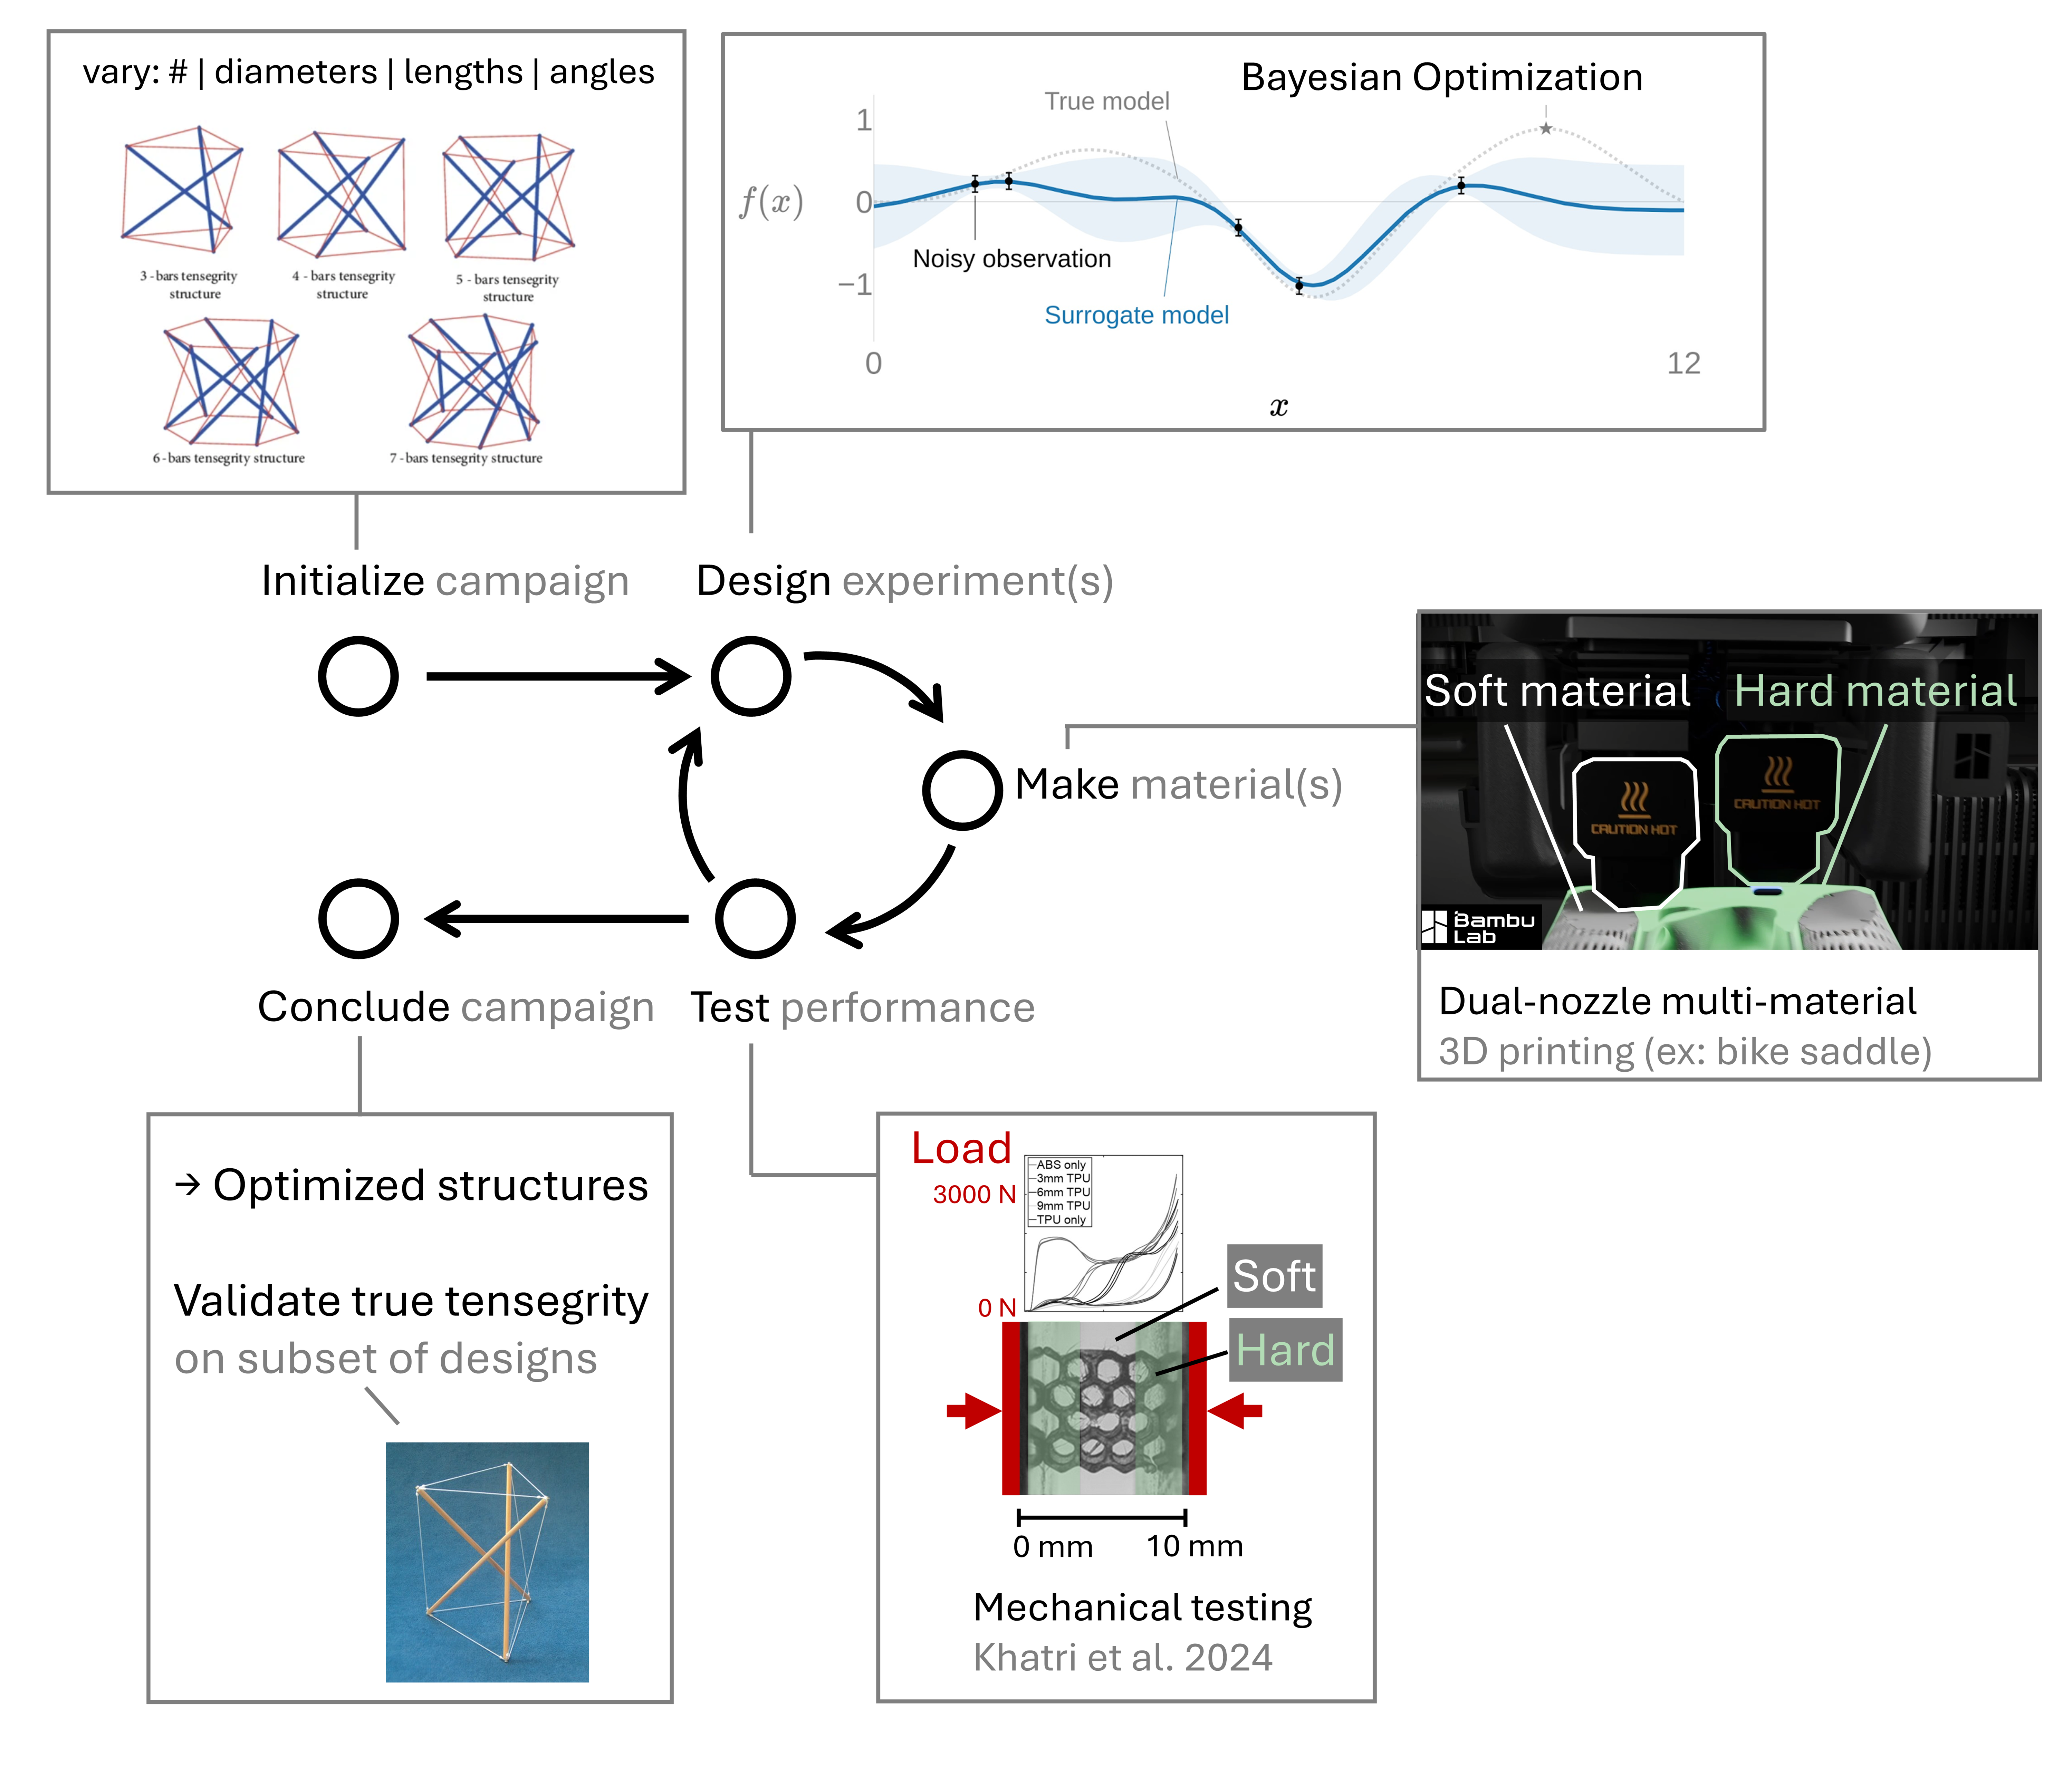
\includegraphics[width=0.7\textwidth]{../figures/overview-updated.png}
  \caption{Closed-loop, experiment-driven design framework. Parameterized
    PLA/TPU tensegrity-inspired unit cells are printed, characterized by
    repeated instrumented drop-weight impacts, and the resulting
    performance data drive a Gaussian-process surrogate that recommends the
    next batch of designs to fabricate.}
  \label{fig:overview}
\end{figure*}%
\todo{Eventually switch this overview figure to a vertical orientation; it is
  currently reproduced from the MRG proposal
  (\texttt{figures/overview-updated.png}).}

The remainder of the paper is organized as follows.
Section~\ref{sec:background} reviews tensegrity mechanics, multi-material
3D printing for energy absorption, and Bayesian optimization with an
emphasis on multi-objective and noise-robust acquisition functions.
Section~\ref{sec:methods} introduces the design parameterization,
fabrication workflow, drop-tower protocol and objectives, and BO loop,
and states the planned metal-analog comparison.
Section~\ref{sec:results} reports all four measured batches, the
surrogate audits, and the replication findings, and
Section~\ref{sec:discussion} discusses the
implications and limitations of the approach. Section~\ref{sec:conclusions}
concludes.

% =============================================================================
\section{Background}
\label{sec:background}
% =============================================================================

\subsection{Tensegrity-Inspired Architectures for Energy Absorption}

Tensegrity prisms and their planar extensions exhibit
softening-stiffening response under
compression~\citep{amendola2014experimental, zhang2018tensegrity,
fraternali2015tensegrity}, characteristics desirable for impact
mitigation because the structure can absorb a large fraction of the
input energy at a controlled, sub-injurious force plateau.
Santos~\cite{santos2023towardanovel} recently characterized a tensegrity
energy-dissipation metamaterial reporting equivalent viscous damping
on the order of $\sim$23\% with negligible residual strain per impact,
underscoring the suitability of tensegrity-inspired architectures for
repeated-impact use cases.
The space program literature documents large-scale tensegrity-inspired
absorbers for planetary landing~\citep{agogino2018superball,
caluwaerts2014superball, sabelhaus2015system, vespignani2018design,
deitrich2022titan} and a long history of crushable energy-absorbing
landing systems~\citep{cloutier1966landing, adams2004merairbag,
jackson2014honeycomb}. Pajunen et~al.~\cite{pajunen2019design} demonstrated that
truncated-tetrahedral tensegrity-inspired unit cells can be directly
3D-printed and exhibit load-limiting plateaus, motivating the present
focus on additively manufactured TPU/PLA composites.
More recent work on dynamically loaded additively-manufactured
energy-absorbing lattices~\cite{davami2019dynamicenergyabsorption}, together
with Intrigila et~al.'s bistable tensegrity-like unit cell for lattice
metamaterials~\cite{intrigila2022fabricationandexperimental} as the closest
published analog, confirms that this architecture class also responds favorably
under impact and quasi-static loading, although neither study employed
multi-material FDM or closed-loop design optimization.
Table~\ref{tab:novelty} situates the present work against selected
prior efforts spanning the three elements combined here (impact-tested
printed tensegrity-inspired structures, rigid-flexible fabrication,
and BO of architected materials), making explicit that, among the
studies reviewed, no single prior study combines a multi-material FDM
tensegrity-inspired architecture with an \emph{experiment}-driven
optimization loop.

\begin{table*}[t]
  \centering
  \caption{Positioning of this work against selected prior efforts
    spanning the elements combined here. The present campaign uses
    physical drop measurements of the transmissibility ($t_{180}$)
    and a mass-weighted rebound energy score ($E_{\mathrm{reb}}$)
    as its BO responses; it does not optimize specific energy
    absorption or crush energy.}
  \label{tab:novelty}
  \footnotesize
  \setlength{\tabcolsep}{4pt}
  \begin{tabular}{@{}llllll@{}}
    \toprule
    Study & Architecture & Fabrication & Optimization & Response optimized & Ground truth \\
    \midrule
    Pajunen et~al.\ 2019~\cite{pajunen2019design}
      & Truncated-tetrahedral & Single-material & None & n/a & Experiment \\
      & tensegrity-inspired & 3D print & (single condition) & & (drop impact) \\[2pt]
    Intrigila et~al.\ 2022~\cite{intrigila2022fabricationandexperimental}
      & Bistable tensegrity-like & Single-material & None & n/a & Experiment \\
      & lattice unit cell & 3D print & & & (quasi-static compr.) \\[2pt]
    Mo et~al.\ 2023~\cite{mo2023accelerated}
      & Architected lattices & n/a (simulation) & Multifidelity BO & Simulated response & Simulation \\
      & & & & metric & (+ sparse high-fid.) \\[2pt]
    Almeida 2025~\cite{almeida2025highstrainrate};
      & Tensegrity-inspired & Additive & None reported & n/a & Experiment \\
    \ \ Davami 2025~\cite{davami2025dynamicanalysis}
      & structures & manufacturing & & & (high-rate/dynamic) \\[2pt]
    Wang et~al.\ 2026~\cite{wang2026integrated}
      & Tensegrity-inspired & Integrated & None reported & n/a & Physical \\
      & rigid-flexible metamat. & dual-material & & & validation \\[2pt]
    \textbf{This work}
      & Tensegrity-inspired & Multi-material & Experiment-driven & $t_{180}$; provisional & Physical \\
      & $T_3$-prism cell (PLA/TPU) & FDM (PLA + TPU) & BO (SAASBO/qNEHVI) & $E_{\mathrm{reb}}$ & experiment \\
    \bottomrule
  \end{tabular}
\end{table*}


\subsection{Multi-Material 3D Printing of PLA/TPU Composites}

Multi-material rigid-soft FDM enables stiff/compliant combinations on a
single platform with tunable energy absorption, demonstrated for thick-panel
origami with PLA (or ABS/CFRP) panels and TPU hinges~\cite{ye2023multimaterial}
and for ABS-TPU honeycombs~\cite{khatri2024energy}. Neither study is itself a
tensegrity, but both establish the rigid-soft co-printing route we adopt. Ye
et~al.~\cite{ye2023multimaterial}
introduced a \emph{wrapping-based} strategy in which rigid cores are
encapsulated by continuous soft skins, reported to reduce interface
delamination under cyclic loading, something we take inspiration from in our
designs.
Beyond these rigid-soft demonstrations, a growing body of work confirms
that genuinely tensegrity-inspired architectures can be additively
manufactured and exhibit programmable mechanical response. Bauer
et~al.~\cite{bauer2021tensegrity} showed that 3D-printed tensegrity
metamaterials delocalize deformation to resist catastrophic failure, while
Pajunen et~al.~\cite{pajunen2021prestrain} tuned acoustic bandgaps in
3D-printed tensegrity-inspired lattices through prestrain, and
Sabouni-Zawadzka et~al.~\cite{sabounizawadzka2024experimental}
experimentally characterized 3D-printed tensegrity-inspired metamaterials
built on the simplex module. More directly relevant to impact, Almeida
et~al.~\cite{almeida2025highstrainrate} and Davami
et~al.~\cite{davami2025dynamicanalysis} characterized the high-strain-rate
and dynamic response of additively manufactured tensegrity-inspired
structures, and Wang et~al.~\cite{wang2026integrated} reported an
integrated fabrication-and-validation workflow for tensegrity-inspired
rigid-flexible metamaterials. Collectively these studies establish the
additive-manufacturability, tunability, and impact relevance of the
architecture class adopted here, none combining multi-material FDM with an
experiment-driven optimization loop.
Recent multi-material PLA/TPU sandwich and layered
composites~\citep{arifvianto2022mechanicalpropertiesof} report
quantitative bounds on
stiffness, strength, and energy absorption for the same PLA-TPU pair
used here, while FDM PLA fatigue
data~\citep{ezeh2018onthefatigue, vanaei2021multiscaledamageanalysis}
inform conservative design bounds for the rigid struts.
Architected multi-material lattices with co-printed compliant skins
have been explicitly designed for high specific energy
absorption~\citep{yavas2022designandfabrication}; recent surveys catalogue the
rapidly expanding additively manufactured polymeric energy-absorption
literature~\citep{bustihan2026recentadvancesin,
liu2026threedimensionalprintedlattice}. \todo{Add a short paragraph on
relevant TPU/PETG tensegrity search-space bounds once the Edison
literature task \texttt{5ae24eaf-5b6e-45cf-9f6c-1c7fbd881738}
synthesis is integrated.}

\subsection{Bayesian Optimization for Architected-Material Design}

Bayesian optimization is a sequential, model-based strategy for
optimizing expensive black-box functions using a Gaussian-process
surrogate~\citep{shahriari2016taking, frazier2018tutorial}. Modern
implementations such as BoTorch~\citep{balandat2020botorch} and the Ax
platform built atop it~\citep{pmlr-v293-olson25a} support
parallel batched evaluations and a wide variety of acquisition
functions; recent algorithmic advances include log-EI for numerical
robustness~\citep{ament2023logei}, noisy expected hypervolume
improvement for multi-objective settings~\citep{daulton2021nehvi},
input-noise-robust acquisitions~\citep{daulton2022robust}, and
evolution-guided constrained multi-objective BO for self-driving
labs~\citep{low2024evolution}. Mixed/categorical search spaces, needed
for the planned connectivity-topology extension rather than the
continuous $T_3$-prism prototype studied here, have dedicated
treatments in BOCS~\citep{baptista2018bocs} and the
one-hot-with-rounded-kernel construction
of~\citep{garridomerchan2020dealingwithcategorical}. BO has been
applied to architected-material
design~\citep{mo2023accelerated}
and to additive manufacturing~\citep{zhang2021bo}.
Mo et~al.~\cite{mo2023accelerated} in
particular established a multifidelity BO framework for architected
materials by fusing low-fidelity simulations with high-fidelity
ground truth via nonlinear information-fusion
priors~\citep{perdikaris2017nonlinear}; the present work shifts the
emphasis from simulation surrogates to direct experimental data,
appropriate for materials whose constitutive response is difficult to
calibrate from first principles.

% =============================================================================
\section{Materials and Methods}
\label{sec:methods}
% =============================================================================

\subsection{Design Parameterization}
\label{sec:methods:parameterization}

We parameterize a family of tensegrity-inspired unit cells via four
groups of design variables. For the working $T_3$-prism prototype that
defines the initial BO search space (Section~\ref{sec:methods:bo}),
only the first two groups are active and all of their variables are
\emph{continuous}; the connectivity-topology and tiling groups are
held fixed for this prototype and are listed here as planned
extensions of the design family:
\begin{itemize}
  \item \textbf{PLA compression members.} Strut diameter $d_s$ and
    length $\ell_s$, with the slenderness ratio $\ell_s / d_s$ bounded
    away from buckling-dominated regimes.
  \item \textbf{TPU tension elements.} Cross-sectional area $A_t$ (or
    equivalent diameter $d_t$ for circular cross-sections).
  \item \textbf{Connectivity topology (future extension).} Selected
    from a discrete set of candidate unit cells (e.g.,
    truncated-tetrahedral, prism-based, and octahedral variants); when
    activated, the design vector would encode this as a categorical
    choice. It is held fixed at the $T_3$ prism for the present
    campaign.
  \item \textbf{Unit-cell tiling (future extension).} Number of cells
    $N_x \times N_y \times N_z$ and the orientation of each cell
    relative to the impact direction; held fixed at a single cell here.
\end{itemize}
\todo{Specify exact manufacturing-feasibility constraints once
finalized; the connectivity-topology categorical encoding is deferred
until that variable is activated beyond the $T_3$ prism.}

\paragraph{Working prototype and search-space evolution} The first
instance of this family used to validate the fabrication and test
pipeline is a three-strut, $T_3$-prism-inspired cell scaled to a
$\sim$50\,mm bounding box. In batches 1 and 2 the BO harness exposes
five continuous design variables (base radius $R$, cell height $H$,
twist angle $\theta$, a single strut diameter $d_s$, and a single
cable (tendon) diameter $d_t$) over the ranges listed in
Table~\ref{tab:design-vars}; the cable diameter $d_t$ is treated as a
\emph{continuous} variable on $[3.0, 5.5]$\,\si{mm} rather than a
discrete set. From batch 3 the space grows to include the print
process: two per-article sparse-infill densities (strut and tendon,
each 12 to 35\%) chosen by the acquisition for every article, and
four filament settings (PLA and TPU nozzle temperature and maximum
volumetric speed) that are physically one value per print job, so
they are drawn as one quasi-random point per batch and are
acknowledged as confounded with batch until a round varies them
within a plate (Section~\ref{sec:methods:bo}). Under the prism's
$D_3$ symmetry all struts share one diameter and all cables share one
diameter, so the parameterization uses a single strut-diameter axis
and a single cable-diameter axis (two member-diameter axes), leaving
room to relax to per-orbit (saddle, top, bottom) or fully per-member
diameters once the individual orbits have been characterized.\todo{Cite the
heterogeneous-parameters Edison LITERATURE\_HIGH brief
(\texttt{5191cf4d}) on $D_3$-symmetric vs.\ fully-per-member
parameterization.} The joint diameter $d_j$ is held fixed at
\SI{7.0}{mm} rather than optimized: it sets the printed strut-end cage
that houses the internal cable anchors
(Section~\ref{sec:methods:fabrication}), so it is constrained primarily by the
TPU-tendon outlet count and the dual-nozzle clearance rather than by
energy-absorption performance, and fixing it keeps the anchor geometry
constant across specimens so that the optimized variables are not
confounded by joint-strength changes; relaxing $d_j$ is deferred to a
follow-on joint-design study. Figure~\ref{fig:printed-prototypes}
shows the parametric CAD model alongside an as-printed prototype of this
working $T_3$ prism.

\paragraph{Constant-mass projection and printability screens} Because
cell mass varies severalfold across the raw design box, an
unconstrained search would partly reward designs for carrying more
material rather than for their architecture. Every candidate is
therefore projected onto a constant material budget before printing:
the design is uniformly rescaled (all dimensions except the twist
angle) until its mass target is met, converged to within
\SI{0.15}{g} on rendered geometry. The target evolved with the
campaign. Batches 1 and 2 held \emph{solid} CAD mass
$\rho_{\mathrm{PLA}} V_{\mathrm{PLA}} + \rho_{\mathrm{TPU}}
V_{\mathrm{TPU}}$ at $m^{\star} = \SI{30.95}{g}$, the solid mass of
the reference prism. That budget does not hold printed grams
constant, because PLA struts print at partial infill while thin TPU
cables print near solid: as-printed masses spanned
\SIrange{18.50}{22.04}{g} across the tested seed articles
(coefficient of variation 5.5\%) and \SIrange{17.91}{23.47}{g}
(8.7\%) across batch 2, so the abstract's ``common mass budget'' is
approximate for those batches and the surrogate carries each
article's weighed mass explicitly
(Section~\ref{sec:methods:bo}). From batch 3 the projection instead
holds \emph{printed} mass at \SI{20.23}{g} (the reference article's
weight) by inverting the calibrated printed-mass model described in
the Supplementary Information; the achieved batch mass CVs were
1.7\% (batch 3) and 2.3\% (batch 4). Two printability screens are
evaluated on the projected geometry and recorded as flags rather
than hard rejections: a cylindrical build envelope
$\pi R^2 H \le \SI{250}{cm^3}$ and the \SI{3.0}{mm} TPU
self-bridging floor on the as-projected cable diameter (the
projection can scale a nominally feasible cable below the floor; the
two seed designs where this occurred both exhibited tendon stringing
defects, consistent with the screen, and the batch-4 attenuators
printed at 2.5 to \SI{2.8}{mm} with only minor stringing, so the
floor is a defect predictor rather than a hard failure line).

\begin{table}[ht]
  \centering
  \caption{Design variables for the $T_3$-prism campaign, as implemented
    in the BO harness. The seed batch is an $n=9$ Sobol draw (fixed
    seed) over the five geometry variables, with each design then
    projected onto the constant-mass budget of the text. The process
    variables joined the space in batch 3: the two infill densities
    are acquisition-chosen per article, while the four filament
    settings admit one value per print job and are therefore drawn as
    a single quasi-random point per batch (confounded with batch
    until varied within a plate). The joint diameter is held fixed.
    All specimens print in the vertical orientation on a Bambu
    Lab~H2D: one specimen per named build plate in the seed batch,
    one nine-article plate per batch thereafter.}
  \label{tab:design-vars}
  \small
  \begin{tabular}{@{}llccc@{}}
    \toprule
    Variable & Symbol & Units & Range & Active \\
    \midrule
    Base radius            & $R$       & mm  & 25-40 & batch 1 on \\
    Cell height            & $H$       & mm  & 60-110 & batch 1 on \\
    Twist angle            & $\theta$  & deg & 40-80 & batch 1 on \\
    Strut (PLA) diameter   & $d_s$     & mm  & 6.0-12.0 & batch 1 on \\
    Cable (TPU) diameter   & $d_t$     & mm  & 3.0-5.5 & batch 1 on \\
    Strut infill density   & -        & \%  & 12-35 & batch 3 on \\
    Tendon infill density  & -        & \%  & 12-35 & batch 3 on \\
    PLA nozzle temperature & -        & \si{\celsius} & 212-228 & batch 3 on\textsuperscript{a} \\
    PLA volumetric speed   & -        & \si{mm^3/s} & 20-30 & batch 3 on\textsuperscript{a} \\
    TPU nozzle temperature & -        & \si{\celsius} & 235-245 & batch 3 on\textsuperscript{a} \\
    TPU volumetric speed   & -        & \si{mm^3/s} & 2.2-3.6 & batch 3 on\textsuperscript{a} \\
    Joint diameter (fixed) & $d_j$     & mm  & 7.0 & - \\
    \bottomrule
  \end{tabular}\\[2pt]
  {\footnotesize \textsuperscript{a}One value per print job (a plate
  carries a single filament configuration), so per-batch rather than
  per-article.}
\end{table}%
\todo{The cable-diameter lower bound (3.0\,mm) is set by the Bambu
  auto-support detection floor; add the remaining
  manufacturing-feasibility constraints once finalized.}

\paragraph{As-built resolution of the continuous variables} Although
$d_s$ and $d_t$ are treated as continuous, the as-built cross-sections
are discretized by the nozzle diameter, the slicer line width, and
support interaction, so the effective search granularity is coarser
than the nominal continuous box. The realized member diameter therefore
changes in steps set by the line-width quantization rather than
continuously, and the smallest CAD change that yields a reliably
distinguishable as-built member is bounded below by these slicer
limits; the lower TPU-tendon bound (\SI{3.0}{mm}) is itself a
workflow-specific limit tied to the TPU self-bridging and auto-support
detection floor on this H2D platform rather than a fundamental
geometric one. The as-built quantity measured for every article is its
mass, weighed on a \SI{0.01}{g} scale; dimensional metrology of the
printed members has not yet been performed, so the geometry attached
to the surrogate is the commanded post-projection geometry. Two
print-to-print measurements bound the fabrication scatter: one seed
design printed in triplicate has a mass standard deviation of
\SI{0.457}{g}, and the full reprint of the batch-3 plate produced
nine design-replicate mass pairs whose second print weighed
\SI{0.27}{g} heavier article for article on average, a per-session
flow offset rather than random scatter. Both feed the observation
noise model (Section~\ref{sec:methods:bo}).

\begin{figure}[t]
  \centering
  \begin{subfigure}[b]{0.42\linewidth}
    \centering
    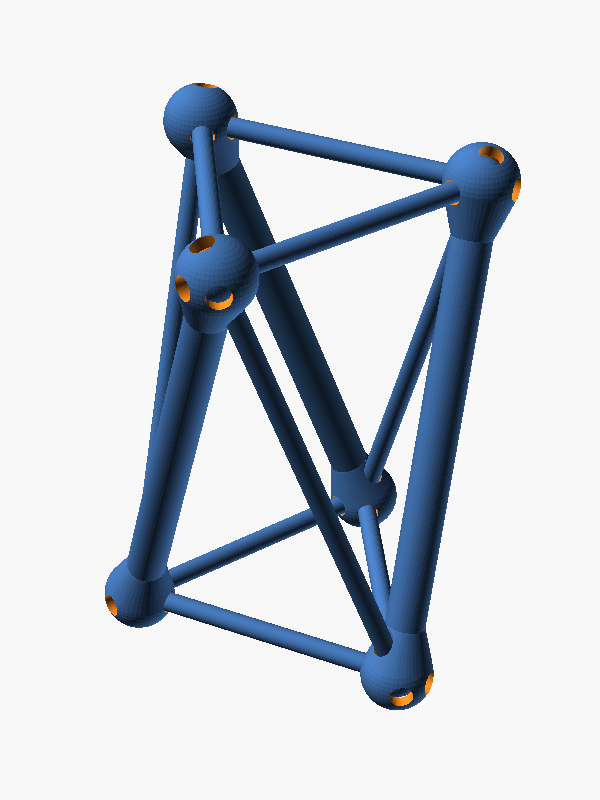
\includegraphics[width=\linewidth]{../figures/photos/cad-render.png}
    \label{fig:proto-cad}
  \end{subfigure}\hfill
  \begin{subfigure}[b]{0.54\linewidth}
    \centering
    \begin{tikzpicture}
      \node[anchor=south west,inner sep=0] (ph)
        {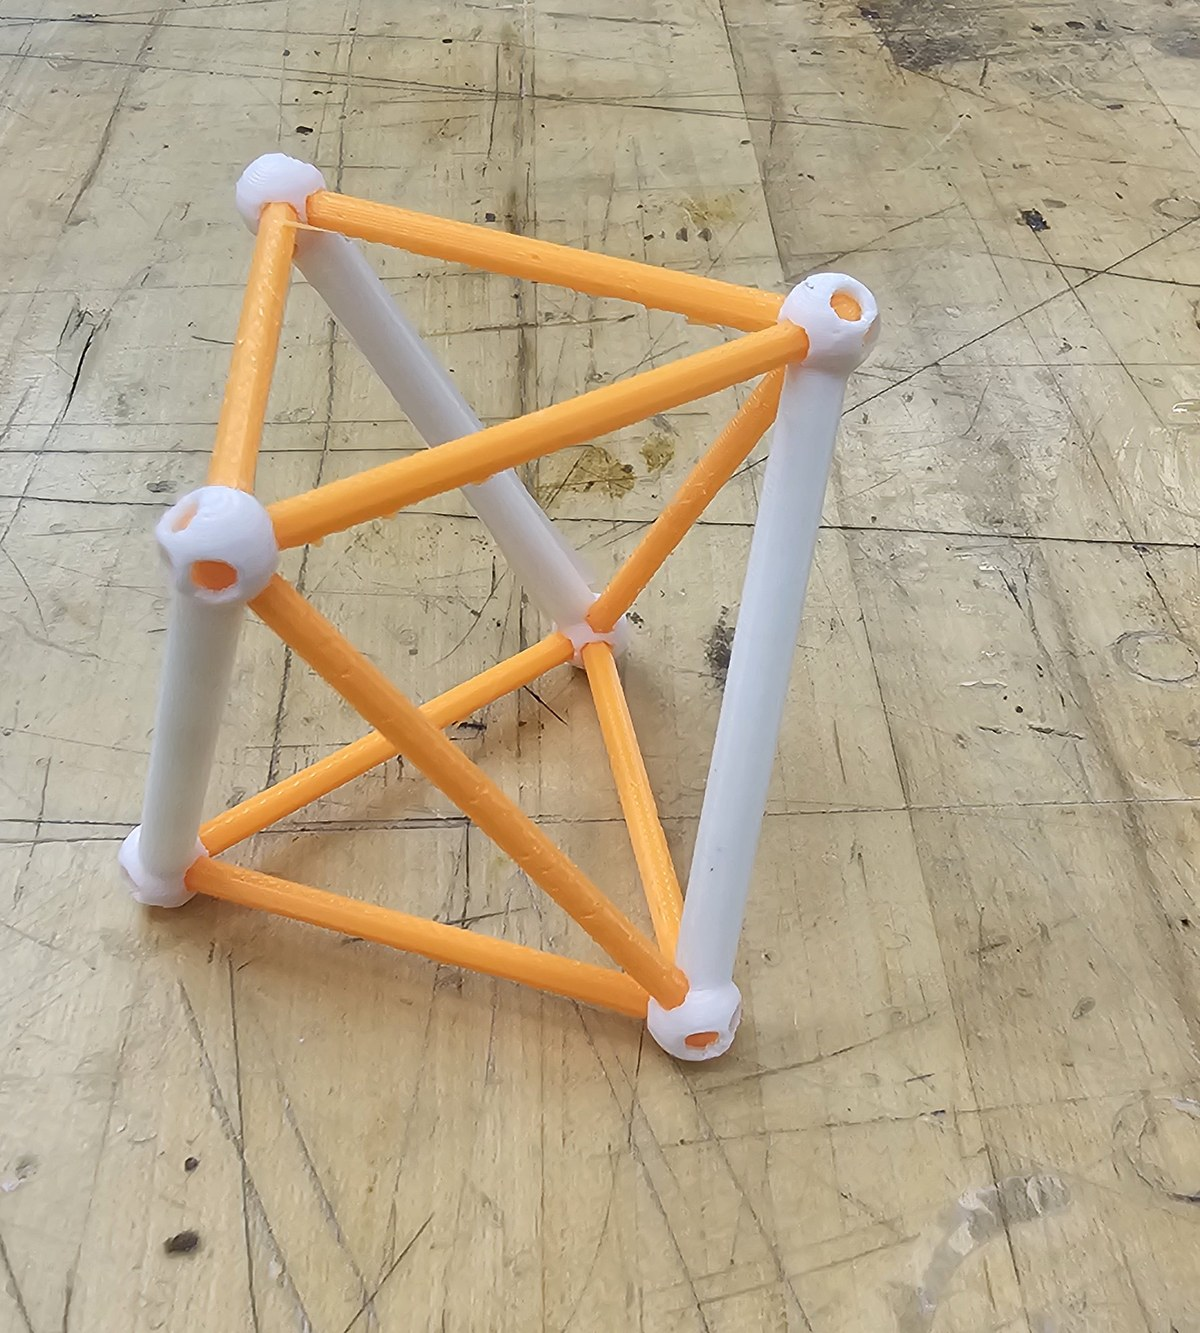
\includegraphics[width=\linewidth]{../figures/photos/printed-specimen.jpg}};
      \begin{scope}[x={(ph.south east)},y={(ph.north west)},
                    font=\sffamily\scriptsize]
        \tikzset{callout/.style={-{Latex[length=1.5mm]},line width=0.5pt,
                                 draw=red!75!black}}
        \tikzset{lab/.style={fill=white,fill opacity=0.85,text opacity=1,
                             inner sep=1pt,rounded corners=1pt}}
        \draw[callout] (0.74,0.95) node[lab,anchor=south]{$d_s$}
          -- (0.63,0.52);
        \draw[callout] (0.22,0.96) node[lab,anchor=south]{$d_t$}
          -- (0.34,0.70);
        \draw[{Latex[length=1.5mm]}-{Latex[length=1.5mm]},line width=0.5pt]
          (0.05,0.23) -- (0.05,0.85) node[lab,midway]{$H$};
      \end{scope}
    \end{tikzpicture}
    \label{fig:proto-print}
  \end{subfigure}
  \caption{Working $T_3$-prism prototype. \emph{(a)} Parametric OpenSCAD model
    whose base radius $R$, cell height $H$, twist angle $\theta$, strut diameter
    $d_s$, and cable diameter $d_t$ are the design variables of
    Table~\ref{tab:design-vars}. \emph{(b)} A representative dual-material print
    from the PR~\#35 print history (rigid PLA struts, here in white; tendon
    members in orange), with callouts marking the strut diameter $d_s$, a tendon
    (cable) diameter $d_t$, and the cell height $H$; the inter-plate twist
    $\theta$ is the relative rotation of the top and bottom node triangles, and
    the base radius $R$ sets their circumradius.}
  \label{fig:printed-prototypes}
\end{figure}

\subsection{Multi-Material Fabrication}
\label{sec:methods:fabrication}

Specimens are fabricated on a multi-material FDM printer using PLA for
the rigid struts and TPU for the soft tension elements.
Figure~\ref{fig:fab-workflow} summarizes the end-to-end fabrication and
characterization workflow, from parametric CAD through multi-material
slicing, dual-extrusion printing, post-processing, and mechanical
testing. Rather than
wrapping the struts in a continuous TPU skin, the current design anchors
the TPU tension elements \emph{inside} the ends of each PLA strut: the
cables converging at a given strut end are joined within the strut,
which acts as a rigid cage housing the junction, and the individual
tendons then exit through discrete outlets. This keeps the soft-rigid
interface in internal, compression-dominated pockets rather than at an
exposed overmolded surface. This construction effectively inverts the
material roles of Ye et~al.'s soft-skin-over-rigid-core
wrapping~\cite{ye2023multimaterial}: here a soft TPU core is captured within
a rigid PLA shell, so we cite that work only as a multi-material co-printing
precedent rather than as validation of the present junction. \todo{Quantitatively
verify the internal-anchoring junction strength against the PR~\#39 / PR~\#35
joint pull-out studies before making any cyclic-durability claim.} \todo{Document slicer profile
(layer height, infill, print speed, nozzle temperatures, retraction
settings) and validation prints used to characterize PLA-TPU interface
strength.}

\paragraph{Print platform and joint geometry} The working platform is
a Bambu Lab~H2D printer, which permits a single rigid-soft build
without filament swaps. Strut endpoints are tied to cables through
parametric joint geometries developed and ranked through a five-design
OpenSCAD study (anchor-bulb, dovetail, TPU-sleeve overmold,
eyelet-loop, and TPU-rebar variants); the working prototype uses a
dovetail joint (Design~B) with an anchor-bulb backup (Design~A) for
sensitivity studies, with a captive TPU core routed inside the PLA
shell to keep the soft tendon protected from layer-line failure at
the strut-to-cable transition. The full five-design comparison and the
selected junction are detailed in the Supplementary Information.\todo{Cite the
joint-design Phase-3 CAD review (Edison ANALYSIS \texttt{19e0c868}) and the
Phase-4 vision review (\texttt{e9a1f4cc}) once both are integrated into the
references.}

\paragraph{Supports for soft members} Because near-vertical TPU
tendons are otherwise unsupported during printing, automatic support
generation is disabled and supports are painted manually in the
slicer: PLA edge supports run along each tendon, with the
support-to-object clearance tightened from \SI{0.35}{mm} to
\SI{0.2}{mm} during tuning on the reference prism. Two support-removal
artifacts recur in the seed batch (surface stringing and, on two
articles, TPU strands pulled off bottom tendons during support
removal) and are logged per article in the print key (Supplementary
Information). An automated alternative (a lowered support-threshold
angle plus mesh-ray-cast narrowing pillars) was developed in parallel
and is documented in the Supplementary Information.

\paragraph{Moisture and nozzle management} TPU is hygroscopic, so the
soft filament is fed from a heated dry box held near \SI{8}{\percent}
relative humidity, logged per print. Midway through the seed batch the
TPU extruder developed a progressive flow taper (a partial clog,
compounded by a stray PLA fragment found inside the extruder); it was
resolved by a cold pull and by moving the TPU to a dedicated
high-flow \SI{0.6}{mm} nozzle, after which print quality was restored.
The affected and post-fix articles are identified in the print key so
that any nozzle-related covariate can be checked against the measured
objectives.

\begin{table}[ht]
  \centering
  \caption{Multi-material print parameters on the Bambu Lab~H2D,
    transcribed from the archived as-printed Bambu Studio project
    (\texttt{t3-prism-bo-batch.H2D-MM-PLAstruts-TPUcables.as-printed.3mf},
    Bambu Studio 2.7.1). Filaments are Bambu Lab PLA Basic (struts,
    support material) and Bambu Lab TPU~85A (tendons); the print
    profile is ``0.30\,mm Standard @BBL H2D 0.6 nozzle.'' The
    reporting structure follows the methods section of Ye
    et~al.~\cite{ye2023multimaterial}.}
  \label{tab:print-params}
  \small
  \setlength{\tabcolsep}{3pt}
  \begin{tabular}{@{}lcc@{}}
    \toprule
    Parameter & PLA (struts) & TPU 85A (tendons) \\
    \midrule
    Nozzle                             & \SI{0.6}{mm} & 0.4 then \SI{0.6}{mm} HF\textsuperscript{a} \\
    Nozzle temperature (\textdegree C) & 220 & 220 \\
    Bed temperature, profile (\textdegree C) & 55 & 35 \\
    Layer height / line width (mm)     & \multicolumn{2}{c}{0.30 / 0.62} \\
    Infill                             & 15\% grid, 2 walls & near-solid \\
    Outer / inner wall speed (mm/s)    & \multicolumn{2}{c}{200 / 300 (profile)} \\
    Filament drying                    & n/a & dry box, $\sim$8\% RH \\
    Build-plate type                   & \multicolumn{2}{c}{Textured PEI} \\
    Build orientation                  & \multicolumn{2}{c}{Vertical} \\
    Supports                           & \multicolumn{2}{c}{Manual painted tree supports, PLA} \\
    \bottomrule
  \end{tabular}\\[2pt]
  {\footnotesize \textsuperscript{a}The TPU side ran a standard
  \SI{0.4}{mm} nozzle until the mid-batch clog, then a dedicated
  high-flow (HF) \SI{0.6}{mm} nozzle; affected articles are flagged in
  the print key.}
\end{table}%
\todo{@achris0520 to confirm the physical nozzle hardware (the
  archived as-printed project records \SI{0.6}{mm} on both extruders,
  consistent with the post-fix state; the TPU side ran \SI{0.4}{mm}
  before the mid-batch nozzle change logged in the print key) and to
  supply filament lot numbers and drying duration, which the slicer
  archive does not record.}

\begin{figure*}[t]
  \centering
  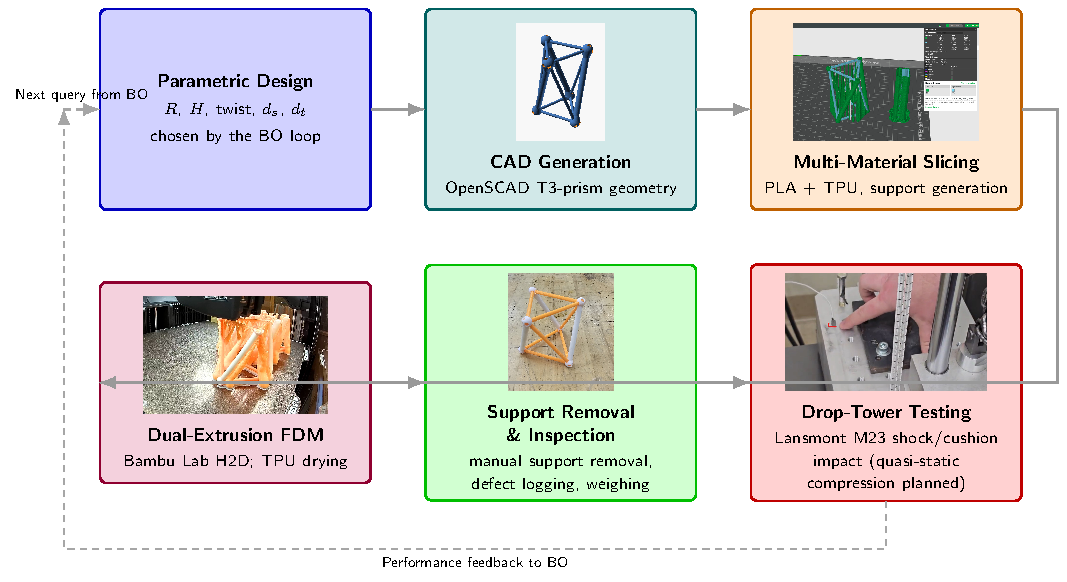
\includegraphics[width=\textwidth]{../figures/fab-workflow.pdf}
  \caption{Fabrication and characterization workflow for the multi-material
    tensegrity-inspired unit cells: design parameters drive parametric CAD,
    slicing with manually generated TPU supports, a single multi-material
    print on the Bambu Lab~H2D, post-processing and inspection, and
    mechanical testing. Node photographs are representative artifacts drawn
    from the project's build history: the OpenSCAD $T_3$-prism render
    (CAD), the dual-nozzle Bambu Studio slice with PLA on the left extruder
    and TPU on the right (slicing), an in-progress H2D print of the prism
    batch (FDM), an as-printed specimen (post-processing), and the
    bungee-assisted drop-tower base plate with accelerometer (testing).}
  \label{fig:fab-workflow}
\end{figure*}%

\subsection{Experimental Characterization}
\label{sec:methods:testing}

\paragraph{Drop-tower fixture} The primary characterization is
repeated drop-weight impact on a Lansmont Model~23 shock test system.
The printed specimen rides upright on the carriage plate, which is
raised \SI{60}{in} (\SI{1.524}{m}) along guide rails and released; the
plate lands on a single \SI{0.5}{in} Shore 60~OO polyurethane cushioning
sheet, which shapes the landing into a single sharp base pulse of
roughly \SI{1.6}{ms} duration. This impact-surface configuration was
selected by a blinded crossover experiment over three candidate mat
arrangements, and unlike a felt stack it does not measurably compact
over hundred-drop sessions. Rig health is monitored continuously
through the impact velocity change $\Delta v$ recovered from the base
accelerometer: over an uninterrupted 100-drop characterization session
the $\Delta v$ coefficient of variation was 0.54\% with no drift, and
every campaign session is checked against the healthy tower baseline
(details, including the within-session mat warm-up and recovery
pattern, in the Supplementary Information). One drop takes roughly
\SI{42}{s}, so a seed-batch characterization completes in about
ninety minutes per article and a later-batch session in about
fifteen.

\paragraph{Instrumentation and signal processing} A single-axis
piezoelectric accelerometer on the carriage plate records the base
input and triggers the acquisition; a triaxial accelerometer (Dytran
3133A4) seated in a printed pocket at the specimen's top vertex records
the transmitted response. The two base-capable channels were
cross-calibrated in place over fifteen co-located drops (ratio
$0.953 \pm 0.001$ at matched filtering), and the transducer settings
are archived with the data. Signals are captured at
\SI{1.25}{MHz} over a \SI{100}{ms} record with a \SI{2}{ms}
pre-trigger. All channels are low-pass filtered with the SAE~J211/1
channel-frequency-class (CFC) filters~\citep{saej211}, implemented from
the standard's published coefficients with the two-pass corner
frequency handled explicitly (a common implementation shortcut narrows
the passband by roughly 20\%, which we identified and corrected before
the campaign; all reported numbers use the corrected filter). CFC-180
is the reporting class for peak metrics, with CFC-1000 retained as a
higher-bandwidth diagnostic.

\paragraph{Per-article objectives and session protocol} Session
length evolved with the campaign's understanding of its own noise,
and the per-batch counts are stated here because they differ. Seed
sessions recorded 103 drops per article and contribute 101 stabilized
captures each (103 for one article, autv5r) after the first two drops
of each session are discarded as seating warm-up. A pre-campaign
variance study on the commissioning datasets put the statistical
minimum at five stabilized drops after two warm-ups, and the seed
sessions confirmed that the stabilized mean is insensitive to session
length: within-session per-drop CVs of 0.17 to 0.48\% with flat
post-warm-up trends, and a replay of the seed sessions truncated to
twenty drops leaves the transmissibility ranking of all eight tested
articles unchanged, with a worst-case mean shift of $+0.008$ against
design-to-design gaps of 0.007 to 0.087 and a per-drop standard
error still an order of magnitude below those gaps. Later sessions
were therefore shortened to about twenty drops per article: the
committed record lists 21 to 22 valid captures per batch-2 article
and 20 recorded drops per article in batches 3 and 4, against 101
valid captures per seed article, with the first two drops of every
session discarded as before (exact per-session counts are in the
archived per-drop records). The shortening cuts tower time per
article
from about ninety minutes to about fifteen while retaining roughly
four times the minimum stabilized-drop budget; a shorter session
simply enters the surrogate with a proportionally larger standard
error, which the model downweights. The second print-and-test pass
of batch 3
(Section~\ref{sec:results:batches}) subsequently confirmed that
seating and print variation, not session length, limit what a
session can claim, so the freed tower time goes to re-seats. Each
session yields two objectives, each reported as a stabilized mean
with the per-drop scatter quoted as one standard deviation; the
standard error of the mean is what enters the surrogate's noise model
(Section~\ref{sec:methods:bo}):
\begin{equation}
  \begin{aligned}
    t_{180} &\;=\; \frac{\max_t\,\lVert \mathbf{a}_{\mathrm{top}}(t)\rVert_{\mathrm{CFC180}}}
                        {\max_t\,\lvert a_{\mathrm{base}}(t)\rvert_{\mathrm{CFC180}}},\\
    E_{\mathrm{reb}} &\;=\; e_{\mathrm{reb}}\, m\, g\, h,
    \qquad
    e_{\mathrm{reb}} \;=\; \frac{g\, t_{\mathrm{second}}}{2\,\Delta v},
  \end{aligned}
  \label{eq:objectives}
\end{equation}
where $t_{180}$ is the CFC-180 filtered peak-acceleration ratio,
which we name once here and then call the \emph{transmissibility}
throughout: the peak magnitude of the triaxial top-vertex response
over the peak base input within the impact window. The term is used
in the shock-testing sense standard for cushioning and packaging
drop tests, a ratio of filtered peak accelerations across the
article under a single transient, not the steady-state
frequency-response function of vibration isolation: the two peaks
need not be simultaneous, the filter class is part of the
definition, and SAE~J211/1 is cited only for the impact-channel
filtering. Values above unity indicate the structure amplifies the
peak shock reaching its top vertex; values below unity indicate
attenuation. $E_{\mathrm{reb}}$ is a \emph{provisional
mass-weighted rebound score} with units of energy (millijoules per
drop): the dimensionless rebound fraction $e_{\mathrm{reb}}$ is
recovered from the ballistic timing of the top vertex's post-impact
hop~\citep{bernstein1977listening} ($t_{\mathrm{second}}$ is the time
to the second contact event and $\Delta v$ the measured base velocity
change), and it is scaled by each article's own weighed mass $m$ and
the drop height $h$. Two interpretive caveats are deliberate. The
ballistic reading of the second contact event has not yet been
validated against synchronized video, and $\Delta v$ is the base
plate's velocity change rather than a demonstrated incident relative
velocity, so $e_{\mathrm{reb}}$ is a rebound-timing score rather than
a coefficient of restitution; and because a strict restitution reading
would scale returned kinetic energy as the \emph{square} of a velocity
ratio, $E_{\mathrm{reb}}$ is a mass-aware ranking score that penalizes
designs (and grams) that throw more motion back at the payload, not a
measured rebound energy. The score is the campaign's second
objective through all four batches and remains a candidate to become
a constraint once validated
(Section~\ref{sec:discussion}). Using the mass-weighted form rather
than the bare fraction keeps the objective mass-aware: equal fractions
on articles of different printed mass are not equivalent outcomes for
a payload. Ringdown descriptors (the fitted natural frequency $f_n$,
260 to \SI{470}{Hz} for every article but one batch-4 design that
rings at \SI{764}{Hz}, and, where
the exponential fit passes an $r^2 \ge 0.85$ gate, a damping ratio
$\zeta$) are recorded per drop as print-health and prestress
diagnostics~\citep{ashwear2014natural} but are not campaign objectives.
The within-session per-drop CV of $t_{180}$ spans 0.06 to 2.0\%
across the campaign's 35 articles (0.17 to 0.48\% in the seed
batch). These
values describe repeated drops of the same physical article in one
seating and do not estimate print-to-print or seating-to-seating
repeatability; serial dependence among drops may also make
$s/\sqrt{n_{\mathrm{drops}}}$ optimistic. Two replication
measurements bound what a single session can claim: the seed
attenuator re-measured across a day and an independent re-seat
agreed to 0.13\%, while a full second print-and-test pass of the
batch-3 plate showed same-design shifts with a median of $+1.2\%$
and heavy tails (Section~\ref{sec:results:batches}). The campaign
therefore adopted a between-seat replication rule: a single-seating
value that would drive a decision (a batch extreme, a claimed
attenuator, a front membership) requires confirmation on an
independent re-seat before it is treated as a design property. A
mechanism-oriented trace figure (processed
deceleration response with event markers keyed to synchronized video
frames) will be generated from archived campaign captures once the
event labels can be supported by synchronized measurements; no such
figure is shown here because none of the required event
synchronization has yet been performed.

\paragraph{Planned quasi-static extension} The drop test loads the
specimens in their elastic regime (the crush lasts 1 to \SI{3}{ms} and
the article recovers), so crush-energy metrics such as specific energy
absorption (SEA) and compaction efficiency are not recoverable from
these captures by any reprocessing. A quasi-static compression
campaign on a benchtop load frame (BYU CB~123 Instron, with a
low-range load cell appropriate to the expected cell stiffness)
is planned to supply the complementary crush metrics
\begin{equation}
  \mathrm{SEA} \;=\; \frac{1}{m}\!\int_{0}^{\delta_d}\! F(\delta)\,
  \mathrm{d}\delta,
  \qquad
  \eta_c \;=\; \frac{\int_{0}^{\delta_d}\! F(\delta)\,\mathrm{d}\delta}{F_{\max}\,\delta_d},
\end{equation}
with the densification displacement $\delta_d$ taken at the maximum of
the energy-absorption efficiency curve and $F_{\max}$ the peak force
within $[0,\delta_d]$, following the canonical cellular-solid
treatments~\citep{gibson1997cellular, avalle2001characterization,
tan2005dynamic, michailidis2011establishment} and mirroring the
quasi-static protocol of Pajunen et~al.~\citep{pajunen2019design}.
These metrics are reported as a complementary characterization of
selected designs rather than as objectives of the drop-tower campaign.
Slip resistance and traction at the specimen-to-floor interface,
governed by the tip geometry rather than the internal architecture,
follow ISO 11334-4~\citep{iso11334-4} for walking-aid tips and are out
of scope for the present axial-impact study.

\paragraph{Complementary data streams} High-speed video
(\SI{959}{fps}, three clips per specimen) supplements the
accelerometer data. The camera cannot resolve the millisecond-scale
impact pulse (one to two frames), so the division of labor is
explicit: the accelerometer channels produce the objectives, and video
documents the post-impact rebound and recovery. Synchronized
laser-Doppler vibrometry is reserved for follow-up characterization of
selected designs.

\subsection{Experiment-Driven Bayesian Optimization Loop}
\label{sec:methods:bo}

The optimization loop maintains a Gaussian-process (GP) surrogate over
the design space defined in
Section~\ref{sec:methods:parameterization}. After each round of
physical experiments, the surrogate is refit and an acquisition
function is maximized to recommend the next batch of designs to
fabricate. The campaign is posed as a two-objective minimization:
simultaneously minimize the transmissibility $t_{180}$
and the per-drop rebound energy $E_{\mathrm{reb}}$ of
Eq.~\eqref{eq:objectives}. Both objectives serve the same payload:
$t_{180}$ bounds the peak shock it feels during the impact, and
$E_{\mathrm{reb}}$ penalizes the motion thrown back into it afterward.
The seed data showed an apparent trade-off driven substantially by
the single strongest attenuator, not statistically resolved at seven
mapped articles (Spearman $\rho = -0.39$, $p = 0.38$;
Section~\ref{sec:discussion}); the measured front after four batches
is nondegenerate (its members span both axes), and the rebound axis
remains a candidate to become a constraint once its ballistic
reading is validated.
Implementation
uses the Ax platform~\citep{pmlr-v293-olson25a} over
BoTorch~\citep{balandat2020botorch}, with noisy expected hypervolume
improvement (qNEHVI)~\citep{daulton2021nehvi} as the multi-objective
acquisition. The $T_3$-prism search space is fully continuous,
including the process variables added in batch 3
(Table~\ref{tab:design-vars}), so no categorical
encoding is required; the mixed-search-space constructions
of~\citep{garridomerchan2020dealingwithcategorical} and the BOCS
combinatorial baseline~\citep{baptista2018bocs} remain the route for
the future connectivity-topology categorical rather than part of the
current loop. The input-noise-robust acquisition of Daulton
et~al.~\cite{daulton2022robust} and the evolution-guided constrained
variant of Low et~al.~\cite{low2024evolution} are held in reserve as
contingencies.

\paragraph{Surrogate and noise model} The surrogate is the fully
Bayesian sparse axis-aligned subspace model
(SAASBO)~\citep{eriksson2021saasbo}: a Mat\'ern-5/2 kernel with
automatic relevance determination whose length scales carry strong
sparsity-inducing priors and are marginalized by Markov-chain Monte
Carlo (NUTS) rather than point-estimated; every refit in the
campaign, through the batch-4 ingestion, uses this model with qNEHVI
on top (Ax 0.4 for the early rounds, Ax~0.5.0 from the batch-3
refit). We retain SAASBO even though the
dimensionality is modest because marginalizing the hyperparameters
tends to improve uncertainty quantification at the very small sample
sizes of physical campaigns; the fitted model is audited each round
with leave-one-out cross-validation and length-scale-based
sensitivity diagnostics
(Section~\ref{sec:results}). Inputs are normalized to the unit cube
and outputs standardized. Observation noise is supplied per
observation as a fixed variance: for $t_{180}$ the squared standard
error of the stabilized mean,
$\sigma_t^2 = s_{\mathrm{drop}}^2 / n_{\mathrm{drops}}$, and for the
rebound score the drop-scatter term plus the propagated
print-to-print mass scatter,
$\sigma_E^2 = \sigma_{E,\mathrm{drops}}^2 +
(\partial E_{\mathrm{reb}}/\partial m)^2 \sigma_m^2$ with
$\sigma_m = \SI{0.457}{g}$ measured from the one design printed in
triplicate; a shorter session enters with a proportionally larger
standard error. The estimand this noise model implies is the
response of the tested article in its seating, not of a freshly
printed article at the same design: an independent adversarial
review (Section~\ref{sec:discussion}) argued the decision-relevant
target is the latter, and the campaign's response is the measured
replication evidence of Section~\ref{sec:results:batches} (a full
second print-and-test pass of one batch) together with the
between-seat replication rule, rather than an inflated per-article
noise term. SAASBO is the
prespecified surrogate; we make no claim that it outperforms
a standard single-task GP at this dimensionality and sample size,
and the planned head-to-head calibration comparison against a
point-estimated GP with the same kernel remains future work.

\paragraph{Mass treatment} Because the constant \emph{solid}-mass
projection of batches 1 and 2 does not hold printed grams constant
(Section~\ref{sec:methods:parameterization}), printed mass correlates
with the shape variables in the seed batch ($r = 0.83$, $n = 7$,
dominated by the lightest article, against $t_{180}$). The loop
therefore makes mass explicit rather than pretending it away: the
rebound objective is expressed in absolute millijoules using each
article's weighed mass, so added grams are re-penalized through the
energy they deliver back to the payload, while $t_{180}$ deliberately
stays a ratio because payload peak acceleration is a damage criterion
that does not scale with specimen mass. The objective surrogates take
the design coordinates of Table~\ref{tab:design-vars} as their
inputs; printed mass is attached as a separately modeled
\emph{tracking metric}, so the model learns as-printed mass as a
function of the design coordinates and every recommendation reports a
predicted printed mass (the diagnostic refit behind
Fig.~\ref{fig:sensitivity} additionally includes printed mass as an
input, precisely to probe this confound). The calibrated
printed-mass model of the Supplementary Information closed the loop
on this compromise: batches 3 and 4 hold \emph{printed} grams
constant, and the mass-transmissibility correlation across the 26
articles of batches 1 to 3 fell to $r = 0.07$, so the confound the
seed batch raised was broken by design rather than adjusted away in
analysis.

\paragraph{Budget and seeding} The seed batch is an $n = 9$ Sobol
draw with a recorded seed over the five-variable box, printed together
with the fixed reference prism (S0). Optimization proceeds in
sequential batches of $q = 9$ prints, sized to one build-plate
generation cycle. Three model-recommended batches are reported here
(Ax trials 10 to 18, 28 to 36, and 37 to 45; the numbering gap
records a superseded draft batch that was regenerated, before
printing, when the batch-level filament handling was simplified).
From batch 3 the four filament settings take one quasi-random point
per batch, formally the settings of that batch's best-predicted
article, so those axes are confounded with batch and are reported as
unidentified rather than learned. All random seeds,
the full experiment state, and the recommendation tables are recorded
per round; full computational reproducibility (the exact processing
pipeline and model settings) is carried by the campaign code, whose
archival release is a declared submission gate rather than a solved
item. Escalation to
trust-region BO (TuRBO)~\citep{eriksson2019turbo} is planned only if
per-member-diameter extensions push the design space well beyond the
present regime; a single-objective log-Expected-Improvement
run~\citep{ament2023logei} on $t_{180}$ is retained as a baseline for
quantifying the benefit of the multi-objective formulation. The
campaign code and recommended batches will be archived at a
Zenodo-minted DOI mirroring the GitHub repository.\todo{Insert the
Zenodo DOI and release version for the campaign code once the
repository snapshot is published.}

\subsection{Replicate Rank-Stability Study}
\label{sec:methods:rankstability}

The batch-3 second pass (Section~\ref{sec:results:batches}) showed
that a single article's measurement can move between seatings and
prints by more than the design signal separating neighboring
articles, which bounds any claim that one design outranks another. A
planned replicate study formalizes that bound by re-printing a
deliberately spread subset of the already-measured designs. Among
the campaign's in-sample designs, ranked by the current posterior's
predictions, we will select the best-predicted design, the
worst-predicted design, and one mid-pack (``run-of-the-mill'')
design, then print a nominal three fresh articles of each (the
repeat count, provisionally three, will be fixed when the print is
scheduled) and drop-test every article under the standard protocol
of Section~\ref{sec:methods:testing}, including the between-seat
replication rule. The question is whether the predicted ordering
survives fabrication and seating variation. With three designs the
exact permutation floor for a Spearman rank correlation is
$p = 1/6$, so no significance claim is available at this size;
the primary readout is instead the separation of the three designs'
repeat clusters relative to the within-design (print-to-print plus
seat-to-seat) scatter, reported alongside $\rho_s$ between the
predicted and measured orderings of each repeat. Clean separation
would support treating the campaign's rankings as design properties;
overlapping clusters would localize the ranking noise floor that the
batch-3 second pass could only bound. The reporting format is
specified in Table~\ref{tab:rank-stability}; entries and design IDs
will be added once the repeat articles are printed and tested.

\begin{table}[ht]
  \centering
  \caption{\emph{Placeholder (data pending).} Planned replicate
    rank-stability study: the best-, mid-, and worst-predicted
    in-sample designs, each re-printed as a nominal three fresh
    articles and drop-tested under the standard protocol. Entries
    will record each repeat's stabilized $t_{180}$, the
    within-design scatter, and the measured rank of each design's
    repeat cluster against its predicted rank.}
  \label{tab:rank-stability}
  \small
  \begin{tabular}{@{}llcccc@{}}
    \toprule
    Tier & Design & {Pred.\ $t_{180}$} &
    \multicolumn{3}{c}{$t_{180}$ (repeats 1 / 2 / 3)} \\
    \midrule
    Best  & \textit{TBD} & \textit{-} & \textit{-} & \textit{-} & \textit{-} \\
    Mid   & \textit{TBD} & \textit{-} & \textit{-} & \textit{-} & \textit{-} \\
    Worst & \textit{TBD} & \textit{-} & \textit{-} & \textit{-} & \textit{-} \\
    \bottomrule
  \end{tabular}
\end{table}%
\todo[inline,color=orange!30]{Populate Table~\ref{tab:rank-stability}
  once the repeat articles of the best-, mid-, and worst-predicted
  in-sample designs are printed and drop-tested; fix the repeat count
  (nominally three) and the design IDs when the print is scheduled.}

\subsection{Metal-Analog Validation}
\label{sec:methods:validation}

In the future we plan a validation campaign that tests whether the
rankings learned on the printed PLA/TPU specimens generalize beyond
the as-printed polymer system, by reproducing a subset of the
$T_3$-prism designs as
\emph{metal analogs} built from hollow aluminum rods (compression
members) and stainless-steel threaded cables (tension members), using
the same $R$, $H$, $\theta$, and member-diameter parameterization.
Rather than fabricating only the top-ranked geometries, we
deliberately span the predicted performance range: a few designs the
surrogate predicts to be \emph{worst}-performing, a few
\emph{mediocre}, and a few \emph{best}-performing are each built in
both material systems. Comparing the measured ordering of the
PLA/TPU specimens against their hollow-aluminum/stainless-steel
counterparts probes whether both systems preserve the same
rank ordering of impact performance. We treat this as a
\emph{planned, exploratory} comparison rather than a preregistered
validation: the deformation modes, joint compliance,
friction, pretension behavior, and strain-rate sensitivity all differ
between the PLA/TPU and aluminum/steel systems, so agreement is not
expected a priori, and the protocol details that would let the
comparison distinguish geometric rank transfer from material-system
and mass confounds (aluminum alloy and temper, tube wall thickness,
cable construction, joint hardware and torque, article and payload
masses, replicate count, and tie-handling rules) remain to be fixed
and will be tabulated before any metal article is built. The intended
rank statistic is the Spearman rank-correlation coefficient $\rho_s$
between the two
material systems' orderings of the primary campaign metric ($t_{180}$
under the identical drop protocol), reported with an exact permutation
test, with the provisional rebound score
$E_{\mathrm{reb}}$ and, once the quasi-static extension runs, SEA
reported as secondary rankings. Rank agreement would be preliminary
evidence consistent with transfer; disagreement would not isolate
which material or joint difference caused the change.
The planned reporting format is specified in
Table~\ref{tab:metal-validation}; the table entries and the specimen
photographs of Fig.~\ref{fig:metal-validation} will be added after
fabrication and testing.

\begin{table}[ht]
  \centering
  \caption{\emph{Placeholder (data pending).} Planned rank-ordering
    validation: representative $T_3$-prism designs predicted to be
    worst-, mid-, and best-performing, each fabricated as a printed
    PLA/TPU specimen and as a hollow-aluminum-rod / stainless-steel-cable
    metal analog. Entries record the measured performance metric
    ($t_{180}$ under the identical drop protocol, with the provisional
    rebound score secondary) and the resulting rank within each
    material system; rank agreement would be preliminary evidence
    consistent with transfer, while disagreement would not isolate
    which material or joint difference caused the change.}
  \label{tab:metal-validation}
  \begin{tabular}{@{}llcc@{}}
    \toprule
    Predicted tier & Design ID & PLA/TPU (rank) & Al/SS (rank) \\
    \midrule
    Worst    & \textit{D-w1} & \textit{-} & \textit{-} \\
    Worst    & \textit{D-w2} & \textit{-} & \textit{-} \\
    Mediocre & \textit{D-m1} & \textit{-} & \textit{-} \\
    Mediocre & \textit{D-m2} & \textit{-} & \textit{-} \\
    Best     & \textit{D-b1} & \textit{-} & \textit{-} \\
    Best     & \textit{D-b2} & \textit{-} & \textit{-} \\
    \bottomrule
  \end{tabular}
\end{table}%
\todo[inline,color=orange!30]{Populate Table~\ref{tab:metal-validation}
  with measured metrics and ranks once the metal-analog validation
  specimens (hollow Al rods + stainless-steel threaded cables) and their
  PLA/TPU equivalents have been built and tested.}

\figplaceholder{metal-validation}{Assembled validation specimens for
  each predicted performance tier (worst / mediocre / best), shown as
  printed PLA/TPU builds alongside their hollow-aluminum-rod and
  stainless-steel-threaded-cable metal analogs, with callouts marking
  the aluminum compression members, the threaded steel tension cables,
  and the strut-end cable anchors. Photographs to be added once the
  specimens are fabricated.}

% =============================================================================
\section{Results}
\label{sec:results}
% =============================================================================

\subsection{Seed-Batch Measurements}
\label{sec:results:seed}

All nine Sobol specimens and the reference prism were printed and
declared acceptable to test. Nine articles (seven mapped Sobol
designs, the reference prism, and one article whose design mapping
is unconfirmed) completed seed characterization sessions, totaling
over 900 clean captures within a project-wide history of more than
4{,}000 instrumented drops; the two remaining seed designs (specs 03
and 06) were printed, but their drop sessions are absent from the
campaign record and they do not enter any fit or figure.
Table~\ref{tab:seed-results} reports the
stabilized objectives. Three findings frame the batch. First, the
measured $t_{180}$ spans 0.893 to 1.062: six of nine tested articles
\emph{amplify} the peak shock reaching the top vertex (means above
unity), two sit marginally below unity (0.997 and 0.980), and one
tested article (the print of Sobol spec~01, the thick-strut,
thin-cable, high-twist corner of the batch) had a mean $t_{180}$ of
0.893, indicating peak attenuation under the tested condition. This
article's attenuation later reproduced across an independent re-seat
to 0.13\%, the campaign's positive control for the replication rule
of Section~\ref{sec:methods:testing}.
Across the tested articles, $t_{180}$ spans 0.169 (18.9\% of
the observed minimum). This between-article range far exceeds the
0.17 to
0.48\% within-session per-drop CV, but one mechanically tested
article per geometry does not permit separation of geometry effects
from print-to-print variation or other fabrication covariates.
Second, the objectives show an
apparent trade-off in this sample: the best attenuator carries the
largest rebound score (13.9~mJ per drop), so the observed front is
nondegenerate, although the trade-off is driven substantially by that
single article and is not statistically resolved at this sample size
(Section~\ref{sec:discussion}). Third, among the eight mapped
articles with weighed masses, printed mass and $t_{180}$ showed a
large sample
correlation ($r = 0.82$, $n = 8$). The association is confounded with
the design coordinates and is highly sensitive to the lightest
article ($r = 0.26$ when 6lhxfy is omitted); it is not evidence of a
causal mass effect. It nonetheless motivated the mass-aware objective
formulation of Section~\ref{sec:methods:bo}, and the
constant-printed-mass batches later broke the confound outright
(Section~\ref{sec:results:audits}). Figure~\ref{fig:seed-designs} renders
the seed geometries to a common scale, showing how widely the
constant-mass box spans aspect ratio, member sizing, and twist.

\begin{figure}[t]
  \centering
  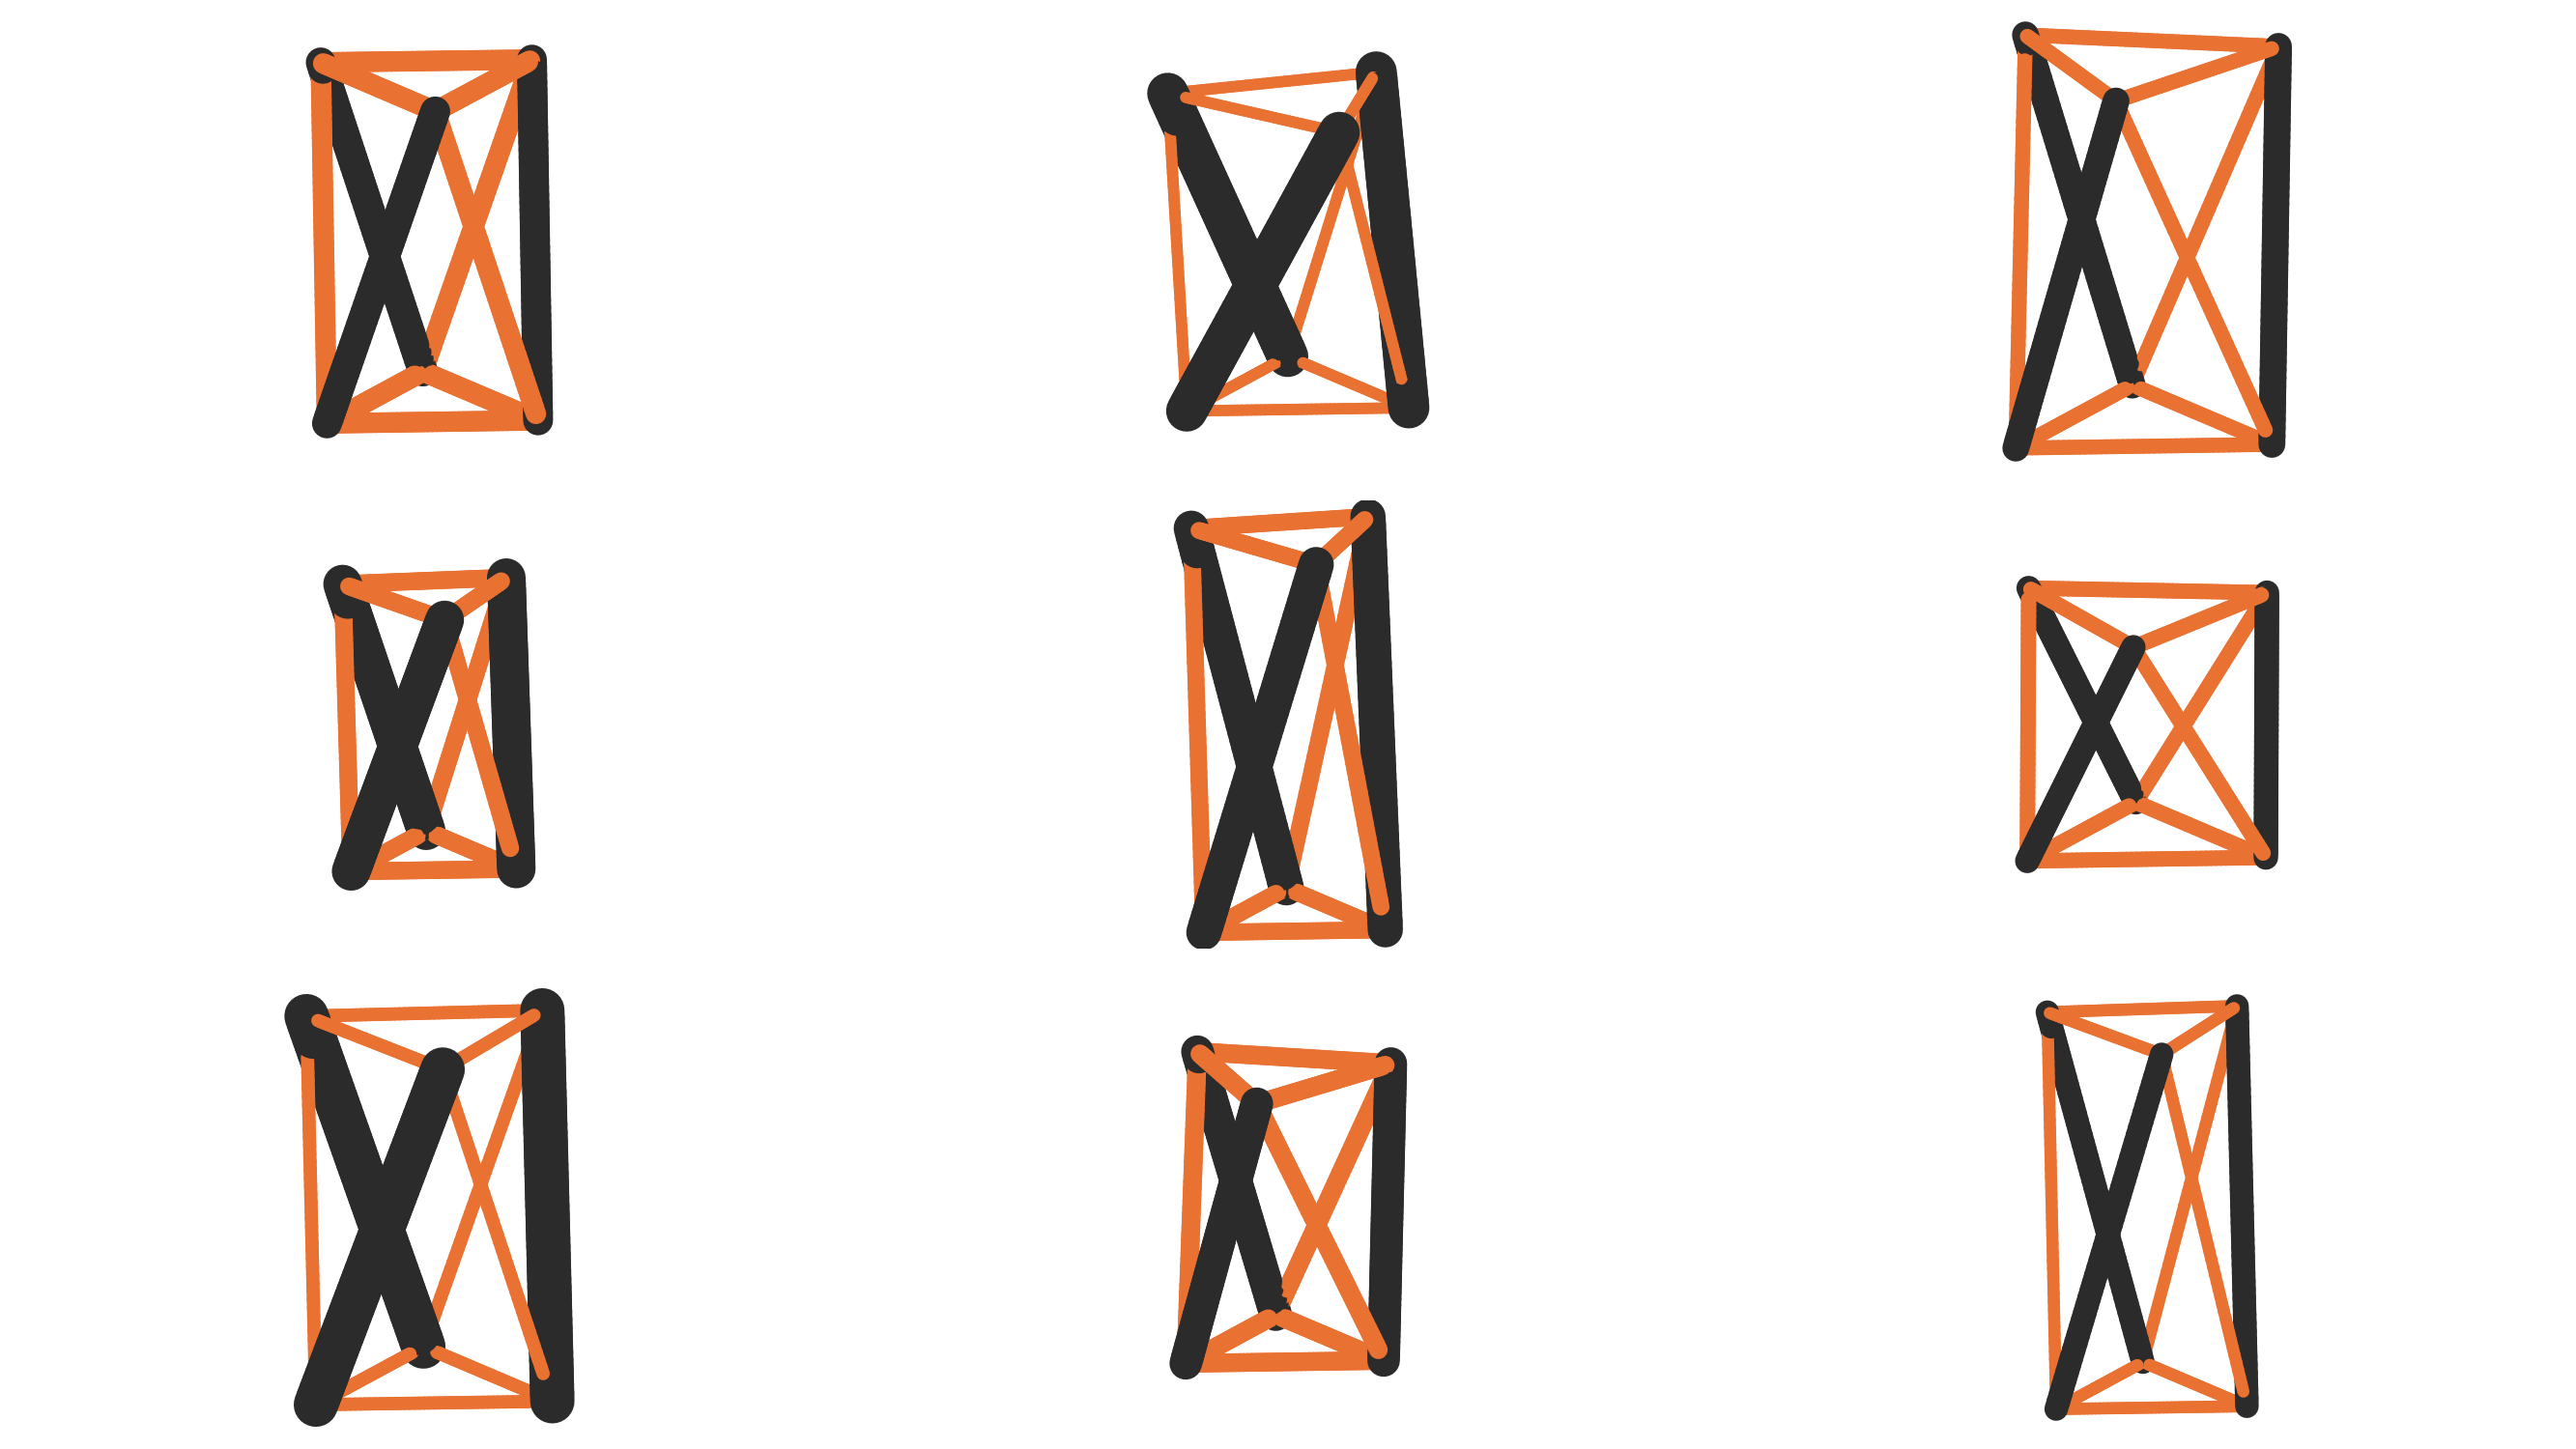
\includegraphics[width=\linewidth]{../figures/bo/fig-seed-designs.png}
  \caption{The nine seed geometries rendered to a common millimeter
    scale (rigid PLA struts in black, TPU tendons in orange). Every
    rendering corresponds to a physically printed article in the seed
    campaign.}
  \label{fig:seed-designs}
\end{figure}

\begin{table*}[t]
  \centering
  \caption{Seed-batch drop-tower results: 101 stabilized captures per
    article (103 for autv5r) at \SI{60}{in} onto the standardized
    polyurethane surface, CFC-180 filtering, counted after the first
    two warm-up drops of each session were discarded. Means $\pm$ one
    standard deviation over the stabilized drops; rows are ordered by
    $t_{180}$. $E_{\mathrm{reb}}$ uses each
    article's weighed mass per Eq.~\eqref{eq:objectives}. The ringdown
    frequency $f_n$ is a print-health descriptor, not an objective.
    A dash denotes a quantity that cannot be computed from the
    available record: article \textit{amdjwm} lacks a weighed mass and
    a confirmed design mapping (it is excluded from the surrogate fit
    and from all mass-dependent quantities), and no accepted $f_n$
    estimate is available for \textit{bag26v} or \textit{ajhby6}.
    Specs 03 and 06 were printed but have no drop sessions in the
    campaign record.}
  \label{tab:seed-results}
  \small
  \begin{tabular}{@{}llS[table-format=2.2]S[table-format=1.4]@{\,$\pm$\,}S[table-format=1.4]S[table-format=2.1]S[table-format=3.0]@{}}
    \toprule
    Design & Article & {Mass (g)} & \multicolumn{2}{c}{$t_{180}$} &
    {$E_{\mathrm{reb}}$ (mJ)} & {$f_n$ (Hz)} \\
    \midrule
    Spec 01 & 6lhxfy & 18.50 & 0.8931 & 0.0042 & 13.9 & 368 \\
    (unmapped) & amdjwm & {-} & 0.9805 & 0.0025 & {-} & 455 \\
    Spec 05 & 6nheas & 21.73 & 0.9970 & 0.0032 & 13.1 & 322 \\
    S0 ref. & bpx68c & 20.23 & 1.0111 & 0.0024 & 6.2 & 468 \\
    Spec 07 & ajhby6 & 20.53 & 1.0127 & 0.0038 & 6.1 & {-} \\
    Spec 00 & 9hhbkp & 21.62 & 1.0183 & 0.0017 & 6.9 & 364 \\
    Spec 04 & nvxsrv & 20.66 & 1.0275 & 0.0044 & 8.2 & 294 \\
    Spec 02 & autv5r & 22.04 & 1.0404 & 0.0035 & 8.8 & 386 \\
    Spec 08 & bag26v & 21.42 & 1.0616 & 0.0051 & 7.7 & {-} \\
    \bottomrule
  \end{tabular}
\end{table*}

\subsection{Model-Recommended Batches and Replication}
\label{sec:results:batches}

Table~\ref{tab:batch-results} reports the stabilized objectives for
the three model-recommended batches, and
Fig.~\ref{fig:front-evolution} overlays every measured article with
the non-dominated front after each batch (Pareto membership is
evaluated over articles with both objectives; the unmapped seed
article amdjwm is omitted because its missing weighed mass prevents
computing $E_{\mathrm{reb}}$). Dominated hypervolume, evaluated at
the fixed reference point $(t_{180}, E_{\mathrm{reb}}) =
(1.35, \SI{15}{mJ})$, grew from 3.155 after the seed batch to 3.969
after batch 2 ($+25.8\%$), 4.007 after batch 3 ($+0.9\%$), and 5.195
after batch 4 ($+29.7\%$): a 65\% total gain over the seed front. No
budget-matched quasi-random physical baseline has been run, so the
comparison the data support is against the campaign's own Sobol
seed: after batch 4, every member of the combined front (corny7,
corny6, drran5, drran3, r2d2c6) is a model-recommended design, and
the last seed article left the front when the batch-4 record
dominated it outright.

\paragraph{Batch 2 (Ax trials 10 to 18)} The first recommended batch
was generated from the seed fit and printed under the
constant-solid-mass projection, so its printed masses still spread
widely (17.91 to \SI{23.47}{g}; a regenerated constant-printed-mass
recommendation set is archived alongside the as-printed one, and the
two must not be conflated). The batch grew the front almost entirely
on the rebound axis: r2d2c6's \SI{4.1}{mJ} per drop is the lowest
rebound on record and still stands, and four batch-2 articles joined
the front. On the transmissibility axis the batch humbled its own
forecasts: the archived posterior predictions sat below the
measurements for nine of nine articles (mean absolute percentage
error 14.4\%; worst case r2d2c3, predicted 0.910, measured 1.334,
the strongest amplifier in the campaign record). That nine-of-nine
optimism widened the refit posterior for every batch that followed.

\paragraph{Batch 3 (Ax trials 28 to 36)} The first batch at constant
\emph{printed} mass (19.24 to \SI{20.06}{g}, CV 1.7\%) and the first
with the infill and filament axes active
(Section~\ref{sec:methods:parameterization}). It filled the knee of
the front rather than growing the box ($+0.9\%$ hypervolume; three
articles joined), and the recalibrated posterior held: eight of nine
articles measured within 0.3 posterior standard deviations of their
predictions (MAPE 3.8\%). The batch also delivered the campaign's
sharpest single surprise in both directions: the best-predicted
design (trial 32, predicted 1.020) measured 1.251, the strongest
amplification then on record, while the batch's only attenuator
(drran8, 0.980, drift-flagged, provisional) was its only twisted
design.

\paragraph{Batch 4 (Ax trials 37 to 45)} The acquisition split the
batch between the wide, high-twist, thin-cable family it had been
steering toward since batch 2 and a previously unvisited tall,
low-twist corner. The wide family delivered: four of nine articles
attenuate, and corny7, the batch's best-predicted design (trial 37,
predicted $0.934 \pm 0.13$), measured $t_{180} = 0.8031 \pm 0.0025$,
the strongest attenuation in the program, 10\% below the best seed
article and 21\% below the reference prism, at a mid-pack
\SI{9.4}{mJ} rebound; it dominates the seed attenuator on both
objectives (Fig.~\ref{fig:batch4-pred-vs-meas}). Within the
attenuating family the frozen predictions ranked the four
measurements perfectly (Spearman $\rho = +1.0$; $0.82$ across all
nine, where the five amplifier predictions span only 0.9\% and so
carry no ordering signal), batch MAPE was 6.0\%, and no article left
its predictive band by more than one standard deviation (the record
itself beat its band by 1.0 standard deviation in the good
direction). Per the between-seat replication rule, the batch-4
attenuation values, including the record, are single-seating
measurements whose re-seat confirmations are scheduled; one session
(corny5) carries a drift flag and its mean is provisional, and
another (corny6) was erratic (per-drop CV 2.0\%) but attenuates
under any reading of its record.

\paragraph{Replication: a second pass of batch 3} The batch-3 plate
was printed a second time (nine design replicates, the reprint
weighing \SI{0.27}{g} heavier article for article on average) and
the second set was drop-tested under the identical protocol, 360
drops across the two passes. Neither extreme of the first pass
recurred. Under \emph{any} pairing of the blinded session labels,
the design that measured 1.251 re-measured at most 1.090 (a drop of
at least 13\%) and the 0.980 attenuator re-measured at least 1.011,
so batch 3 contains no reproducibly attenuating design; under the
best-fit pairing, the same-design shifts have median $+1.2\%$, five
of nine fall inside the previously characterized $\pm 2.2\%$ re-seat
envelope, and the tails reach $-13.8\%$. The two passes cannot
separate seating effects from print-to-print differences, but the
methodological conclusion does not depend on that split: the 1.251
session had passed every within-session stability check (per-drop CV
0.77\%, no drift), so \emph{within-session stability does not
certify a measurement as a design property}. The between-seat
replication rule of Section~\ref{sec:methods:testing} was adopted in
response, the seed attenuator's 0.13\% agreement across an
independent re-seat shows that genuine attenuation does reproduce,
and a broadband seat gauge (the ratio of CFC-1000 to CFC-180
transmissibility; healthy sessions read 1.00 to 1.07) now
accompanies the rule as an advisory: every large same-design shift
observed so far carried a gauge reading of at least 1.15 in one of
its seatings, and all four batch-4 attenuators gauge healthy (0.98
to 1.06).

\begin{table*}[t]
  \centering
  \caption{Model-recommended batch results under the protocol and
    reporting conventions of Table~\ref{tab:seed-results} (CFC-180,
    stabilized means $\pm$ one standard deviation; about twenty
    drops per article against the seed batch's 101, with exact
    per-session counts in the archived per-drop records; rows
    ordered by $t_{180}$ within each batch).
    $E_{\mathrm{reb}}$ uses each article's weighed mass per
    Eq.~\eqref{eq:objectives}. ``Pred.'' is the posterior-mean
    $t_{180}$ archived when the batch was recommended, before any of
    its articles were tested. Batch-2 articles were projected to
    constant solid mass; batches 3 and 4 to constant printed mass
    (\SI{20.23}{g}). Flags follow the session record: $\dagger$
    marks a transmissibility-drift-flagged session whose mean is
    provisional, and $\ddagger$ marks the erratic corny6 session
    (per-drop CV 2.0\%).}
  \label{tab:batch-results}
  \small
  \begin{tabular}{@{}clcS[table-format=2.2]S[table-format=1.4]@{\,$\pm$\,}S[table-format=1.4]S[table-format=2.1]S[table-format=1.3]@{}}
    \toprule
    Batch & Article & Trial & {Mass (g)} & \multicolumn{2}{c}{$t_{180}$} &
    {$E_{\mathrm{reb}}$ (mJ)} & {Pred.\ $t_{180}$} \\
    \midrule
    2 & r2d2c7 & 15 & 18.51 & 0.9484 & 0.0008 & 12.2 & 0.905 \\
    2 & r2d2c1 & 13 & 19.38 & 0.9942 & 0.0021 & 6.0 & 0.948 \\
    2 & r2d2c2$^\dagger$ & 12 & 17.96 & 1.0411 & 0.0154 & 5.6 & 0.926 \\
    2 & r2d2c9 & 10 & 17.91 & 1.0530 & 0.0035 & 5.8 & 0.873 \\
    2 & r2d2c6 & 14 & 19.11 & 1.0548 & 0.0042 & 4.1 & 0.953 \\
    2 & r2d2c8 & 17 & 19.98 & 1.0704 & 0.0116 & 7.9 & 0.955 \\
    2 & r2d2c5 & 18 & 23.47 & 1.1516 & 0.0040 & 6.7 & 0.987 \\
    2 & r2d2c4 & 11 & 19.33 & 1.1847 & 0.0076 & 6.4 & 0.885 \\
    2 & r2d2c3 & 16 & 18.63 & 1.3337 & 0.0117 & 5.6 & 0.910 \\
    \midrule
    3 & drran8$^\dagger$ & 35 & 19.32 & 0.9804 & 0.0051 & 11.2 & 1.039 \\
    3 & drran1 & 36 & 19.31 & 1.0326 & 0.0016 & 18.1 & 1.051 \\
    3 & drran4 & 29 & 19.92 & 1.0344 & 0.0017 & 9.1 & 1.032 \\
    3 & drran2 & 33 & 19.33 & 1.0345 & 0.0006 & 11.8 & 1.056 \\
    3 & drran5 & 28 & 19.88 & 1.0373 & 0.0024 & 5.0 & 1.059 \\
    3 & drran3 & 31 & 19.92 & 1.0389 & 0.0012 & 4.2 & 1.043 \\
    3 & drran9 & 30 & 19.34 & 1.0425 & 0.0009 & 5.2 & 1.058 \\
    3 & drran6 & 34 & 19.24 & 1.0471 & 0.0040 & 4.8 & 1.065 \\
    3 & drran7 & 32 & 20.06 & 1.2513 & 0.0096 & 8.2 & 1.020 \\
    \midrule
    4 & corny7 & 37 & 19.62 & 0.8031 & 0.0025 & 9.4 & 0.934 \\
    4 & corny9 & 43 & 19.46 & 0.8766 & 0.0036 & 18.1 & 0.942 \\
    4 & corny6$^\ddagger$ & 41 & 19.45 & 0.9106 & 0.0181 & 5.7 & 0.943 \\
    4 & corny8 & 39 & 19.64 & 0.9535 & 0.0025 & 17.5 & 0.954 \\
    4 & corny1 & 42 & 20.20 & 1.0459 & 0.0029 & 8.7 & 1.010 \\
    4 & corny4 & 44 & 20.56 & 1.0475 & 0.0025 & 4.3 & 1.013 \\
    4 & corny3 & 45 & 20.15 & 1.0705 & 0.0013 & 8.8 & 1.004 \\
    4 & corny2 & 38 & 20.21 & 1.0846 & 0.0030 & 9.2 & 1.008 \\
    4 & corny5$^\dagger$ & 40 & 20.58 & 1.0876 & 0.0099 & 8.5 & 1.012 \\
    \bottomrule
  \end{tabular}
\end{table*}

\begin{figure*}[t]
  \centering
  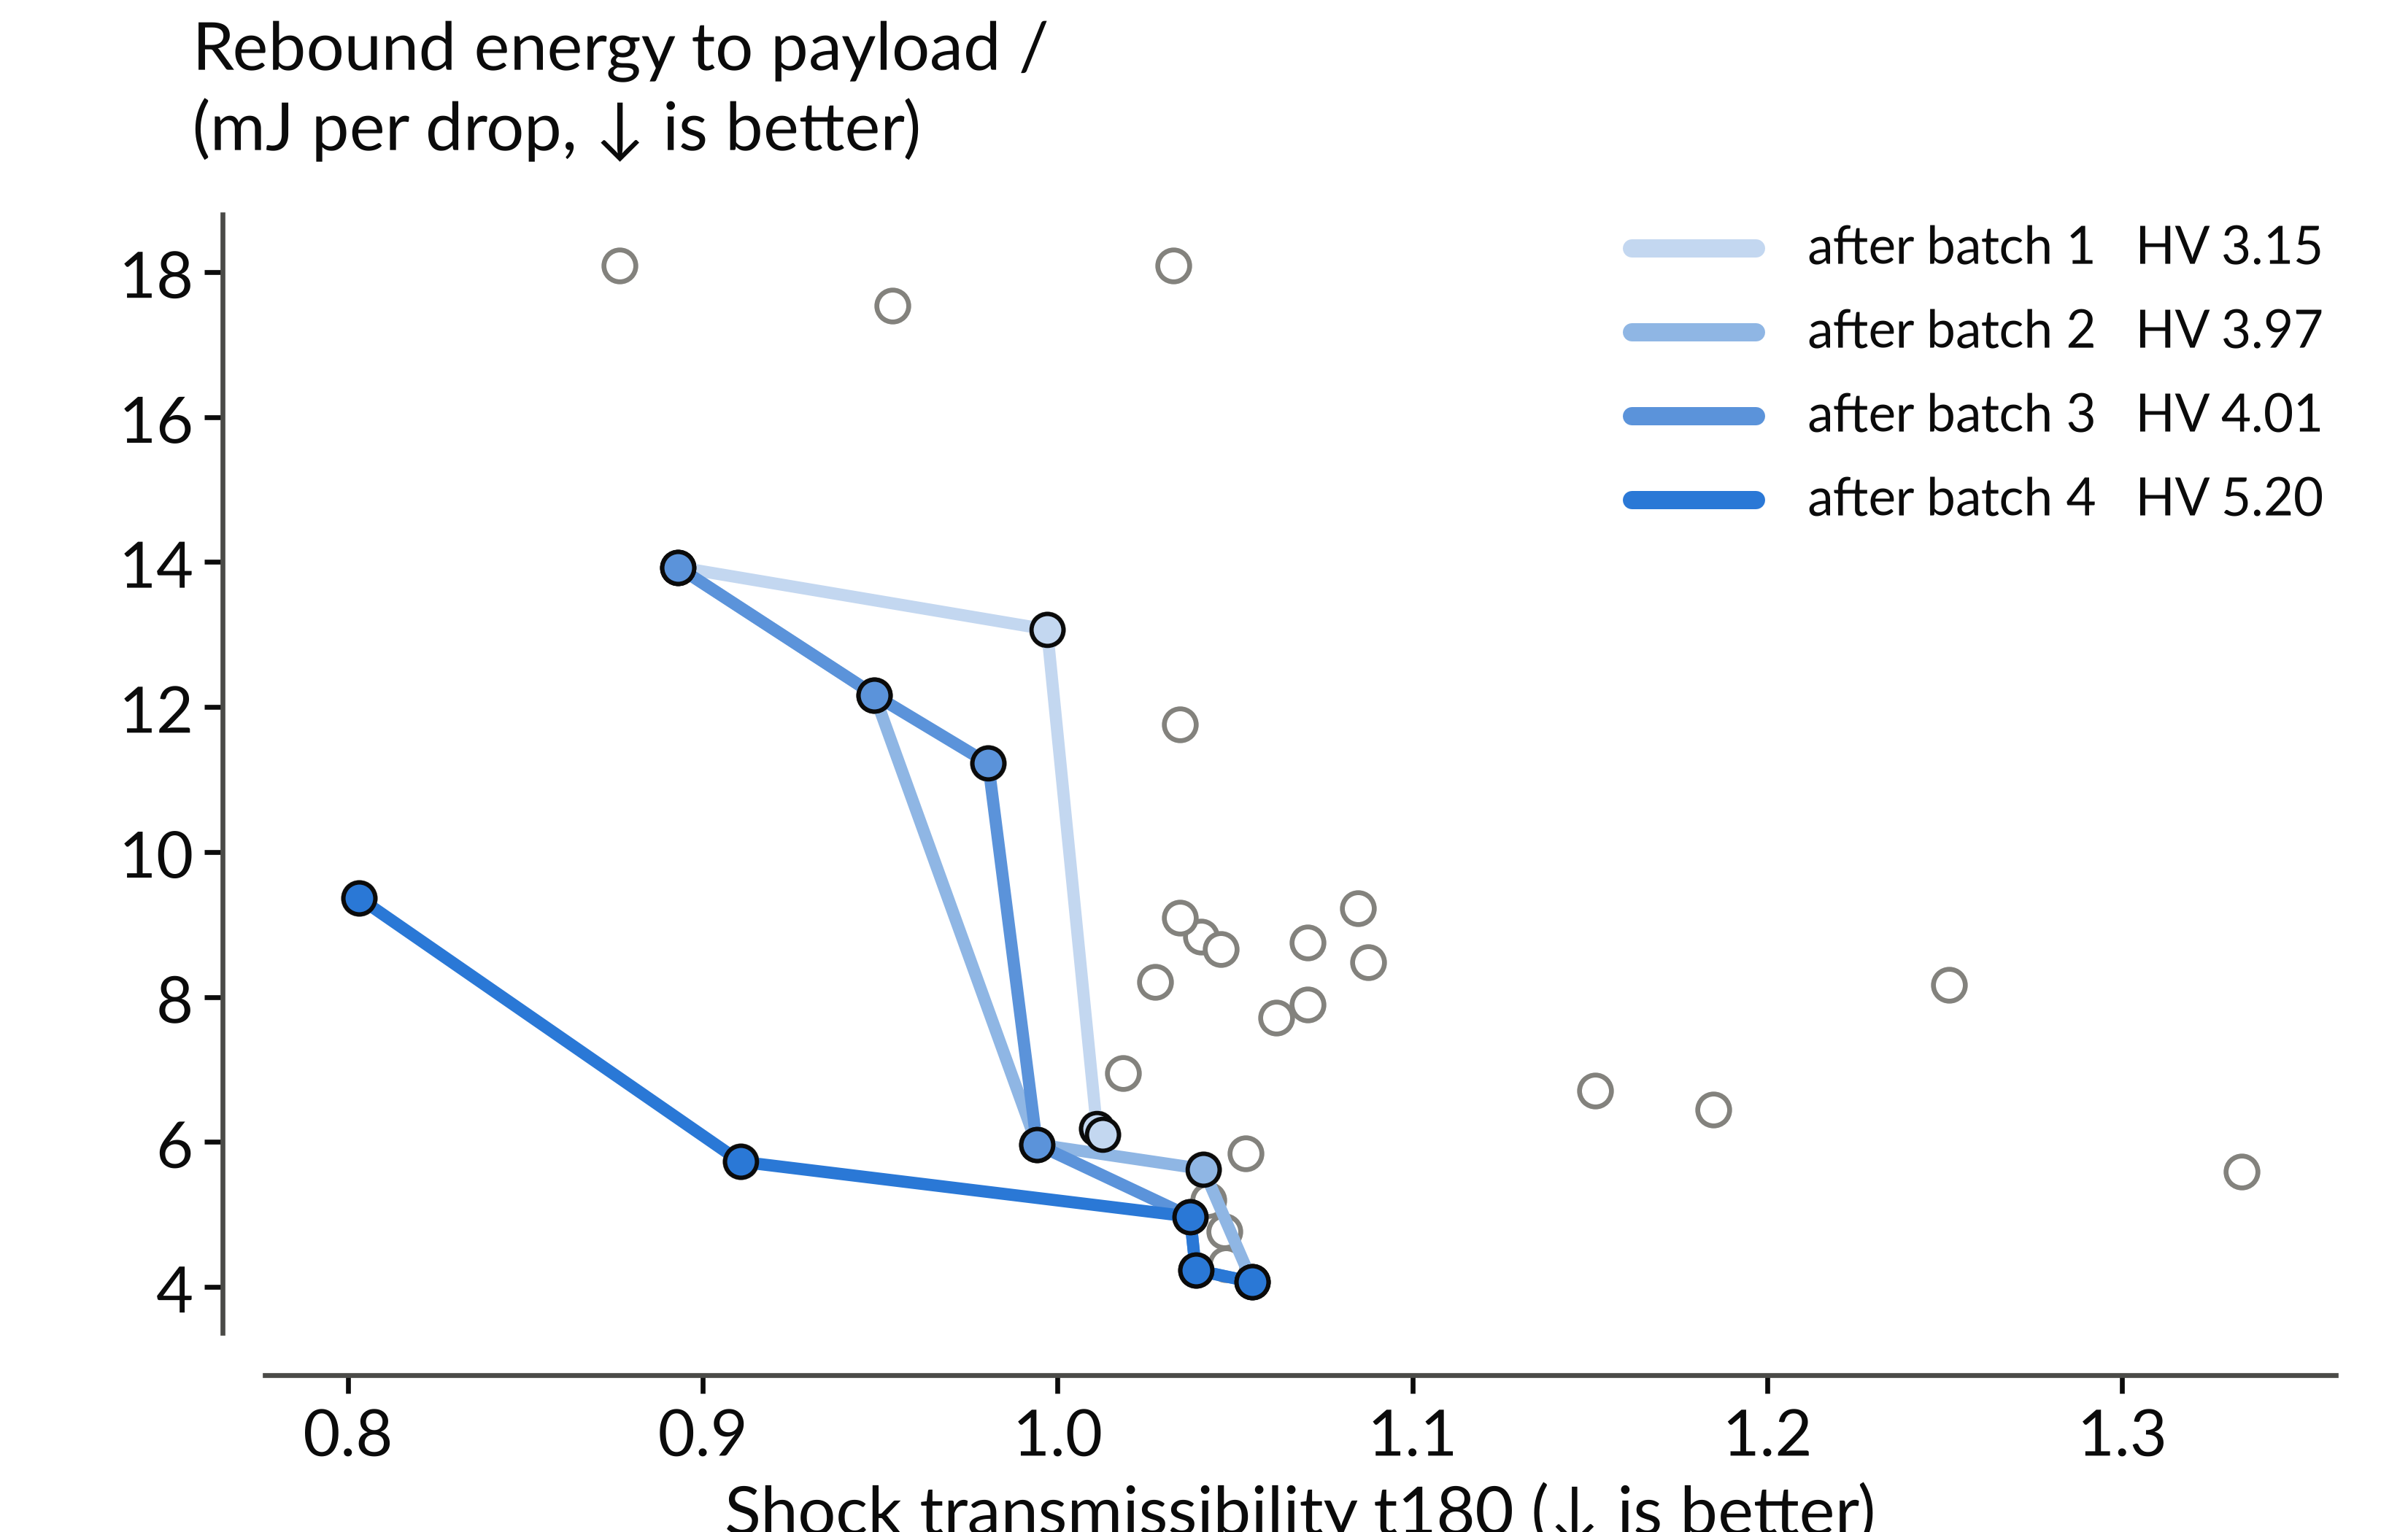
\includegraphics[width=0.85\textwidth]{../figures/bo/t3-prism-bo-front-evolution.png}
  \caption{Measured objective space and front evolution across the
    four batches. Gray circles are all measured articles at their
    stabilized means; the blue lines are the non-dominated fronts
    after each batch, with the dominated hypervolume at the
    $(1.35, \SI{15}{mJ})$ reference in the legend. Batch 2 grew the
    front on the rebound axis, batch 3 filled the knee, and batch 4
    broke the transmissibility floor. Both axes improve downward.}
  \label{fig:front-evolution}
\end{figure*}

\begin{figure*}[t]
  \centering
  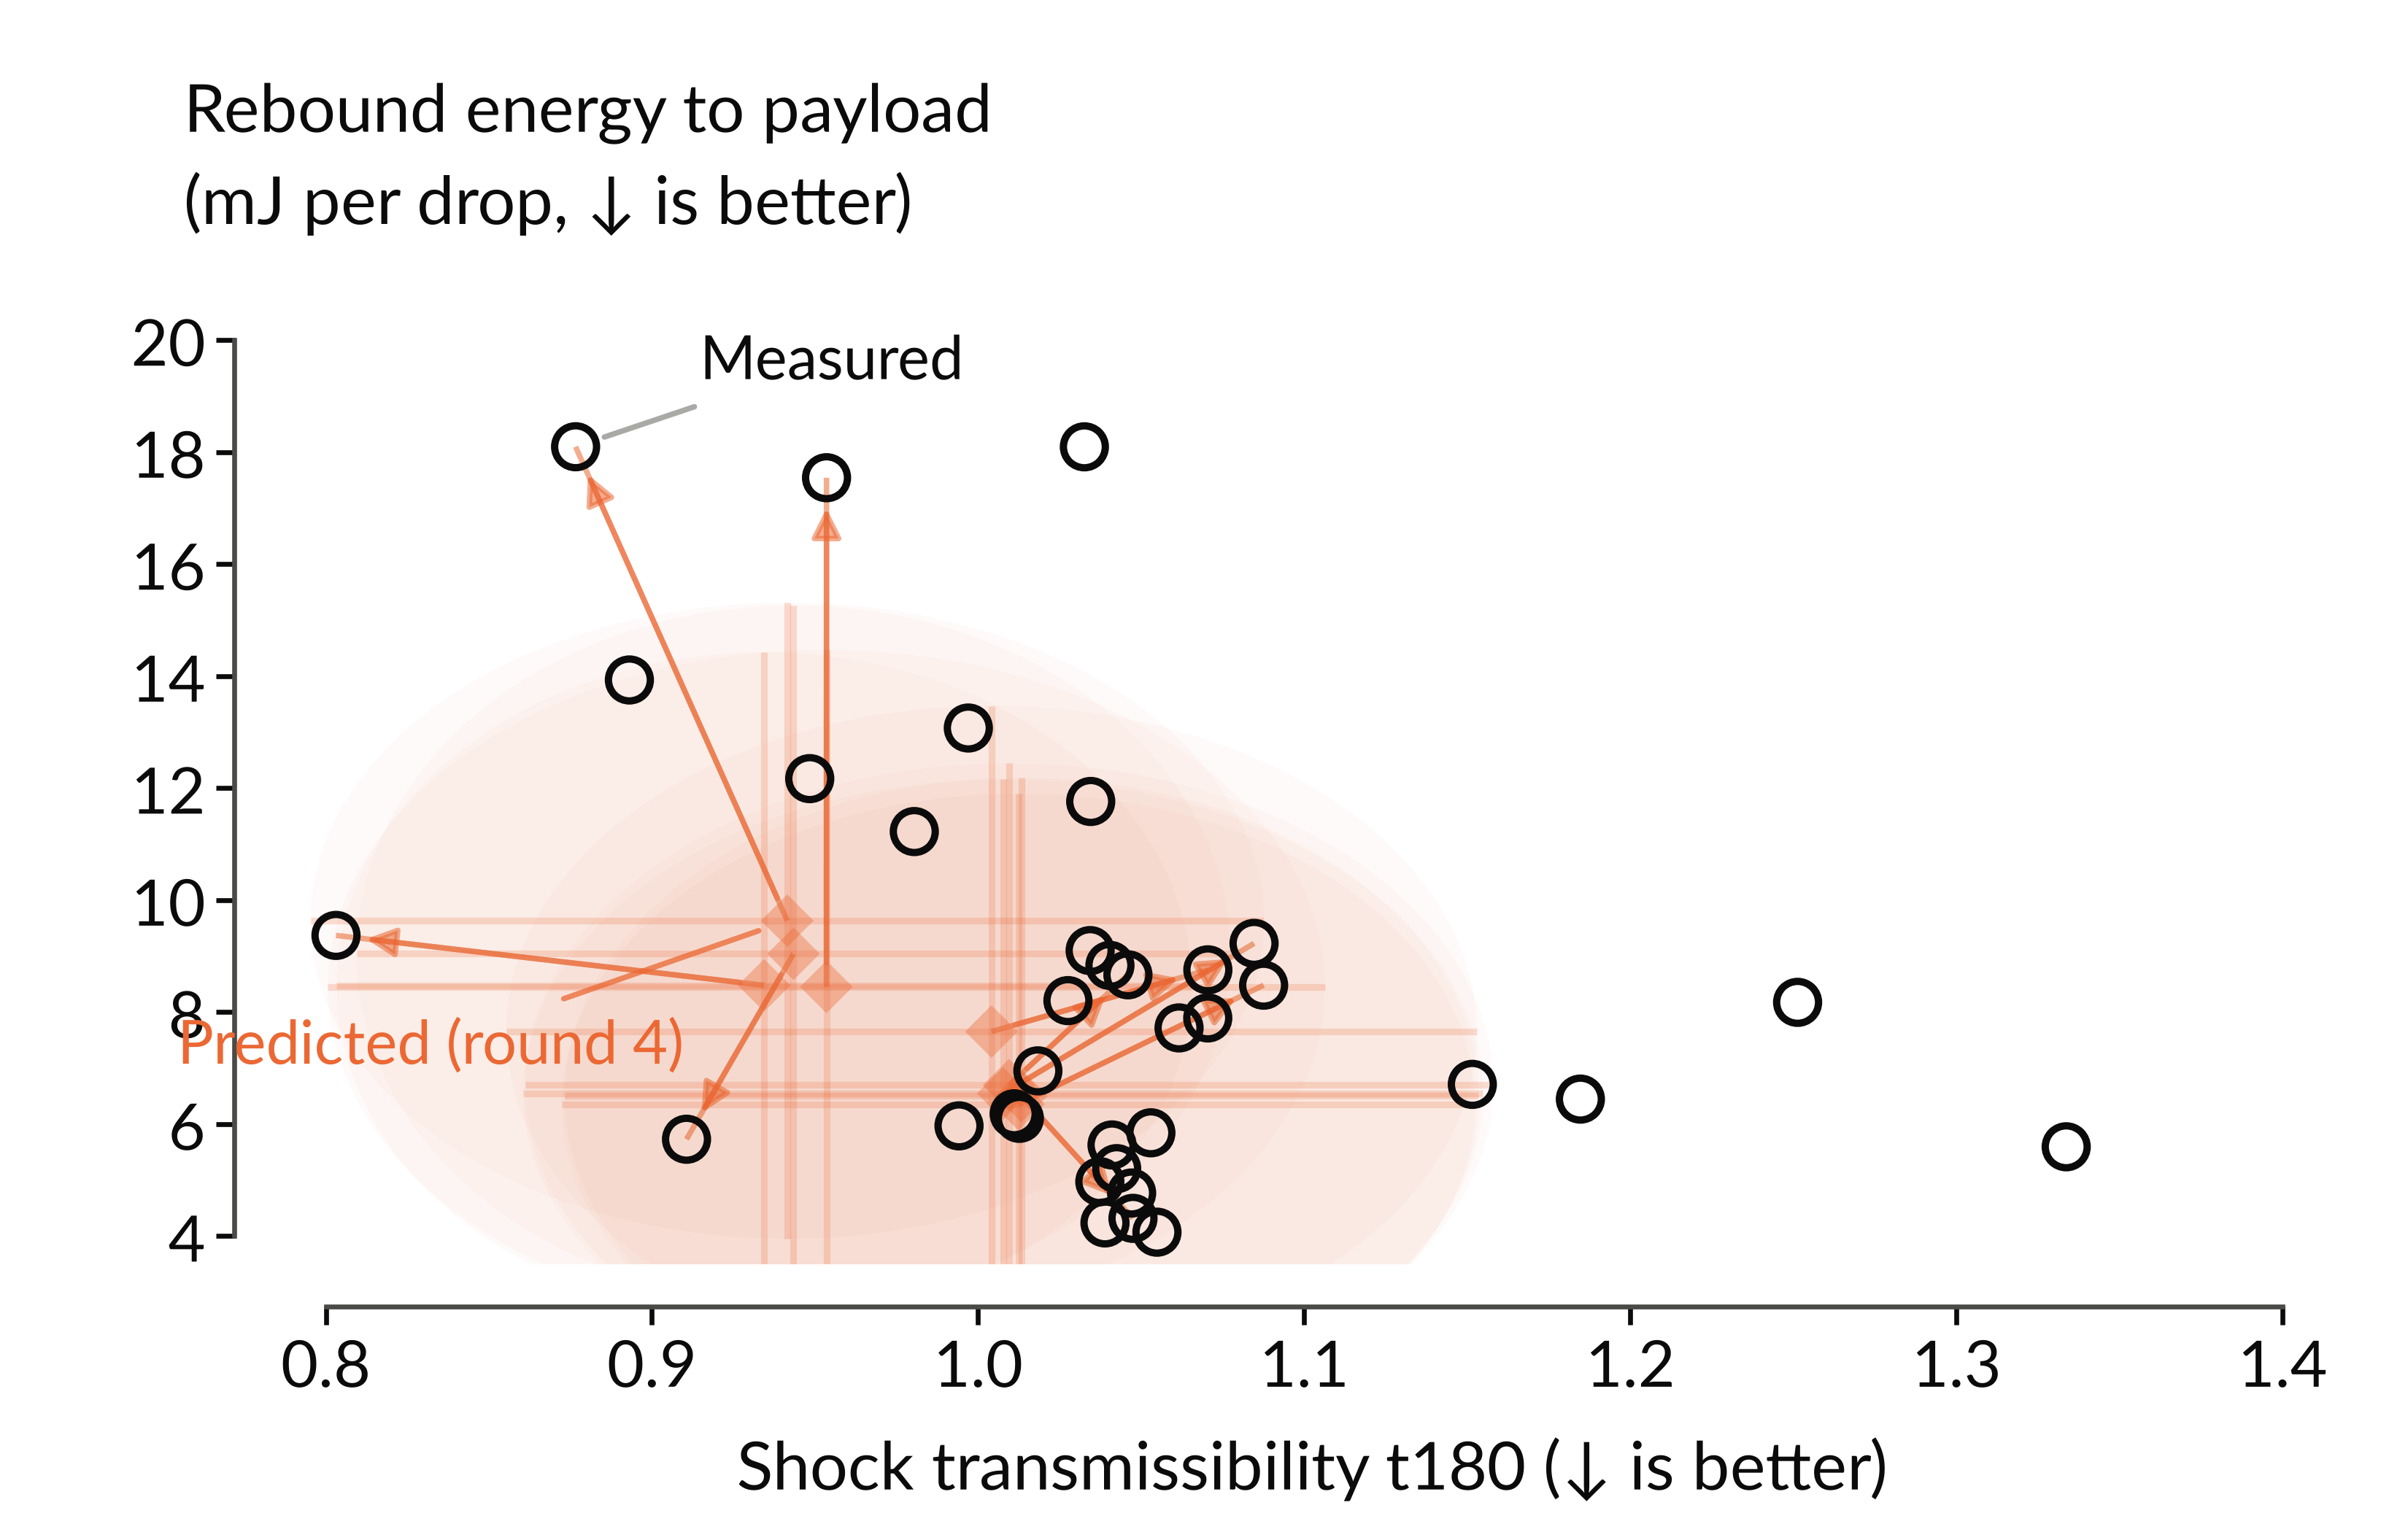
\includegraphics[width=0.85\textwidth]{../figures/bo/t3-prism-bo-round4-predicted-vs-actual.png}
  \caption{Batch-4 predictions against outcomes. Orange diamonds with
    bars are the archived posterior predictions (mean $\pm$ one
    standard deviation) for trials 37 to 45 at recommendation time;
    arrows connect each prediction to its article's measured value
    (black circles; all previously measured articles shown for
    context). The record attenuator corny7 (measured 0.803) is the
    left-most measured point. Both axes improve downward.}
  \label{fig:batch4-pred-vs-meas}
\end{figure*}

\subsection{Surrogate Audits Across the Campaign}
\label{sec:results:audits}

Each refit is audited with leave-one-out cross-validation (LOOCV;
one full NUTS refit per held-out article) and length-scale
diagnostics. Figure~\ref{fig:sensitivity} reports the seed-state
SAASBO feature importances (normalized inverse length scales, median
over the Monte Carlo draws with interquartile whiskers, over the five
design variables plus printed mass). At seven observations for six
correlated inputs these are prior-sensitive model diagnostics only:
no input separates decisively from the equal-share line, and none
supports a claim of variable relevance or ranking.

The honest headline of the cross-validation trajectory is that
held-out point accuracy \emph{declined} as the campaign grew:
$t_{180}$ LOOCV MAPE was 2.9\% with rank correlation $+0.76$ on the
seed state (8 articles, 6 model inputs), 5.4\% and $+0.60$ after
batch 2 (17 articles), and 6.2\% and $+0.19$ after batch 3 (26
articles, 12 inputs); the rebound channel reads 29.3\%, 23.6\%, and
32.2\% MAPE at the same states
(Fig.~\ref{fig:loocv}; the fold-level records are archived with the
campaign data). Three changes landed together and are confounded:
the input space doubled from 6 to 12 while the data grew only from
17 to 26, four of the six added axes carry a single value per batch
and are therefore perfectly confounded with batch, and batch 3
itself added the campaign's largest outliers. The held-out posterior
shrinks predictions toward the pooled mean, so the campaign's
defining extremes are exactly what it misses. The practical stance
this trajectory dictates, and the one the campaign took, is to treat
predicted columns as exploration bookkeeping rather than forecasts:
batch 4's value was the design family it selected and the record it
found, not its point accuracy, and its best-predicted article was
the record. Two further audit facts round out the picture. The
mass-transmissibility correlation fell from $r = 0.82$ over the
seed articles to $0.07$ over the 26 articles of batches 1 to 3, so
the constant-printed-mass projection removed the seed batch's
dominant confound. And the planned head-to-head calibration
comparison against a point-estimated single-task GP with the same
kernel has not yet been run, so no claim is made that SAASBO
outperforms it here.

\begin{figure}[t]
  \centering
  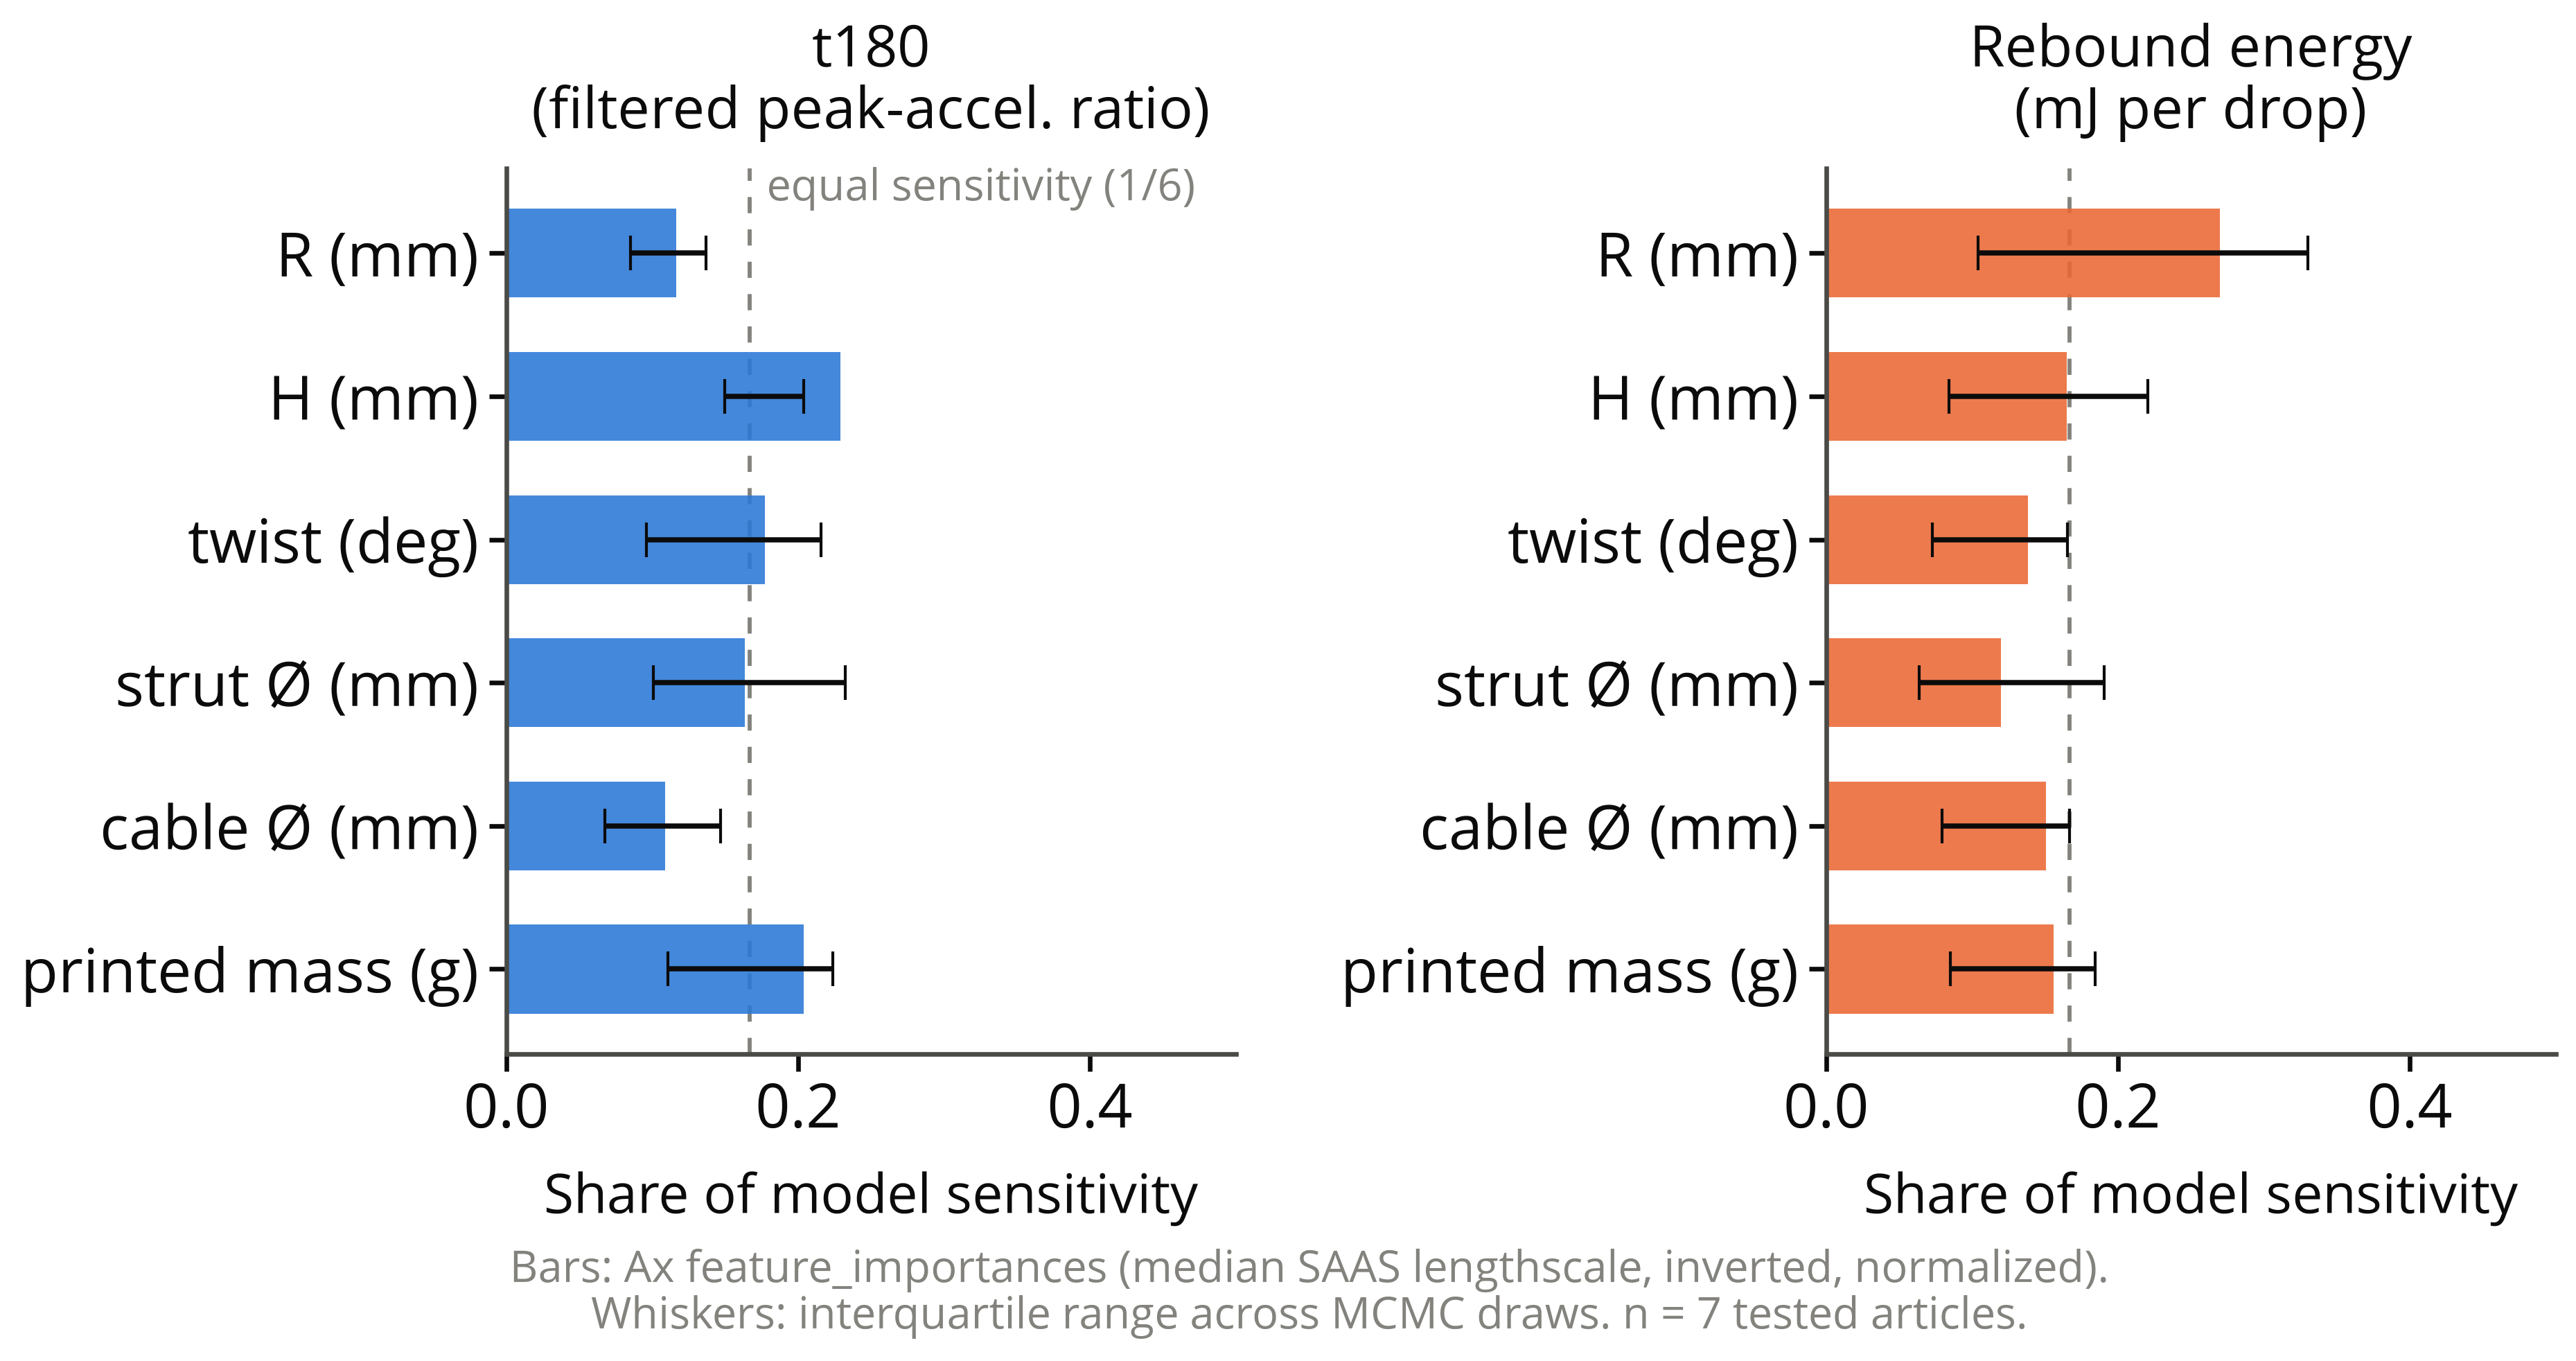
\includegraphics[width=0.92\linewidth]{../figures/bo/t3-prism-bo-round1-feature-importance.png}
  \caption{Seed-state SAASBO length-scale diagnostics per objective
    (normalized inverse length scales; median over MCMC draws,
    interquartile whiskers; inputs are the five design variables plus
    printed mass; the horizontal axis, labeled ``share of model
    sensitivity'' in the plot, is this normalized inverse-length-scale
    diagnostic). No input separates decisively from the equal-share
    line (dashed) at seven mapped articles, and these are
    prior-sensitive model diagnostics, not evidence of variable
    relevance.}
  \label{fig:sensitivity}
\end{figure}

\begin{figure}[t]
  \centering
  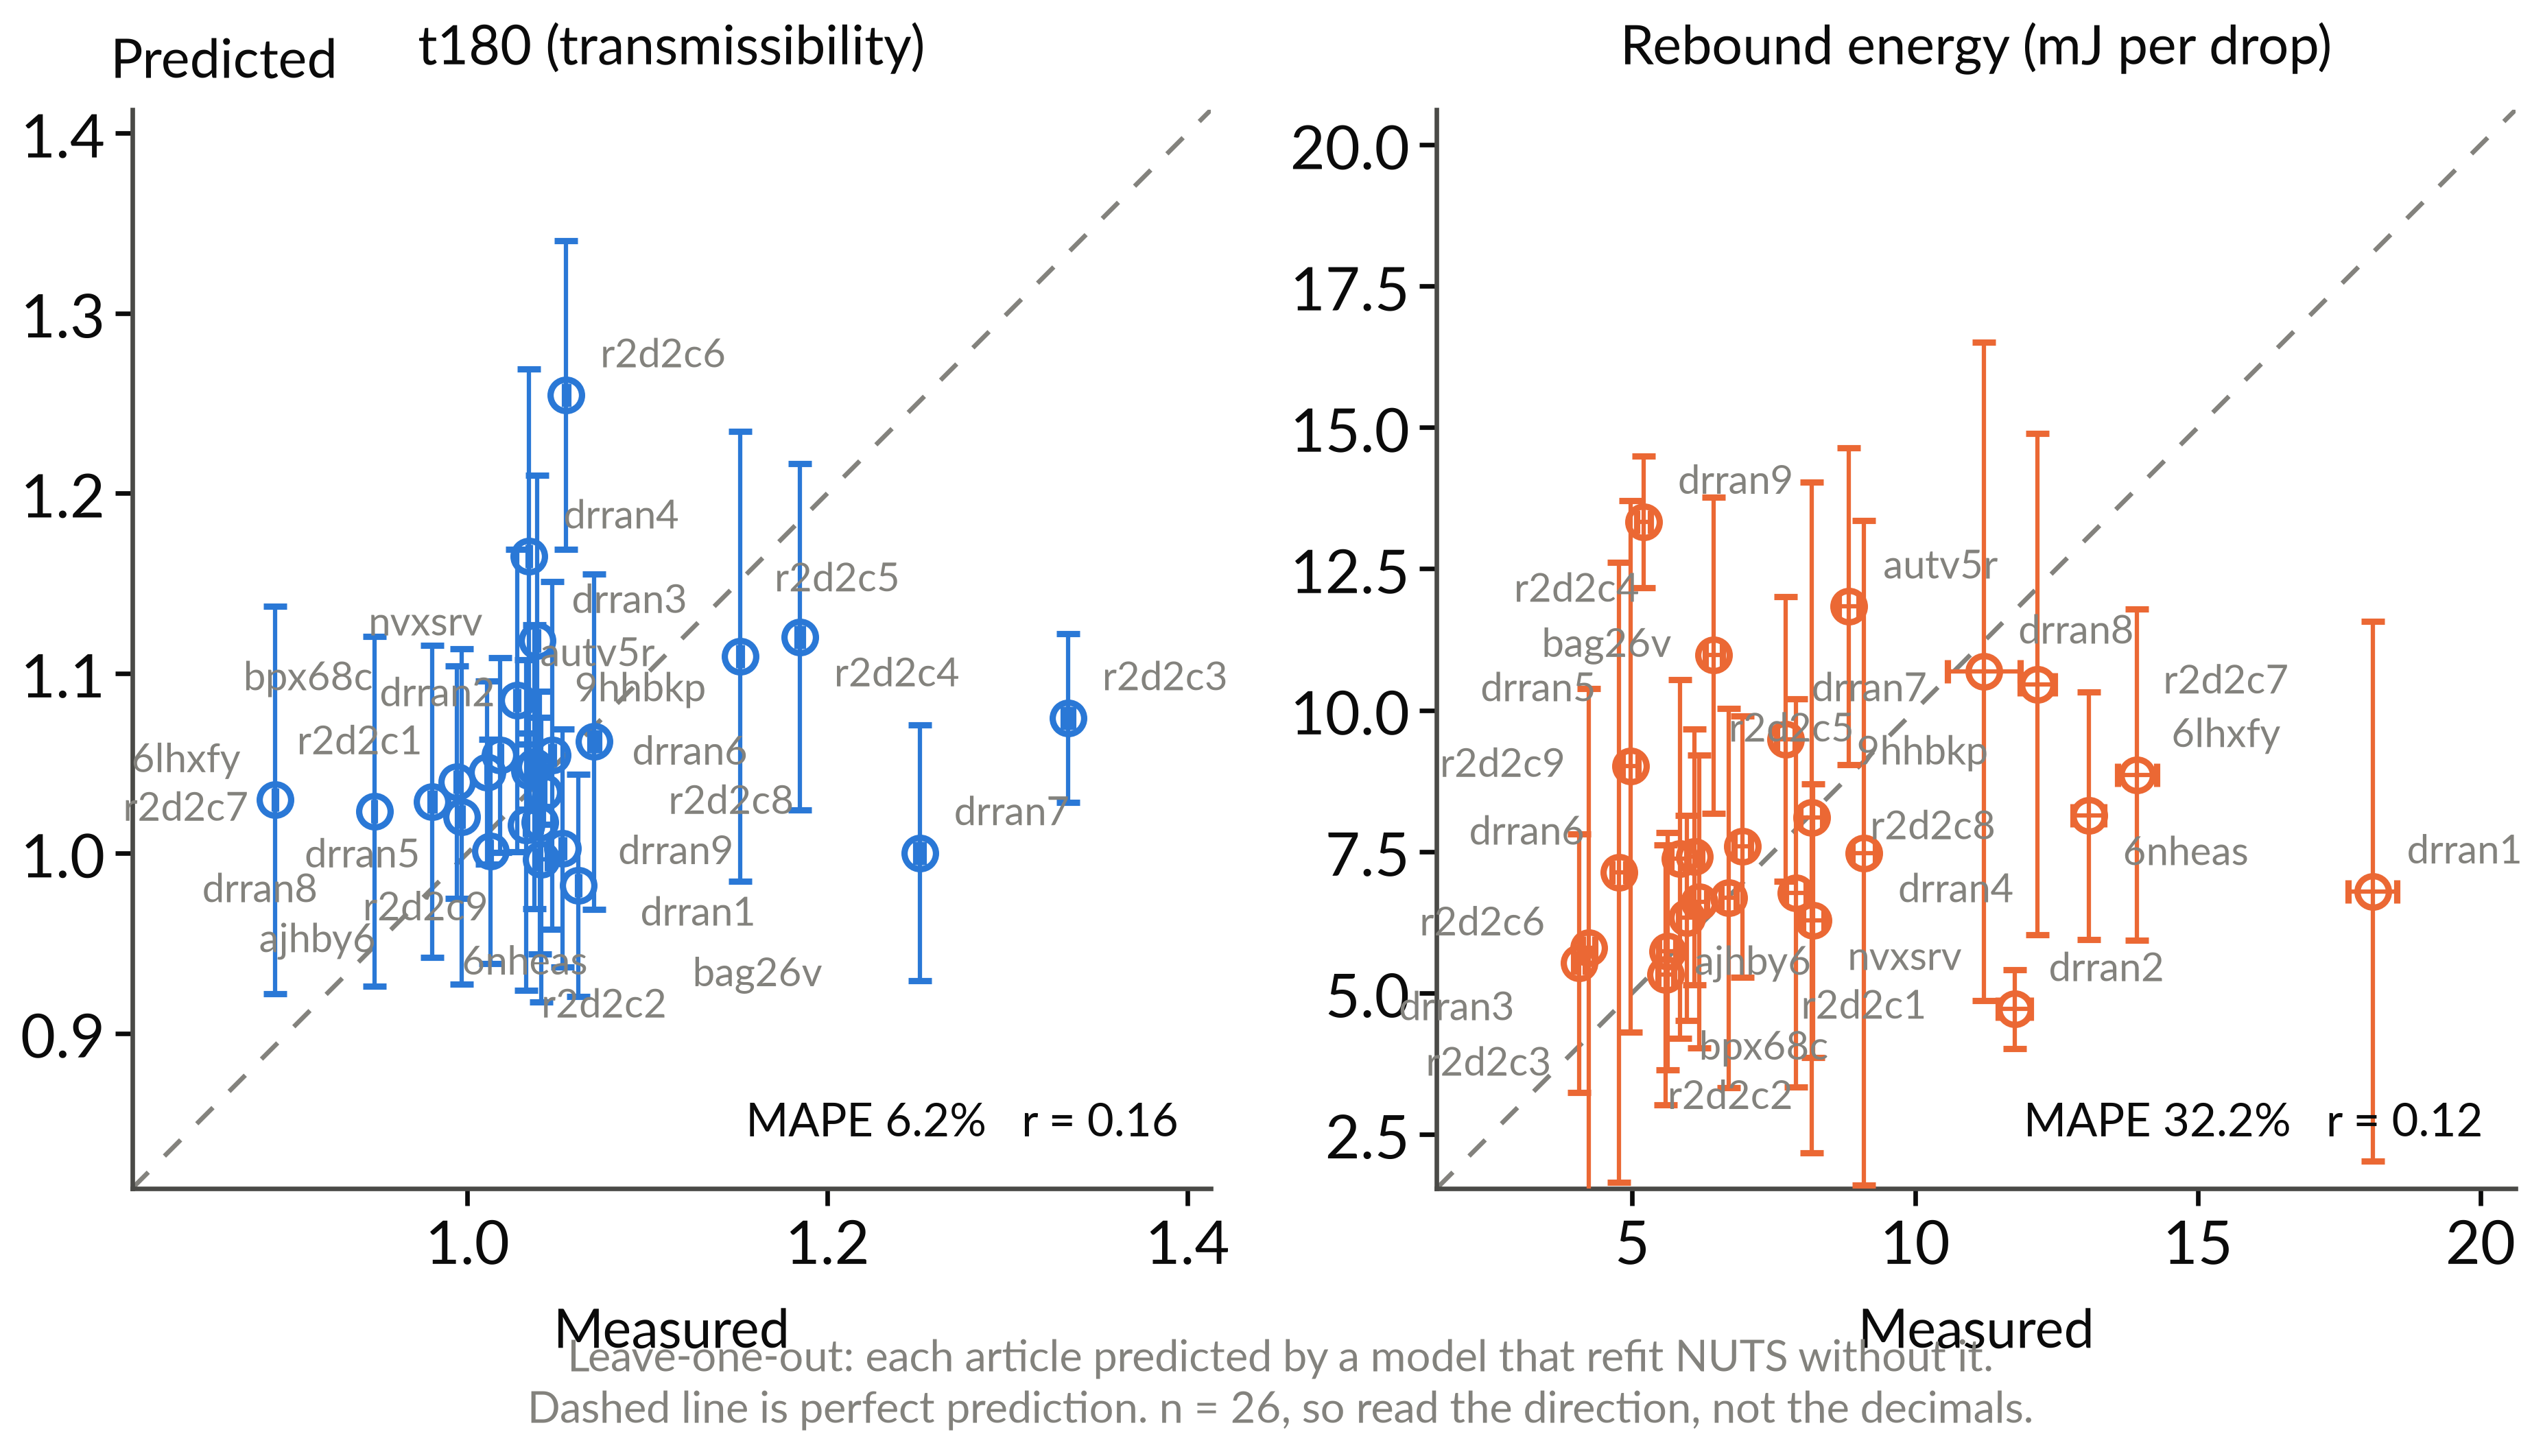
\includegraphics[width=0.92\linewidth]{../figures/bo/t3-prism-bo-round4-loocv.png}
  \caption{Leave-one-out cross-validation of the SAASBO surrogate on
    the 26 articles of batches 1 to 3 (one full NUTS refit per
    held-out article; 12 model inputs). Vertical bars are one
    posterior standard deviation of the held-out prediction;
    horizontal bars are the measured standard error as ingested. The
    dashed line is parity. The held-out posterior shrinks toward the
    pooled mean, so the extremes (r2d2c3, drran7, the seed
    attenuator) are the largest misses.}
  \label{fig:loocv}
\end{figure}

\paragraph{Studies pending} The re-seat confirmations of the batch-4
attenuators (the record article first), any batches beyond the
fourth (a fifth batch is generated and its print files staged, but
nothing from it appears here), the replicate rank-stability study of
Section~\ref{sec:methods:rankstability} (best-, mid-, and
worst-predicted in-sample designs re-printed in nominal triplicate),
the quasi-static crush campaign, and the metal-analog comparison
(Table~\ref{tab:metal-validation}) remain future work; none of their
values appear in this section.


% =============================================================================
\section{Discussion}
\label{sec:discussion}
% =============================================================================

\paragraph{What the campaign establishes} The four measured batches
settle four questions the planned-methods stage could only pose. The
end-to-end loop runs and closes, repeatedly: printed articles,
instrumented characterizations, a fitted fully Bayesian surrogate,
and three successive model-recommended batches whose own
measurements fed the next refit. The measurement distinguishes the
tested articles: the campaign $t_{180}$ means span 0.803 to 1.334,
far beyond within-session drop scatter, though
the batch-3 second pass shows that seating and print variation, not
drop scatter, set the resolution floor for any single article. The
physics is more adversarial than the cushioning intuition suggests:
at this scale and rate, most printed prisms \emph{amplify} the peak
shock reaching their top vertex (26 of 35 articles measured above
unity), which sharpened the campaign question from ``how much does
the architecture cushion'' to ``which corner of the design space
crosses into attenuation, and at what rebound cost.'' And the
batches answered that sharpened question, though not on the first
try: batch 2's forecasts were optimistic on nine of nine articles,
batch 3's best-predicted design was its worst amplifier, and batch 4
then delivered four attenuators from the wide, high-twist,
thin-cable family, led by its best-predicted design at
$t_{180} = 0.803$. The strongest attenuators still tend to carry
large rebound energies (the record article is mid-pack at
\SI{9.4}{mJ}, while the tall batch-4 family shows that near-unity
transmission with low rebound is reachable), so the front remains
genuinely two-dimensional.

\paragraph{Honest accounting of the objective stack} We
pre-registered an adversarial, data-first review of the objective
choices with an external AI referee that was required to commit to
its own objective set from the raw campaign files before reading
ours. Its findings temper the round-1 formulation and set the round-3
revision: the rebound fraction $e_{\mathrm{reb}}$ rests on a ballistic
interpretation of the second contact event that has not yet been
validated against synchronized video (a restrained-versus-unrestrained
check is scheduled); the apparent $t_{180}$-versus-rebound trade-off
is driven substantially by the single strongest attenuator (Spearman
$\rho = -0.39$, $p = 0.38$ across the reliable articles); and
per-drop standard errors are substantially smaller than the
between-article variation, and therefore understate design-level
uncertainty. The campaign's responses were physical rather than
statistical: the batch-3 plate was printed and tested twice, which
measured the same-design shift distribution directly (median
$+1.2\%$, heavy tails; Section~\ref{sec:results:batches}); the
between-seat replication rule now gates every extreme; rebound stays
a candidate constraint pending its ballistic validation; and the
constant-printed-mass projection removed the mass channel the review
flagged. We report this trajectory rather
than presenting the seed-state choices as final because the loop is
the contribution and revising objectives mid-campaign, with the
revision criteria stated in advance, is how such loops behave in
practice.

\paragraph{Mass as a confound and as a design variable} Holding
solid CAD mass constant did not hold printed grams constant: PLA
prints at partial infill while thin TPU cables print near solid, so
the seed articles span \SIrange{18.50}{22.29}{g}, and among the
mapped seed articles mass and $t_{180}$ are correlated
($r = 0.82$). Printed mass is itself induced by the geometry and is
strongly collinear with member dimensions (light articles \emph{are}
the thick-strut, thin-cable corner by construction), so the seed
observations cannot identify separate geometry and mass effects; a
post hoc mass-adjusted regression would be unstable and would
estimate a different, direct-effect quantity. The campaign's answer
was experimental design rather than adjustment: the calibrated
printed-mass model (Supplementary Information) let batches 3 and 4
compare geometries at fixed printed grams (batch mass CVs of 1.7 and
2.3\%), and the mass-transmissibility correlation across the
articles of batches 1 to 3 fell to $r = 0.07$. The confound was
broken by construction, and the mass-aware rebound objective keeps
grams penalized where they physically matter, in the energy returned
to the payload.

\paragraph{Relation to prior art, and why simulation sits outside
the loop} Relative to Pajunen
et~al.~\cite{pajunen2019design}, the present work varies the geometry
under an optimization loop rather than characterizing a single
fabrication condition; relative to Mo
et~al.~\cite{mo2023accelerated}, the loop's ground truth is physical
measurement, and no simulated number enters the objectives, the
acquisition, or candidate priority. That exclusion is a measured
decision, not an omission: an exploratory multi-engine simulation
study conducted alongside the campaign (rigid-body through
finite-element fidelities, archived in the project repository) could
not reproduce the amplification that dominates the measured record
(rigid-strut models cap the transmissibility near unity while most
printed articles exceed it), predicted design-invariant rebound
where the measurement discriminates strongly, and correlated only
weakly with the measured transmissibility. Its constant-mass
fairness constraints and its diagnosis of the seed batch's
mass-rebound confound did shape the campaign design, which is the
screening role we consider simulation to have earned here; anything
more must first demonstrate prospective predictive skill on
articles it has not seen. The measured near-unity
transmission of most seed articles also cautions against reading the
printed-tensegrity literature's attenuation results as generic: the
as-printed cells here are not pretensioned, and activating genuine
pretension in additively manufactured tensegrity (for example through
shrink-on-treatment routes) is an open direction we deliberately
scope out of the present campaign.

\paragraph{Practical considerations and path forward} TPU-PLA
interface durability under repeated impact remains open: no joint
failed during the repeated-drop measurement sessions (more than
1,400 stabilized captures across 35 articles plus the batch-3
second pass), but because
those sessions were not designed as controlled fatigue tests, the
observation does not establish interface durability, and pull-out
and fatigue characterization of the internal-anchor joint is an area
of planned follow-on work. Sensitivity to
print-process covariates (the print key logs defects, humidity, and
the mid-batch nozzle change for exactly this purpose) and transfer to
other material pairs likewise remain open. In the future we plan
the re-seat confirmations of the batch-4 attenuators, the replicate
rank-stability study of Section~\ref{sec:methods:rankstability}, the
metal-analog rank-transfer comparison of
Section~\ref{sec:methods:validation}, quasi-static testing as an
extension of the characterization
(Section~\ref{sec:methods:testing}), pretension activation, tiled
multi-cell absorbers and lattices~\citep{sabounizawadzka2024experimental},
and miniaturization to crutch-tip envelopes: long-term crutch use is
associated with substantial upper-extremity overuse injury and
ground-reaction-force impulses~\citep{requejo2005upperextremitykinetics,
rasouli2020walkingassistanceusing, manocha2021injuriesassociatedwith,
brasilbarrosdasilva2022painmappingand,
dozono2015peripheralneuropathiesin}; existing
spring-loaded~\citep{segura2007mechanicsofambulation,
zhang2011biomechanicalevaluationof} and
polymer-damped~\citep{macgillivray2016theinfluenceof} tip designs
reduce loading rate but not peak transmitted force, and recent
tensegrity crutch concepts~\citep{gu2026tensegritycrutches} and
open-source 3D-printed crutch
work~\citep{mottaghi2025opensource3dprintable} suggest a plausible
translation path, with adjacent footwear and orthotic lattice
studies~\citep{wang2025porouslatticestructure,
zhang2024pressurereducingdesignof,
janarthanan2024additivemanufacturingof} providing transferable design
heuristics.

\paragraph{Limitations} The measured evidence base is 35 articles
across four batches, but with one mechanical-response article per
design in the fit: only batch 3 has a second printed-and-tested set,
and that replication is what exposed the seating and print
sensitivity, so every single-article extreme, including the batch-4
record, is provisional until its re-seat. The drop protocol probes
one height, one impact surface, and axial loading only; the
specimens never leave the elastic regime, so crush-energy metrics
await the quasi-static campaign; per-specimen energy absorption in
joules is not recoverable from the current rig (the falling-mass and
displacement channels required for a force integral are not
instrumented); the four filament axes carry one value per batch and
are unidentified; the held-out prediction skill of the surrogate
declined as the input space grew
(Section~\ref{sec:results:audits}); one tested seed article lacks a
design mapping, one seed design's official article assignment
carries a recorded discrepancy, and two seed designs have no session
record; and all results are from a single printer, material pair,
and cell topology. The replication rule, the planned re-seat
confirmations, the replicate rank-stability study
(Section~\ref{sec:methods:rankstability}), and the metal-analog
protocol (Section~\ref{sec:methods:validation}) are the designed
responses to these limits.

% =============================================================================
\section{Conclusions}
\label{sec:conclusions}
% =============================================================================

We have presented an experiment-driven Bayesian-optimization
framework for designing multi-material 3D-printed tensegrity-inspired
energy absorbers, with TPU used in place of the traditional tension
elements and PLA members carrying compression most of the time, and
we have run it through the recommend, fabricate, measure, and update
cycle three times on physical hardware. The framework parameterizes a
$T_3$-prism family (five geometry variables, joined in batch 3 by
infill and filament process variables) under a constant-mass fairness
projection, fabricates each candidate in a single multi-material FDM
build with TPU tendons anchored inside the PLA strut ends,
characterizes every article with repeated instrumented drops (101
stabilized captures in the seed batch, about twenty thereafter), and
updates a fully Bayesian Gaussian-process
surrogate~\citep{balandat2020botorch, eriksson2021saasbo} that
recommends the next batch. Across the four measured batches (35
articles), the transmissibility spanned 0.803 to 1.334, most
articles amplified the peak shock, and the model-recommended batches
grew the dominated hypervolume 65\% over the Sobol seed front,
ending with a front whose five members are all model-chosen; the
batch-4 best-predicted design set the program record at
$t_{180} = 0.803$, ten percent below the best seed article, and
awaits its re-seat confirmation under the campaign's replication
rule. A second print-and-test pass of one batch showed that seating
and print variation, not drop-to-drop scatter, bound design-level
claims, which is the workflow lesson we consider most transferable.
The workflow is a candidate for other experimentally
evaluated architected structures whose constitutive response is
difficult to calibrate from first principles, but transfer beyond this
printer, material pair, topology, and axial impact condition remains
untested.

% =============================================================================
% Back matter
% =============================================================================
\section*{Acknowledgment} % ASME requests this exact spelling, singular.

This work was supported by the Brigham Young University Mentored
Research Grant program. The authors thank the undergraduate researchers
who carried out the multi-material printing and impact testing, and the
graduate co-mentor who supported day-to-day operations.
\todo{Confirm exact grant numbers and acknowledge any
NASA/Utah-Space-Grant-Consortium support per
acknowledgment-text guidelines.}

\section*{Funding Data}
\begin{itemize}
  \item Brigham Young University Mentored Research Grant.
\end{itemize}
\todo[inline]{Insert the MRG award number, and add the Utah NASA Space
Grant Consortium award if applicable.}

\section*{Conflict of Interest}
The authors declare no conflict of interest.

% Print the list of pending TODOs at the end -- the [disable] option
% on todonotes hides this automatically in the clean wrapper.
\listoftodos[Pending TODOs and figure/table placeholders]

% -----------------------------------------------------------------------------
% References (ASME numeric style; uses asmejour.bst)
% -----------------------------------------------------------------------------
\bibliographystyle{asmejour}
\bibliography{references}

\end{document}
:
%   \def\TODOOPTS{disable}    % manuscript.tex
%   \def\TODOOPTS{}           % manuscript-todos.tex
% =============================================================================

% PDF/A metadata (added in 2022; required by current asmejour for accessibility)
\DocumentMetadata{%
  lang        = en-US,
  pdfstandard = A-3u,
  pdfversion  = 1.7,
}

% Class options (see asmejour-template.pdf for the full list):
%   * lineno       -- numbered lines for review markup (run pdflatex twice)
%   * singlecolumn -- one-column draft layout (drop for ASME two-column final)
%   * nocopyright  -- suppress ASME copyright footer until acceptance
%   * upint, varvw -- typographic preferences carried over from the template
%   * hyphenate    -- allow hyphenation in typewriter font
\documentclass[lineno,nocopyright,upint,varvw,hyphenate]{asmejour}

\allowdisplaybreaks % from amsmath; multiline equations may break across pages

% --- Additional packages ---
% asmejour already loads: graphicx, hyperref, natbib, amsmath, amssymb,
% xcolor, booktabs, subcaption, caption, lineno, etc. Avoid re-loading those.
\usepackage{siunitx}
% House style: no en dashes anywhere, including ranges; siunitx ranges
% therefore render as "X to Y" rather than "X--Y".
\sisetup{range-phrase = { to }, range-units = single}
% tikz for measurement callouts overlaid on the printed-prototype photograph
% (Fig.~\ref{fig:printed-prototypes}); asmejour already loads graphicx/xcolor.
\usepackage{tikz}
\usetikzlibrary{arrows.meta}
% todonotes for in-margin TODO/figure-placeholder markers; toggled by the
% wrapper file (\TODOOPTS = "disable" hides everything; "" shows all).
\usepackage[\TODOOPTS,colorinlistoftodos,textsize=footnotesize]{todonotes}
\setlength{\marginparwidth}{2cm}

% Convenience macros that vanish along with todonotes when [disable] is set.
\newcommand{\figplaceholder}[3][]{%
  % #1 = optional [width]; #2 = label; #3 = caption / what to draw
  \begin{figure}[ht]
    \centering
    \fbox{\parbox[c][3.2cm][c]{0.85\linewidth}{\centering\textit{Figure
        placeholder: #3}}}%
    \caption{\textit{Placeholder.} #3}
    \label{fig:#2}
  \end{figure}%
  \todo[inline,color=orange!30]{Figure \texttt{#2}: #3}%
}

% Synthetic-placeholder (dummy) data convention. Any value that is a
% stand-in rather than a measurement is typeset in this violet color in
% BOTH wrappers (clean and todos) so no reader can mistake it for data.
% As of 2026-09-15 the Results carry no violet values: the former dummy
% round-2 numbers were replaced by the measured batch 2-4 record
% (manuscript/data/, snapshotted from the campaign branch at e25ebf5).
% The macro stays defined for future placeholders.
\definecolor{dummydata}{RGB}{142,68,173}
\newcommand{\dummy}[1]{\textcolor{dummydata}{#1}}

\newcommand{\tabplaceholder}[2]{%
  % #1 = label; #2 = caption / contents description
  \begin{table}[ht]
    \centering
    \caption{\textit{Placeholder.} #2}
    \label{tab:#1}
    \begin{tabular}{@{}lll@{}}
      \toprule
      Column A & Column B & Column C \\
      \midrule
      \multicolumn{3}{c}{\textit{(table contents pending)}} \\
      \bottomrule
    \end{tabular}
  \end{table}%
  \todo[inline,color=orange!30]{Table \texttt{#1}: #2}%
}

% --- PDF metadata ---
\hypersetup{%
  pdfauthor   = {Jeffrey R. Hill and Sterling G. Baird},
  pdftitle    = {Experiment-Driven Bayesian Optimization of the Impact Response
                 of Multi-Material 3D-Printed Tensegrity-Inspired Structures},
  pdfkeywords = {tensegrity, multi-material 3D printing, Bayesian optimization,
                 impact mitigation, design of experiments},
  pdfsubject  = {Manuscript draft for ASME Journal of Mechanical Design},
}

% --- Journal name (printed in the running head; omit "Journal of") ---
\JourName{Mechanical Design}

\begin{document}

% =============================================================================
% Author block(s) -- one \SetAuthorBlock per author (or per shared affiliation)
% Mark corresponding author(s) with \CorrespondingAuthor (no space before).
% =============================================================================
% Author order per @me-madsen review (PR #20): equal-contribution and
% corresponding-author scheme is \textsuperscript{*} = equal contribution,
% \textsuperscript{\dag} = also equal contribution, \textsuperscript{\ddag} =
% corresponding author (see legend \todo after \maketitle).
\SetAuthorBlock{Marcus E. Madsen\textsuperscript{*}}{%
  Department of Mechanical Engineering,\\
  Brigham Young University,\\
  Provo, UT 84602, USA
}

\SetAuthorBlock{Audrey K. Christiansen\textsuperscript{*}}{%
  Department of Mechanical Engineering,\\
  Brigham Young University,\\
  Provo, UT 84602, USA
}

\SetAuthorBlock{Jinkwan Han\textsuperscript{*}}{%
  Department of Mechanical Engineering,\\
  Brigham Young University,\\
  Provo, UT 84602, USA
}

\SetAuthorBlock{Jeffrey R. Hill\textsuperscript{\dag\ddag}\CorrespondingAuthor}{%
  Department of Mechanical Engineering,\\
  Brigham Young University,\\
  Provo, UT 84602, USA\\
  email: jeff.hill@byu.edu
}

\SetAuthorBlock{Sterling G. Baird\textsuperscript{\dag\ddag}\CorrespondingAuthor}{%
  Department of Mechanical Engineering,\\
  Brigham Young University,\\
  Provo, UT 84602, USA\\
  email: sterling.baird@byu.edu
}

\title{Experiment-Driven Bayesian Optimization of the Impact Response of
       Multi-Material 3D-Printed Tensegrity-Inspired Structures}

% Keywords are printed at the end of the abstract; must precede \end{abstract}.
\keywords{tensegrity, multi-material 3D printing, Bayesian optimization,
          impact mitigation, design of experiments}

% -----------------------------------------------------------------------------
% Abstract -- JMD requires 150--200 words, Latin characters only (no math),
% structured as background, approach, results, conclusions.
% -----------------------------------------------------------------------------
\begin{abstract}
Tensegrity-inspired rigid-soft architectures are candidates for impact
mitigation, but their transmitted-shock response is difficult to predict
from simulation alone. We report an experiment-driven Bayesian
optimization campaign over a co-printed polylactic-acid/thermoplastic-%
polyurethane three-strut prism family. The search space begins with five
continuous geometry variables and, from the third batch, adds
per-article infill densities and batch-level filament settings.
Candidate geometries are projected to a common mass budget and
fabricated in single multi-material builds, and each article is
characterized by repeated instrumented drops: 101 stabilized captures in
the seed batch and about twenty thereafter. The optimizer jointly
minimizes the filtered peak-acceleration ratio (transmissibility) and
the rebound energy returned to the payload. Most printed articles
amplify the peak shock, so the campaign question became which corner of
the design space attenuates. Across one Sobol seed batch and three
model-recommended batches, 35 articles in all, the dominated hypervolume
grew 65 percent, the final Pareto front is entirely model-chosen, and
the fourth batch's best-predicted design set the program record,
lowering transmissibility to 0.803, ten percent below the best seed
article. A second print-and-test pass of one batch showed that seating
and print variation, not drop-to-drop scatter, limit design-level
claims, motivating the replication rule we adopt.
\end{abstract}

\maketitle

\begin{center}
  \fcolorbox{dummydata}{dummydata!6}{\parbox{0.94\linewidth}{\small
  \textcolor{dummydata}{\textbf{Draft note (remove before submission):} this
  draft is written at the intended final scope of the study, and any value
  printed in this violet color is a synthetic placeholder rather than a
  measurement. As of 2026-09-15 the Results contain no violet values: all
  four reported batches (35 articles) are measured data from the committed
  campaign record. Still pending, and written as future work rather than
  as results: the re-seat confirmation of the batch-4 record article, any
  batches beyond the fourth, the replicate rank-stability study (best-,
  mid-, and worst-predicted in-sample designs in nominal triplicate), the
  quasi-static crush campaign, the metal-analog comparison, and the
  archival (Zenodo) code release.}}}
\end{center}

\todo[inline]{\textbf{Author order / contributions (per @me-madsen).} Planned
  order: Marcus E. Madsen\textsuperscript{*}, Audrey K.
  Christiansen\textsuperscript{*}, Jinkwan Han\textsuperscript{*}, Jeffrey R.
  Hill\textsuperscript{\dag\ddag}, Sterling G. Baird\textsuperscript{\dag\ddag},
  where \textsuperscript{*}~=~equal contribution, \textsuperscript{\dag}~=~also
  equal contribution, and \textsuperscript{\ddag}~=~corresponding author.
  Confirm affiliations and add emails for M.~Madsen, A.~Christiansen, and
  J.~Han, and typeset the equal-contribution footnote per ASME JMD style.}

% =============================================================================
% Body -- IMRaD structure per JMD submission instructions
% =============================================================================
\section{Introduction}
\label{sec:introduction}

Tensegrity structures are assemblies of rigid compression members
suspended within a continuous network of tension members; their defining
property, that no two rigid bars touch, yields lightweight assemblies with
remarkable strength-to-weight ratios and tunable nonlinear mechanical
responses~\citep{skelton2009tensegrity, sultan2009tensegrity}. These
properties have made tensegrity attractive across scales, from
metamaterial unit cells~\citep{amendola2014experimental,
zhang2018tensegrity, fraternali2015tensegrity} to compliant impact-absorbing
robots developed for planetary landing~\citep{agogino2018superball,
caluwaerts2014superball, sabelhaus2015system, vespignani2018design,
deitrich2022titan}. Recent work has shown that \emph{tensegrity-inspired}
unit cells can be directly 3D-printed and exhibit load-limiting plateaus
under drop-weight impact~\citep{pajunen2019design}, opening a path
toward additively manufactured architected absorbers. Throughout, we use
\emph{tensegrity-inspired} for printable cells that borrow the separated
compression-member and tension-network geometry of tensegrity while
relaxing defining mechanical conditions of classical tensegrity. In the
present specimens, the TPU tension elements are extensible, the PLA struts
may share printed junctions, and no pretension is activated or measured.
We therefore do not claim classical tensegrity, prestress-stabilized
behavior, or equivalence to an ideal cable-strut prism.

Multi-material fused-deposition modeling (FDM) that pairs a rigid polymer
such as polylactic acid (PLA) with a soft, rate-dependent elastomer such as
thermoplastic polyurethane (TPU) has been used to fabricate rigid-soft
architected energy absorbers on a single platform: thick-panel
origami metamaterials with PLA panels and TPU hinges~\citep{ye2023multimaterial}
and ABS/TPU honeycombs with tunable stiff/flexible
proportions~\citep{khatri2024energy}. The same rigid-soft co-printing
capability makes it possible to rapidly fabricate diverse tensegrity-inspired
geometries, which adopt a discrete-compression/continuous-tension topology
rather than an origami or honeycomb one. Although extruded TPU does not behave
as an idealized
inextensible cable, its rate-dependent damping is a desirable property
for impact-absorption applications and complements the elastic stiffness
of the PLA compression members rather than competing with it.

Designing such architected absorbers is fundamentally a
\emph{design-of-experiments} problem: the configuration space spanned by
strut geometry, tension-element cross-section, connectivity, and
unit-cell tiling is large; each candidate must be physically printed
and tested; and the relevant impact-performance metrics (the shock
transmitted across the structure and the energy returned to the
protected payload) are noisy and partially correlated. Bayesian
optimization (BO) is well-matched to this regime, having driven
breakthroughs from hyperparameter tuning of
AlphaGo~\citep{chen2018bayesianoptimizationalphago} to sustainable
concrete~\citep{ament2023sustainable}, autonomous discovery of organic
laser emitters~\citep{striethkalthoff2024delocalized}, and architected
materials~\citep{mo2023accelerated, zhang2021bo}.
The gap this paper addresses is the combination of these two ideas:
Pajunen et~al.~\cite{pajunen2019design} printed tensegrity-inspired
cells under a single fabrication condition with no optimization loop,
and Mo et~al.~\cite{mo2023accelerated} closed a multifidelity BO loop
entirely in simulation. Among the studies reviewed here, prior work
separately demonstrates physical impact testing of printed
tensegrity-inspired structures, rigid-flexible additive fabrication,
and Bayesian optimization of architected materials; we found no prior
report combining these elements in a BO campaign over co-printed
multi-material tensegrity-inspired hardware with physical impact
measurements as the optimization ground truth. The campaign reported
here closes the recommend, fabricate, measure, and update cycle three
times over: a Sobol seed batch trains the surrogate, and each of three
successive model-recommended batches was fabricated, tested under the
identical protocol, and folded back into the refit that produced the
next.

We emphasize one framing point at the outset: the printed PLA/TPU
$T_3$ prism studied here is a testbed for developing and validating
the closed-loop workflow, not flight hardware, and not the end of the
design space we intend to search. The planetary-lander setting
motivates the objectives (limit the shock delivered to a payload,
limit the energy returned to it) and the constant-mass fairness
constraint, but the contribution is the loop itself: a stepping stone
toward optimizing tensegrity-inspired structures generally, agnostic
to the eventual application scale.

\paragraph{Contributions} This paper makes the following contributions:
\begin{enumerate}
  \item A parameterized family of multi-material 3D-printable
    tensegrity-inspired unit cells that uses TPU in place of the
    tension elements of the traditional tensegrity topology, with PLA
    members that carry compression most of the time (the cells are
    not prestressed, so neither member type acts as a pure tension or
    compression element; under impact some tendons stretch while
    others buckle). The TPU tendons are anchored \emph{inside} the
    ends of each PLA strut, the strut acting as a rigid cage in which
    the cables meeting at a given end join before exiting through
    discrete outlets. This study reports the resulting printable
    joint geometry; pull-out strength and fatigue life remain
    untested and are an area of planned follow-on work. Candidate
    designs are compared fairly through a constant-mass projection
    that rescales every geometry to a common material budget before
    printing (Section~\ref{sec:methods:parameterization}).
  \item A characterized drop-tower protocol and objective stack for
    printed impact absorbers: repeated instrumented drops per article
    (101 stabilized captures in the seed batch, about twenty recorded
    drops in later batches, a reduction justified by the measured
    within-session variance in Section~\ref{sec:methods:testing}),
    standardized SAE~J211 filtering~\citep{saej211}, and two
    per-article objectives, the CFC-180 transmissibility and a
    mass-weighted rebound energy score, each characterized for
    repeatability before entering the optimizer.
  \item An experiment-driven BO loop, built on
    BoTorch/Ax~\citep{balandat2020botorch, pmlr-v293-olson25a} with a
    fully Bayesian sparse-prior surrogate
    (SAASBO)~\citep{eriksson2021saasbo}, that ingests the physical
    drop measurements, models per-print mass explicitly, and
    recommended each next batch of designs to fabricate. All four
    measured batches (35 articles) are reported here; the final
    Pareto front is entirely model-chosen, and the fourth batch's
    best-predicted design set the program attenuation record
    (Sections~\ref{sec:methods:bo} and~\ref{sec:results}).
  \item A measured error budget for drop-tower ranking of printed
    articles: a second print-and-test pass of one full nine-design
    batch (360 additional drops) showing that article seating and
    print-to-print variation, not within-session scatter, set the
    floor for design-level claims, and the between-seat replication
    rule adopted in response (Section~\ref{sec:results:batches}).
\end{enumerate}

The completed evidence in this paper is restricted to single-cell,
fixed-topology $T_3$-prism-inspired specimens under one \emph{axial}
drop condition; quasi-static testing is planned as an extension for
future work. Off-axis and combined loading, controlled fatigue and
damage-accumulation testing, multi-cell behavior, and landing-attitude
variability are likewise future work (Section~\ref{sec:discussion}),
and the novelty and generality claims above are scoped to this
restricted prototype design space rather than to tensegrity-inspired
absorbers in general.

\begin{figure*}[t]
  \centering
  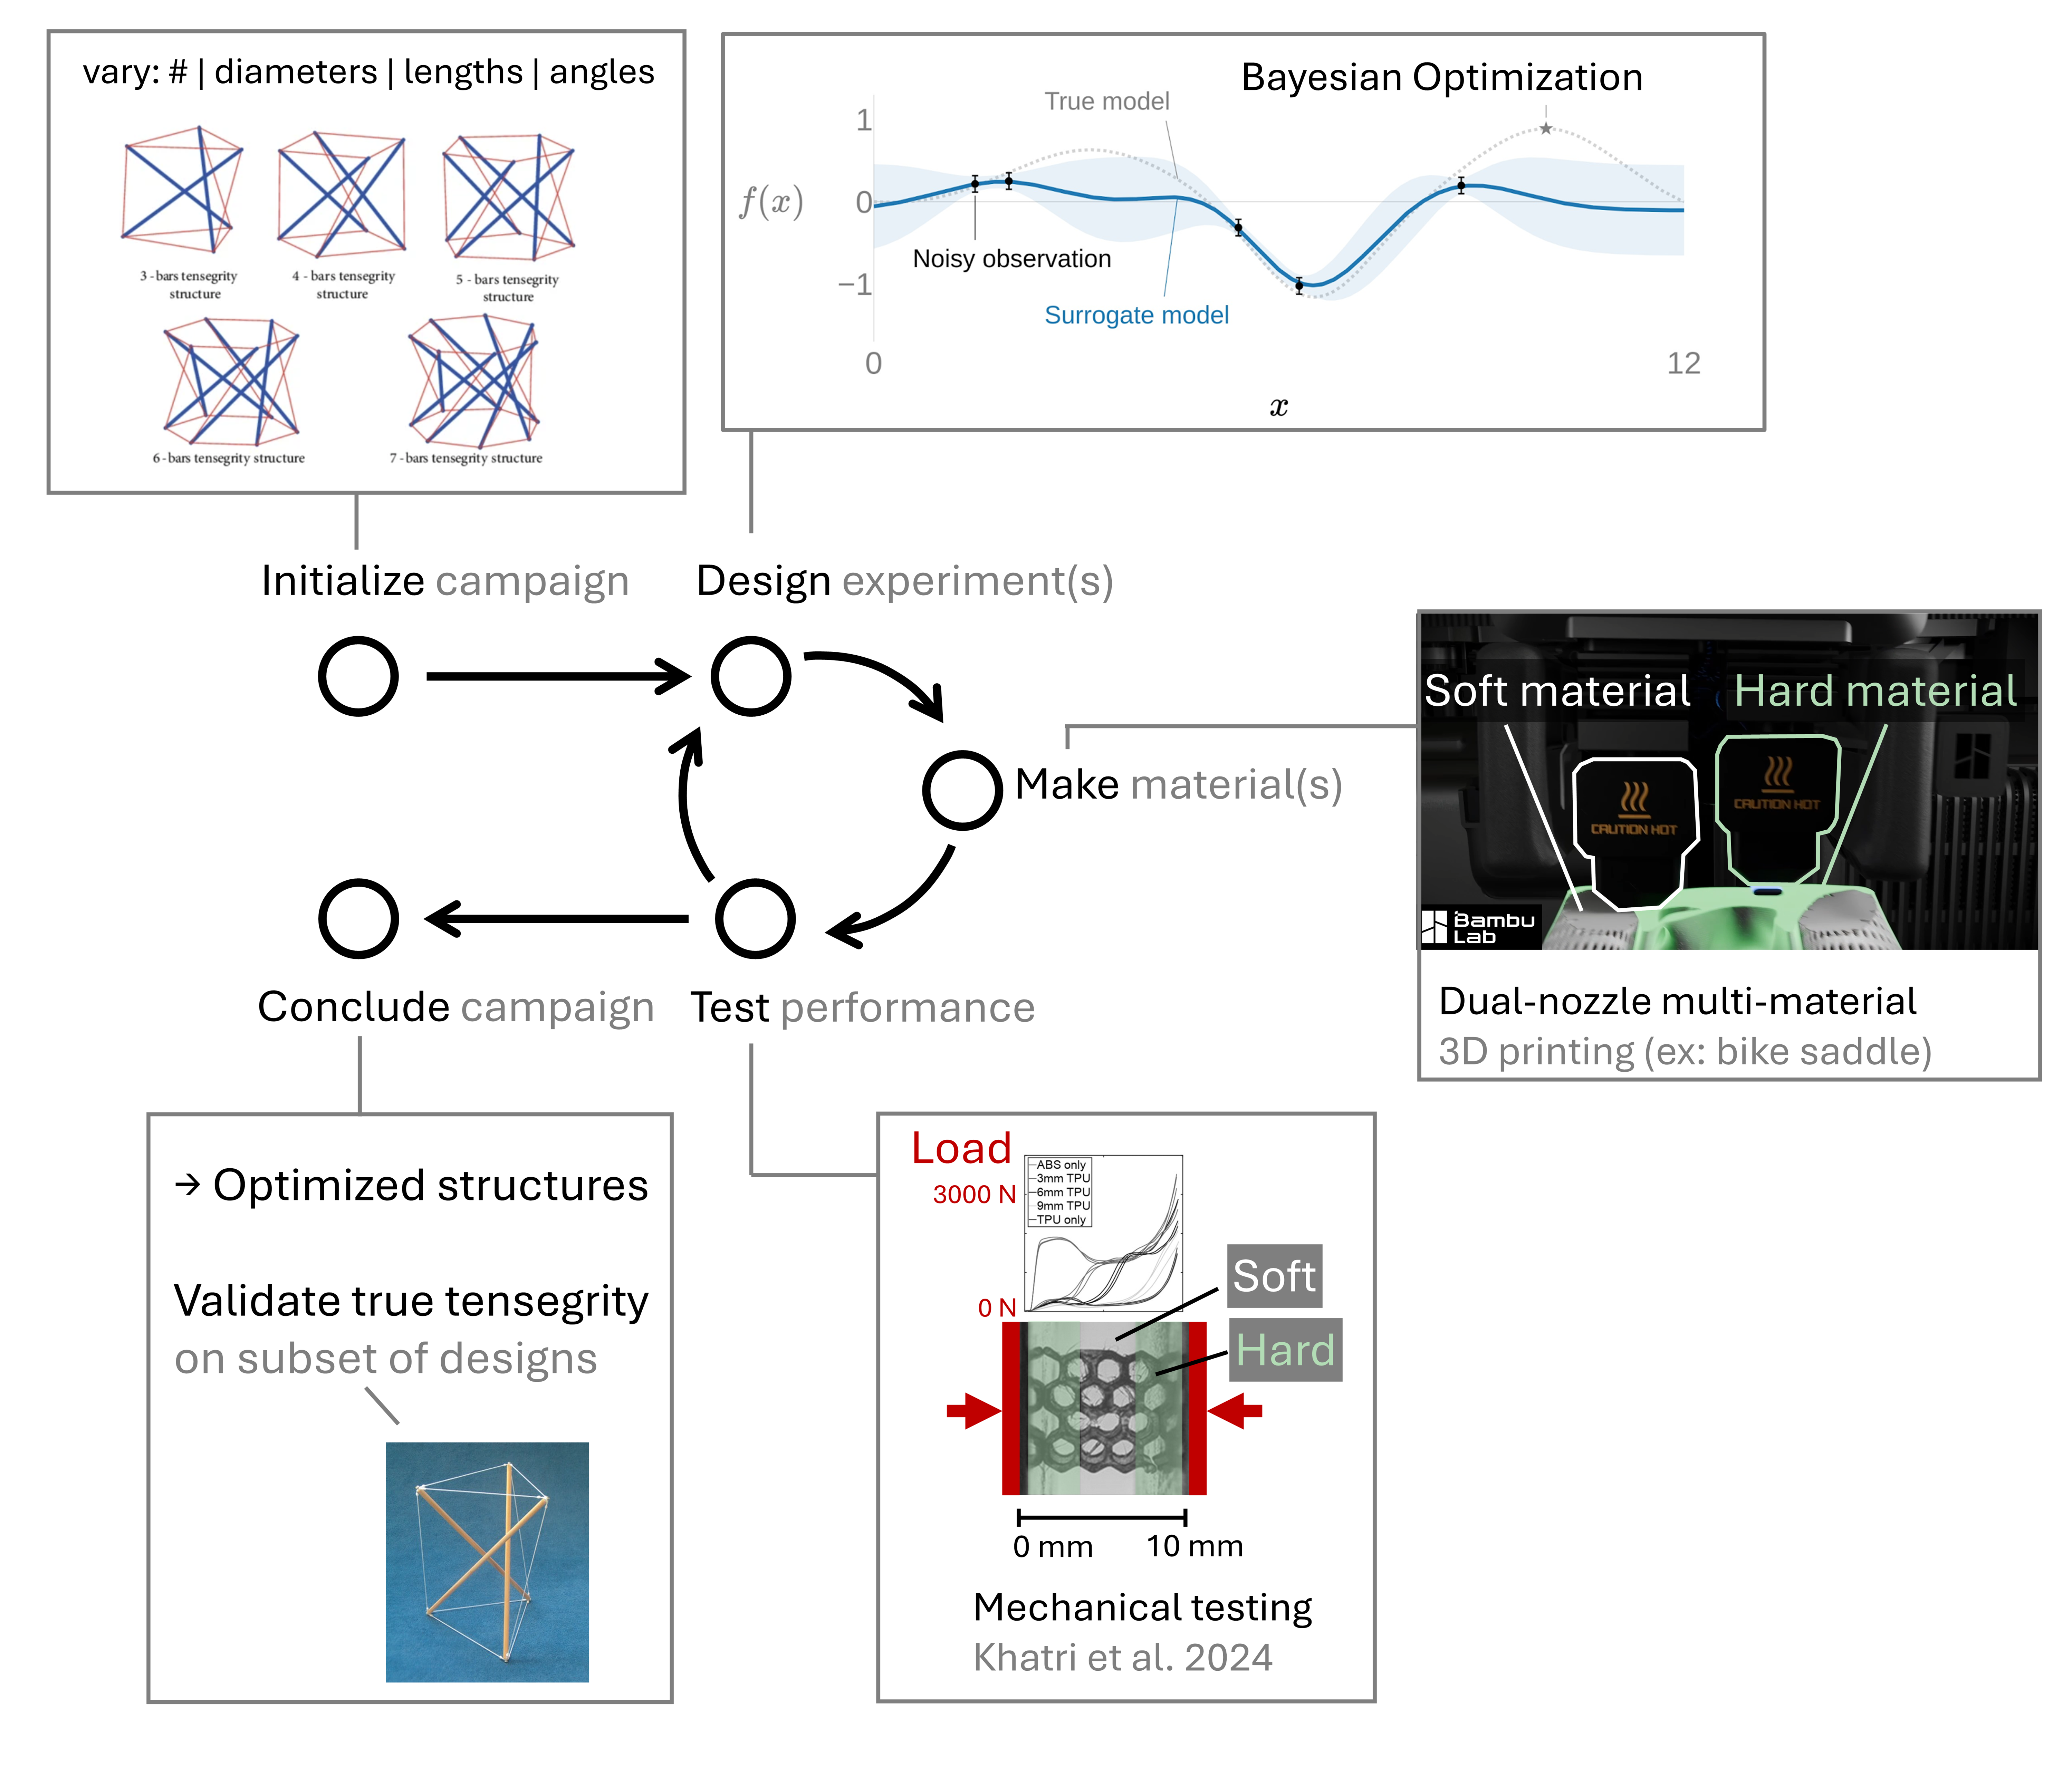
\includegraphics[width=0.7\textwidth]{../figures/overview-updated.png}
  \caption{Closed-loop, experiment-driven design framework. Parameterized
    PLA/TPU tensegrity-inspired unit cells are printed, characterized by
    repeated instrumented drop-weight impacts, and the resulting
    performance data drive a Gaussian-process surrogate that recommends the
    next batch of designs to fabricate.}
  \label{fig:overview}
\end{figure*}%
\todo{Eventually switch this overview figure to a vertical orientation; it is
  currently reproduced from the MRG proposal
  (\texttt{figures/overview-updated.png}).}

The remainder of the paper is organized as follows.
Section~\ref{sec:background} reviews tensegrity mechanics, multi-material
3D printing for energy absorption, and Bayesian optimization with an
emphasis on multi-objective and noise-robust acquisition functions.
Section~\ref{sec:methods} introduces the design parameterization,
fabrication workflow, drop-tower protocol and objectives, and BO loop,
and states the planned metal-analog comparison.
Section~\ref{sec:results} reports all four measured batches, the
surrogate audits, and the replication findings, and
Section~\ref{sec:discussion} discusses the
implications and limitations of the approach. Section~\ref{sec:conclusions}
concludes.

% =============================================================================
\section{Background}
\label{sec:background}
% =============================================================================

\subsection{Tensegrity-Inspired Architectures for Energy Absorption}

Tensegrity prisms and their planar extensions exhibit
softening-stiffening response under
compression~\citep{amendola2014experimental, zhang2018tensegrity,
fraternali2015tensegrity}, characteristics desirable for impact
mitigation because the structure can absorb a large fraction of the
input energy at a controlled, sub-injurious force plateau.
Santos~\cite{santos2023towardanovel} recently characterized a tensegrity
energy-dissipation metamaterial reporting equivalent viscous damping
on the order of $\sim$23\% with negligible residual strain per impact,
underscoring the suitability of tensegrity-inspired architectures for
repeated-impact use cases.
The space program literature documents large-scale tensegrity-inspired
absorbers for planetary landing~\citep{agogino2018superball,
caluwaerts2014superball, sabelhaus2015system, vespignani2018design,
deitrich2022titan} and a long history of crushable energy-absorbing
landing systems~\citep{cloutier1966landing, adams2004merairbag,
jackson2014honeycomb}. Pajunen et~al.~\cite{pajunen2019design} demonstrated that
truncated-tetrahedral tensegrity-inspired unit cells can be directly
3D-printed and exhibit load-limiting plateaus, motivating the present
focus on additively manufactured TPU/PLA composites.
More recent work on dynamically loaded additively-manufactured
energy-absorbing lattices~\cite{davami2019dynamicenergyabsorption}, together
with Intrigila et~al.'s bistable tensegrity-like unit cell for lattice
metamaterials~\cite{intrigila2022fabricationandexperimental} as the closest
published analog, confirms that this architecture class also responds favorably
under impact and quasi-static loading, although neither study employed
multi-material FDM or closed-loop design optimization.
Table~\ref{tab:novelty} situates the present work against selected
prior efforts spanning the three elements combined here (impact-tested
printed tensegrity-inspired structures, rigid-flexible fabrication,
and BO of architected materials), making explicit that, among the
studies reviewed, no single prior study combines a multi-material FDM
tensegrity-inspired architecture with an \emph{experiment}-driven
optimization loop.

\begin{table*}[t]
  \centering
  \caption{Positioning of this work against selected prior efforts
    spanning the elements combined here. The present campaign uses
    physical drop measurements of the transmissibility ($t_{180}$)
    and a mass-weighted rebound energy score ($E_{\mathrm{reb}}$)
    as its BO responses; it does not optimize specific energy
    absorption or crush energy.}
  \label{tab:novelty}
  \footnotesize
  \setlength{\tabcolsep}{4pt}
  \begin{tabular}{@{}llllll@{}}
    \toprule
    Study & Architecture & Fabrication & Optimization & Response optimized & Ground truth \\
    \midrule
    Pajunen et~al.\ 2019~\cite{pajunen2019design}
      & Truncated-tetrahedral & Single-material & None & n/a & Experiment \\
      & tensegrity-inspired & 3D print & (single condition) & & (drop impact) \\[2pt]
    Intrigila et~al.\ 2022~\cite{intrigila2022fabricationandexperimental}
      & Bistable tensegrity-like & Single-material & None & n/a & Experiment \\
      & lattice unit cell & 3D print & & & (quasi-static compr.) \\[2pt]
    Mo et~al.\ 2023~\cite{mo2023accelerated}
      & Architected lattices & n/a (simulation) & Multifidelity BO & Simulated response & Simulation \\
      & & & & metric & (+ sparse high-fid.) \\[2pt]
    Almeida 2025~\cite{almeida2025highstrainrate};
      & Tensegrity-inspired & Additive & None reported & n/a & Experiment \\
    \ \ Davami 2025~\cite{davami2025dynamicanalysis}
      & structures & manufacturing & & & (high-rate/dynamic) \\[2pt]
    Wang et~al.\ 2026~\cite{wang2026integrated}
      & Tensegrity-inspired & Integrated & None reported & n/a & Physical \\
      & rigid-flexible metamat. & dual-material & & & validation \\[2pt]
    \textbf{This work}
      & Tensegrity-inspired & Multi-material & Experiment-driven & $t_{180}$; provisional & Physical \\
      & $T_3$-prism cell (PLA/TPU) & FDM (PLA + TPU) & BO (SAASBO/qNEHVI) & $E_{\mathrm{reb}}$ & experiment \\
    \bottomrule
  \end{tabular}
\end{table*}


\subsection{Multi-Material 3D Printing of PLA/TPU Composites}

Multi-material rigid-soft FDM enables stiff/compliant combinations on a
single platform with tunable energy absorption, demonstrated for thick-panel
origami with PLA (or ABS/CFRP) panels and TPU hinges~\cite{ye2023multimaterial}
and for ABS-TPU honeycombs~\cite{khatri2024energy}. Neither study is itself a
tensegrity, but both establish the rigid-soft co-printing route we adopt. Ye
et~al.~\cite{ye2023multimaterial}
introduced a \emph{wrapping-based} strategy in which rigid cores are
encapsulated by continuous soft skins, reported to reduce interface
delamination under cyclic loading, something we take inspiration from in our
designs.
Beyond these rigid-soft demonstrations, a growing body of work confirms
that genuinely tensegrity-inspired architectures can be additively
manufactured and exhibit programmable mechanical response. Bauer
et~al.~\cite{bauer2021tensegrity} showed that 3D-printed tensegrity
metamaterials delocalize deformation to resist catastrophic failure, while
Pajunen et~al.~\cite{pajunen2021prestrain} tuned acoustic bandgaps in
3D-printed tensegrity-inspired lattices through prestrain, and
Sabouni-Zawadzka et~al.~\cite{sabounizawadzka2024experimental}
experimentally characterized 3D-printed tensegrity-inspired metamaterials
built on the simplex module. More directly relevant to impact, Almeida
et~al.~\cite{almeida2025highstrainrate} and Davami
et~al.~\cite{davami2025dynamicanalysis} characterized the high-strain-rate
and dynamic response of additively manufactured tensegrity-inspired
structures, and Wang et~al.~\cite{wang2026integrated} reported an
integrated fabrication-and-validation workflow for tensegrity-inspired
rigid-flexible metamaterials. Collectively these studies establish the
additive-manufacturability, tunability, and impact relevance of the
architecture class adopted here, none combining multi-material FDM with an
experiment-driven optimization loop.
Recent multi-material PLA/TPU sandwich and layered
composites~\citep{arifvianto2022mechanicalpropertiesof} report
quantitative bounds on
stiffness, strength, and energy absorption for the same PLA-TPU pair
used here, while FDM PLA fatigue
data~\citep{ezeh2018onthefatigue, vanaei2021multiscaledamageanalysis}
inform conservative design bounds for the rigid struts.
Architected multi-material lattices with co-printed compliant skins
have been explicitly designed for high specific energy
absorption~\citep{yavas2022designandfabrication}; recent surveys catalogue the
rapidly expanding additively manufactured polymeric energy-absorption
literature~\citep{bustihan2026recentadvancesin,
liu2026threedimensionalprintedlattice}. \todo{Add a short paragraph on
relevant TPU/PETG tensegrity search-space bounds once the Edison
literature task \texttt{5ae24eaf-5b6e-45cf-9f6c-1c7fbd881738}
synthesis is integrated.}

\subsection{Bayesian Optimization for Architected-Material Design}

Bayesian optimization is a sequential, model-based strategy for
optimizing expensive black-box functions using a Gaussian-process
surrogate~\citep{shahriari2016taking, frazier2018tutorial}. Modern
implementations such as BoTorch~\citep{balandat2020botorch} and the Ax
platform built atop it~\citep{pmlr-v293-olson25a} support
parallel batched evaluations and a wide variety of acquisition
functions; recent algorithmic advances include log-EI for numerical
robustness~\citep{ament2023logei}, noisy expected hypervolume
improvement for multi-objective settings~\citep{daulton2021nehvi},
input-noise-robust acquisitions~\citep{daulton2022robust}, and
evolution-guided constrained multi-objective BO for self-driving
labs~\citep{low2024evolution}. Mixed/categorical search spaces, needed
for the planned connectivity-topology extension rather than the
continuous $T_3$-prism prototype studied here, have dedicated
treatments in BOCS~\citep{baptista2018bocs} and the
one-hot-with-rounded-kernel construction
of~\citep{garridomerchan2020dealingwithcategorical}. BO has been
applied to architected-material
design~\citep{mo2023accelerated}
and to additive manufacturing~\citep{zhang2021bo}.
Mo et~al.~\cite{mo2023accelerated} in
particular established a multifidelity BO framework for architected
materials by fusing low-fidelity simulations with high-fidelity
ground truth via nonlinear information-fusion
priors~\citep{perdikaris2017nonlinear}; the present work shifts the
emphasis from simulation surrogates to direct experimental data,
appropriate for materials whose constitutive response is difficult to
calibrate from first principles.

% =============================================================================
\section{Materials and Methods}
\label{sec:methods}
% =============================================================================

\subsection{Design Parameterization}
\label{sec:methods:parameterization}

We parameterize a family of tensegrity-inspired unit cells via four
groups of design variables. For the working $T_3$-prism prototype that
defines the initial BO search space (Section~\ref{sec:methods:bo}),
only the first two groups are active and all of their variables are
\emph{continuous}; the connectivity-topology and tiling groups are
held fixed for this prototype and are listed here as planned
extensions of the design family:
\begin{itemize}
  \item \textbf{PLA compression members.} Strut diameter $d_s$ and
    length $\ell_s$, with the slenderness ratio $\ell_s / d_s$ bounded
    away from buckling-dominated regimes.
  \item \textbf{TPU tension elements.} Cross-sectional area $A_t$ (or
    equivalent diameter $d_t$ for circular cross-sections).
  \item \textbf{Connectivity topology (future extension).} Selected
    from a discrete set of candidate unit cells (e.g.,
    truncated-tetrahedral, prism-based, and octahedral variants); when
    activated, the design vector would encode this as a categorical
    choice. It is held fixed at the $T_3$ prism for the present
    campaign.
  \item \textbf{Unit-cell tiling (future extension).} Number of cells
    $N_x \times N_y \times N_z$ and the orientation of each cell
    relative to the impact direction; held fixed at a single cell here.
\end{itemize}
\todo{Specify exact manufacturing-feasibility constraints once
finalized; the connectivity-topology categorical encoding is deferred
until that variable is activated beyond the $T_3$ prism.}

\paragraph{Working prototype and search-space evolution} The first
instance of this family used to validate the fabrication and test
pipeline is a three-strut, $T_3$-prism-inspired cell scaled to a
$\sim$50\,mm bounding box. In batches 1 and 2 the BO harness exposes
five continuous design variables (base radius $R$, cell height $H$,
twist angle $\theta$, a single strut diameter $d_s$, and a single
cable (tendon) diameter $d_t$) over the ranges listed in
Table~\ref{tab:design-vars}; the cable diameter $d_t$ is treated as a
\emph{continuous} variable on $[3.0, 5.5]$\,\si{mm} rather than a
discrete set. From batch 3 the space grows to include the print
process: two per-article sparse-infill densities (strut and tendon,
each 12 to 35\%) chosen by the acquisition for every article, and
four filament settings (PLA and TPU nozzle temperature and maximum
volumetric speed) that are physically one value per print job, so
they are drawn as one quasi-random point per batch and are
acknowledged as confounded with batch until a round varies them
within a plate (Section~\ref{sec:methods:bo}). Under the prism's
$D_3$ symmetry all struts share one diameter and all cables share one
diameter, so the parameterization uses a single strut-diameter axis
and a single cable-diameter axis (two member-diameter axes), leaving
room to relax to per-orbit (saddle, top, bottom) or fully per-member
diameters once the individual orbits have been characterized.\todo{Cite the
heterogeneous-parameters Edison LITERATURE\_HIGH brief
(\texttt{5191cf4d}) on $D_3$-symmetric vs.\ fully-per-member
parameterization.} The joint diameter $d_j$ is held fixed at
\SI{7.0}{mm} rather than optimized: it sets the printed strut-end cage
that houses the internal cable anchors
(Section~\ref{sec:methods:fabrication}), so it is constrained primarily by the
TPU-tendon outlet count and the dual-nozzle clearance rather than by
energy-absorption performance, and fixing it keeps the anchor geometry
constant across specimens so that the optimized variables are not
confounded by joint-strength changes; relaxing $d_j$ is deferred to a
follow-on joint-design study. Figure~\ref{fig:printed-prototypes}
shows the parametric CAD model alongside an as-printed prototype of this
working $T_3$ prism.

\paragraph{Constant-mass projection and printability screens} Because
cell mass varies severalfold across the raw design box, an
unconstrained search would partly reward designs for carrying more
material rather than for their architecture. Every candidate is
therefore projected onto a constant material budget before printing:
the design is uniformly rescaled (all dimensions except the twist
angle) until its mass target is met, converged to within
\SI{0.15}{g} on rendered geometry. The target evolved with the
campaign. Batches 1 and 2 held \emph{solid} CAD mass
$\rho_{\mathrm{PLA}} V_{\mathrm{PLA}} + \rho_{\mathrm{TPU}}
V_{\mathrm{TPU}}$ at $m^{\star} = \SI{30.95}{g}$, the solid mass of
the reference prism. That budget does not hold printed grams
constant, because PLA struts print at partial infill while thin TPU
cables print near solid: as-printed masses spanned
\SIrange{18.50}{22.04}{g} across the tested seed articles
(coefficient of variation 5.5\%) and \SIrange{17.91}{23.47}{g}
(8.7\%) across batch 2, so the abstract's ``common mass budget'' is
approximate for those batches and the surrogate carries each
article's weighed mass explicitly
(Section~\ref{sec:methods:bo}). From batch 3 the projection instead
holds \emph{printed} mass at \SI{20.23}{g} (the reference article's
weight) by inverting the calibrated printed-mass model described in
the Supplementary Information; the achieved batch mass CVs were
1.7\% (batch 3) and 2.3\% (batch 4). Two printability screens are
evaluated on the projected geometry and recorded as flags rather
than hard rejections: a cylindrical build envelope
$\pi R^2 H \le \SI{250}{cm^3}$ and the \SI{3.0}{mm} TPU
self-bridging floor on the as-projected cable diameter (the
projection can scale a nominally feasible cable below the floor; the
two seed designs where this occurred both exhibited tendon stringing
defects, consistent with the screen, and the batch-4 attenuators
printed at 2.5 to \SI{2.8}{mm} with only minor stringing, so the
floor is a defect predictor rather than a hard failure line).

\begin{table}[ht]
  \centering
  \caption{Design variables for the $T_3$-prism campaign, as implemented
    in the BO harness. The seed batch is an $n=9$ Sobol draw (fixed
    seed) over the five geometry variables, with each design then
    projected onto the constant-mass budget of the text. The process
    variables joined the space in batch 3: the two infill densities
    are acquisition-chosen per article, while the four filament
    settings admit one value per print job and are therefore drawn as
    a single quasi-random point per batch (confounded with batch
    until varied within a plate). The joint diameter is held fixed.
    All specimens print in the vertical orientation on a Bambu
    Lab~H2D: one specimen per named build plate in the seed batch,
    one nine-article plate per batch thereafter.}
  \label{tab:design-vars}
  \small
  \begin{tabular}{@{}llccc@{}}
    \toprule
    Variable & Symbol & Units & Range & Active \\
    \midrule
    Base radius            & $R$       & mm  & 25-40 & batch 1 on \\
    Cell height            & $H$       & mm  & 60-110 & batch 1 on \\
    Twist angle            & $\theta$  & deg & 40-80 & batch 1 on \\
    Strut (PLA) diameter   & $d_s$     & mm  & 6.0-12.0 & batch 1 on \\
    Cable (TPU) diameter   & $d_t$     & mm  & 3.0-5.5 & batch 1 on \\
    Strut infill density   & -        & \%  & 12-35 & batch 3 on \\
    Tendon infill density  & -        & \%  & 12-35 & batch 3 on \\
    PLA nozzle temperature & -        & \si{\celsius} & 212-228 & batch 3 on\textsuperscript{a} \\
    PLA volumetric speed   & -        & \si{mm^3/s} & 20-30 & batch 3 on\textsuperscript{a} \\
    TPU nozzle temperature & -        & \si{\celsius} & 235-245 & batch 3 on\textsuperscript{a} \\
    TPU volumetric speed   & -        & \si{mm^3/s} & 2.2-3.6 & batch 3 on\textsuperscript{a} \\
    Joint diameter (fixed) & $d_j$     & mm  & 7.0 & - \\
    \bottomrule
  \end{tabular}\\[2pt]
  {\footnotesize \textsuperscript{a}One value per print job (a plate
  carries a single filament configuration), so per-batch rather than
  per-article.}
\end{table}%
\todo{The cable-diameter lower bound (3.0\,mm) is set by the Bambu
  auto-support detection floor; add the remaining
  manufacturing-feasibility constraints once finalized.}

\paragraph{As-built resolution of the continuous variables} Although
$d_s$ and $d_t$ are treated as continuous, the as-built cross-sections
are discretized by the nozzle diameter, the slicer line width, and
support interaction, so the effective search granularity is coarser
than the nominal continuous box. The realized member diameter therefore
changes in steps set by the line-width quantization rather than
continuously, and the smallest CAD change that yields a reliably
distinguishable as-built member is bounded below by these slicer
limits; the lower TPU-tendon bound (\SI{3.0}{mm}) is itself a
workflow-specific limit tied to the TPU self-bridging and auto-support
detection floor on this H2D platform rather than a fundamental
geometric one. The as-built quantity measured for every article is its
mass, weighed on a \SI{0.01}{g} scale; dimensional metrology of the
printed members has not yet been performed, so the geometry attached
to the surrogate is the commanded post-projection geometry. Two
print-to-print measurements bound the fabrication scatter: one seed
design printed in triplicate has a mass standard deviation of
\SI{0.457}{g}, and the full reprint of the batch-3 plate produced
nine design-replicate mass pairs whose second print weighed
\SI{0.27}{g} heavier article for article on average, a per-session
flow offset rather than random scatter. Both feed the observation
noise model (Section~\ref{sec:methods:bo}).

\begin{figure}[t]
  \centering
  \begin{subfigure}[b]{0.42\linewidth}
    \centering
    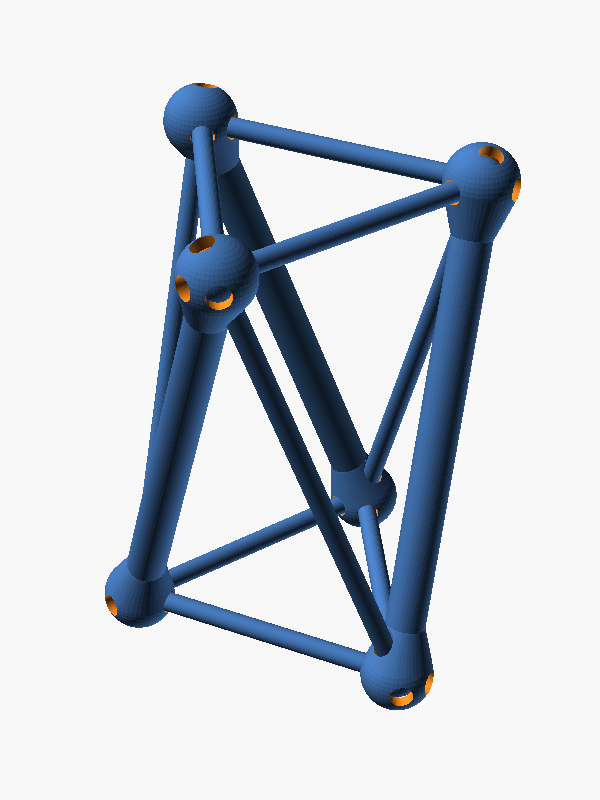
\includegraphics[width=\linewidth]{../figures/photos/cad-render.png}
    \label{fig:proto-cad}
  \end{subfigure}\hfill
  \begin{subfigure}[b]{0.54\linewidth}
    \centering
    \begin{tikzpicture}
      \node[anchor=south west,inner sep=0] (ph)
        {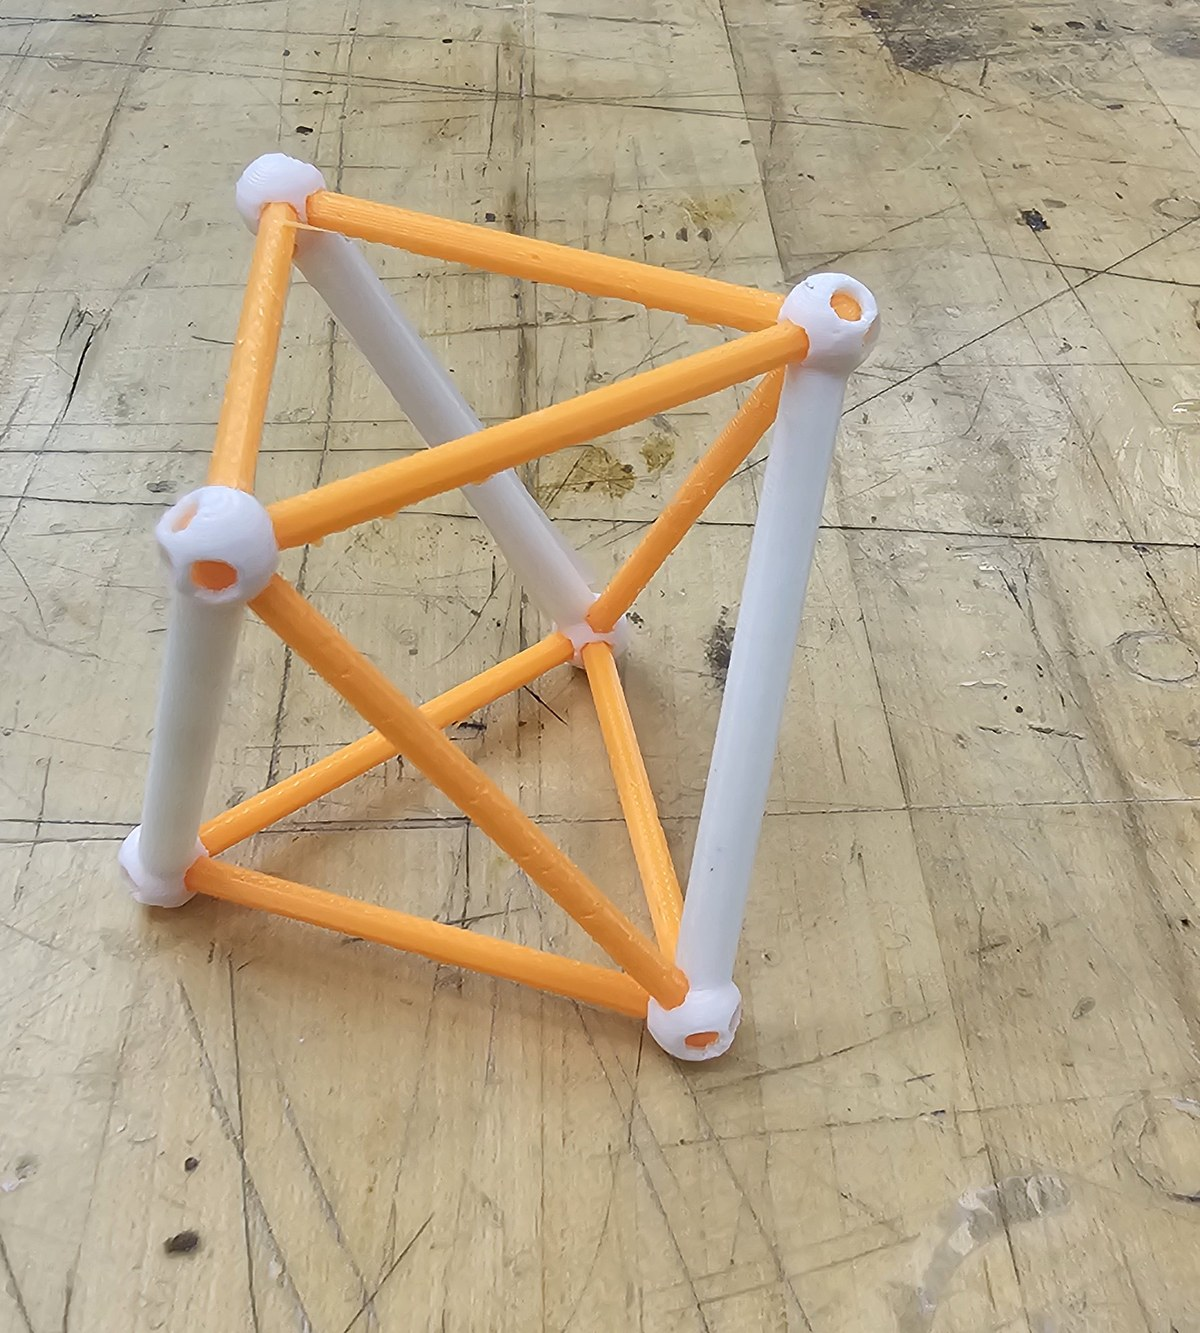
\includegraphics[width=\linewidth]{../figures/photos/printed-specimen.jpg}};
      \begin{scope}[x={(ph.south east)},y={(ph.north west)},
                    font=\sffamily\scriptsize]
        \tikzset{callout/.style={-{Latex[length=1.5mm]},line width=0.5pt,
                                 draw=red!75!black}}
        \tikzset{lab/.style={fill=white,fill opacity=0.85,text opacity=1,
                             inner sep=1pt,rounded corners=1pt}}
        \draw[callout] (0.74,0.95) node[lab,anchor=south]{$d_s$}
          -- (0.63,0.52);
        \draw[callout] (0.22,0.96) node[lab,anchor=south]{$d_t$}
          -- (0.34,0.70);
        \draw[{Latex[length=1.5mm]}-{Latex[length=1.5mm]},line width=0.5pt]
          (0.05,0.23) -- (0.05,0.85) node[lab,midway]{$H$};
      \end{scope}
    \end{tikzpicture}
    \label{fig:proto-print}
  \end{subfigure}
  \caption{Working $T_3$-prism prototype. \emph{(a)} Parametric OpenSCAD model
    whose base radius $R$, cell height $H$, twist angle $\theta$, strut diameter
    $d_s$, and cable diameter $d_t$ are the design variables of
    Table~\ref{tab:design-vars}. \emph{(b)} A representative dual-material print
    from the PR~\#35 print history (rigid PLA struts, here in white; tendon
    members in orange), with callouts marking the strut diameter $d_s$, a tendon
    (cable) diameter $d_t$, and the cell height $H$; the inter-plate twist
    $\theta$ is the relative rotation of the top and bottom node triangles, and
    the base radius $R$ sets their circumradius.}
  \label{fig:printed-prototypes}
\end{figure}

\subsection{Multi-Material Fabrication}
\label{sec:methods:fabrication}

Specimens are fabricated on a multi-material FDM printer using PLA for
the rigid struts and TPU for the soft tension elements.
Figure~\ref{fig:fab-workflow} summarizes the end-to-end fabrication and
characterization workflow, from parametric CAD through multi-material
slicing, dual-extrusion printing, post-processing, and mechanical
testing. Rather than
wrapping the struts in a continuous TPU skin, the current design anchors
the TPU tension elements \emph{inside} the ends of each PLA strut: the
cables converging at a given strut end are joined within the strut,
which acts as a rigid cage housing the junction, and the individual
tendons then exit through discrete outlets. This keeps the soft-rigid
interface in internal, compression-dominated pockets rather than at an
exposed overmolded surface. This construction effectively inverts the
material roles of Ye et~al.'s soft-skin-over-rigid-core
wrapping~\cite{ye2023multimaterial}: here a soft TPU core is captured within
a rigid PLA shell, so we cite that work only as a multi-material co-printing
precedent rather than as validation of the present junction. \todo{Quantitatively
verify the internal-anchoring junction strength against the PR~\#39 / PR~\#35
joint pull-out studies before making any cyclic-durability claim.} \todo{Document slicer profile
(layer height, infill, print speed, nozzle temperatures, retraction
settings) and validation prints used to characterize PLA-TPU interface
strength.}

\paragraph{Print platform and joint geometry} The working platform is
a Bambu Lab~H2D printer, which permits a single rigid-soft build
without filament swaps. Strut endpoints are tied to cables through
parametric joint geometries developed and ranked through a five-design
OpenSCAD study (anchor-bulb, dovetail, TPU-sleeve overmold,
eyelet-loop, and TPU-rebar variants); the working prototype uses a
dovetail joint (Design~B) with an anchor-bulb backup (Design~A) for
sensitivity studies, with a captive TPU core routed inside the PLA
shell to keep the soft tendon protected from layer-line failure at
the strut-to-cable transition. The full five-design comparison and the
selected junction are detailed in the Supplementary Information.\todo{Cite the
joint-design Phase-3 CAD review (Edison ANALYSIS \texttt{19e0c868}) and the
Phase-4 vision review (\texttt{e9a1f4cc}) once both are integrated into the
references.}

\paragraph{Supports for soft members} Because near-vertical TPU
tendons are otherwise unsupported during printing, automatic support
generation is disabled and supports are painted manually in the
slicer: PLA edge supports run along each tendon, with the
support-to-object clearance tightened from \SI{0.35}{mm} to
\SI{0.2}{mm} during tuning on the reference prism. Two support-removal
artifacts recur in the seed batch (surface stringing and, on two
articles, TPU strands pulled off bottom tendons during support
removal) and are logged per article in the print key (Supplementary
Information). An automated alternative (a lowered support-threshold
angle plus mesh-ray-cast narrowing pillars) was developed in parallel
and is documented in the Supplementary Information.

\paragraph{Moisture and nozzle management} TPU is hygroscopic, so the
soft filament is fed from a heated dry box held near \SI{8}{\percent}
relative humidity, logged per print. Midway through the seed batch the
TPU extruder developed a progressive flow taper (a partial clog,
compounded by a stray PLA fragment found inside the extruder); it was
resolved by a cold pull and by moving the TPU to a dedicated
high-flow \SI{0.6}{mm} nozzle, after which print quality was restored.
The affected and post-fix articles are identified in the print key so
that any nozzle-related covariate can be checked against the measured
objectives.

\begin{table}[ht]
  \centering
  \caption{Multi-material print parameters on the Bambu Lab~H2D,
    transcribed from the archived as-printed Bambu Studio project
    (\texttt{t3-prism-bo-batch.H2D-MM-PLAstruts-TPUcables.as-printed.3mf},
    Bambu Studio 2.7.1). Filaments are Bambu Lab PLA Basic (struts,
    support material) and Bambu Lab TPU~85A (tendons); the print
    profile is ``0.30\,mm Standard @BBL H2D 0.6 nozzle.'' The
    reporting structure follows the methods section of Ye
    et~al.~\cite{ye2023multimaterial}.}
  \label{tab:print-params}
  \small
  \setlength{\tabcolsep}{3pt}
  \begin{tabular}{@{}lcc@{}}
    \toprule
    Parameter & PLA (struts) & TPU 85A (tendons) \\
    \midrule
    Nozzle                             & \SI{0.6}{mm} & 0.4 then \SI{0.6}{mm} HF\textsuperscript{a} \\
    Nozzle temperature (\textdegree C) & 220 & 220 \\
    Bed temperature, profile (\textdegree C) & 55 & 35 \\
    Layer height / line width (mm)     & \multicolumn{2}{c}{0.30 / 0.62} \\
    Infill                             & 15\% grid, 2 walls & near-solid \\
    Outer / inner wall speed (mm/s)    & \multicolumn{2}{c}{200 / 300 (profile)} \\
    Filament drying                    & n/a & dry box, $\sim$8\% RH \\
    Build-plate type                   & \multicolumn{2}{c}{Textured PEI} \\
    Build orientation                  & \multicolumn{2}{c}{Vertical} \\
    Supports                           & \multicolumn{2}{c}{Manual painted tree supports, PLA} \\
    \bottomrule
  \end{tabular}\\[2pt]
  {\footnotesize \textsuperscript{a}The TPU side ran a standard
  \SI{0.4}{mm} nozzle until the mid-batch clog, then a dedicated
  high-flow (HF) \SI{0.6}{mm} nozzle; affected articles are flagged in
  the print key.}
\end{table}%
\todo{@achris0520 to confirm the physical nozzle hardware (the
  archived as-printed project records \SI{0.6}{mm} on both extruders,
  consistent with the post-fix state; the TPU side ran \SI{0.4}{mm}
  before the mid-batch nozzle change logged in the print key) and to
  supply filament lot numbers and drying duration, which the slicer
  archive does not record.}

\begin{figure*}[t]
  \centering
  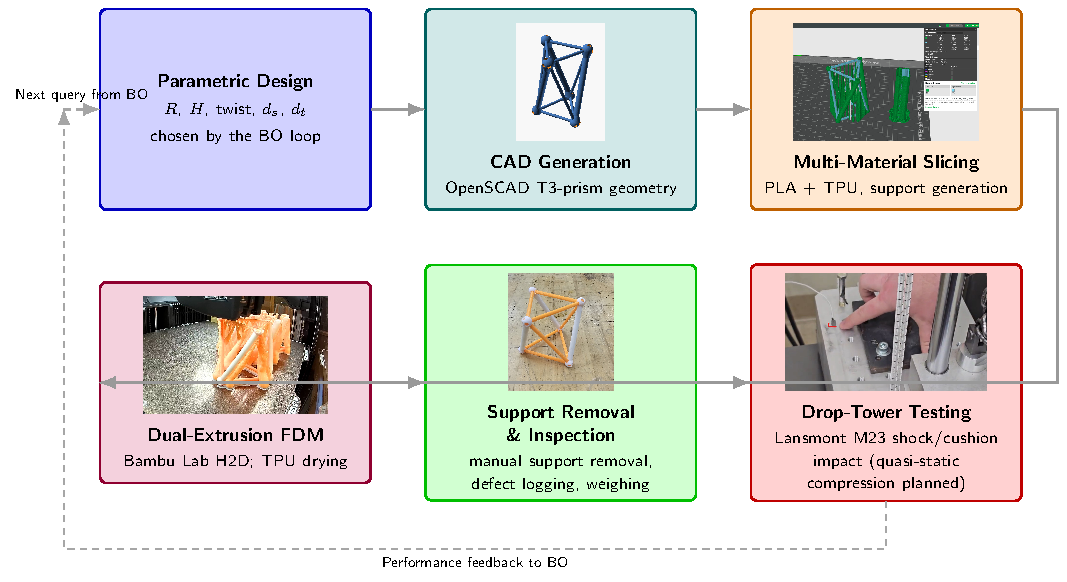
\includegraphics[width=\textwidth]{../figures/fab-workflow.pdf}
  \caption{Fabrication and characterization workflow for the multi-material
    tensegrity-inspired unit cells: design parameters drive parametric CAD,
    slicing with manually generated TPU supports, a single multi-material
    print on the Bambu Lab~H2D, post-processing and inspection, and
    mechanical testing. Node photographs are representative artifacts drawn
    from the project's build history: the OpenSCAD $T_3$-prism render
    (CAD), the dual-nozzle Bambu Studio slice with PLA on the left extruder
    and TPU on the right (slicing), an in-progress H2D print of the prism
    batch (FDM), an as-printed specimen (post-processing), and the
    bungee-assisted drop-tower base plate with accelerometer (testing).}
  \label{fig:fab-workflow}
\end{figure*}%

\subsection{Experimental Characterization}
\label{sec:methods:testing}

\paragraph{Drop-tower fixture} The primary characterization is
repeated drop-weight impact on a Lansmont Model~23 shock test system.
The printed specimen rides upright on the carriage plate, which is
raised \SI{60}{in} (\SI{1.524}{m}) along guide rails and released; the
plate lands on a single \SI{0.5}{in} Shore 60~OO polyurethane cushioning
sheet, which shapes the landing into a single sharp base pulse of
roughly \SI{1.6}{ms} duration. This impact-surface configuration was
selected by a blinded crossover experiment over three candidate mat
arrangements, and unlike a felt stack it does not measurably compact
over hundred-drop sessions. Rig health is monitored continuously
through the impact velocity change $\Delta v$ recovered from the base
accelerometer: over an uninterrupted 100-drop characterization session
the $\Delta v$ coefficient of variation was 0.54\% with no drift, and
every campaign session is checked against the healthy tower baseline
(details, including the within-session mat warm-up and recovery
pattern, in the Supplementary Information). One drop takes roughly
\SI{42}{s}, so a seed-batch characterization completes in about
ninety minutes per article and a later-batch session in about
fifteen.

\paragraph{Instrumentation and signal processing} A single-axis
piezoelectric accelerometer on the carriage plate records the base
input and triggers the acquisition; a triaxial accelerometer (Dytran
3133A4) seated in a printed pocket at the specimen's top vertex records
the transmitted response. The two base-capable channels were
cross-calibrated in place over fifteen co-located drops (ratio
$0.953 \pm 0.001$ at matched filtering), and the transducer settings
are archived with the data. Signals are captured at
\SI{1.25}{MHz} over a \SI{100}{ms} record with a \SI{2}{ms}
pre-trigger. All channels are low-pass filtered with the SAE~J211/1
channel-frequency-class (CFC) filters~\citep{saej211}, implemented from
the standard's published coefficients with the two-pass corner
frequency handled explicitly (a common implementation shortcut narrows
the passband by roughly 20\%, which we identified and corrected before
the campaign; all reported numbers use the corrected filter). CFC-180
is the reporting class for peak metrics, with CFC-1000 retained as a
higher-bandwidth diagnostic.

\paragraph{Per-article objectives and session protocol} Session
length evolved with the campaign's understanding of its own noise,
and the per-batch counts are stated here because they differ. Seed
sessions recorded 103 drops per article and contribute 101 stabilized
captures each (103 for one article, autv5r) after the first two drops
of each session are discarded as seating warm-up. A pre-campaign
variance study on the commissioning datasets put the statistical
minimum at five stabilized drops after two warm-ups, and the seed
sessions confirmed that the stabilized mean is insensitive to session
length: within-session per-drop CVs of 0.17 to 0.48\% with flat
post-warm-up trends, and a replay of the seed sessions truncated to
twenty drops leaves the transmissibility ranking of all eight tested
articles unchanged, with a worst-case mean shift of $+0.008$ against
design-to-design gaps of 0.007 to 0.087 and a per-drop standard
error still an order of magnitude below those gaps. Later sessions
were therefore shortened to about twenty drops per article: the
committed record lists 21 to 22 valid captures per batch-2 article
and 20 recorded drops per article in batches 3 and 4, against 101
valid captures per seed article, with the first two drops of every
session discarded as before (exact per-session counts are in the
archived per-drop records). The shortening cuts tower time per
article
from about ninety minutes to about fifteen while retaining roughly
four times the minimum stabilized-drop budget; a shorter session
simply enters the surrogate with a proportionally larger standard
error, which the model downweights. The second print-and-test pass
of batch 3
(Section~\ref{sec:results:batches}) subsequently confirmed that
seating and print variation, not session length, limit what a
session can claim, so the freed tower time goes to re-seats. Each
session yields two objectives, each reported as a stabilized mean
with the per-drop scatter quoted as one standard deviation; the
standard error of the mean is what enters the surrogate's noise model
(Section~\ref{sec:methods:bo}):
\begin{equation}
  \begin{aligned}
    t_{180} &\;=\; \frac{\max_t\,\lVert \mathbf{a}_{\mathrm{top}}(t)\rVert_{\mathrm{CFC180}}}
                        {\max_t\,\lvert a_{\mathrm{base}}(t)\rvert_{\mathrm{CFC180}}},\\
    E_{\mathrm{reb}} &\;=\; e_{\mathrm{reb}}\, m\, g\, h,
    \qquad
    e_{\mathrm{reb}} \;=\; \frac{g\, t_{\mathrm{second}}}{2\,\Delta v},
  \end{aligned}
  \label{eq:objectives}
\end{equation}
where $t_{180}$ is the CFC-180 filtered peak-acceleration ratio,
which we name once here and then call the \emph{transmissibility}
throughout: the peak magnitude of the triaxial top-vertex response
over the peak base input within the impact window. The term is used
in the shock-testing sense standard for cushioning and packaging
drop tests, a ratio of filtered peak accelerations across the
article under a single transient, not the steady-state
frequency-response function of vibration isolation: the two peaks
need not be simultaneous, the filter class is part of the
definition, and SAE~J211/1 is cited only for the impact-channel
filtering. Values above unity indicate the structure amplifies the
peak shock reaching its top vertex; values below unity indicate
attenuation. $E_{\mathrm{reb}}$ is a \emph{provisional
mass-weighted rebound score} with units of energy (millijoules per
drop): the dimensionless rebound fraction $e_{\mathrm{reb}}$ is
recovered from the ballistic timing of the top vertex's post-impact
hop~\citep{bernstein1977listening} ($t_{\mathrm{second}}$ is the time
to the second contact event and $\Delta v$ the measured base velocity
change), and it is scaled by each article's own weighed mass $m$ and
the drop height $h$. Two interpretive caveats are deliberate. The
ballistic reading of the second contact event has not yet been
validated against synchronized video, and $\Delta v$ is the base
plate's velocity change rather than a demonstrated incident relative
velocity, so $e_{\mathrm{reb}}$ is a rebound-timing score rather than
a coefficient of restitution; and because a strict restitution reading
would scale returned kinetic energy as the \emph{square} of a velocity
ratio, $E_{\mathrm{reb}}$ is a mass-aware ranking score that penalizes
designs (and grams) that throw more motion back at the payload, not a
measured rebound energy. The score is the campaign's second
objective through all four batches and remains a candidate to become
a constraint once validated
(Section~\ref{sec:discussion}). Using the mass-weighted form rather
than the bare fraction keeps the objective mass-aware: equal fractions
on articles of different printed mass are not equivalent outcomes for
a payload. Ringdown descriptors (the fitted natural frequency $f_n$,
260 to \SI{470}{Hz} for every article but one batch-4 design that
rings at \SI{764}{Hz}, and, where
the exponential fit passes an $r^2 \ge 0.85$ gate, a damping ratio
$\zeta$) are recorded per drop as print-health and prestress
diagnostics~\citep{ashwear2014natural} but are not campaign objectives.
The within-session per-drop CV of $t_{180}$ spans 0.06 to 2.0\%
across the campaign's 35 articles (0.17 to 0.48\% in the seed
batch). These
values describe repeated drops of the same physical article in one
seating and do not estimate print-to-print or seating-to-seating
repeatability; serial dependence among drops may also make
$s/\sqrt{n_{\mathrm{drops}}}$ optimistic. Two replication
measurements bound what a single session can claim: the seed
attenuator re-measured across a day and an independent re-seat
agreed to 0.13\%, while a full second print-and-test pass of the
batch-3 plate showed same-design shifts with a median of $+1.2\%$
and heavy tails (Section~\ref{sec:results:batches}). The campaign
therefore adopted a between-seat replication rule: a single-seating
value that would drive a decision (a batch extreme, a claimed
attenuator, a front membership) requires confirmation on an
independent re-seat before it is treated as a design property. A
mechanism-oriented trace figure (processed
deceleration response with event markers keyed to synchronized video
frames) will be generated from archived campaign captures once the
event labels can be supported by synchronized measurements; no such
figure is shown here because none of the required event
synchronization has yet been performed.

\paragraph{Planned quasi-static extension} The drop test loads the
specimens in their elastic regime (the crush lasts 1 to \SI{3}{ms} and
the article recovers), so crush-energy metrics such as specific energy
absorption (SEA) and compaction efficiency are not recoverable from
these captures by any reprocessing. A quasi-static compression
campaign on a benchtop load frame (BYU CB~123 Instron, with a
low-range load cell appropriate to the expected cell stiffness)
is planned to supply the complementary crush metrics
\begin{equation}
  \mathrm{SEA} \;=\; \frac{1}{m}\!\int_{0}^{\delta_d}\! F(\delta)\,
  \mathrm{d}\delta,
  \qquad
  \eta_c \;=\; \frac{\int_{0}^{\delta_d}\! F(\delta)\,\mathrm{d}\delta}{F_{\max}\,\delta_d},
\end{equation}
with the densification displacement $\delta_d$ taken at the maximum of
the energy-absorption efficiency curve and $F_{\max}$ the peak force
within $[0,\delta_d]$, following the canonical cellular-solid
treatments~\citep{gibson1997cellular, avalle2001characterization,
tan2005dynamic, michailidis2011establishment} and mirroring the
quasi-static protocol of Pajunen et~al.~\citep{pajunen2019design}.
These metrics are reported as a complementary characterization of
selected designs rather than as objectives of the drop-tower campaign.
Slip resistance and traction at the specimen-to-floor interface,
governed by the tip geometry rather than the internal architecture,
follow ISO 11334-4~\citep{iso11334-4} for walking-aid tips and are out
of scope for the present axial-impact study.

\paragraph{Complementary data streams} High-speed video
(\SI{959}{fps}, three clips per specimen) supplements the
accelerometer data. The camera cannot resolve the millisecond-scale
impact pulse (one to two frames), so the division of labor is
explicit: the accelerometer channels produce the objectives, and video
documents the post-impact rebound and recovery. Synchronized
laser-Doppler vibrometry is reserved for follow-up characterization of
selected designs.

\subsection{Experiment-Driven Bayesian Optimization Loop}
\label{sec:methods:bo}

The optimization loop maintains a Gaussian-process (GP) surrogate over
the design space defined in
Section~\ref{sec:methods:parameterization}. After each round of
physical experiments, the surrogate is refit and an acquisition
function is maximized to recommend the next batch of designs to
fabricate. The campaign is posed as a two-objective minimization:
simultaneously minimize the transmissibility $t_{180}$
and the per-drop rebound energy $E_{\mathrm{reb}}$ of
Eq.~\eqref{eq:objectives}. Both objectives serve the same payload:
$t_{180}$ bounds the peak shock it feels during the impact, and
$E_{\mathrm{reb}}$ penalizes the motion thrown back into it afterward.
The seed data showed an apparent trade-off driven substantially by
the single strongest attenuator, not statistically resolved at seven
mapped articles (Spearman $\rho = -0.39$, $p = 0.38$;
Section~\ref{sec:discussion}); the measured front after four batches
is nondegenerate (its members span both axes), and the rebound axis
remains a candidate to become a constraint once its ballistic
reading is validated.
Implementation
uses the Ax platform~\citep{pmlr-v293-olson25a} over
BoTorch~\citep{balandat2020botorch}, with noisy expected hypervolume
improvement (qNEHVI)~\citep{daulton2021nehvi} as the multi-objective
acquisition. The $T_3$-prism search space is fully continuous,
including the process variables added in batch 3
(Table~\ref{tab:design-vars}), so no categorical
encoding is required; the mixed-search-space constructions
of~\citep{garridomerchan2020dealingwithcategorical} and the BOCS
combinatorial baseline~\citep{baptista2018bocs} remain the route for
the future connectivity-topology categorical rather than part of the
current loop. The input-noise-robust acquisition of Daulton
et~al.~\cite{daulton2022robust} and the evolution-guided constrained
variant of Low et~al.~\cite{low2024evolution} are held in reserve as
contingencies.

\paragraph{Surrogate and noise model} The surrogate is the fully
Bayesian sparse axis-aligned subspace model
(SAASBO)~\citep{eriksson2021saasbo}: a Mat\'ern-5/2 kernel with
automatic relevance determination whose length scales carry strong
sparsity-inducing priors and are marginalized by Markov-chain Monte
Carlo (NUTS) rather than point-estimated; every refit in the
campaign, through the batch-4 ingestion, uses this model with qNEHVI
on top (Ax 0.4 for the early rounds, Ax~0.5.0 from the batch-3
refit). We retain SAASBO even though the
dimensionality is modest because marginalizing the hyperparameters
tends to improve uncertainty quantification at the very small sample
sizes of physical campaigns; the fitted model is audited each round
with leave-one-out cross-validation and length-scale-based
sensitivity diagnostics
(Section~\ref{sec:results}). Inputs are normalized to the unit cube
and outputs standardized. Observation noise is supplied per
observation as a fixed variance: for $t_{180}$ the squared standard
error of the stabilized mean,
$\sigma_t^2 = s_{\mathrm{drop}}^2 / n_{\mathrm{drops}}$, and for the
rebound score the drop-scatter term plus the propagated
print-to-print mass scatter,
$\sigma_E^2 = \sigma_{E,\mathrm{drops}}^2 +
(\partial E_{\mathrm{reb}}/\partial m)^2 \sigma_m^2$ with
$\sigma_m = \SI{0.457}{g}$ measured from the one design printed in
triplicate; a shorter session enters with a proportionally larger
standard error. The estimand this noise model implies is the
response of the tested article in its seating, not of a freshly
printed article at the same design: an independent adversarial
review (Section~\ref{sec:discussion}) argued the decision-relevant
target is the latter, and the campaign's response is the measured
replication evidence of Section~\ref{sec:results:batches} (a full
second print-and-test pass of one batch) together with the
between-seat replication rule, rather than an inflated per-article
noise term. SAASBO is the
prespecified surrogate; we make no claim that it outperforms
a standard single-task GP at this dimensionality and sample size,
and the planned head-to-head calibration comparison against a
point-estimated GP with the same kernel remains future work.

\paragraph{Mass treatment} Because the constant \emph{solid}-mass
projection of batches 1 and 2 does not hold printed grams constant
(Section~\ref{sec:methods:parameterization}), printed mass correlates
with the shape variables in the seed batch ($r = 0.83$, $n = 7$,
dominated by the lightest article, against $t_{180}$). The loop
therefore makes mass explicit rather than pretending it away: the
rebound objective is expressed in absolute millijoules using each
article's weighed mass, so added grams are re-penalized through the
energy they deliver back to the payload, while $t_{180}$ deliberately
stays a ratio because payload peak acceleration is a damage criterion
that does not scale with specimen mass. The objective surrogates take
the design coordinates of Table~\ref{tab:design-vars} as their
inputs; printed mass is attached as a separately modeled
\emph{tracking metric}, so the model learns as-printed mass as a
function of the design coordinates and every recommendation reports a
predicted printed mass (the diagnostic refit behind
Fig.~\ref{fig:sensitivity} additionally includes printed mass as an
input, precisely to probe this confound). The calibrated
printed-mass model of the Supplementary Information closed the loop
on this compromise: batches 3 and 4 hold \emph{printed} grams
constant, and the mass-transmissibility correlation across the 26
articles of batches 1 to 3 fell to $r = 0.07$, so the confound the
seed batch raised was broken by design rather than adjusted away in
analysis.

\paragraph{Budget and seeding} The seed batch is an $n = 9$ Sobol
draw with a recorded seed over the five-variable box, printed together
with the fixed reference prism (S0). Optimization proceeds in
sequential batches of $q = 9$ prints, sized to one build-plate
generation cycle. Three model-recommended batches are reported here
(Ax trials 10 to 18, 28 to 36, and 37 to 45; the numbering gap
records a superseded draft batch that was regenerated, before
printing, when the batch-level filament handling was simplified).
From batch 3 the four filament settings take one quasi-random point
per batch, formally the settings of that batch's best-predicted
article, so those axes are confounded with batch and are reported as
unidentified rather than learned. All random seeds,
the full experiment state, and the recommendation tables are recorded
per round; full computational reproducibility (the exact processing
pipeline and model settings) is carried by the campaign code, whose
archival release is a declared submission gate rather than a solved
item. Escalation to
trust-region BO (TuRBO)~\citep{eriksson2019turbo} is planned only if
per-member-diameter extensions push the design space well beyond the
present regime; a single-objective log-Expected-Improvement
run~\citep{ament2023logei} on $t_{180}$ is retained as a baseline for
quantifying the benefit of the multi-objective formulation. The
campaign code and recommended batches will be archived at a
Zenodo-minted DOI mirroring the GitHub repository.\todo{Insert the
Zenodo DOI and release version for the campaign code once the
repository snapshot is published.}

\subsection{Replicate Rank-Stability Study}
\label{sec:methods:rankstability}

The batch-3 second pass (Section~\ref{sec:results:batches}) showed
that a single article's measurement can move between seatings and
prints by more than the design signal separating neighboring
articles, which bounds any claim that one design outranks another. A
planned replicate study formalizes that bound by re-printing a
deliberately spread subset of the already-measured designs. Among
the campaign's in-sample designs, ranked by the current posterior's
predictions, we will select the best-predicted design, the
worst-predicted design, and one mid-pack (``run-of-the-mill'')
design, then print a nominal three fresh articles of each (the
repeat count, provisionally three, will be fixed when the print is
scheduled) and drop-test every article under the standard protocol
of Section~\ref{sec:methods:testing}, including the between-seat
replication rule. The question is whether the predicted ordering
survives fabrication and seating variation. With three designs the
exact permutation floor for a Spearman rank correlation is
$p = 1/6$, so no significance claim is available at this size;
the primary readout is instead the separation of the three designs'
repeat clusters relative to the within-design (print-to-print plus
seat-to-seat) scatter, reported alongside $\rho_s$ between the
predicted and measured orderings of each repeat. Clean separation
would support treating the campaign's rankings as design properties;
overlapping clusters would localize the ranking noise floor that the
batch-3 second pass could only bound. The reporting format is
specified in Table~\ref{tab:rank-stability}; entries and design IDs
will be added once the repeat articles are printed and tested.

\begin{table}[ht]
  \centering
  \caption{\emph{Placeholder (data pending).} Planned replicate
    rank-stability study: the best-, mid-, and worst-predicted
    in-sample designs, each re-printed as a nominal three fresh
    articles and drop-tested under the standard protocol. Entries
    will record each repeat's stabilized $t_{180}$, the
    within-design scatter, and the measured rank of each design's
    repeat cluster against its predicted rank.}
  \label{tab:rank-stability}
  \small
  \begin{tabular}{@{}llcccc@{}}
    \toprule
    Tier & Design & {Pred.\ $t_{180}$} &
    \multicolumn{3}{c}{$t_{180}$ (repeats 1 / 2 / 3)} \\
    \midrule
    Best  & \textit{TBD} & \textit{-} & \textit{-} & \textit{-} & \textit{-} \\
    Mid   & \textit{TBD} & \textit{-} & \textit{-} & \textit{-} & \textit{-} \\
    Worst & \textit{TBD} & \textit{-} & \textit{-} & \textit{-} & \textit{-} \\
    \bottomrule
  \end{tabular}
\end{table}%
\todo[inline,color=orange!30]{Populate Table~\ref{tab:rank-stability}
  once the repeat articles of the best-, mid-, and worst-predicted
  in-sample designs are printed and drop-tested; fix the repeat count
  (nominally three) and the design IDs when the print is scheduled.}

\subsection{Metal-Analog Validation}
\label{sec:methods:validation}

In the future we plan a validation campaign that tests whether the
rankings learned on the printed PLA/TPU specimens generalize beyond
the as-printed polymer system, by reproducing a subset of the
$T_3$-prism designs as
\emph{metal analogs} built from hollow aluminum rods (compression
members) and stainless-steel threaded cables (tension members), using
the same $R$, $H$, $\theta$, and member-diameter parameterization.
Rather than fabricating only the top-ranked geometries, we
deliberately span the predicted performance range: a few designs the
surrogate predicts to be \emph{worst}-performing, a few
\emph{mediocre}, and a few \emph{best}-performing are each built in
both material systems. Comparing the measured ordering of the
PLA/TPU specimens against their hollow-aluminum/stainless-steel
counterparts probes whether both systems preserve the same
rank ordering of impact performance. We treat this as a
\emph{planned, exploratory} comparison rather than a preregistered
validation: the deformation modes, joint compliance,
friction, pretension behavior, and strain-rate sensitivity all differ
between the PLA/TPU and aluminum/steel systems, so agreement is not
expected a priori, and the protocol details that would let the
comparison distinguish geometric rank transfer from material-system
and mass confounds (aluminum alloy and temper, tube wall thickness,
cable construction, joint hardware and torque, article and payload
masses, replicate count, and tie-handling rules) remain to be fixed
and will be tabulated before any metal article is built. The intended
rank statistic is the Spearman rank-correlation coefficient $\rho_s$
between the two
material systems' orderings of the primary campaign metric ($t_{180}$
under the identical drop protocol), reported with an exact permutation
test, with the provisional rebound score
$E_{\mathrm{reb}}$ and, once the quasi-static extension runs, SEA
reported as secondary rankings. Rank agreement would be preliminary
evidence consistent with transfer; disagreement would not isolate
which material or joint difference caused the change.
The planned reporting format is specified in
Table~\ref{tab:metal-validation}; the table entries and the specimen
photographs of Fig.~\ref{fig:metal-validation} will be added after
fabrication and testing.

\begin{table}[ht]
  \centering
  \caption{\emph{Placeholder (data pending).} Planned rank-ordering
    validation: representative $T_3$-prism designs predicted to be
    worst-, mid-, and best-performing, each fabricated as a printed
    PLA/TPU specimen and as a hollow-aluminum-rod / stainless-steel-cable
    metal analog. Entries record the measured performance metric
    ($t_{180}$ under the identical drop protocol, with the provisional
    rebound score secondary) and the resulting rank within each
    material system; rank agreement would be preliminary evidence
    consistent with transfer, while disagreement would not isolate
    which material or joint difference caused the change.}
  \label{tab:metal-validation}
  \begin{tabular}{@{}llcc@{}}
    \toprule
    Predicted tier & Design ID & PLA/TPU (rank) & Al/SS (rank) \\
    \midrule
    Worst    & \textit{D-w1} & \textit{-} & \textit{-} \\
    Worst    & \textit{D-w2} & \textit{-} & \textit{-} \\
    Mediocre & \textit{D-m1} & \textit{-} & \textit{-} \\
    Mediocre & \textit{D-m2} & \textit{-} & \textit{-} \\
    Best     & \textit{D-b1} & \textit{-} & \textit{-} \\
    Best     & \textit{D-b2} & \textit{-} & \textit{-} \\
    \bottomrule
  \end{tabular}
\end{table}%
\todo[inline,color=orange!30]{Populate Table~\ref{tab:metal-validation}
  with measured metrics and ranks once the metal-analog validation
  specimens (hollow Al rods + stainless-steel threaded cables) and their
  PLA/TPU equivalents have been built and tested.}

\figplaceholder{metal-validation}{Assembled validation specimens for
  each predicted performance tier (worst / mediocre / best), shown as
  printed PLA/TPU builds alongside their hollow-aluminum-rod and
  stainless-steel-threaded-cable metal analogs, with callouts marking
  the aluminum compression members, the threaded steel tension cables,
  and the strut-end cable anchors. Photographs to be added once the
  specimens are fabricated.}

% =============================================================================
\section{Results}
\label{sec:results}
% =============================================================================

\subsection{Seed-Batch Measurements}
\label{sec:results:seed}

All nine Sobol specimens and the reference prism were printed and
declared acceptable to test. Nine articles (seven mapped Sobol
designs, the reference prism, and one article whose design mapping
is unconfirmed) completed seed characterization sessions, totaling
over 900 clean captures within a project-wide history of more than
4{,}000 instrumented drops; the two remaining seed designs (specs 03
and 06) were printed, but their drop sessions are absent from the
campaign record and they do not enter any fit or figure.
Table~\ref{tab:seed-results} reports the
stabilized objectives. Three findings frame the batch. First, the
measured $t_{180}$ spans 0.893 to 1.062: six of nine tested articles
\emph{amplify} the peak shock reaching the top vertex (means above
unity), two sit marginally below unity (0.997 and 0.980), and one
tested article (the print of Sobol spec~01, the thick-strut,
thin-cable, high-twist corner of the batch) had a mean $t_{180}$ of
0.893, indicating peak attenuation under the tested condition. This
article's attenuation later reproduced across an independent re-seat
to 0.13\%, the campaign's positive control for the replication rule
of Section~\ref{sec:methods:testing}.
Across the tested articles, $t_{180}$ spans 0.169 (18.9\% of
the observed minimum). This between-article range far exceeds the
0.17 to
0.48\% within-session per-drop CV, but one mechanically tested
article per geometry does not permit separation of geometry effects
from print-to-print variation or other fabrication covariates.
Second, the objectives show an
apparent trade-off in this sample: the best attenuator carries the
largest rebound score (13.9~mJ per drop), so the observed front is
nondegenerate, although the trade-off is driven substantially by that
single article and is not statistically resolved at this sample size
(Section~\ref{sec:discussion}). Third, among the eight mapped
articles with weighed masses, printed mass and $t_{180}$ showed a
large sample
correlation ($r = 0.82$, $n = 8$). The association is confounded with
the design coordinates and is highly sensitive to the lightest
article ($r = 0.26$ when 6lhxfy is omitted); it is not evidence of a
causal mass effect. It nonetheless motivated the mass-aware objective
formulation of Section~\ref{sec:methods:bo}, and the
constant-printed-mass batches later broke the confound outright
(Section~\ref{sec:results:audits}). Figure~\ref{fig:seed-designs} renders
the seed geometries to a common scale, showing how widely the
constant-mass box spans aspect ratio, member sizing, and twist.

\begin{figure}[t]
  \centering
  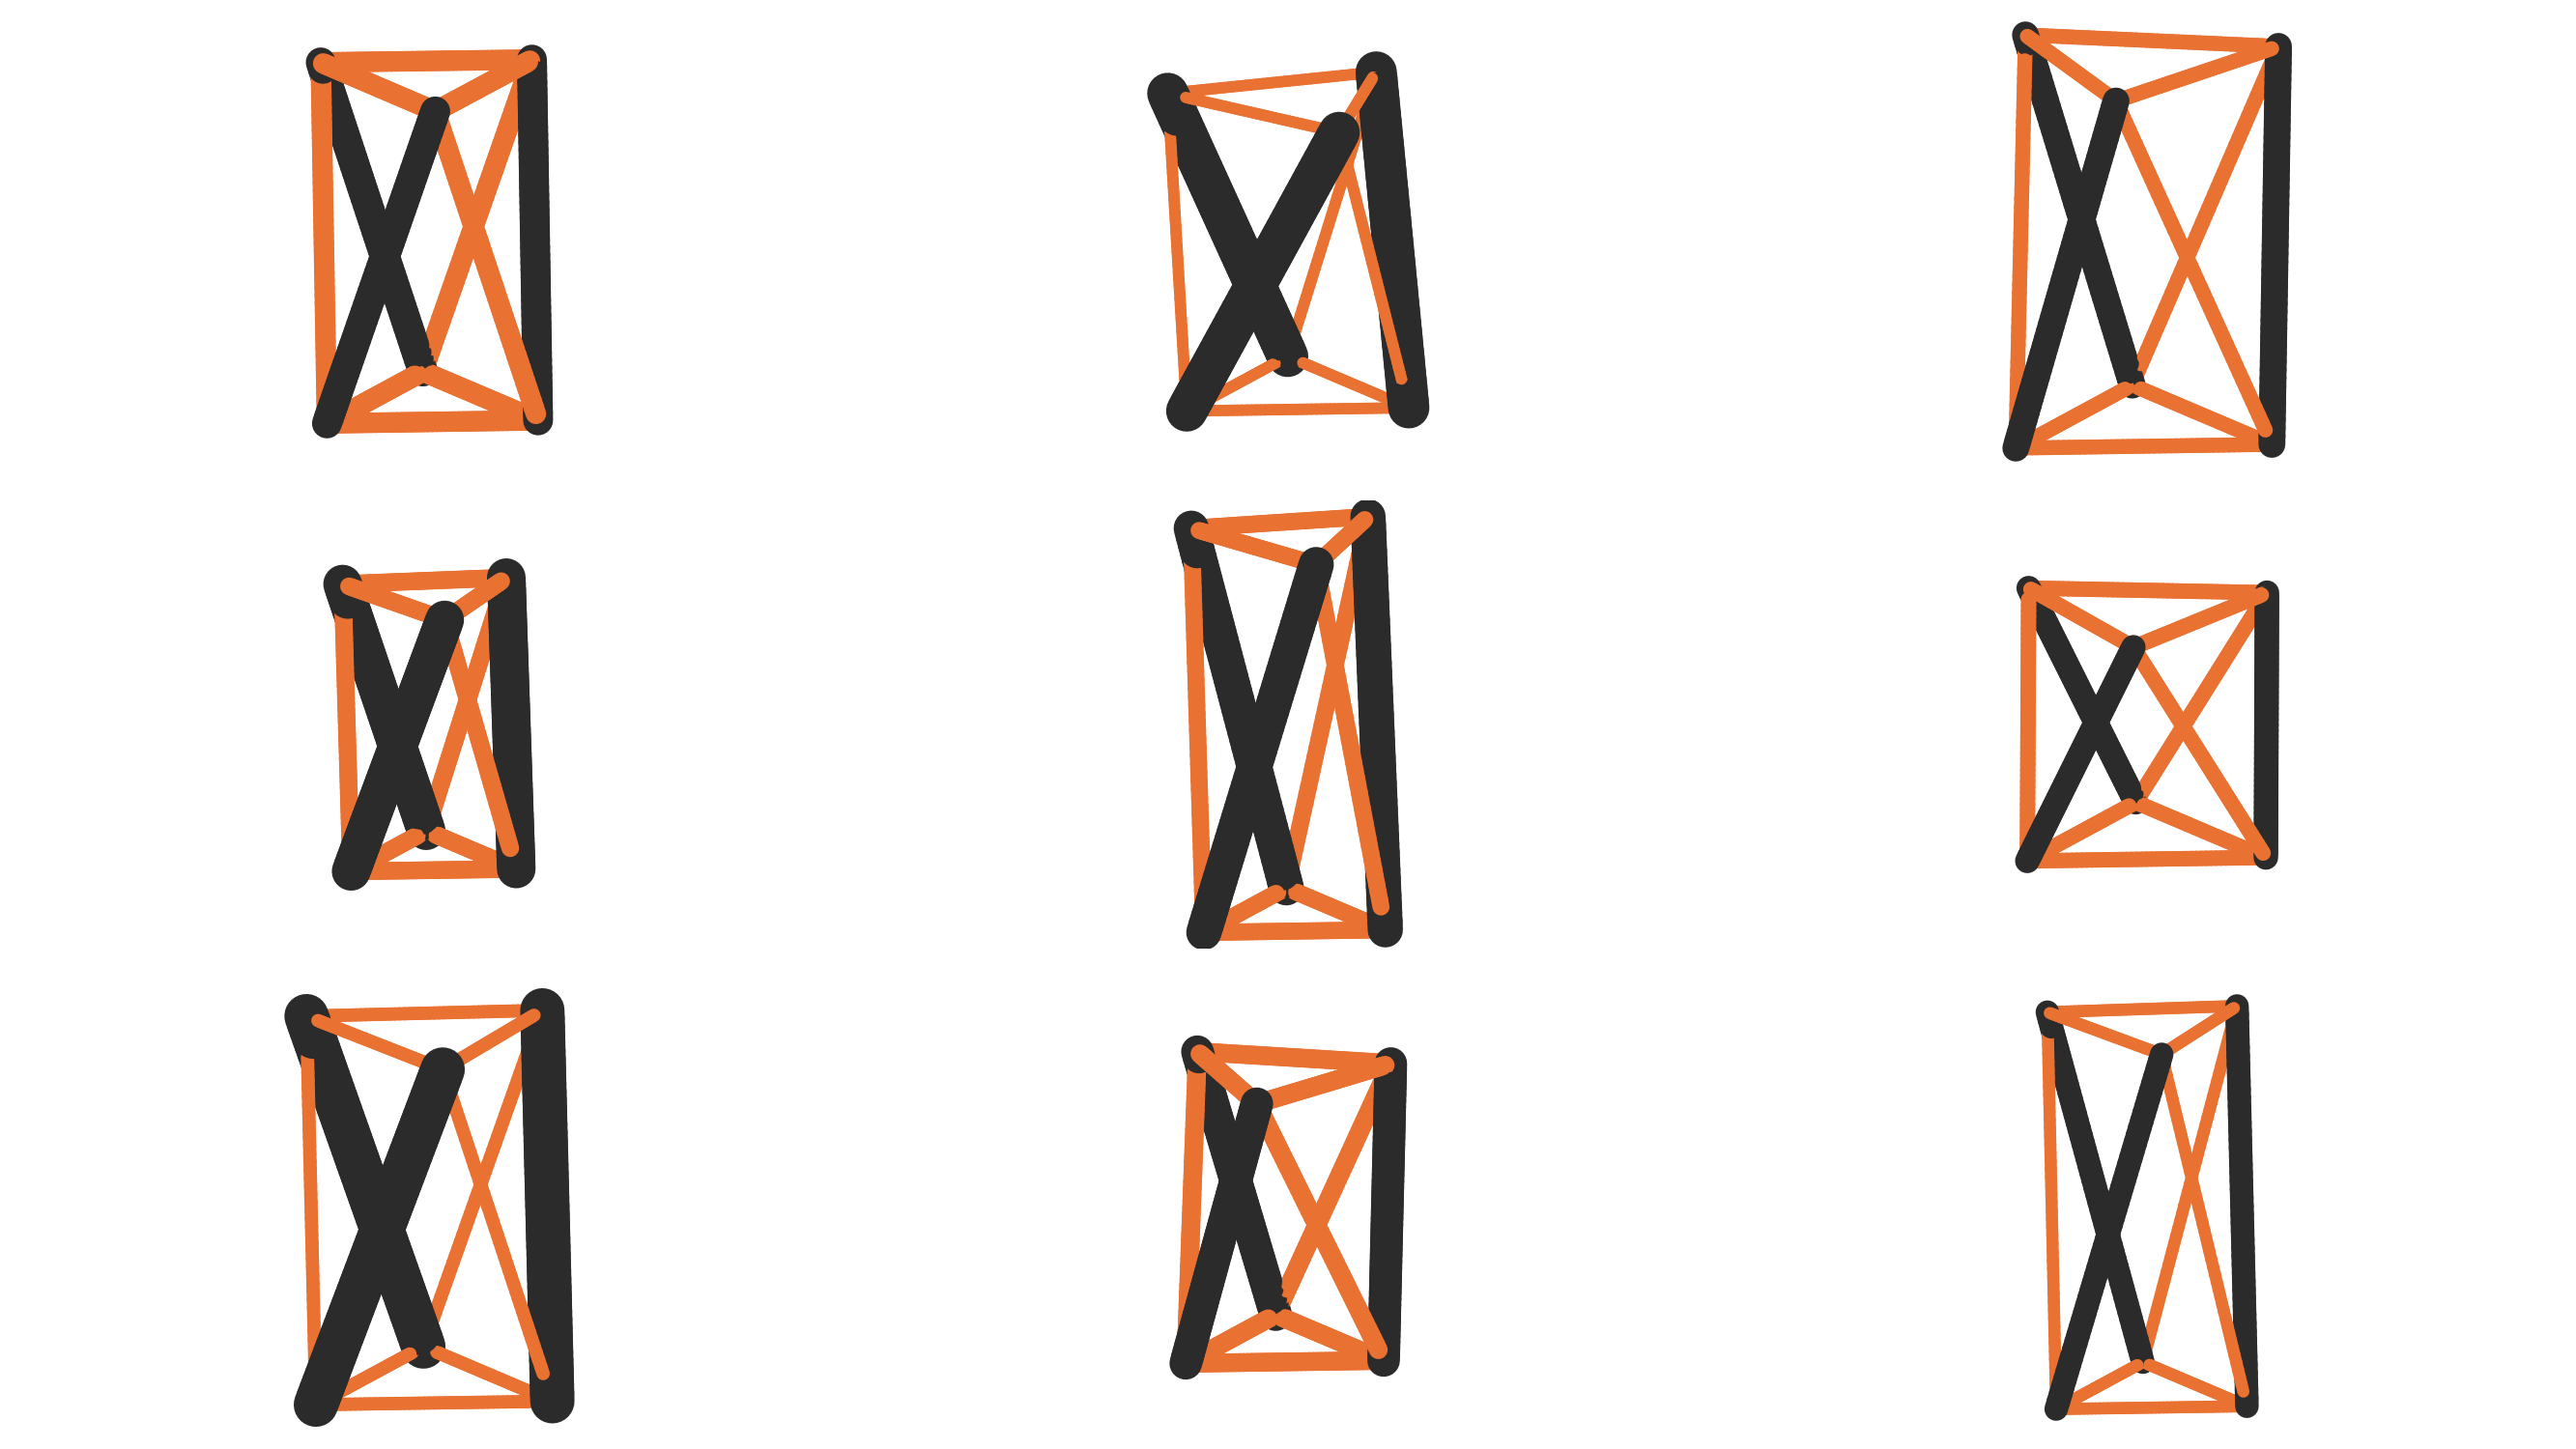
\includegraphics[width=\linewidth]{../figures/bo/fig-seed-designs.png}
  \caption{The nine seed geometries rendered to a common millimeter
    scale (rigid PLA struts in black, TPU tendons in orange). Every
    rendering corresponds to a physically printed article in the seed
    campaign.}
  \label{fig:seed-designs}
\end{figure}

\begin{table*}[t]
  \centering
  \caption{Seed-batch drop-tower results: 101 stabilized captures per
    article (103 for autv5r) at \SI{60}{in} onto the standardized
    polyurethane surface, CFC-180 filtering, counted after the first
    two warm-up drops of each session were discarded. Means $\pm$ one
    standard deviation over the stabilized drops; rows are ordered by
    $t_{180}$. $E_{\mathrm{reb}}$ uses each
    article's weighed mass per Eq.~\eqref{eq:objectives}. The ringdown
    frequency $f_n$ is a print-health descriptor, not an objective.
    A dash denotes a quantity that cannot be computed from the
    available record: article \textit{amdjwm} lacks a weighed mass and
    a confirmed design mapping (it is excluded from the surrogate fit
    and from all mass-dependent quantities), and no accepted $f_n$
    estimate is available for \textit{bag26v} or \textit{ajhby6}.
    Specs 03 and 06 were printed but have no drop sessions in the
    campaign record.}
  \label{tab:seed-results}
  \small
  \begin{tabular}{@{}llS[table-format=2.2]S[table-format=1.4]@{\,$\pm$\,}S[table-format=1.4]S[table-format=2.1]S[table-format=3.0]@{}}
    \toprule
    Design & Article & {Mass (g)} & \multicolumn{2}{c}{$t_{180}$} &
    {$E_{\mathrm{reb}}$ (mJ)} & {$f_n$ (Hz)} \\
    \midrule
    Spec 01 & 6lhxfy & 18.50 & 0.8931 & 0.0042 & 13.9 & 368 \\
    (unmapped) & amdjwm & {-} & 0.9805 & 0.0025 & {-} & 455 \\
    Spec 05 & 6nheas & 21.73 & 0.9970 & 0.0032 & 13.1 & 322 \\
    S0 ref. & bpx68c & 20.23 & 1.0111 & 0.0024 & 6.2 & 468 \\
    Spec 07 & ajhby6 & 20.53 & 1.0127 & 0.0038 & 6.1 & {-} \\
    Spec 00 & 9hhbkp & 21.62 & 1.0183 & 0.0017 & 6.9 & 364 \\
    Spec 04 & nvxsrv & 20.66 & 1.0275 & 0.0044 & 8.2 & 294 \\
    Spec 02 & autv5r & 22.04 & 1.0404 & 0.0035 & 8.8 & 386 \\
    Spec 08 & bag26v & 21.42 & 1.0616 & 0.0051 & 7.7 & {-} \\
    \bottomrule
  \end{tabular}
\end{table*}

\subsection{Model-Recommended Batches and Replication}
\label{sec:results:batches}

Table~\ref{tab:batch-results} reports the stabilized objectives for
the three model-recommended batches, and
Fig.~\ref{fig:front-evolution} overlays every measured article with
the non-dominated front after each batch (Pareto membership is
evaluated over articles with both objectives; the unmapped seed
article amdjwm is omitted because its missing weighed mass prevents
computing $E_{\mathrm{reb}}$). Dominated hypervolume, evaluated at
the fixed reference point $(t_{180}, E_{\mathrm{reb}}) =
(1.35, \SI{15}{mJ})$, grew from 3.155 after the seed batch to 3.969
after batch 2 ($+25.8\%$), 4.007 after batch 3 ($+0.9\%$), and 5.195
after batch 4 ($+29.7\%$): a 65\% total gain over the seed front. No
budget-matched quasi-random physical baseline has been run, so the
comparison the data support is against the campaign's own Sobol
seed: after batch 4, every member of the combined front (corny7,
corny6, drran5, drran3, r2d2c6) is a model-recommended design, and
the last seed article left the front when the batch-4 record
dominated it outright.

\paragraph{Batch 2 (Ax trials 10 to 18)} The first recommended batch
was generated from the seed fit and printed under the
constant-solid-mass projection, so its printed masses still spread
widely (17.91 to \SI{23.47}{g}; a regenerated constant-printed-mass
recommendation set is archived alongside the as-printed one, and the
two must not be conflated). The batch grew the front almost entirely
on the rebound axis: r2d2c6's \SI{4.1}{mJ} per drop is the lowest
rebound on record and still stands, and four batch-2 articles joined
the front. On the transmissibility axis the batch humbled its own
forecasts: the archived posterior predictions sat below the
measurements for nine of nine articles (mean absolute percentage
error 14.4\%; worst case r2d2c3, predicted 0.910, measured 1.334,
the strongest amplifier in the campaign record). That nine-of-nine
optimism widened the refit posterior for every batch that followed.

\paragraph{Batch 3 (Ax trials 28 to 36)} The first batch at constant
\emph{printed} mass (19.24 to \SI{20.06}{g}, CV 1.7\%) and the first
with the infill and filament axes active
(Section~\ref{sec:methods:parameterization}). It filled the knee of
the front rather than growing the box ($+0.9\%$ hypervolume; three
articles joined), and the recalibrated posterior held: eight of nine
articles measured within 0.3 posterior standard deviations of their
predictions (MAPE 3.8\%). The batch also delivered the campaign's
sharpest single surprise in both directions: the best-predicted
design (trial 32, predicted 1.020) measured 1.251, the strongest
amplification then on record, while the batch's only attenuator
(drran8, 0.980, drift-flagged, provisional) was its only twisted
design.

\paragraph{Batch 4 (Ax trials 37 to 45)} The acquisition split the
batch between the wide, high-twist, thin-cable family it had been
steering toward since batch 2 and a previously unvisited tall,
low-twist corner. The wide family delivered: four of nine articles
attenuate, and corny7, the batch's best-predicted design (trial 37,
predicted $0.934 \pm 0.13$), measured $t_{180} = 0.8031 \pm 0.0025$,
the strongest attenuation in the program, 10\% below the best seed
article and 21\% below the reference prism, at a mid-pack
\SI{9.4}{mJ} rebound; it dominates the seed attenuator on both
objectives (Fig.~\ref{fig:batch4-pred-vs-meas}). Within the
attenuating family the frozen predictions ranked the four
measurements perfectly (Spearman $\rho = +1.0$; $0.82$ across all
nine, where the five amplifier predictions span only 0.9\% and so
carry no ordering signal), batch MAPE was 6.0\%, and no article left
its predictive band by more than one standard deviation (the record
itself beat its band by 1.0 standard deviation in the good
direction). Per the between-seat replication rule, the batch-4
attenuation values, including the record, are single-seating
measurements whose re-seat confirmations are scheduled; one session
(corny5) carries a drift flag and its mean is provisional, and
another (corny6) was erratic (per-drop CV 2.0\%) but attenuates
under any reading of its record.

\paragraph{Replication: a second pass of batch 3} The batch-3 plate
was printed a second time (nine design replicates, the reprint
weighing \SI{0.27}{g} heavier article for article on average) and
the second set was drop-tested under the identical protocol, 360
drops across the two passes. Neither extreme of the first pass
recurred. Under \emph{any} pairing of the blinded session labels,
the design that measured 1.251 re-measured at most 1.090 (a drop of
at least 13\%) and the 0.980 attenuator re-measured at least 1.011,
so batch 3 contains no reproducibly attenuating design; under the
best-fit pairing, the same-design shifts have median $+1.2\%$, five
of nine fall inside the previously characterized $\pm 2.2\%$ re-seat
envelope, and the tails reach $-13.8\%$. The two passes cannot
separate seating effects from print-to-print differences, but the
methodological conclusion does not depend on that split: the 1.251
session had passed every within-session stability check (per-drop CV
0.77\%, no drift), so \emph{within-session stability does not
certify a measurement as a design property}. The between-seat
replication rule of Section~\ref{sec:methods:testing} was adopted in
response, the seed attenuator's 0.13\% agreement across an
independent re-seat shows that genuine attenuation does reproduce,
and a broadband seat gauge (the ratio of CFC-1000 to CFC-180
transmissibility; healthy sessions read 1.00 to 1.07) now
accompanies the rule as an advisory: every large same-design shift
observed so far carried a gauge reading of at least 1.15 in one of
its seatings, and all four batch-4 attenuators gauge healthy (0.98
to 1.06).

\begin{table*}[t]
  \centering
  \caption{Model-recommended batch results under the protocol and
    reporting conventions of Table~\ref{tab:seed-results} (CFC-180,
    stabilized means $\pm$ one standard deviation; about twenty
    drops per article against the seed batch's 101, with exact
    per-session counts in the archived per-drop records; rows
    ordered by $t_{180}$ within each batch).
    $E_{\mathrm{reb}}$ uses each article's weighed mass per
    Eq.~\eqref{eq:objectives}. ``Pred.'' is the posterior-mean
    $t_{180}$ archived when the batch was recommended, before any of
    its articles were tested. Batch-2 articles were projected to
    constant solid mass; batches 3 and 4 to constant printed mass
    (\SI{20.23}{g}). Flags follow the session record: $\dagger$
    marks a transmissibility-drift-flagged session whose mean is
    provisional, and $\ddagger$ marks the erratic corny6 session
    (per-drop CV 2.0\%).}
  \label{tab:batch-results}
  \small
  \begin{tabular}{@{}clcS[table-format=2.2]S[table-format=1.4]@{\,$\pm$\,}S[table-format=1.4]S[table-format=2.1]S[table-format=1.3]@{}}
    \toprule
    Batch & Article & Trial & {Mass (g)} & \multicolumn{2}{c}{$t_{180}$} &
    {$E_{\mathrm{reb}}$ (mJ)} & {Pred.\ $t_{180}$} \\
    \midrule
    2 & r2d2c7 & 15 & 18.51 & 0.9484 & 0.0008 & 12.2 & 0.905 \\
    2 & r2d2c1 & 13 & 19.38 & 0.9942 & 0.0021 & 6.0 & 0.948 \\
    2 & r2d2c2$^\dagger$ & 12 & 17.96 & 1.0411 & 0.0154 & 5.6 & 0.926 \\
    2 & r2d2c9 & 10 & 17.91 & 1.0530 & 0.0035 & 5.8 & 0.873 \\
    2 & r2d2c6 & 14 & 19.11 & 1.0548 & 0.0042 & 4.1 & 0.953 \\
    2 & r2d2c8 & 17 & 19.98 & 1.0704 & 0.0116 & 7.9 & 0.955 \\
    2 & r2d2c5 & 18 & 23.47 & 1.1516 & 0.0040 & 6.7 & 0.987 \\
    2 & r2d2c4 & 11 & 19.33 & 1.1847 & 0.0076 & 6.4 & 0.885 \\
    2 & r2d2c3 & 16 & 18.63 & 1.3337 & 0.0117 & 5.6 & 0.910 \\
    \midrule
    3 & drran8$^\dagger$ & 35 & 19.32 & 0.9804 & 0.0051 & 11.2 & 1.039 \\
    3 & drran1 & 36 & 19.31 & 1.0326 & 0.0016 & 18.1 & 1.051 \\
    3 & drran4 & 29 & 19.92 & 1.0344 & 0.0017 & 9.1 & 1.032 \\
    3 & drran2 & 33 & 19.33 & 1.0345 & 0.0006 & 11.8 & 1.056 \\
    3 & drran5 & 28 & 19.88 & 1.0373 & 0.0024 & 5.0 & 1.059 \\
    3 & drran3 & 31 & 19.92 & 1.0389 & 0.0012 & 4.2 & 1.043 \\
    3 & drran9 & 30 & 19.34 & 1.0425 & 0.0009 & 5.2 & 1.058 \\
    3 & drran6 & 34 & 19.24 & 1.0471 & 0.0040 & 4.8 & 1.065 \\
    3 & drran7 & 32 & 20.06 & 1.2513 & 0.0096 & 8.2 & 1.020 \\
    \midrule
    4 & corny7 & 37 & 19.62 & 0.8031 & 0.0025 & 9.4 & 0.934 \\
    4 & corny9 & 43 & 19.46 & 0.8766 & 0.0036 & 18.1 & 0.942 \\
    4 & corny6$^\ddagger$ & 41 & 19.45 & 0.9106 & 0.0181 & 5.7 & 0.943 \\
    4 & corny8 & 39 & 19.64 & 0.9535 & 0.0025 & 17.5 & 0.954 \\
    4 & corny1 & 42 & 20.20 & 1.0459 & 0.0029 & 8.7 & 1.010 \\
    4 & corny4 & 44 & 20.56 & 1.0475 & 0.0025 & 4.3 & 1.013 \\
    4 & corny3 & 45 & 20.15 & 1.0705 & 0.0013 & 8.8 & 1.004 \\
    4 & corny2 & 38 & 20.21 & 1.0846 & 0.0030 & 9.2 & 1.008 \\
    4 & corny5$^\dagger$ & 40 & 20.58 & 1.0876 & 0.0099 & 8.5 & 1.012 \\
    \bottomrule
  \end{tabular}
\end{table*}

\begin{figure*}[t]
  \centering
  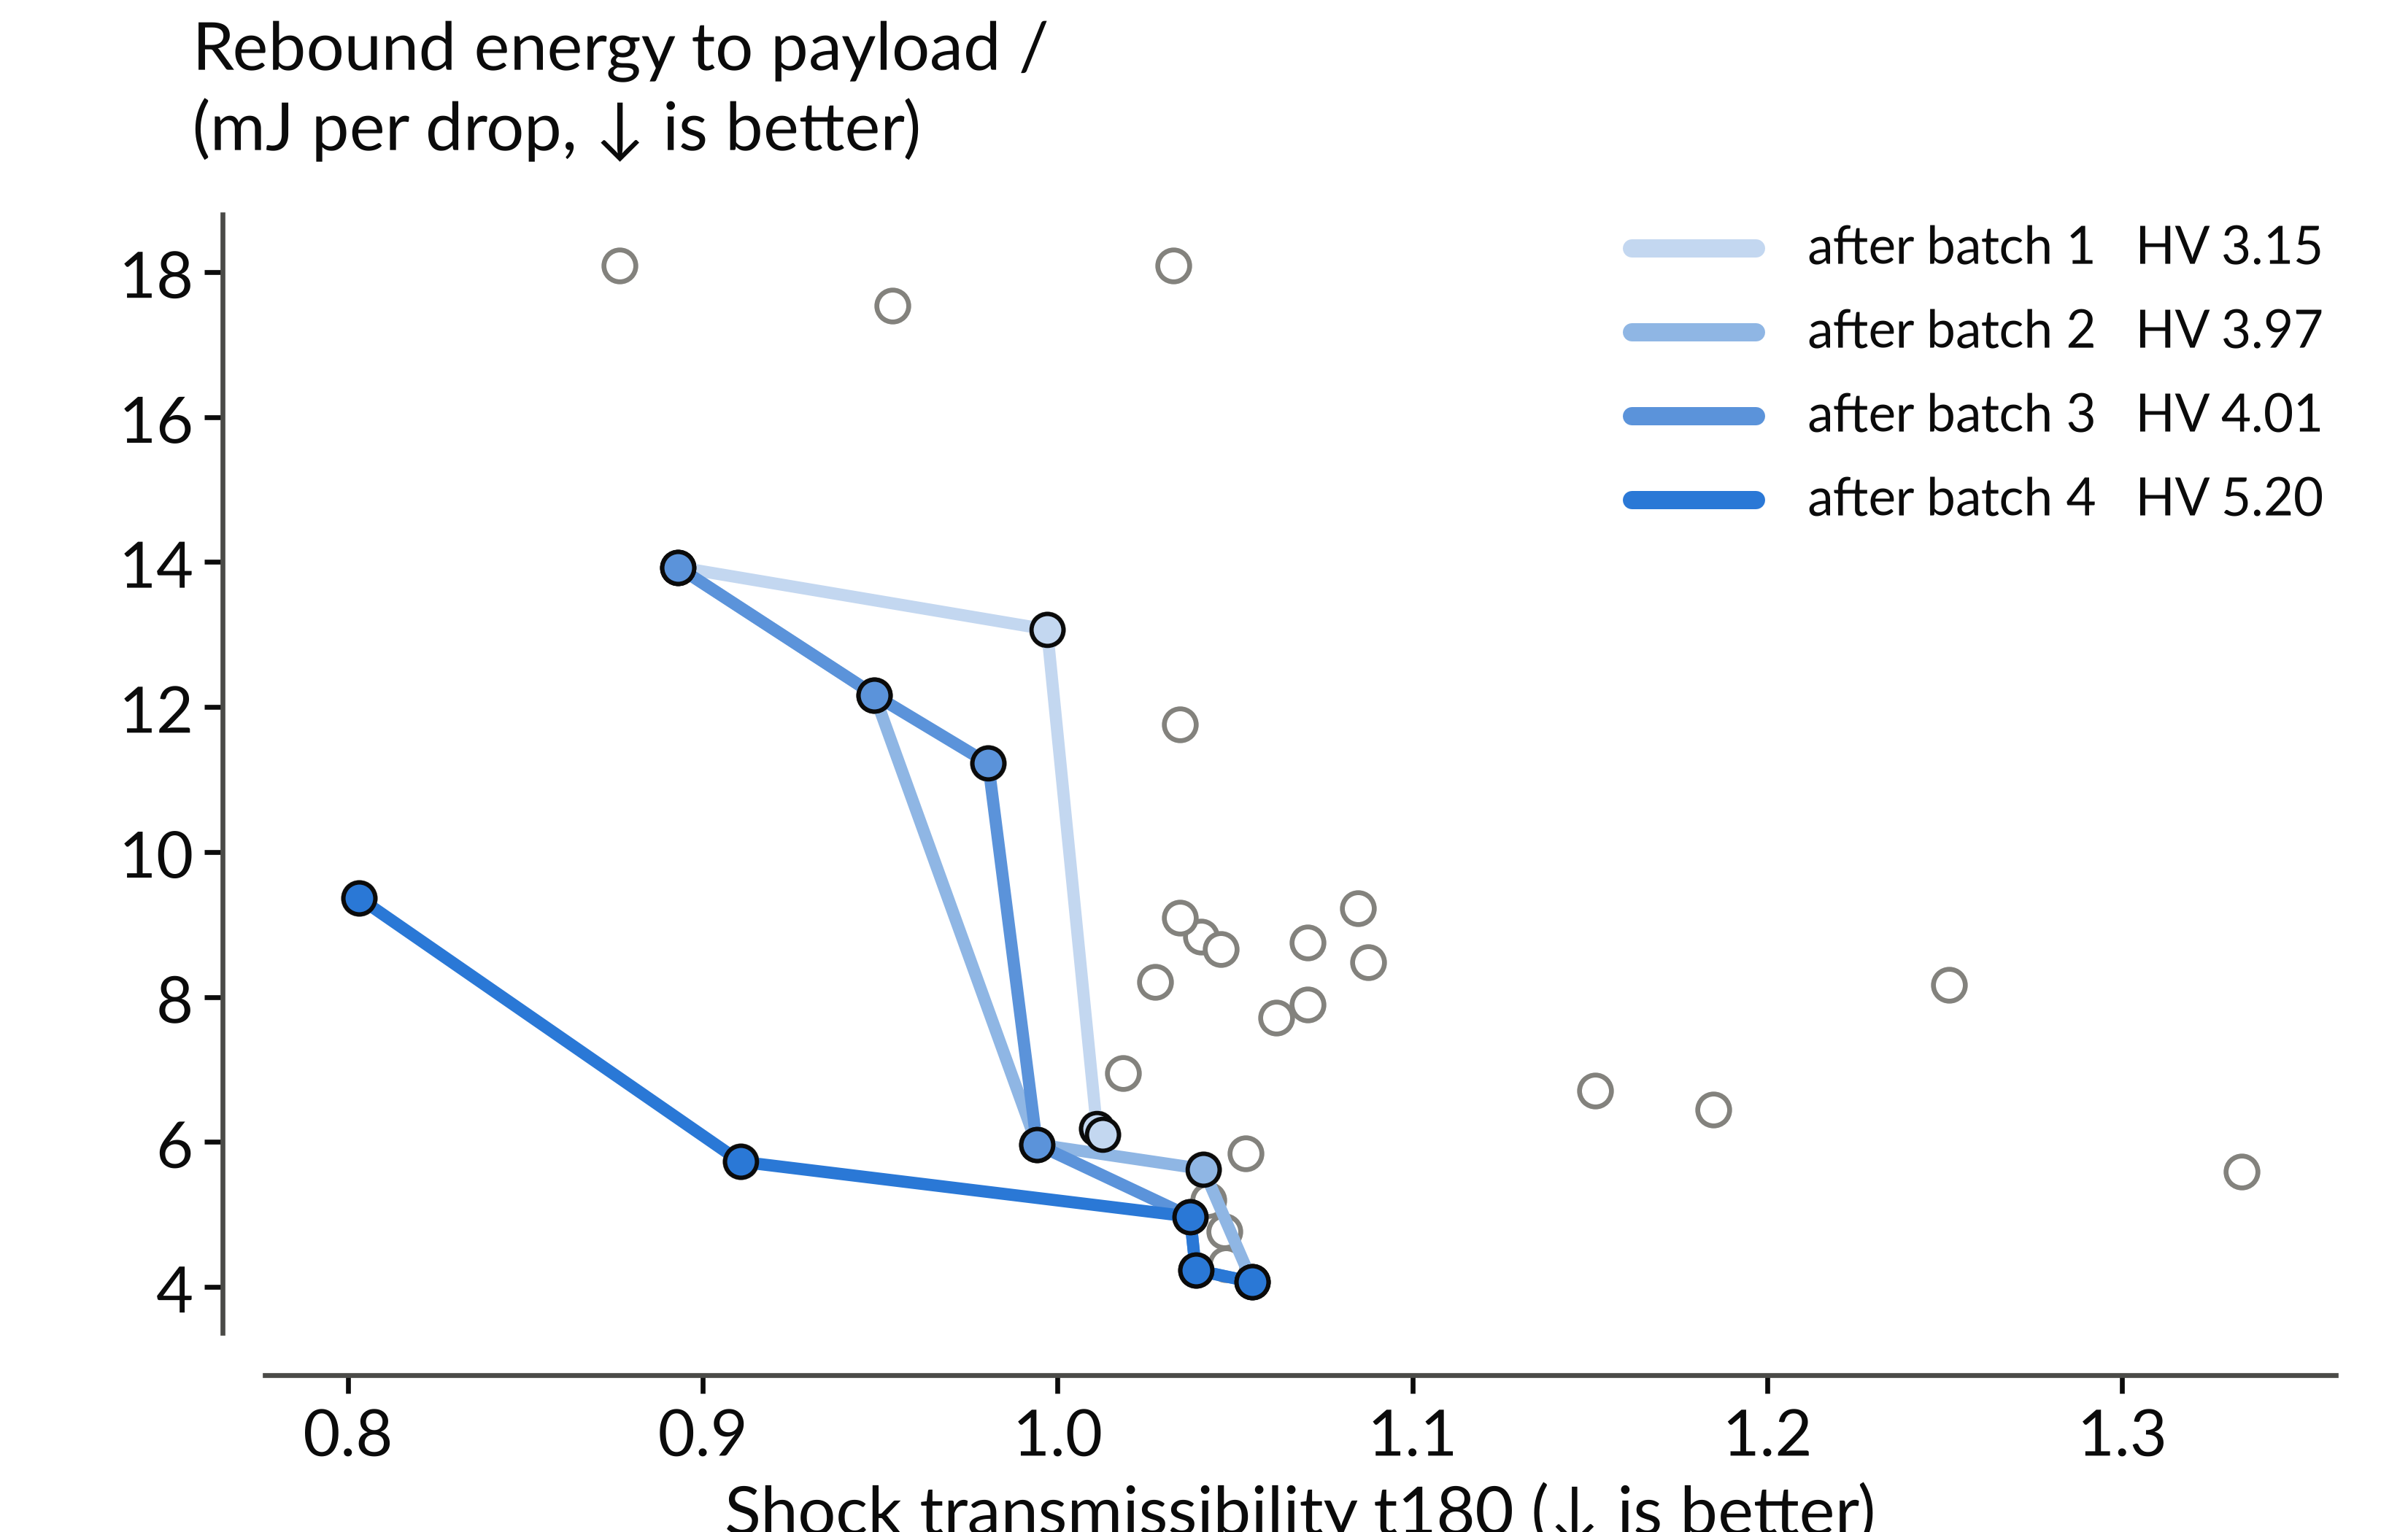
\includegraphics[width=0.85\textwidth]{../figures/bo/t3-prism-bo-front-evolution.png}
  \caption{Measured objective space and front evolution across the
    four batches. Gray circles are all measured articles at their
    stabilized means; the blue lines are the non-dominated fronts
    after each batch, with the dominated hypervolume at the
    $(1.35, \SI{15}{mJ})$ reference in the legend. Batch 2 grew the
    front on the rebound axis, batch 3 filled the knee, and batch 4
    broke the transmissibility floor. Both axes improve downward.}
  \label{fig:front-evolution}
\end{figure*}

\begin{figure*}[t]
  \centering
  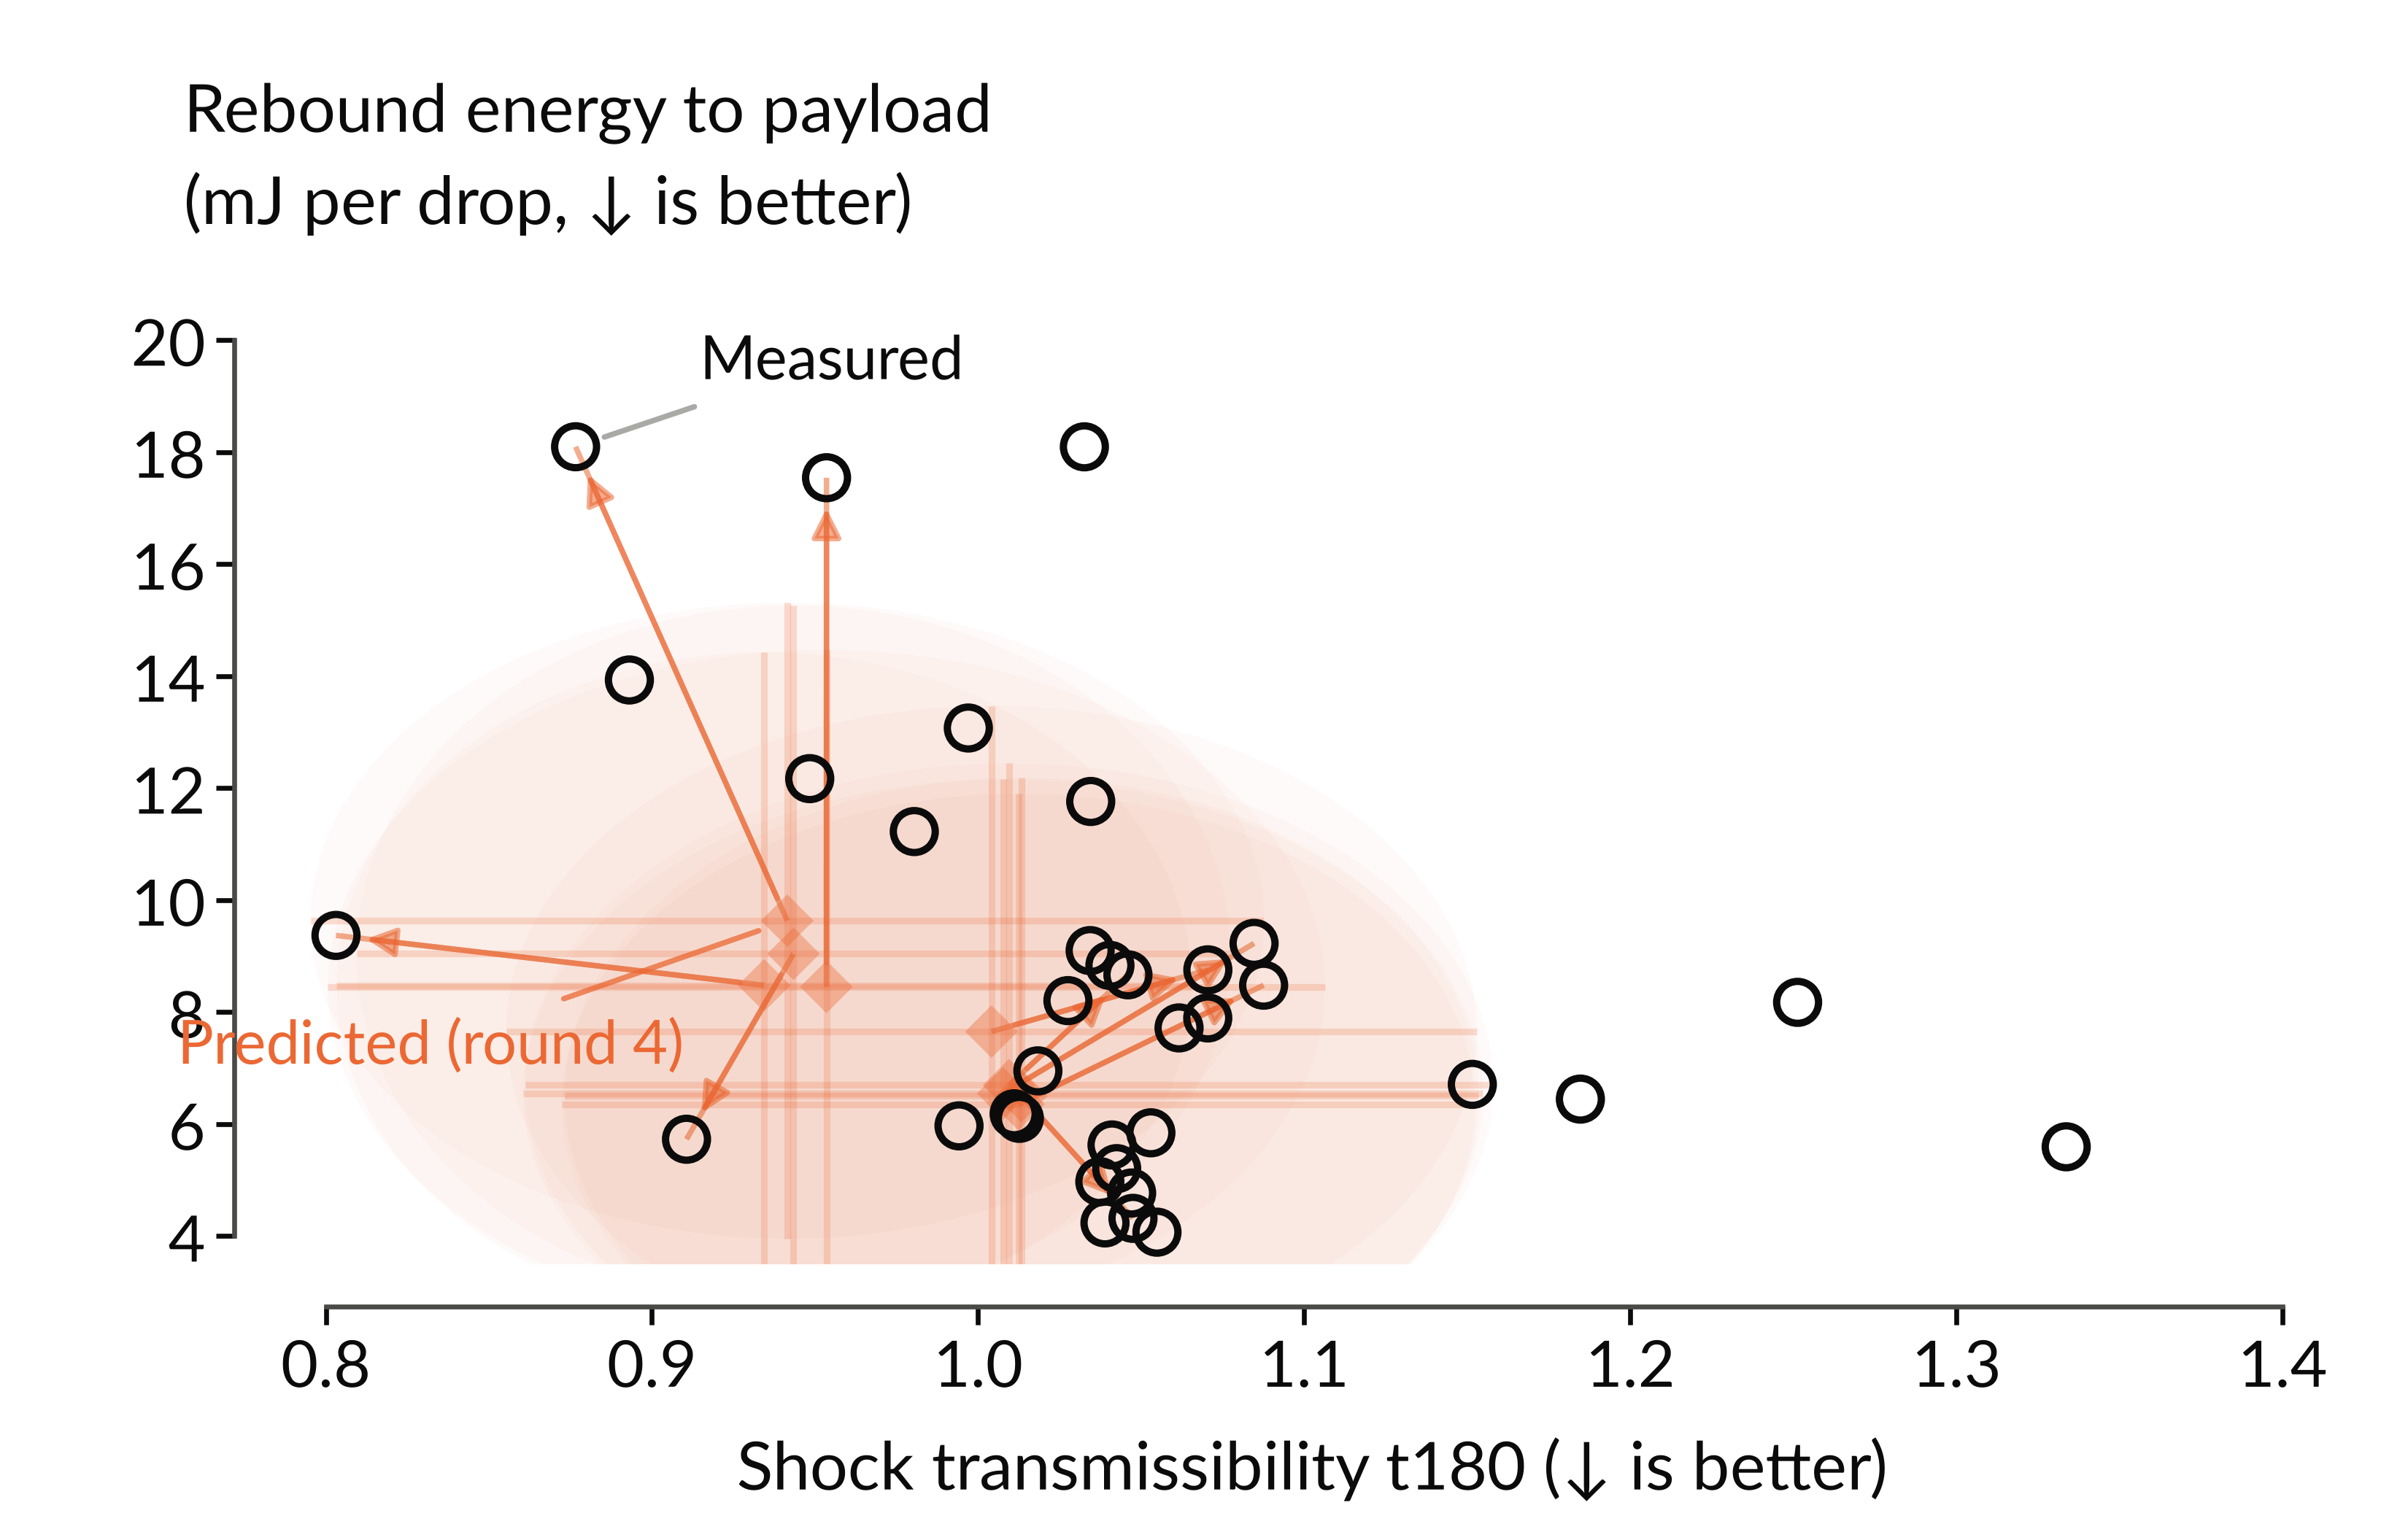
\includegraphics[width=0.85\textwidth]{../figures/bo/t3-prism-bo-round4-predicted-vs-actual.png}
  \caption{Batch-4 predictions against outcomes. Orange diamonds with
    bars are the archived posterior predictions (mean $\pm$ one
    standard deviation) for trials 37 to 45 at recommendation time;
    arrows connect each prediction to its article's measured value
    (black circles; all previously measured articles shown for
    context). The record attenuator corny7 (measured 0.803) is the
    left-most measured point. Both axes improve downward.}
  \label{fig:batch4-pred-vs-meas}
\end{figure*}

\subsection{Surrogate Audits Across the Campaign}
\label{sec:results:audits}

Each refit is audited with leave-one-out cross-validation (LOOCV;
one full NUTS refit per held-out article) and length-scale
diagnostics. Figure~\ref{fig:sensitivity} reports the seed-state
SAASBO feature importances (normalized inverse length scales, median
over the Monte Carlo draws with interquartile whiskers, over the five
design variables plus printed mass). At seven observations for six
correlated inputs these are prior-sensitive model diagnostics only:
no input separates decisively from the equal-share line, and none
supports a claim of variable relevance or ranking.

The honest headline of the cross-validation trajectory is that
held-out point accuracy \emph{declined} as the campaign grew:
$t_{180}$ LOOCV MAPE was 2.9\% with rank correlation $+0.76$ on the
seed state (8 articles, 6 model inputs), 5.4\% and $+0.60$ after
batch 2 (17 articles), and 6.2\% and $+0.19$ after batch 3 (26
articles, 12 inputs); the rebound channel reads 29.3\%, 23.6\%, and
32.2\% MAPE at the same states
(Fig.~\ref{fig:loocv}; the fold-level records are archived with the
campaign data). Three changes landed together and are confounded:
the input space doubled from 6 to 12 while the data grew only from
17 to 26, four of the six added axes carry a single value per batch
and are therefore perfectly confounded with batch, and batch 3
itself added the campaign's largest outliers. The held-out posterior
shrinks predictions toward the pooled mean, so the campaign's
defining extremes are exactly what it misses. The practical stance
this trajectory dictates, and the one the campaign took, is to treat
predicted columns as exploration bookkeeping rather than forecasts:
batch 4's value was the design family it selected and the record it
found, not its point accuracy, and its best-predicted article was
the record. Two further audit facts round out the picture. The
mass-transmissibility correlation fell from $r = 0.82$ over the
seed articles to $0.07$ over the 26 articles of batches 1 to 3, so
the constant-printed-mass projection removed the seed batch's
dominant confound. And the planned head-to-head calibration
comparison against a point-estimated single-task GP with the same
kernel has not yet been run, so no claim is made that SAASBO
outperforms it here.

\begin{figure}[t]
  \centering
  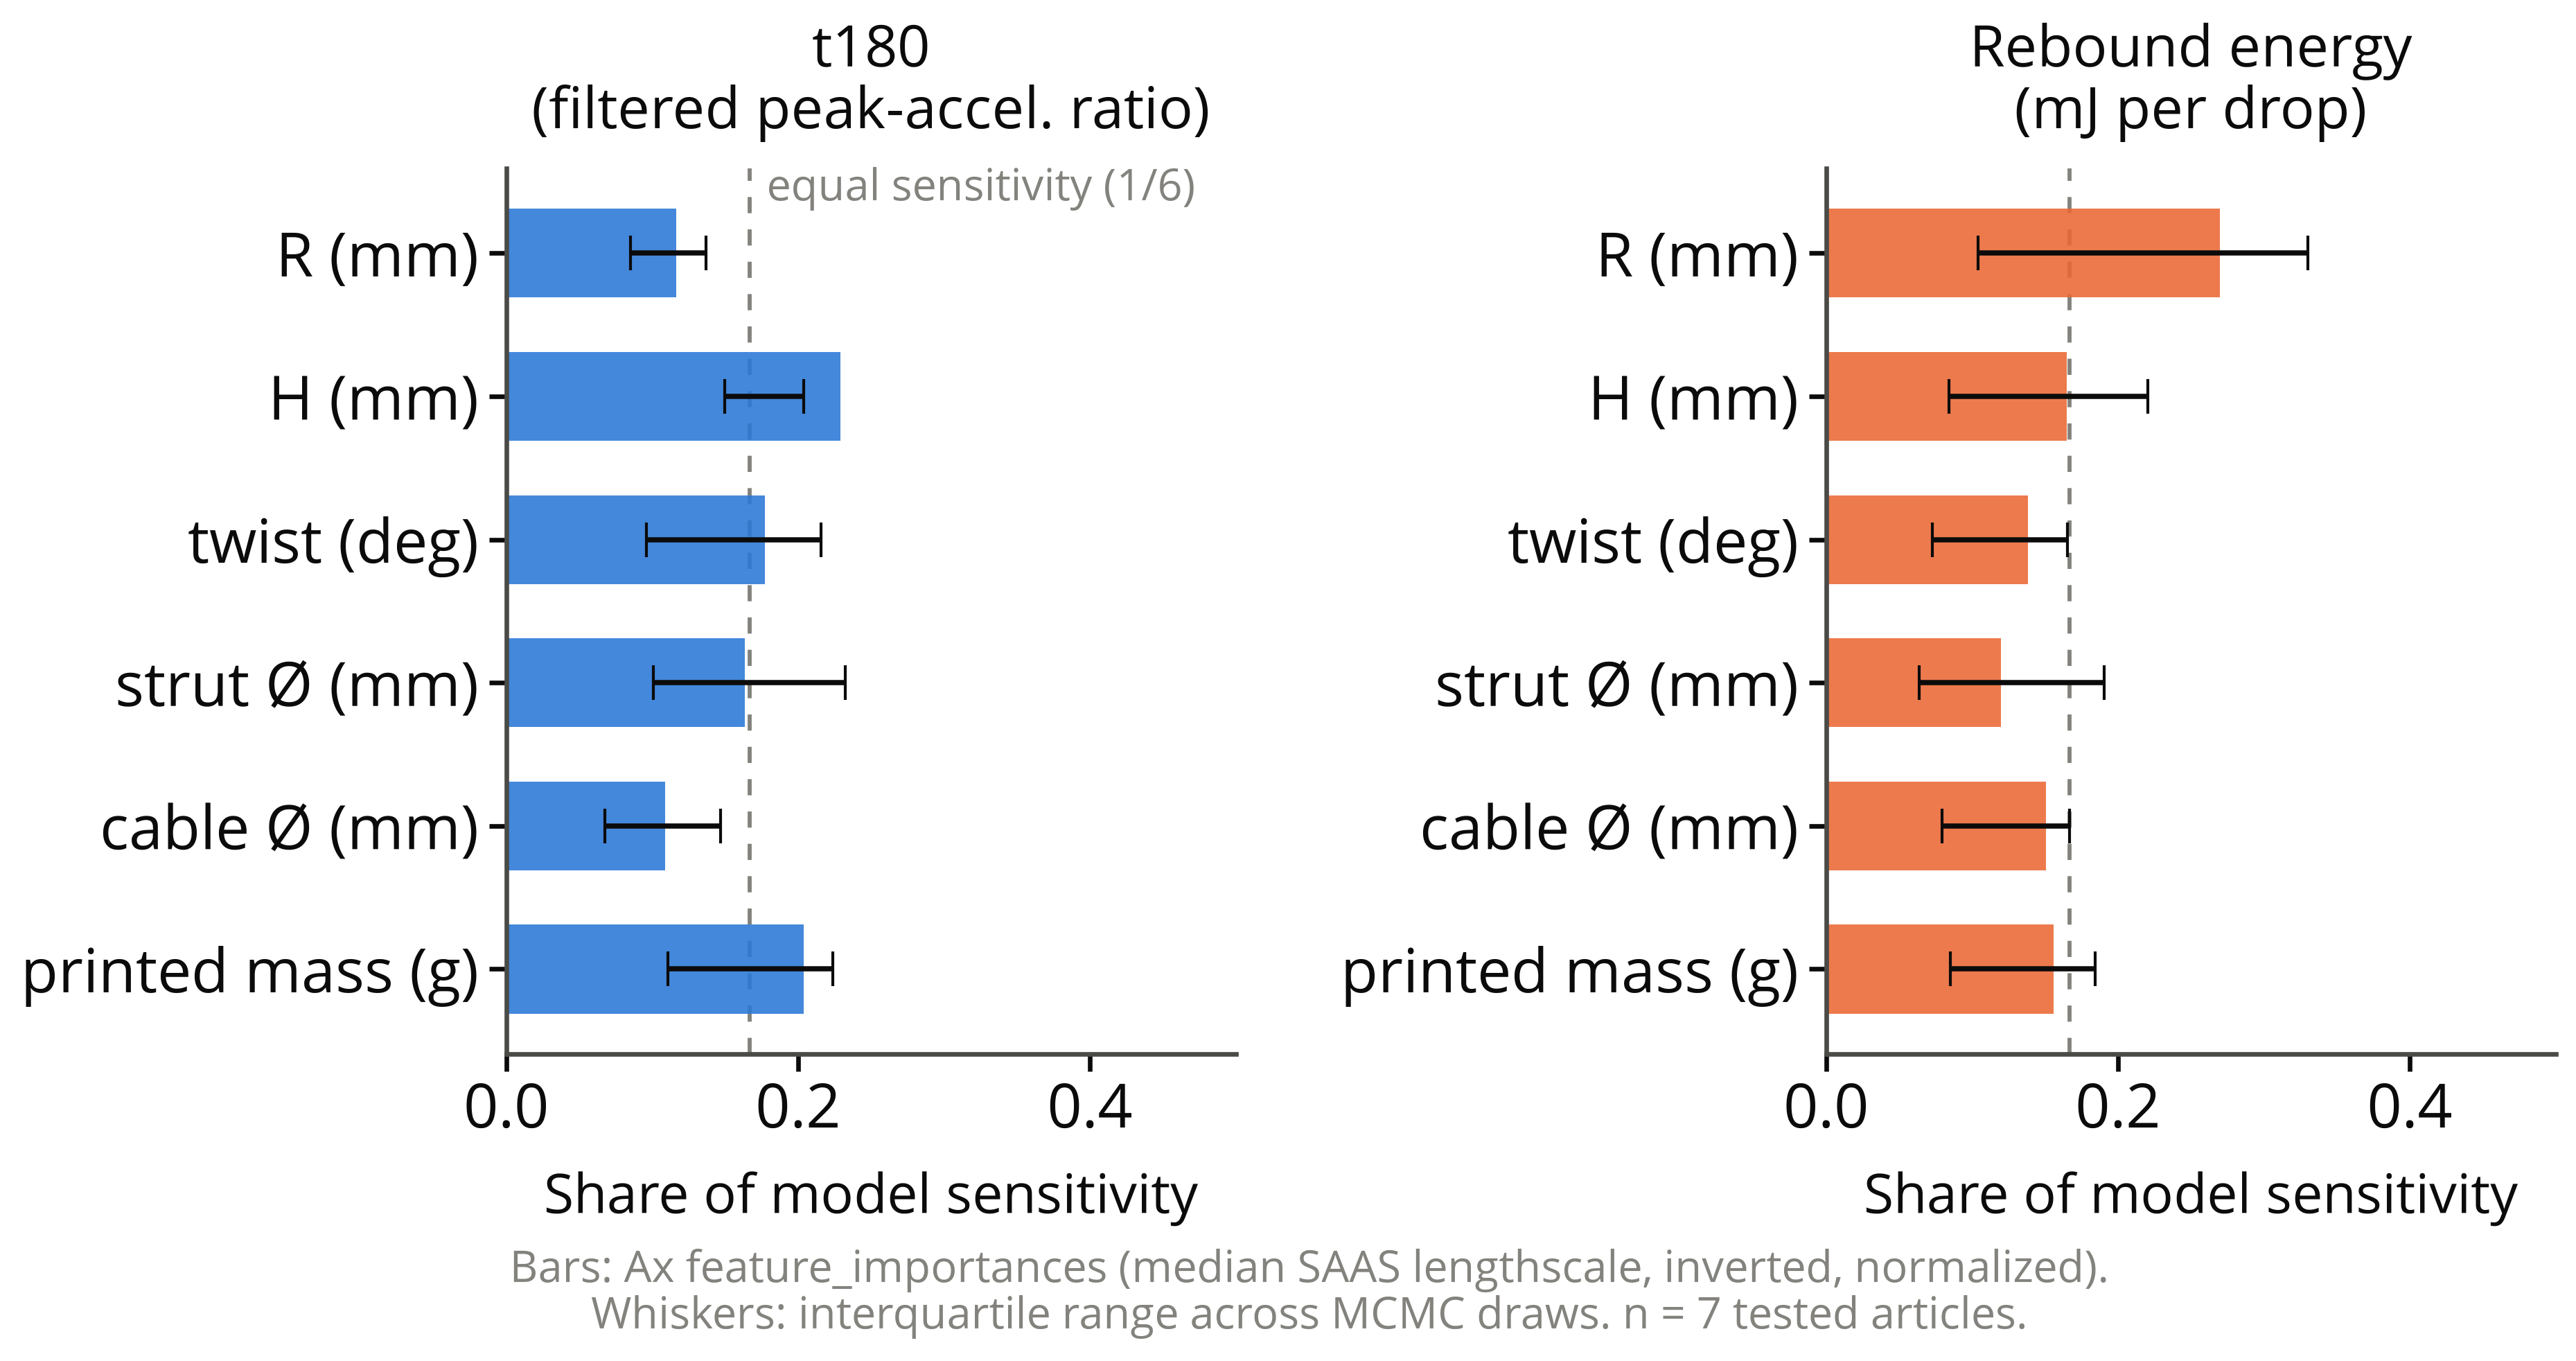
\includegraphics[width=0.92\linewidth]{../figures/bo/t3-prism-bo-round1-feature-importance.png}
  \caption{Seed-state SAASBO length-scale diagnostics per objective
    (normalized inverse length scales; median over MCMC draws,
    interquartile whiskers; inputs are the five design variables plus
    printed mass; the horizontal axis, labeled ``share of model
    sensitivity'' in the plot, is this normalized inverse-length-scale
    diagnostic). No input separates decisively from the equal-share
    line (dashed) at seven mapped articles, and these are
    prior-sensitive model diagnostics, not evidence of variable
    relevance.}
  \label{fig:sensitivity}
\end{figure}

\begin{figure}[t]
  \centering
  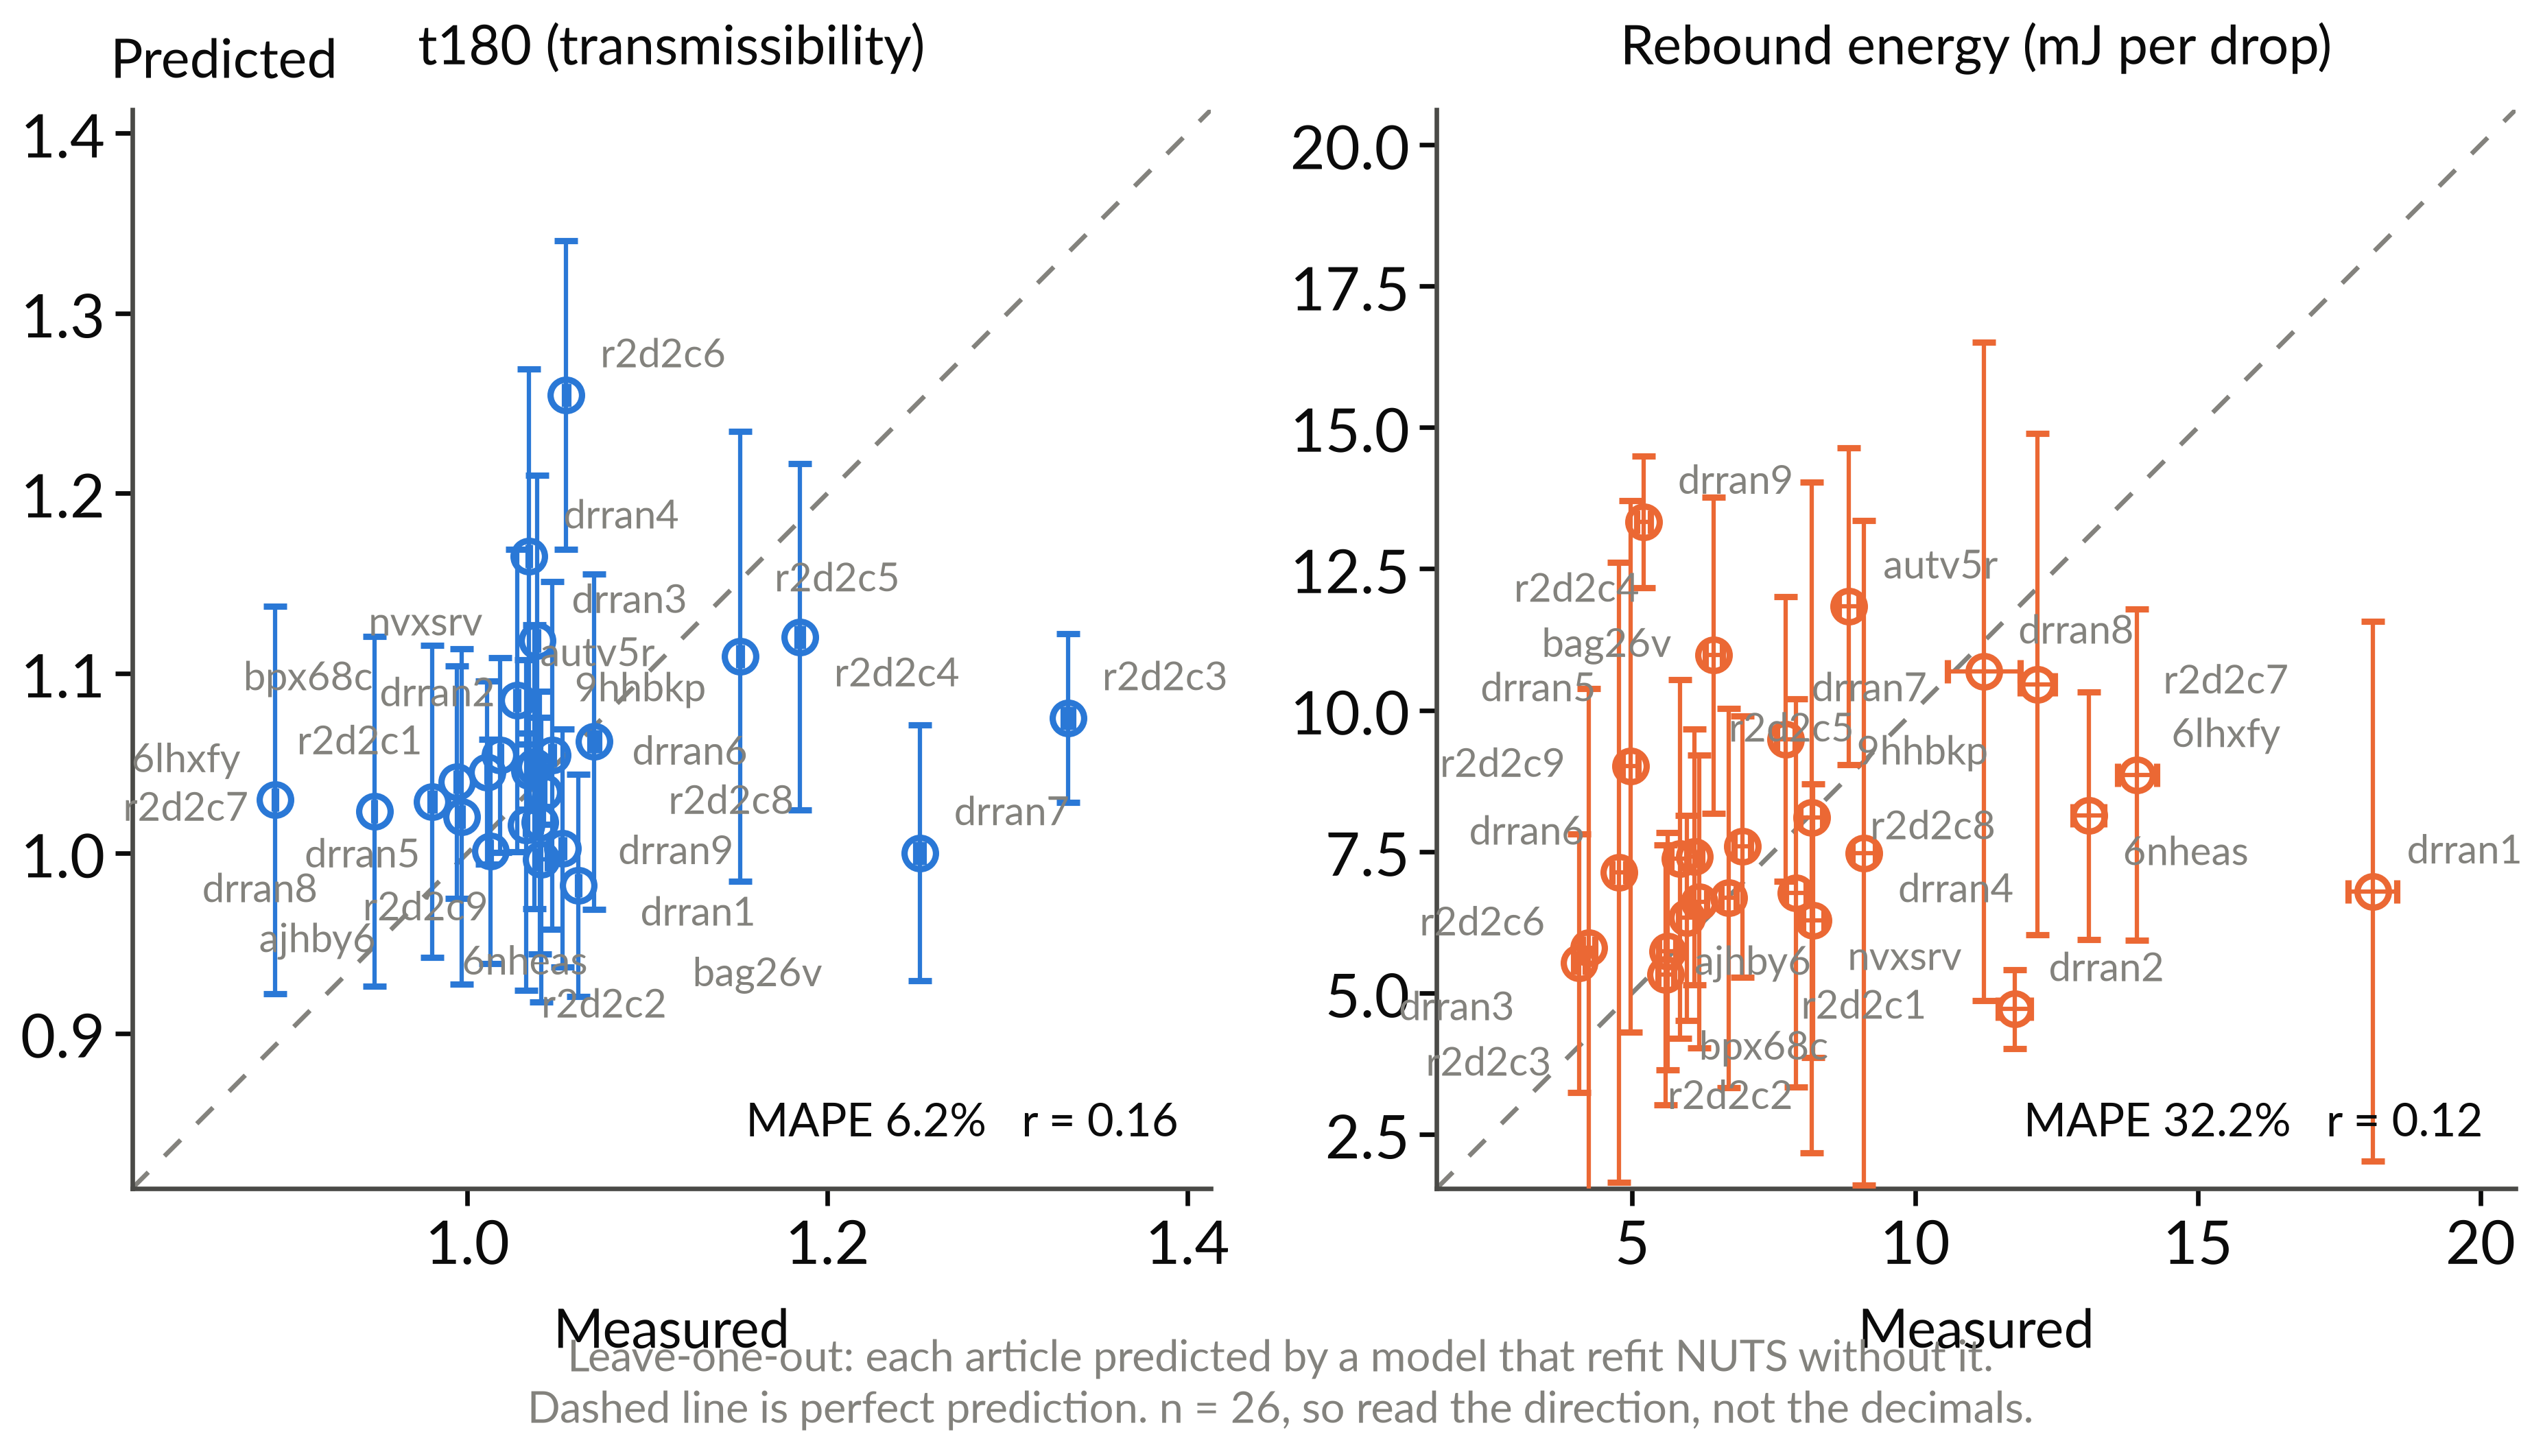
\includegraphics[width=0.92\linewidth]{../figures/bo/t3-prism-bo-round4-loocv.png}
  \caption{Leave-one-out cross-validation of the SAASBO surrogate on
    the 26 articles of batches 1 to 3 (one full NUTS refit per
    held-out article; 12 model inputs). Vertical bars are one
    posterior standard deviation of the held-out prediction;
    horizontal bars are the measured standard error as ingested. The
    dashed line is parity. The held-out posterior shrinks toward the
    pooled mean, so the extremes (r2d2c3, drran7, the seed
    attenuator) are the largest misses.}
  \label{fig:loocv}
\end{figure}

\paragraph{Studies pending} The re-seat confirmations of the batch-4
attenuators (the record article first), any batches beyond the
fourth (a fifth batch is generated and its print files staged, but
nothing from it appears here), the replicate rank-stability study of
Section~\ref{sec:methods:rankstability} (best-, mid-, and
worst-predicted in-sample designs re-printed in nominal triplicate),
the quasi-static crush campaign, and the metal-analog comparison
(Table~\ref{tab:metal-validation}) remain future work; none of their
values appear in this section.


% =============================================================================
\section{Discussion}
\label{sec:discussion}
% =============================================================================

\paragraph{What the campaign establishes} The four measured batches
settle four questions the planned-methods stage could only pose. The
end-to-end loop runs and closes, repeatedly: printed articles,
instrumented characterizations, a fitted fully Bayesian surrogate,
and three successive model-recommended batches whose own
measurements fed the next refit. The measurement distinguishes the
tested articles: the campaign $t_{180}$ means span 0.803 to 1.334,
far beyond within-session drop scatter, though
the batch-3 second pass shows that seating and print variation, not
drop scatter, set the resolution floor for any single article. The
physics is more adversarial than the cushioning intuition suggests:
at this scale and rate, most printed prisms \emph{amplify} the peak
shock reaching their top vertex (26 of 35 articles measured above
unity), which sharpened the campaign question from ``how much does
the architecture cushion'' to ``which corner of the design space
crosses into attenuation, and at what rebound cost.'' And the
batches answered that sharpened question, though not on the first
try: batch 2's forecasts were optimistic on nine of nine articles,
batch 3's best-predicted design was its worst amplifier, and batch 4
then delivered four attenuators from the wide, high-twist,
thin-cable family, led by its best-predicted design at
$t_{180} = 0.803$. The strongest attenuators still tend to carry
large rebound energies (the record article is mid-pack at
\SI{9.4}{mJ}, while the tall batch-4 family shows that near-unity
transmission with low rebound is reachable), so the front remains
genuinely two-dimensional.

\paragraph{Honest accounting of the objective stack} We
pre-registered an adversarial, data-first review of the objective
choices with an external AI referee that was required to commit to
its own objective set from the raw campaign files before reading
ours. Its findings temper the round-1 formulation and set the round-3
revision: the rebound fraction $e_{\mathrm{reb}}$ rests on a ballistic
interpretation of the second contact event that has not yet been
validated against synchronized video (a restrained-versus-unrestrained
check is scheduled); the apparent $t_{180}$-versus-rebound trade-off
is driven substantially by the single strongest attenuator (Spearman
$\rho = -0.39$, $p = 0.38$ across the reliable articles); and
per-drop standard errors are substantially smaller than the
between-article variation, and therefore understate design-level
uncertainty. The campaign's responses were physical rather than
statistical: the batch-3 plate was printed and tested twice, which
measured the same-design shift distribution directly (median
$+1.2\%$, heavy tails; Section~\ref{sec:results:batches}); the
between-seat replication rule now gates every extreme; rebound stays
a candidate constraint pending its ballistic validation; and the
constant-printed-mass projection removed the mass channel the review
flagged. We report this trajectory rather
than presenting the seed-state choices as final because the loop is
the contribution and revising objectives mid-campaign, with the
revision criteria stated in advance, is how such loops behave in
practice.

\paragraph{Mass as a confound and as a design variable} Holding
solid CAD mass constant did not hold printed grams constant: PLA
prints at partial infill while thin TPU cables print near solid, so
the seed articles span \SIrange{18.50}{22.29}{g}, and among the
mapped seed articles mass and $t_{180}$ are correlated
($r = 0.82$). Printed mass is itself induced by the geometry and is
strongly collinear with member dimensions (light articles \emph{are}
the thick-strut, thin-cable corner by construction), so the seed
observations cannot identify separate geometry and mass effects; a
post hoc mass-adjusted regression would be unstable and would
estimate a different, direct-effect quantity. The campaign's answer
was experimental design rather than adjustment: the calibrated
printed-mass model (Supplementary Information) let batches 3 and 4
compare geometries at fixed printed grams (batch mass CVs of 1.7 and
2.3\%), and the mass-transmissibility correlation across the
articles of batches 1 to 3 fell to $r = 0.07$. The confound was
broken by construction, and the mass-aware rebound objective keeps
grams penalized where they physically matter, in the energy returned
to the payload.

\paragraph{Relation to prior art, and why simulation sits outside
the loop} Relative to Pajunen
et~al.~\cite{pajunen2019design}, the present work varies the geometry
under an optimization loop rather than characterizing a single
fabrication condition; relative to Mo
et~al.~\cite{mo2023accelerated}, the loop's ground truth is physical
measurement, and no simulated number enters the objectives, the
acquisition, or candidate priority. That exclusion is a measured
decision, not an omission: an exploratory multi-engine simulation
study conducted alongside the campaign (rigid-body through
finite-element fidelities, archived in the project repository) could
not reproduce the amplification that dominates the measured record
(rigid-strut models cap the transmissibility near unity while most
printed articles exceed it), predicted design-invariant rebound
where the measurement discriminates strongly, and correlated only
weakly with the measured transmissibility. Its constant-mass
fairness constraints and its diagnosis of the seed batch's
mass-rebound confound did shape the campaign design, which is the
screening role we consider simulation to have earned here; anything
more must first demonstrate prospective predictive skill on
articles it has not seen. The measured near-unity
transmission of most seed articles also cautions against reading the
printed-tensegrity literature's attenuation results as generic: the
as-printed cells here are not pretensioned, and activating genuine
pretension in additively manufactured tensegrity (for example through
shrink-on-treatment routes) is an open direction we deliberately
scope out of the present campaign.

\paragraph{Practical considerations and path forward} TPU-PLA
interface durability under repeated impact remains open: no joint
failed during the repeated-drop measurement sessions (more than
1,400 stabilized captures across 35 articles plus the batch-3
second pass), but because
those sessions were not designed as controlled fatigue tests, the
observation does not establish interface durability, and pull-out
and fatigue characterization of the internal-anchor joint is an area
of planned follow-on work. Sensitivity to
print-process covariates (the print key logs defects, humidity, and
the mid-batch nozzle change for exactly this purpose) and transfer to
other material pairs likewise remain open. In the future we plan
the re-seat confirmations of the batch-4 attenuators, the replicate
rank-stability study of Section~\ref{sec:methods:rankstability}, the
metal-analog rank-transfer comparison of
Section~\ref{sec:methods:validation}, quasi-static testing as an
extension of the characterization
(Section~\ref{sec:methods:testing}), pretension activation, tiled
multi-cell absorbers and lattices~\citep{sabounizawadzka2024experimental},
and miniaturization to crutch-tip envelopes: long-term crutch use is
associated with substantial upper-extremity overuse injury and
ground-reaction-force impulses~\citep{requejo2005upperextremitykinetics,
rasouli2020walkingassistanceusing, manocha2021injuriesassociatedwith,
brasilbarrosdasilva2022painmappingand,
dozono2015peripheralneuropathiesin}; existing
spring-loaded~\citep{segura2007mechanicsofambulation,
zhang2011biomechanicalevaluationof} and
polymer-damped~\citep{macgillivray2016theinfluenceof} tip designs
reduce loading rate but not peak transmitted force, and recent
tensegrity crutch concepts~\citep{gu2026tensegritycrutches} and
open-source 3D-printed crutch
work~\citep{mottaghi2025opensource3dprintable} suggest a plausible
translation path, with adjacent footwear and orthotic lattice
studies~\citep{wang2025porouslatticestructure,
zhang2024pressurereducingdesignof,
janarthanan2024additivemanufacturingof} providing transferable design
heuristics.

\paragraph{Limitations} The measured evidence base is 35 articles
across four batches, but with one mechanical-response article per
design in the fit: only batch 3 has a second printed-and-tested set,
and that replication is what exposed the seating and print
sensitivity, so every single-article extreme, including the batch-4
record, is provisional until its re-seat. The drop protocol probes
one height, one impact surface, and axial loading only; the
specimens never leave the elastic regime, so crush-energy metrics
await the quasi-static campaign; per-specimen energy absorption in
joules is not recoverable from the current rig (the falling-mass and
displacement channels required for a force integral are not
instrumented); the four filament axes carry one value per batch and
are unidentified; the held-out prediction skill of the surrogate
declined as the input space grew
(Section~\ref{sec:results:audits}); one tested seed article lacks a
design mapping, one seed design's official article assignment
carries a recorded discrepancy, and two seed designs have no session
record; and all results are from a single printer, material pair,
and cell topology. The replication rule, the planned re-seat
confirmations, the replicate rank-stability study
(Section~\ref{sec:methods:rankstability}), and the metal-analog
protocol (Section~\ref{sec:methods:validation}) are the designed
responses to these limits.

% =============================================================================
\section{Conclusions}
\label{sec:conclusions}
% =============================================================================

We have presented an experiment-driven Bayesian-optimization
framework for designing multi-material 3D-printed tensegrity-inspired
energy absorbers, with TPU used in place of the traditional tension
elements and PLA members carrying compression most of the time, and
we have run it through the recommend, fabricate, measure, and update
cycle three times on physical hardware. The framework parameterizes a
$T_3$-prism family (five geometry variables, joined in batch 3 by
infill and filament process variables) under a constant-mass fairness
projection, fabricates each candidate in a single multi-material FDM
build with TPU tendons anchored inside the PLA strut ends,
characterizes every article with repeated instrumented drops (101
stabilized captures in the seed batch, about twenty thereafter), and
updates a fully Bayesian Gaussian-process
surrogate~\citep{balandat2020botorch, eriksson2021saasbo} that
recommends the next batch. Across the four measured batches (35
articles), the transmissibility spanned 0.803 to 1.334, most
articles amplified the peak shock, and the model-recommended batches
grew the dominated hypervolume 65\% over the Sobol seed front,
ending with a front whose five members are all model-chosen; the
batch-4 best-predicted design set the program record at
$t_{180} = 0.803$, ten percent below the best seed article, and
awaits its re-seat confirmation under the campaign's replication
rule. A second print-and-test pass of one batch showed that seating
and print variation, not drop-to-drop scatter, bound design-level
claims, which is the workflow lesson we consider most transferable.
The workflow is a candidate for other experimentally
evaluated architected structures whose constitutive response is
difficult to calibrate from first principles, but transfer beyond this
printer, material pair, topology, and axial impact condition remains
untested.

% =============================================================================
% Back matter
% =============================================================================
\section*{Acknowledgment} % ASME requests this exact spelling, singular.

This work was supported by the Brigham Young University Mentored
Research Grant program. The authors thank the undergraduate researchers
who carried out the multi-material printing and impact testing, and the
graduate co-mentor who supported day-to-day operations.
\todo{Confirm exact grant numbers and acknowledge any
NASA/Utah-Space-Grant-Consortium support per
acknowledgment-text guidelines.}

\section*{Funding Data}
\begin{itemize}
  \item Brigham Young University Mentored Research Grant.
\end{itemize}
\todo[inline]{Insert the MRG award number, and add the Utah NASA Space
Grant Consortium award if applicable.}

\section*{Conflict of Interest}
The authors declare no conflict of interest.

% Print the list of pending TODOs at the end -- the [disable] option
% on todonotes hides this automatically in the clean wrapper.
\listoftodos[Pending TODOs and figure/table placeholders]

% -----------------------------------------------------------------------------
% References (ASME numeric style; uses asmejour.bst)
% -----------------------------------------------------------------------------
\bibliographystyle{asmejour}
\bibliography{references}

\end{document}
:
%   \def\TODOOPTS{disable}    % manuscript.tex
%   \def\TODOOPTS{}           % manuscript-todos.tex
% =============================================================================

% PDF/A metadata (added in 2022; required by current asmejour for accessibility)
\DocumentMetadata{%
  lang        = en-US,
  pdfstandard = A-3u,
  pdfversion  = 1.7,
}

% Class options (see asmejour-template.pdf for the full list):
%   * lineno       -- numbered lines for review markup (run pdflatex twice)
%   * singlecolumn -- one-column draft layout (drop for ASME two-column final)
%   * nocopyright  -- suppress ASME copyright footer until acceptance
%   * upint, varvw -- typographic preferences carried over from the template
%   * hyphenate    -- allow hyphenation in typewriter font
\documentclass[lineno,nocopyright,upint,varvw,hyphenate]{asmejour}

\allowdisplaybreaks % from amsmath; multiline equations may break across pages

% --- Additional packages ---
% asmejour already loads: graphicx, hyperref, natbib, amsmath, amssymb,
% xcolor, booktabs, subcaption, caption, lineno, etc. Avoid re-loading those.
\usepackage{siunitx}
% House style: no en dashes anywhere, including ranges; siunitx ranges
% therefore render as "X to Y" rather than "X--Y".
\sisetup{range-phrase = { to }, range-units = single}
% tikz for measurement callouts overlaid on the printed-prototype photograph
% (Fig.~\ref{fig:printed-prototypes}); asmejour already loads graphicx/xcolor.
\usepackage{tikz}
\usetikzlibrary{arrows.meta}
% todonotes for in-margin TODO/figure-placeholder markers; toggled by the
% wrapper file (\TODOOPTS = "disable" hides everything; "" shows all).
\usepackage[\TODOOPTS,colorinlistoftodos,textsize=footnotesize]{todonotes}
\setlength{\marginparwidth}{2cm}

% Convenience macros that vanish along with todonotes when [disable] is set.
\newcommand{\figplaceholder}[3][]{%
  % #1 = optional [width]; #2 = label; #3 = caption / what to draw
  \begin{figure}[ht]
    \centering
    \fbox{\parbox[c][3.2cm][c]{0.85\linewidth}{\centering\textit{Figure
        placeholder: #3}}}%
    \caption{\textit{Placeholder.} #3}
    \label{fig:#2}
  \end{figure}%
  \todo[inline,color=orange!30]{Figure \texttt{#2}: #3}%
}

% Synthetic-placeholder (dummy) data convention. Any value that is a
% stand-in rather than a measurement is typeset in this violet color in
% BOTH wrappers (clean and todos) so no reader can mistake it for data.
% As of 2026-09-15 the Results carry no violet values: the former dummy
% round-2 numbers were replaced by the measured batch 2-4 record
% (manuscript/data/, snapshotted from the campaign branch at e25ebf5).
% The macro stays defined for future placeholders.
\definecolor{dummydata}{RGB}{142,68,173}
\newcommand{\dummy}[1]{\textcolor{dummydata}{#1}}

\newcommand{\tabplaceholder}[2]{%
  % #1 = label; #2 = caption / contents description
  \begin{table}[ht]
    \centering
    \caption{\textit{Placeholder.} #2}
    \label{tab:#1}
    \begin{tabular}{@{}lll@{}}
      \toprule
      Column A & Column B & Column C \\
      \midrule
      \multicolumn{3}{c}{\textit{(table contents pending)}} \\
      \bottomrule
    \end{tabular}
  \end{table}%
  \todo[inline,color=orange!30]{Table \texttt{#1}: #2}%
}

% --- PDF metadata ---
\hypersetup{%
  pdfauthor   = {Jeffrey R. Hill and Sterling G. Baird},
  pdftitle    = {Experiment-Driven Bayesian Optimization of the Impact Response
                 of Multi-Material 3D-Printed Tensegrity-Inspired Structures},
  pdfkeywords = {tensegrity, multi-material 3D printing, Bayesian optimization,
                 impact mitigation, design of experiments},
  pdfsubject  = {Manuscript draft for ASME Journal of Mechanical Design},
}

% --- Journal name (printed in the running head; omit "Journal of") ---
\JourName{Mechanical Design}

\begin{document}

% =============================================================================
% Author block(s) -- one \SetAuthorBlock per author (or per shared affiliation)
% Mark corresponding author(s) with \CorrespondingAuthor (no space before).
% =============================================================================
% Author order per @me-madsen review (PR #20): equal-contribution and
% corresponding-author scheme is \textsuperscript{*} = equal contribution,
% \textsuperscript{\dag} = also equal contribution, \textsuperscript{\ddag} =
% corresponding author (see legend \todo after \maketitle).
\SetAuthorBlock{Marcus E. Madsen\textsuperscript{*}}{%
  Department of Mechanical Engineering,\\
  Brigham Young University,\\
  Provo, UT 84602, USA
}

\SetAuthorBlock{Audrey K. Christiansen\textsuperscript{*}}{%
  Department of Mechanical Engineering,\\
  Brigham Young University,\\
  Provo, UT 84602, USA
}

\SetAuthorBlock{Jinkwan Han\textsuperscript{*}}{%
  Department of Mechanical Engineering,\\
  Brigham Young University,\\
  Provo, UT 84602, USA
}

\SetAuthorBlock{Jeffrey R. Hill\textsuperscript{\dag\ddag}\CorrespondingAuthor}{%
  Department of Mechanical Engineering,\\
  Brigham Young University,\\
  Provo, UT 84602, USA\\
  email: jeff.hill@byu.edu
}

\SetAuthorBlock{Sterling G. Baird\textsuperscript{\dag\ddag}\CorrespondingAuthor}{%
  Department of Mechanical Engineering,\\
  Brigham Young University,\\
  Provo, UT 84602, USA\\
  email: sterling.baird@byu.edu
}

\title{Experiment-Driven Bayesian Optimization of the Impact Response of
       Multi-Material 3D-Printed Tensegrity-Inspired Structures}

% Keywords are printed at the end of the abstract; must precede \end{abstract}.
\keywords{tensegrity, multi-material 3D printing, Bayesian optimization,
          impact mitigation, design of experiments}

% -----------------------------------------------------------------------------
% Abstract -- JMD requires 150--200 words, Latin characters only (no math),
% structured as background, approach, results, conclusions.
% -----------------------------------------------------------------------------
\begin{abstract}
Tensegrity-inspired rigid-soft architectures are candidates for impact
mitigation, but their transmitted-shock response is difficult to predict
from simulation alone. We report an experiment-driven Bayesian
optimization campaign over a co-printed polylactic-acid/thermoplastic-%
polyurethane three-strut prism family. The search space begins with five
continuous geometry variables and, from the third batch, adds
per-article infill densities and batch-level filament settings.
Candidate geometries are projected to a common mass budget and
fabricated in single multi-material builds, and each article is
characterized by repeated instrumented drops: 101 stabilized captures in
the seed batch and about twenty thereafter. The optimizer jointly
minimizes the filtered peak-acceleration ratio (transmissibility) and
the rebound energy returned to the payload. Most printed articles
amplify the peak shock, so the campaign question became which corner of
the design space attenuates. Across one Sobol seed batch and three
model-recommended batches, 35 articles in all, the dominated hypervolume
grew 65 percent, the final Pareto front is entirely model-chosen, and
the fourth batch's best-predicted design set the program record,
lowering transmissibility to 0.803, ten percent below the best seed
article. A second print-and-test pass of one batch showed that seating
and print variation, not drop-to-drop scatter, limit design-level
claims, motivating the replication rule we adopt.
\end{abstract}

\maketitle

\begin{center}
  \fcolorbox{dummydata}{dummydata!6}{\parbox{0.94\linewidth}{\small
  \textcolor{dummydata}{\textbf{Draft note (remove before submission):} this
  draft is written at the intended final scope of the study, and any value
  printed in this violet color is a synthetic placeholder rather than a
  measurement. As of 2026-09-15 the Results contain no violet values: all
  four reported batches (35 articles) are measured data from the committed
  campaign record. Still pending, and written as future work rather than
  as results: the re-seat confirmation of the batch-4 record article, any
  batches beyond the fourth, the replicate rank-stability study (best-,
  mid-, and worst-predicted in-sample designs in nominal triplicate), the
  quasi-static crush campaign, the metal-analog comparison, and the
  archival (Zenodo) code release.}}}
\end{center}

\todo[inline]{\textbf{Author order / contributions (per @me-madsen).} Planned
  order: Marcus E. Madsen\textsuperscript{*}, Audrey K.
  Christiansen\textsuperscript{*}, Jinkwan Han\textsuperscript{*}, Jeffrey R.
  Hill\textsuperscript{\dag\ddag}, Sterling G. Baird\textsuperscript{\dag\ddag},
  where \textsuperscript{*}~=~equal contribution, \textsuperscript{\dag}~=~also
  equal contribution, and \textsuperscript{\ddag}~=~corresponding author.
  Confirm affiliations and add emails for M.~Madsen, A.~Christiansen, and
  J.~Han, and typeset the equal-contribution footnote per ASME JMD style.}

% =============================================================================
% Body -- IMRaD structure per JMD submission instructions
% =============================================================================
\section{Introduction}
\label{sec:introduction}

Tensegrity structures are assemblies of rigid compression members
suspended within a continuous network of tension members; their defining
property, that no two rigid bars touch, yields lightweight assemblies with
remarkable strength-to-weight ratios and tunable nonlinear mechanical
responses~\citep{skelton2009tensegrity, sultan2009tensegrity}. These
properties have made tensegrity attractive across scales, from
metamaterial unit cells~\citep{amendola2014experimental,
zhang2018tensegrity, fraternali2015tensegrity} to compliant impact-absorbing
robots developed for planetary landing~\citep{agogino2018superball,
caluwaerts2014superball, sabelhaus2015system, vespignani2018design,
deitrich2022titan}. Recent work has shown that \emph{tensegrity-inspired}
unit cells can be directly 3D-printed and exhibit load-limiting plateaus
under drop-weight impact~\citep{pajunen2019design}, opening a path
toward additively manufactured architected absorbers. Throughout, we use
\emph{tensegrity-inspired} for printable cells that borrow the separated
compression-member and tension-network geometry of tensegrity while
relaxing defining mechanical conditions of classical tensegrity. In the
present specimens, the TPU tension elements are extensible, the PLA struts
may share printed junctions, and no pretension is activated or measured.
We therefore do not claim classical tensegrity, prestress-stabilized
behavior, or equivalence to an ideal cable-strut prism.

Multi-material fused-deposition modeling (FDM) that pairs a rigid polymer
such as polylactic acid (PLA) with a soft, rate-dependent elastomer such as
thermoplastic polyurethane (TPU) has been used to fabricate rigid-soft
architected energy absorbers on a single platform: thick-panel
origami metamaterials with PLA panels and TPU hinges~\citep{ye2023multimaterial}
and ABS/TPU honeycombs with tunable stiff/flexible
proportions~\citep{khatri2024energy}. The same rigid-soft co-printing
capability makes it possible to rapidly fabricate diverse tensegrity-inspired
geometries, which adopt a discrete-compression/continuous-tension topology
rather than an origami or honeycomb one. Although extruded TPU does not behave
as an idealized
inextensible cable, its rate-dependent damping is a desirable property
for impact-absorption applications and complements the elastic stiffness
of the PLA compression members rather than competing with it.

Designing such architected absorbers is fundamentally a
\emph{design-of-experiments} problem: the configuration space spanned by
strut geometry, tension-element cross-section, connectivity, and
unit-cell tiling is large; each candidate must be physically printed
and tested; and the relevant impact-performance metrics (the shock
transmitted across the structure and the energy returned to the
protected payload) are noisy and partially correlated. Bayesian
optimization (BO) is well-matched to this regime, having driven
breakthroughs from hyperparameter tuning of
AlphaGo~\citep{chen2018bayesianoptimizationalphago} to sustainable
concrete~\citep{ament2023sustainable}, autonomous discovery of organic
laser emitters~\citep{striethkalthoff2024delocalized}, and architected
materials~\citep{mo2023accelerated, zhang2021bo}.
The gap this paper addresses is the combination of these two ideas:
Pajunen et~al.~\cite{pajunen2019design} printed tensegrity-inspired
cells under a single fabrication condition with no optimization loop,
and Mo et~al.~\cite{mo2023accelerated} closed a multifidelity BO loop
entirely in simulation. Among the studies reviewed here, prior work
separately demonstrates physical impact testing of printed
tensegrity-inspired structures, rigid-flexible additive fabrication,
and Bayesian optimization of architected materials; we found no prior
report combining these elements in a BO campaign over co-printed
multi-material tensegrity-inspired hardware with physical impact
measurements as the optimization ground truth. The campaign reported
here closes the recommend, fabricate, measure, and update cycle three
times over: a Sobol seed batch trains the surrogate, and each of three
successive model-recommended batches was fabricated, tested under the
identical protocol, and folded back into the refit that produced the
next.

We emphasize one framing point at the outset: the printed PLA/TPU
$T_3$ prism studied here is a testbed for developing and validating
the closed-loop workflow, not flight hardware, and not the end of the
design space we intend to search. The planetary-lander setting
motivates the objectives (limit the shock delivered to a payload,
limit the energy returned to it) and the constant-mass fairness
constraint, but the contribution is the loop itself: a stepping stone
toward optimizing tensegrity-inspired structures generally, agnostic
to the eventual application scale.

\paragraph{Contributions} This paper makes the following contributions:
\begin{enumerate}
  \item A parameterized family of multi-material 3D-printable
    tensegrity-inspired unit cells that uses TPU in place of the
    tension elements of the traditional tensegrity topology, with PLA
    members that carry compression most of the time (the cells are
    not prestressed, so neither member type acts as a pure tension or
    compression element; under impact some tendons stretch while
    others buckle). The TPU tendons are anchored \emph{inside} the
    ends of each PLA strut, the strut acting as a rigid cage in which
    the cables meeting at a given end join before exiting through
    discrete outlets. This study reports the resulting printable
    joint geometry; pull-out strength and fatigue life remain
    untested and are an area of planned follow-on work. Candidate
    designs are compared fairly through a constant-mass projection
    that rescales every geometry to a common material budget before
    printing (Section~\ref{sec:methods:parameterization}).
  \item A characterized drop-tower protocol and objective stack for
    printed impact absorbers: repeated instrumented drops per article
    (101 stabilized captures in the seed batch, about twenty recorded
    drops in later batches, a reduction justified by the measured
    within-session variance in Section~\ref{sec:methods:testing}),
    standardized SAE~J211 filtering~\citep{saej211}, and two
    per-article objectives, the CFC-180 transmissibility and a
    mass-weighted rebound energy score, each characterized for
    repeatability before entering the optimizer.
  \item An experiment-driven BO loop, built on
    BoTorch/Ax~\citep{balandat2020botorch, pmlr-v293-olson25a} with a
    fully Bayesian sparse-prior surrogate
    (SAASBO)~\citep{eriksson2021saasbo}, that ingests the physical
    drop measurements, models per-print mass explicitly, and
    recommended each next batch of designs to fabricate. All four
    measured batches (35 articles) are reported here; the final
    Pareto front is entirely model-chosen, and the fourth batch's
    best-predicted design set the program attenuation record
    (Sections~\ref{sec:methods:bo} and~\ref{sec:results}).
  \item A measured error budget for drop-tower ranking of printed
    articles: a second print-and-test pass of one full nine-design
    batch (360 additional drops) showing that article seating and
    print-to-print variation, not within-session scatter, set the
    floor for design-level claims, and the between-seat replication
    rule adopted in response (Section~\ref{sec:results:batches}).
\end{enumerate}

The completed evidence in this paper is restricted to single-cell,
fixed-topology $T_3$-prism-inspired specimens under one \emph{axial}
drop condition; quasi-static testing is planned as an extension for
future work. Off-axis and combined loading, controlled fatigue and
damage-accumulation testing, multi-cell behavior, and landing-attitude
variability are likewise future work (Section~\ref{sec:discussion}),
and the novelty and generality claims above are scoped to this
restricted prototype design space rather than to tensegrity-inspired
absorbers in general.

\begin{figure*}[t]
  \centering
  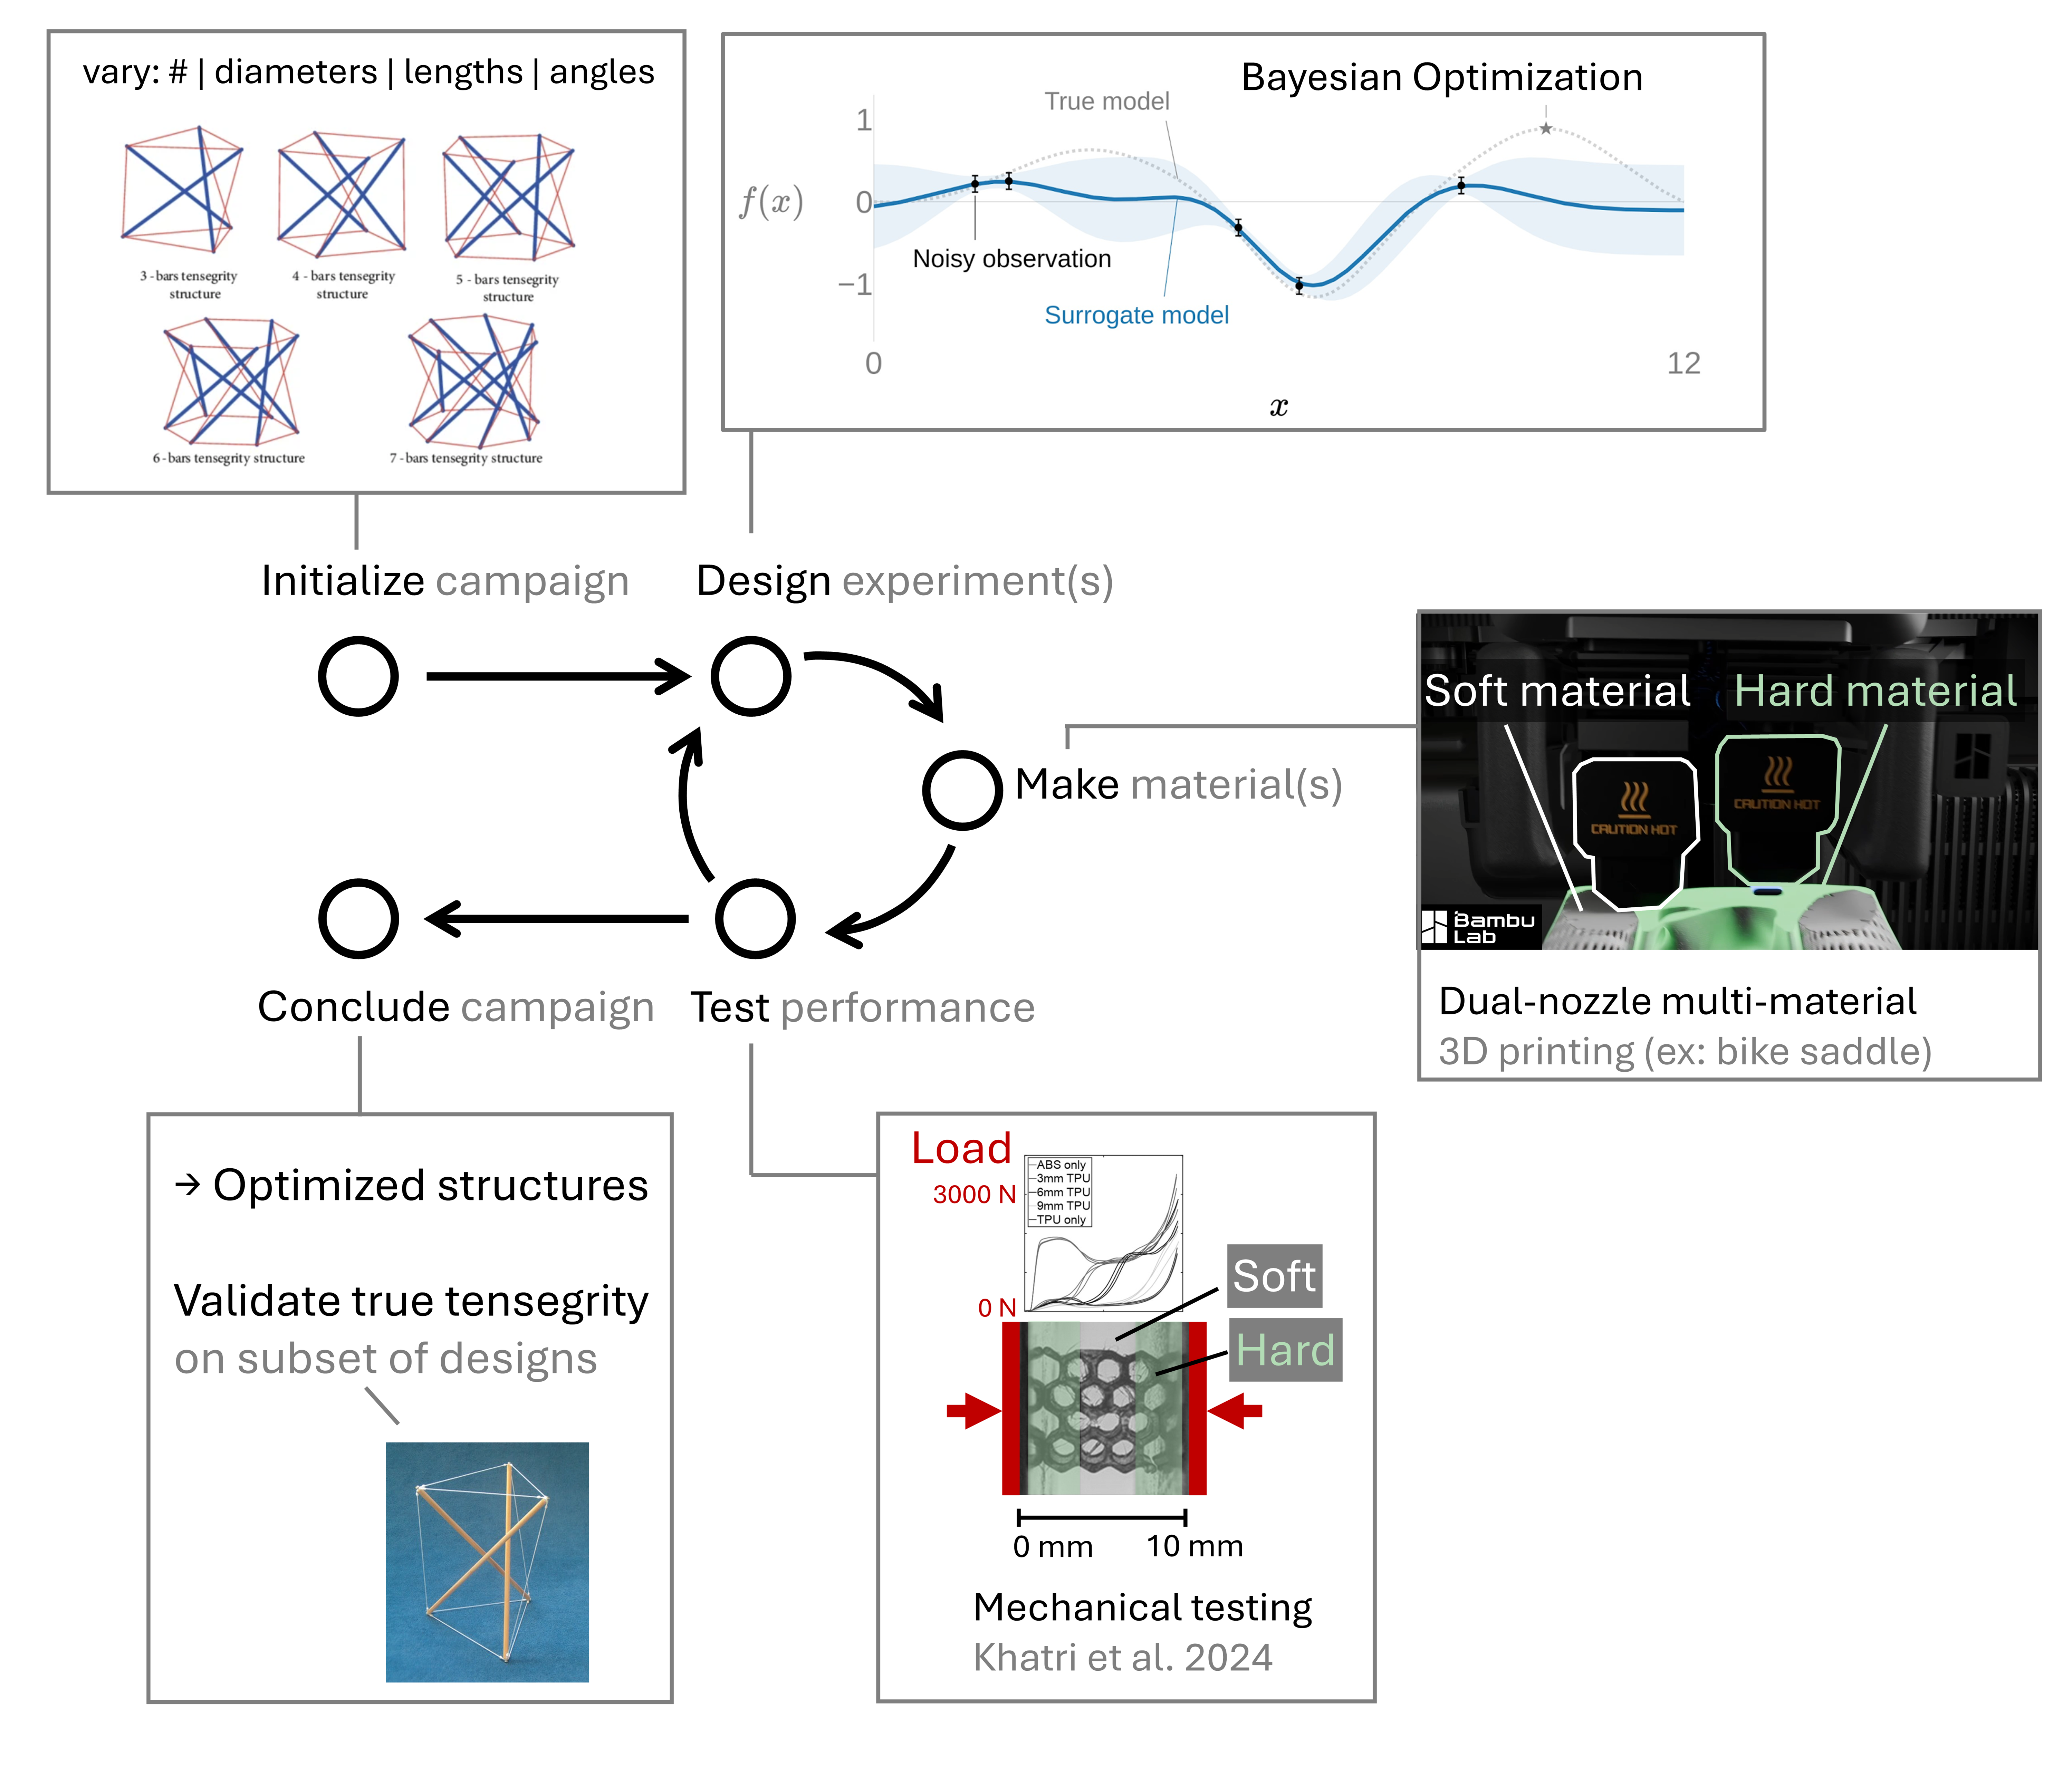
\includegraphics[width=0.7\textwidth]{../figures/overview-updated.png}
  \caption{Closed-loop, experiment-driven design framework. Parameterized
    PLA/TPU tensegrity-inspired unit cells are printed, characterized by
    repeated instrumented drop-weight impacts, and the resulting
    performance data drive a Gaussian-process surrogate that recommends the
    next batch of designs to fabricate.}
  \label{fig:overview}
\end{figure*}%
\todo{Eventually switch this overview figure to a vertical orientation; it is
  currently reproduced from the MRG proposal
  (\texttt{figures/overview-updated.png}).}

The remainder of the paper is organized as follows.
Section~\ref{sec:background} reviews tensegrity mechanics, multi-material
3D printing for energy absorption, and Bayesian optimization with an
emphasis on multi-objective and noise-robust acquisition functions.
Section~\ref{sec:methods} introduces the design parameterization,
fabrication workflow, drop-tower protocol and objectives, and BO loop,
and states the planned metal-analog comparison.
Section~\ref{sec:results} reports all four measured batches, the
surrogate audits, and the replication findings, and
Section~\ref{sec:discussion} discusses the
implications and limitations of the approach. Section~\ref{sec:conclusions}
concludes.

% =============================================================================
\section{Background}
\label{sec:background}
% =============================================================================

\subsection{Tensegrity-Inspired Architectures for Energy Absorption}

Tensegrity prisms and their planar extensions exhibit
softening-stiffening response under
compression~\citep{amendola2014experimental, zhang2018tensegrity,
fraternali2015tensegrity}, characteristics desirable for impact
mitigation because the structure can absorb a large fraction of the
input energy at a controlled, sub-injurious force plateau.
Santos~\cite{santos2023towardanovel} recently characterized a tensegrity
energy-dissipation metamaterial reporting equivalent viscous damping
on the order of $\sim$23\% with negligible residual strain per impact,
underscoring the suitability of tensegrity-inspired architectures for
repeated-impact use cases.
The space program literature documents large-scale tensegrity-inspired
absorbers for planetary landing~\citep{agogino2018superball,
caluwaerts2014superball, sabelhaus2015system, vespignani2018design,
deitrich2022titan} and a long history of crushable energy-absorbing
landing systems~\citep{cloutier1966landing, adams2004merairbag,
jackson2014honeycomb}. Pajunen et~al.~\cite{pajunen2019design} demonstrated that
truncated-tetrahedral tensegrity-inspired unit cells can be directly
3D-printed and exhibit load-limiting plateaus, motivating the present
focus on additively manufactured TPU/PLA composites.
More recent work on dynamically loaded additively-manufactured
energy-absorbing lattices~\cite{davami2019dynamicenergyabsorption}, together
with Intrigila et~al.'s bistable tensegrity-like unit cell for lattice
metamaterials~\cite{intrigila2022fabricationandexperimental} as the closest
published analog, confirms that this architecture class also responds favorably
under impact and quasi-static loading, although neither study employed
multi-material FDM or closed-loop design optimization.
Table~\ref{tab:novelty} situates the present work against selected
prior efforts spanning the three elements combined here (impact-tested
printed tensegrity-inspired structures, rigid-flexible fabrication,
and BO of architected materials), making explicit that, among the
studies reviewed, no single prior study combines a multi-material FDM
tensegrity-inspired architecture with an \emph{experiment}-driven
optimization loop.

\begin{table*}[t]
  \centering
  \caption{Positioning of this work against selected prior efforts
    spanning the elements combined here. The present campaign uses
    physical drop measurements of the transmissibility ($t_{180}$)
    and a mass-weighted rebound energy score ($E_{\mathrm{reb}}$)
    as its BO responses; it does not optimize specific energy
    absorption or crush energy.}
  \label{tab:novelty}
  \footnotesize
  \setlength{\tabcolsep}{4pt}
  \begin{tabular}{@{}llllll@{}}
    \toprule
    Study & Architecture & Fabrication & Optimization & Response optimized & Ground truth \\
    \midrule
    Pajunen et~al.\ 2019~\cite{pajunen2019design}
      & Truncated-tetrahedral & Single-material & None & n/a & Experiment \\
      & tensegrity-inspired & 3D print & (single condition) & & (drop impact) \\[2pt]
    Intrigila et~al.\ 2022~\cite{intrigila2022fabricationandexperimental}
      & Bistable tensegrity-like & Single-material & None & n/a & Experiment \\
      & lattice unit cell & 3D print & & & (quasi-static compr.) \\[2pt]
    Mo et~al.\ 2023~\cite{mo2023accelerated}
      & Architected lattices & n/a (simulation) & Multifidelity BO & Simulated response & Simulation \\
      & & & & metric & (+ sparse high-fid.) \\[2pt]
    Almeida 2025~\cite{almeida2025highstrainrate};
      & Tensegrity-inspired & Additive & None reported & n/a & Experiment \\
    \ \ Davami 2025~\cite{davami2025dynamicanalysis}
      & structures & manufacturing & & & (high-rate/dynamic) \\[2pt]
    Wang et~al.\ 2026~\cite{wang2026integrated}
      & Tensegrity-inspired & Integrated & None reported & n/a & Physical \\
      & rigid-flexible metamat. & dual-material & & & validation \\[2pt]
    \textbf{This work}
      & Tensegrity-inspired & Multi-material & Experiment-driven & $t_{180}$; provisional & Physical \\
      & $T_3$-prism cell (PLA/TPU) & FDM (PLA + TPU) & BO (SAASBO/qNEHVI) & $E_{\mathrm{reb}}$ & experiment \\
    \bottomrule
  \end{tabular}
\end{table*}


\subsection{Multi-Material 3D Printing of PLA/TPU Composites}

Multi-material rigid-soft FDM enables stiff/compliant combinations on a
single platform with tunable energy absorption, demonstrated for thick-panel
origami with PLA (or ABS/CFRP) panels and TPU hinges~\cite{ye2023multimaterial}
and for ABS-TPU honeycombs~\cite{khatri2024energy}. Neither study is itself a
tensegrity, but both establish the rigid-soft co-printing route we adopt. Ye
et~al.~\cite{ye2023multimaterial}
introduced a \emph{wrapping-based} strategy in which rigid cores are
encapsulated by continuous soft skins, reported to reduce interface
delamination under cyclic loading, something we take inspiration from in our
designs.
Beyond these rigid-soft demonstrations, a growing body of work confirms
that genuinely tensegrity-inspired architectures can be additively
manufactured and exhibit programmable mechanical response. Bauer
et~al.~\cite{bauer2021tensegrity} showed that 3D-printed tensegrity
metamaterials delocalize deformation to resist catastrophic failure, while
Pajunen et~al.~\cite{pajunen2021prestrain} tuned acoustic bandgaps in
3D-printed tensegrity-inspired lattices through prestrain, and
Sabouni-Zawadzka et~al.~\cite{sabounizawadzka2024experimental}
experimentally characterized 3D-printed tensegrity-inspired metamaterials
built on the simplex module. More directly relevant to impact, Almeida
et~al.~\cite{almeida2025highstrainrate} and Davami
et~al.~\cite{davami2025dynamicanalysis} characterized the high-strain-rate
and dynamic response of additively manufactured tensegrity-inspired
structures, and Wang et~al.~\cite{wang2026integrated} reported an
integrated fabrication-and-validation workflow for tensegrity-inspired
rigid-flexible metamaterials. Collectively these studies establish the
additive-manufacturability, tunability, and impact relevance of the
architecture class adopted here, none combining multi-material FDM with an
experiment-driven optimization loop.
Recent multi-material PLA/TPU sandwich and layered
composites~\citep{arifvianto2022mechanicalpropertiesof} report
quantitative bounds on
stiffness, strength, and energy absorption for the same PLA-TPU pair
used here, while FDM PLA fatigue
data~\citep{ezeh2018onthefatigue, vanaei2021multiscaledamageanalysis}
inform conservative design bounds for the rigid struts.
Architected multi-material lattices with co-printed compliant skins
have been explicitly designed for high specific energy
absorption~\citep{yavas2022designandfabrication}; recent surveys catalogue the
rapidly expanding additively manufactured polymeric energy-absorption
literature~\citep{bustihan2026recentadvancesin,
liu2026threedimensionalprintedlattice}. \todo{Add a short paragraph on
relevant TPU/PETG tensegrity search-space bounds once the Edison
literature task \texttt{5ae24eaf-5b6e-45cf-9f6c-1c7fbd881738}
synthesis is integrated.}

\subsection{Bayesian Optimization for Architected-Material Design}

Bayesian optimization is a sequential, model-based strategy for
optimizing expensive black-box functions using a Gaussian-process
surrogate~\citep{shahriari2016taking, frazier2018tutorial}. Modern
implementations such as BoTorch~\citep{balandat2020botorch} and the Ax
platform built atop it~\citep{pmlr-v293-olson25a} support
parallel batched evaluations and a wide variety of acquisition
functions; recent algorithmic advances include log-EI for numerical
robustness~\citep{ament2023logei}, noisy expected hypervolume
improvement for multi-objective settings~\citep{daulton2021nehvi},
input-noise-robust acquisitions~\citep{daulton2022robust}, and
evolution-guided constrained multi-objective BO for self-driving
labs~\citep{low2024evolution}. Mixed/categorical search spaces, needed
for the planned connectivity-topology extension rather than the
continuous $T_3$-prism prototype studied here, have dedicated
treatments in BOCS~\citep{baptista2018bocs} and the
one-hot-with-rounded-kernel construction
of~\citep{garridomerchan2020dealingwithcategorical}. BO has been
applied to architected-material
design~\citep{mo2023accelerated}
and to additive manufacturing~\citep{zhang2021bo}.
Mo et~al.~\cite{mo2023accelerated} in
particular established a multifidelity BO framework for architected
materials by fusing low-fidelity simulations with high-fidelity
ground truth via nonlinear information-fusion
priors~\citep{perdikaris2017nonlinear}; the present work shifts the
emphasis from simulation surrogates to direct experimental data,
appropriate for materials whose constitutive response is difficult to
calibrate from first principles.

% =============================================================================
\section{Materials and Methods}
\label{sec:methods}
% =============================================================================

\subsection{Design Parameterization}
\label{sec:methods:parameterization}

We parameterize a family of tensegrity-inspired unit cells via four
groups of design variables. For the working $T_3$-prism prototype that
defines the initial BO search space (Section~\ref{sec:methods:bo}),
only the first two groups are active and all of their variables are
\emph{continuous}; the connectivity-topology and tiling groups are
held fixed for this prototype and are listed here as planned
extensions of the design family:
\begin{itemize}
  \item \textbf{PLA compression members.} Strut diameter $d_s$ and
    length $\ell_s$, with the slenderness ratio $\ell_s / d_s$ bounded
    away from buckling-dominated regimes.
  \item \textbf{TPU tension elements.} Cross-sectional area $A_t$ (or
    equivalent diameter $d_t$ for circular cross-sections).
  \item \textbf{Connectivity topology (future extension).} Selected
    from a discrete set of candidate unit cells (e.g.,
    truncated-tetrahedral, prism-based, and octahedral variants); when
    activated, the design vector would encode this as a categorical
    choice. It is held fixed at the $T_3$ prism for the present
    campaign.
  \item \textbf{Unit-cell tiling (future extension).} Number of cells
    $N_x \times N_y \times N_z$ and the orientation of each cell
    relative to the impact direction; held fixed at a single cell here.
\end{itemize}
\todo{Specify exact manufacturing-feasibility constraints once
finalized; the connectivity-topology categorical encoding is deferred
until that variable is activated beyond the $T_3$ prism.}

\paragraph{Working prototype and search-space evolution} The first
instance of this family used to validate the fabrication and test
pipeline is a three-strut, $T_3$-prism-inspired cell scaled to a
$\sim$50\,mm bounding box. In batches 1 and 2 the BO harness exposes
five continuous design variables (base radius $R$, cell height $H$,
twist angle $\theta$, a single strut diameter $d_s$, and a single
cable (tendon) diameter $d_t$) over the ranges listed in
Table~\ref{tab:design-vars}; the cable diameter $d_t$ is treated as a
\emph{continuous} variable on $[3.0, 5.5]$\,\si{mm} rather than a
discrete set. From batch 3 the space grows to include the print
process: two per-article sparse-infill densities (strut and tendon,
each 12 to 35\%) chosen by the acquisition for every article, and
four filament settings (PLA and TPU nozzle temperature and maximum
volumetric speed) that are physically one value per print job, so
they are drawn as one quasi-random point per batch and are
acknowledged as confounded with batch until a round varies them
within a plate (Section~\ref{sec:methods:bo}). Under the prism's
$D_3$ symmetry all struts share one diameter and all cables share one
diameter, so the parameterization uses a single strut-diameter axis
and a single cable-diameter axis (two member-diameter axes), leaving
room to relax to per-orbit (saddle, top, bottom) or fully per-member
diameters once the individual orbits have been characterized.\todo{Cite the
heterogeneous-parameters Edison LITERATURE\_HIGH brief
(\texttt{5191cf4d}) on $D_3$-symmetric vs.\ fully-per-member
parameterization.} The joint diameter $d_j$ is held fixed at
\SI{7.0}{mm} rather than optimized: it sets the printed strut-end cage
that houses the internal cable anchors
(Section~\ref{sec:methods:fabrication}), so it is constrained primarily by the
TPU-tendon outlet count and the dual-nozzle clearance rather than by
energy-absorption performance, and fixing it keeps the anchor geometry
constant across specimens so that the optimized variables are not
confounded by joint-strength changes; relaxing $d_j$ is deferred to a
follow-on joint-design study. Figure~\ref{fig:printed-prototypes}
shows the parametric CAD model alongside an as-printed prototype of this
working $T_3$ prism.

\paragraph{Constant-mass projection and printability screens} Because
cell mass varies severalfold across the raw design box, an
unconstrained search would partly reward designs for carrying more
material rather than for their architecture. Every candidate is
therefore projected onto a constant material budget before printing:
the design is uniformly rescaled (all dimensions except the twist
angle) until its mass target is met, converged to within
\SI{0.15}{g} on rendered geometry. The target evolved with the
campaign. Batches 1 and 2 held \emph{solid} CAD mass
$\rho_{\mathrm{PLA}} V_{\mathrm{PLA}} + \rho_{\mathrm{TPU}}
V_{\mathrm{TPU}}$ at $m^{\star} = \SI{30.95}{g}$, the solid mass of
the reference prism. That budget does not hold printed grams
constant, because PLA struts print at partial infill while thin TPU
cables print near solid: as-printed masses spanned
\SIrange{18.50}{22.04}{g} across the tested seed articles
(coefficient of variation 5.5\%) and \SIrange{17.91}{23.47}{g}
(8.7\%) across batch 2, so the abstract's ``common mass budget'' is
approximate for those batches and the surrogate carries each
article's weighed mass explicitly
(Section~\ref{sec:methods:bo}). From batch 3 the projection instead
holds \emph{printed} mass at \SI{20.23}{g} (the reference article's
weight) by inverting the calibrated printed-mass model described in
the Supplementary Information; the achieved batch mass CVs were
1.7\% (batch 3) and 2.3\% (batch 4). Two printability screens are
evaluated on the projected geometry and recorded as flags rather
than hard rejections: a cylindrical build envelope
$\pi R^2 H \le \SI{250}{cm^3}$ and the \SI{3.0}{mm} TPU
self-bridging floor on the as-projected cable diameter (the
projection can scale a nominally feasible cable below the floor; the
two seed designs where this occurred both exhibited tendon stringing
defects, consistent with the screen, and the batch-4 attenuators
printed at 2.5 to \SI{2.8}{mm} with only minor stringing, so the
floor is a defect predictor rather than a hard failure line).

\begin{table}[ht]
  \centering
  \caption{Design variables for the $T_3$-prism campaign, as implemented
    in the BO harness. The seed batch is an $n=9$ Sobol draw (fixed
    seed) over the five geometry variables, with each design then
    projected onto the constant-mass budget of the text. The process
    variables joined the space in batch 3: the two infill densities
    are acquisition-chosen per article, while the four filament
    settings admit one value per print job and are therefore drawn as
    a single quasi-random point per batch (confounded with batch
    until varied within a plate). The joint diameter is held fixed.
    All specimens print in the vertical orientation on a Bambu
    Lab~H2D: one specimen per named build plate in the seed batch,
    one nine-article plate per batch thereafter.}
  \label{tab:design-vars}
  \small
  \begin{tabular}{@{}llccc@{}}
    \toprule
    Variable & Symbol & Units & Range & Active \\
    \midrule
    Base radius            & $R$       & mm  & 25-40 & batch 1 on \\
    Cell height            & $H$       & mm  & 60-110 & batch 1 on \\
    Twist angle            & $\theta$  & deg & 40-80 & batch 1 on \\
    Strut (PLA) diameter   & $d_s$     & mm  & 6.0-12.0 & batch 1 on \\
    Cable (TPU) diameter   & $d_t$     & mm  & 3.0-5.5 & batch 1 on \\
    Strut infill density   & -        & \%  & 12-35 & batch 3 on \\
    Tendon infill density  & -        & \%  & 12-35 & batch 3 on \\
    PLA nozzle temperature & -        & \si{\celsius} & 212-228 & batch 3 on\textsuperscript{a} \\
    PLA volumetric speed   & -        & \si{mm^3/s} & 20-30 & batch 3 on\textsuperscript{a} \\
    TPU nozzle temperature & -        & \si{\celsius} & 235-245 & batch 3 on\textsuperscript{a} \\
    TPU volumetric speed   & -        & \si{mm^3/s} & 2.2-3.6 & batch 3 on\textsuperscript{a} \\
    Joint diameter (fixed) & $d_j$     & mm  & 7.0 & - \\
    \bottomrule
  \end{tabular}\\[2pt]
  {\footnotesize \textsuperscript{a}One value per print job (a plate
  carries a single filament configuration), so per-batch rather than
  per-article.}
\end{table}%
\todo{The cable-diameter lower bound (3.0\,mm) is set by the Bambu
  auto-support detection floor; add the remaining
  manufacturing-feasibility constraints once finalized.}

\paragraph{As-built resolution of the continuous variables} Although
$d_s$ and $d_t$ are treated as continuous, the as-built cross-sections
are discretized by the nozzle diameter, the slicer line width, and
support interaction, so the effective search granularity is coarser
than the nominal continuous box. The realized member diameter therefore
changes in steps set by the line-width quantization rather than
continuously, and the smallest CAD change that yields a reliably
distinguishable as-built member is bounded below by these slicer
limits; the lower TPU-tendon bound (\SI{3.0}{mm}) is itself a
workflow-specific limit tied to the TPU self-bridging and auto-support
detection floor on this H2D platform rather than a fundamental
geometric one. The as-built quantity measured for every article is its
mass, weighed on a \SI{0.01}{g} scale; dimensional metrology of the
printed members has not yet been performed, so the geometry attached
to the surrogate is the commanded post-projection geometry. Two
print-to-print measurements bound the fabrication scatter: one seed
design printed in triplicate has a mass standard deviation of
\SI{0.457}{g}, and the full reprint of the batch-3 plate produced
nine design-replicate mass pairs whose second print weighed
\SI{0.27}{g} heavier article for article on average, a per-session
flow offset rather than random scatter. Both feed the observation
noise model (Section~\ref{sec:methods:bo}).

\begin{figure}[t]
  \centering
  \begin{subfigure}[b]{0.42\linewidth}
    \centering
    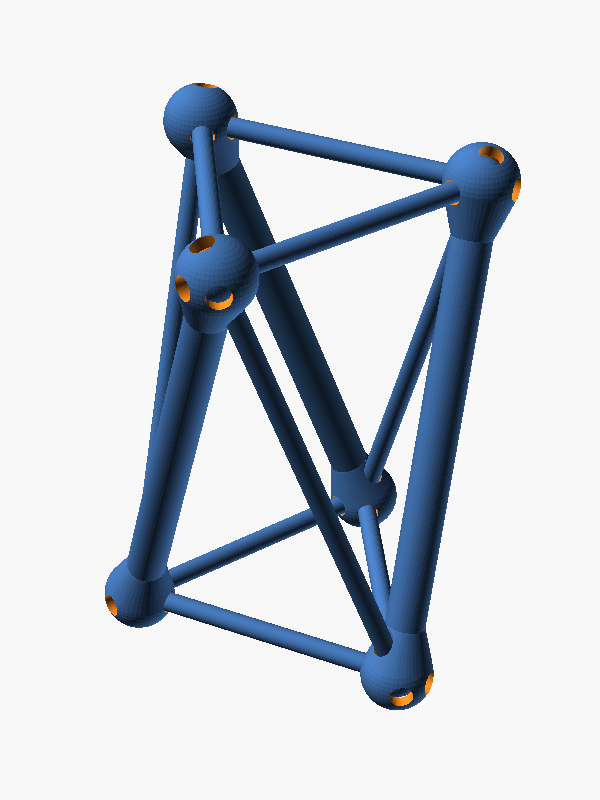
\includegraphics[width=\linewidth]{../figures/photos/cad-render.png}
    \label{fig:proto-cad}
  \end{subfigure}\hfill
  \begin{subfigure}[b]{0.54\linewidth}
    \centering
    \begin{tikzpicture}
      \node[anchor=south west,inner sep=0] (ph)
        {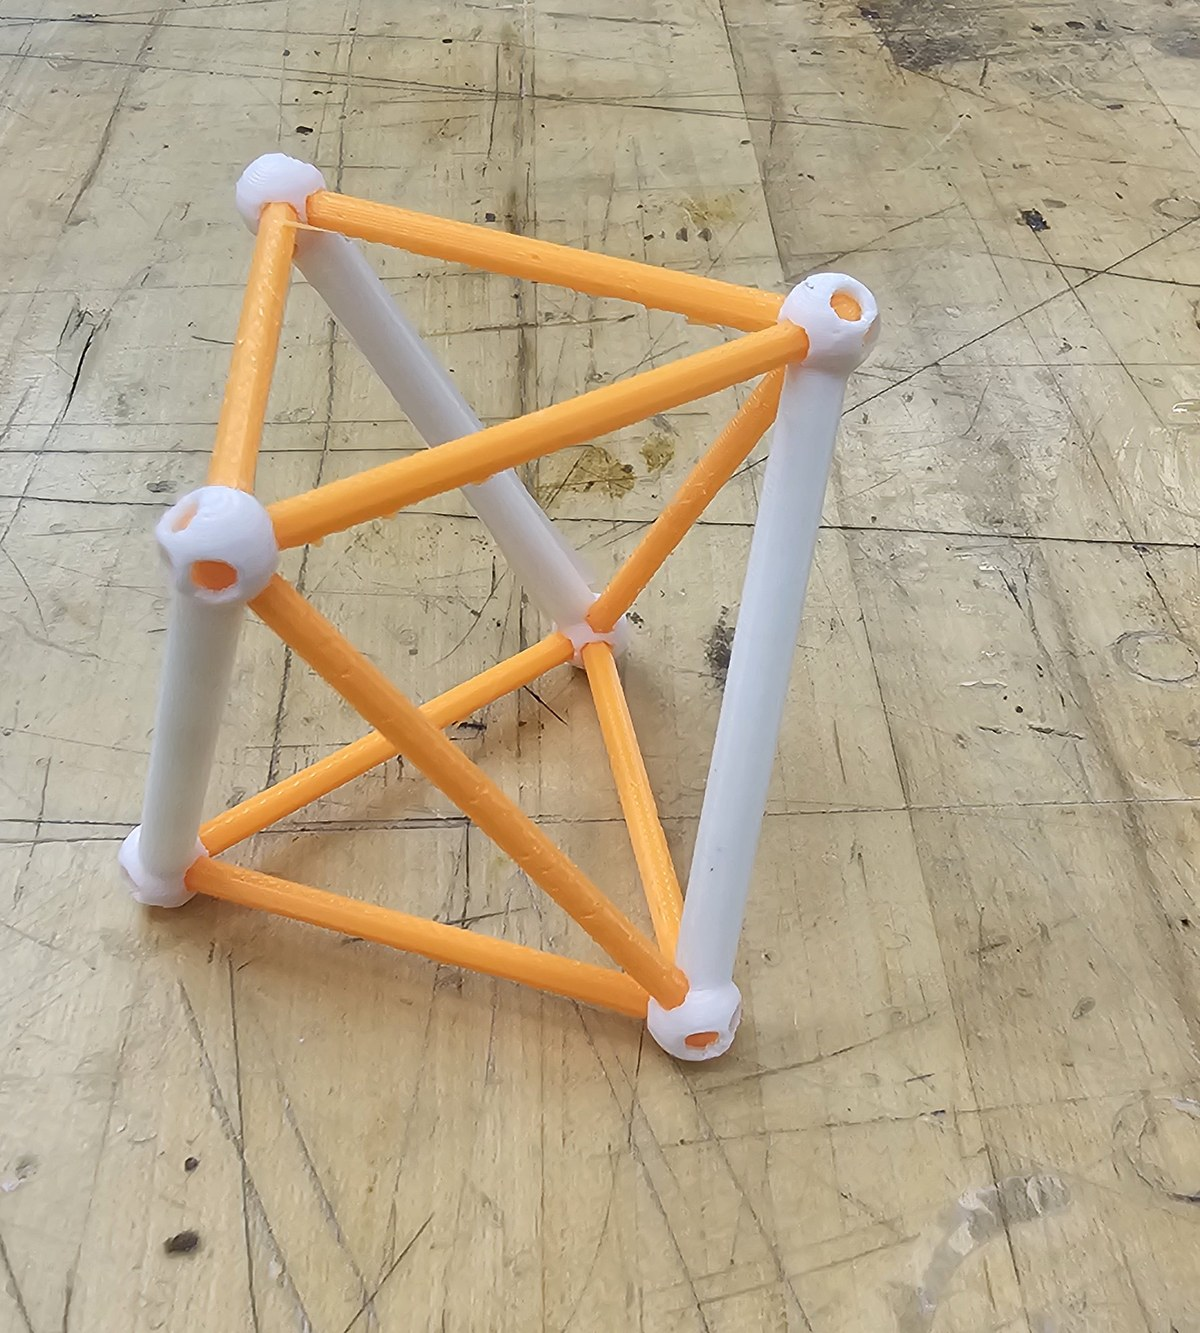
\includegraphics[width=\linewidth]{../figures/photos/printed-specimen.jpg}};
      \begin{scope}[x={(ph.south east)},y={(ph.north west)},
                    font=\sffamily\scriptsize]
        \tikzset{callout/.style={-{Latex[length=1.5mm]},line width=0.5pt,
                                 draw=red!75!black}}
        \tikzset{lab/.style={fill=white,fill opacity=0.85,text opacity=1,
                             inner sep=1pt,rounded corners=1pt}}
        \draw[callout] (0.74,0.95) node[lab,anchor=south]{$d_s$}
          -- (0.63,0.52);
        \draw[callout] (0.22,0.96) node[lab,anchor=south]{$d_t$}
          -- (0.34,0.70);
        \draw[{Latex[length=1.5mm]}-{Latex[length=1.5mm]},line width=0.5pt]
          (0.05,0.23) -- (0.05,0.85) node[lab,midway]{$H$};
      \end{scope}
    \end{tikzpicture}
    \label{fig:proto-print}
  \end{subfigure}
  \caption{Working $T_3$-prism prototype. \emph{(a)} Parametric OpenSCAD model
    whose base radius $R$, cell height $H$, twist angle $\theta$, strut diameter
    $d_s$, and cable diameter $d_t$ are the design variables of
    Table~\ref{tab:design-vars}. \emph{(b)} A representative dual-material print
    from the PR~\#35 print history (rigid PLA struts, here in white; tendon
    members in orange), with callouts marking the strut diameter $d_s$, a tendon
    (cable) diameter $d_t$, and the cell height $H$; the inter-plate twist
    $\theta$ is the relative rotation of the top and bottom node triangles, and
    the base radius $R$ sets their circumradius.}
  \label{fig:printed-prototypes}
\end{figure}

\subsection{Multi-Material Fabrication}
\label{sec:methods:fabrication}

Specimens are fabricated on a multi-material FDM printer using PLA for
the rigid struts and TPU for the soft tension elements.
Figure~\ref{fig:fab-workflow} summarizes the end-to-end fabrication and
characterization workflow, from parametric CAD through multi-material
slicing, dual-extrusion printing, post-processing, and mechanical
testing. Rather than
wrapping the struts in a continuous TPU skin, the current design anchors
the TPU tension elements \emph{inside} the ends of each PLA strut: the
cables converging at a given strut end are joined within the strut,
which acts as a rigid cage housing the junction, and the individual
tendons then exit through discrete outlets. This keeps the soft-rigid
interface in internal, compression-dominated pockets rather than at an
exposed overmolded surface. This construction effectively inverts the
material roles of Ye et~al.'s soft-skin-over-rigid-core
wrapping~\cite{ye2023multimaterial}: here a soft TPU core is captured within
a rigid PLA shell, so we cite that work only as a multi-material co-printing
precedent rather than as validation of the present junction. \todo{Quantitatively
verify the internal-anchoring junction strength against the PR~\#39 / PR~\#35
joint pull-out studies before making any cyclic-durability claim.} \todo{Document slicer profile
(layer height, infill, print speed, nozzle temperatures, retraction
settings) and validation prints used to characterize PLA-TPU interface
strength.}

\paragraph{Print platform and joint geometry} The working platform is
a Bambu Lab~H2D printer, which permits a single rigid-soft build
without filament swaps. Strut endpoints are tied to cables through
parametric joint geometries developed and ranked through a five-design
OpenSCAD study (anchor-bulb, dovetail, TPU-sleeve overmold,
eyelet-loop, and TPU-rebar variants); the working prototype uses a
dovetail joint (Design~B) with an anchor-bulb backup (Design~A) for
sensitivity studies, with a captive TPU core routed inside the PLA
shell to keep the soft tendon protected from layer-line failure at
the strut-to-cable transition. The full five-design comparison and the
selected junction are detailed in the Supplementary Information.\todo{Cite the
joint-design Phase-3 CAD review (Edison ANALYSIS \texttt{19e0c868}) and the
Phase-4 vision review (\texttt{e9a1f4cc}) once both are integrated into the
references.}

\paragraph{Supports for soft members} Because near-vertical TPU
tendons are otherwise unsupported during printing, automatic support
generation is disabled and supports are painted manually in the
slicer: PLA edge supports run along each tendon, with the
support-to-object clearance tightened from \SI{0.35}{mm} to
\SI{0.2}{mm} during tuning on the reference prism. Two support-removal
artifacts recur in the seed batch (surface stringing and, on two
articles, TPU strands pulled off bottom tendons during support
removal) and are logged per article in the print key (Supplementary
Information). An automated alternative (a lowered support-threshold
angle plus mesh-ray-cast narrowing pillars) was developed in parallel
and is documented in the Supplementary Information.

\paragraph{Moisture and nozzle management} TPU is hygroscopic, so the
soft filament is fed from a heated dry box held near \SI{8}{\percent}
relative humidity, logged per print. Midway through the seed batch the
TPU extruder developed a progressive flow taper (a partial clog,
compounded by a stray PLA fragment found inside the extruder); it was
resolved by a cold pull and by moving the TPU to a dedicated
high-flow \SI{0.6}{mm} nozzle, after which print quality was restored.
The affected and post-fix articles are identified in the print key so
that any nozzle-related covariate can be checked against the measured
objectives.

\begin{table}[ht]
  \centering
  \caption{Multi-material print parameters on the Bambu Lab~H2D,
    transcribed from the archived as-printed Bambu Studio project
    (\texttt{t3-prism-bo-batch.H2D-MM-PLAstruts-TPUcables.as-printed.3mf},
    Bambu Studio 2.7.1). Filaments are Bambu Lab PLA Basic (struts,
    support material) and Bambu Lab TPU~85A (tendons); the print
    profile is ``0.30\,mm Standard @BBL H2D 0.6 nozzle.'' The
    reporting structure follows the methods section of Ye
    et~al.~\cite{ye2023multimaterial}.}
  \label{tab:print-params}
  \small
  \setlength{\tabcolsep}{3pt}
  \begin{tabular}{@{}lcc@{}}
    \toprule
    Parameter & PLA (struts) & TPU 85A (tendons) \\
    \midrule
    Nozzle                             & \SI{0.6}{mm} & 0.4 then \SI{0.6}{mm} HF\textsuperscript{a} \\
    Nozzle temperature (\textdegree C) & 220 & 220 \\
    Bed temperature, profile (\textdegree C) & 55 & 35 \\
    Layer height / line width (mm)     & \multicolumn{2}{c}{0.30 / 0.62} \\
    Infill                             & 15\% grid, 2 walls & near-solid \\
    Outer / inner wall speed (mm/s)    & \multicolumn{2}{c}{200 / 300 (profile)} \\
    Filament drying                    & n/a & dry box, $\sim$8\% RH \\
    Build-plate type                   & \multicolumn{2}{c}{Textured PEI} \\
    Build orientation                  & \multicolumn{2}{c}{Vertical} \\
    Supports                           & \multicolumn{2}{c}{Manual painted tree supports, PLA} \\
    \bottomrule
  \end{tabular}\\[2pt]
  {\footnotesize \textsuperscript{a}The TPU side ran a standard
  \SI{0.4}{mm} nozzle until the mid-batch clog, then a dedicated
  high-flow (HF) \SI{0.6}{mm} nozzle; affected articles are flagged in
  the print key.}
\end{table}%
\todo{@achris0520 to confirm the physical nozzle hardware (the
  archived as-printed project records \SI{0.6}{mm} on both extruders,
  consistent with the post-fix state; the TPU side ran \SI{0.4}{mm}
  before the mid-batch nozzle change logged in the print key) and to
  supply filament lot numbers and drying duration, which the slicer
  archive does not record.}

\begin{figure*}[t]
  \centering
  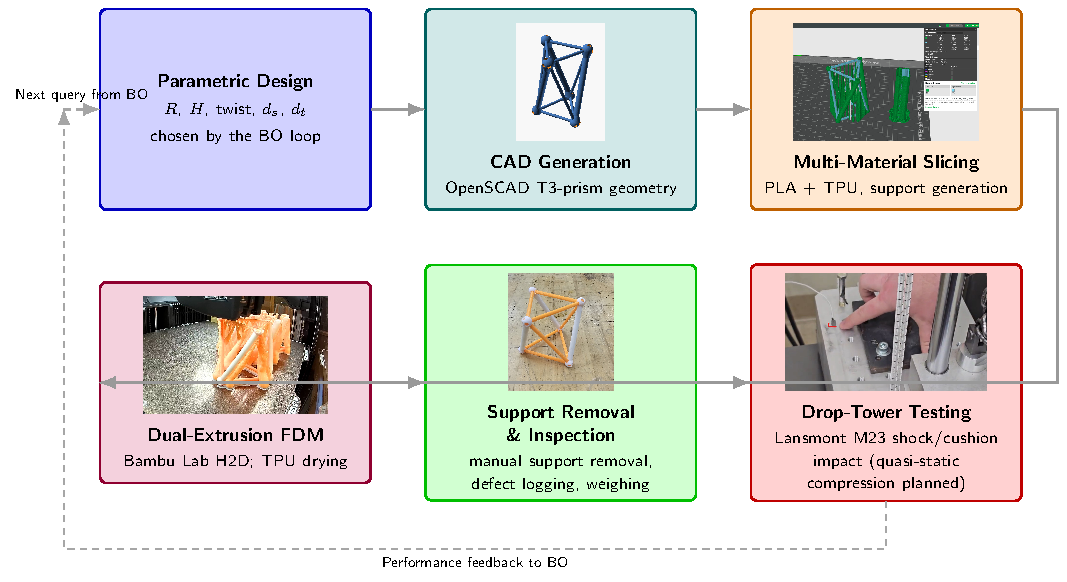
\includegraphics[width=\textwidth]{../figures/fab-workflow.pdf}
  \caption{Fabrication and characterization workflow for the multi-material
    tensegrity-inspired unit cells: design parameters drive parametric CAD,
    slicing with manually generated TPU supports, a single multi-material
    print on the Bambu Lab~H2D, post-processing and inspection, and
    mechanical testing. Node photographs are representative artifacts drawn
    from the project's build history: the OpenSCAD $T_3$-prism render
    (CAD), the dual-nozzle Bambu Studio slice with PLA on the left extruder
    and TPU on the right (slicing), an in-progress H2D print of the prism
    batch (FDM), an as-printed specimen (post-processing), and the
    bungee-assisted drop-tower base plate with accelerometer (testing).}
  \label{fig:fab-workflow}
\end{figure*}%

\subsection{Experimental Characterization}
\label{sec:methods:testing}

\paragraph{Drop-tower fixture} The primary characterization is
repeated drop-weight impact on a Lansmont Model~23 shock test system.
The printed specimen rides upright on the carriage plate, which is
raised \SI{60}{in} (\SI{1.524}{m}) along guide rails and released; the
plate lands on a single \SI{0.5}{in} Shore 60~OO polyurethane cushioning
sheet, which shapes the landing into a single sharp base pulse of
roughly \SI{1.6}{ms} duration. This impact-surface configuration was
selected by a blinded crossover experiment over three candidate mat
arrangements, and unlike a felt stack it does not measurably compact
over hundred-drop sessions. Rig health is monitored continuously
through the impact velocity change $\Delta v$ recovered from the base
accelerometer: over an uninterrupted 100-drop characterization session
the $\Delta v$ coefficient of variation was 0.54\% with no drift, and
every campaign session is checked against the healthy tower baseline
(details, including the within-session mat warm-up and recovery
pattern, in the Supplementary Information). One drop takes roughly
\SI{42}{s}, so a seed-batch characterization completes in about
ninety minutes per article and a later-batch session in about
fifteen.

\paragraph{Instrumentation and signal processing} A single-axis
piezoelectric accelerometer on the carriage plate records the base
input and triggers the acquisition; a triaxial accelerometer (Dytran
3133A4) seated in a printed pocket at the specimen's top vertex records
the transmitted response. The two base-capable channels were
cross-calibrated in place over fifteen co-located drops (ratio
$0.953 \pm 0.001$ at matched filtering), and the transducer settings
are archived with the data. Signals are captured at
\SI{1.25}{MHz} over a \SI{100}{ms} record with a \SI{2}{ms}
pre-trigger. All channels are low-pass filtered with the SAE~J211/1
channel-frequency-class (CFC) filters~\citep{saej211}, implemented from
the standard's published coefficients with the two-pass corner
frequency handled explicitly (a common implementation shortcut narrows
the passband by roughly 20\%, which we identified and corrected before
the campaign; all reported numbers use the corrected filter). CFC-180
is the reporting class for peak metrics, with CFC-1000 retained as a
higher-bandwidth diagnostic.

\paragraph{Per-article objectives and session protocol} Session
length evolved with the campaign's understanding of its own noise,
and the per-batch counts are stated here because they differ. Seed
sessions recorded 103 drops per article and contribute 101 stabilized
captures each (103 for one article, autv5r) after the first two drops
of each session are discarded as seating warm-up. A pre-campaign
variance study on the commissioning datasets put the statistical
minimum at five stabilized drops after two warm-ups, and the seed
sessions confirmed that the stabilized mean is insensitive to session
length: within-session per-drop CVs of 0.17 to 0.48\% with flat
post-warm-up trends, and a replay of the seed sessions truncated to
twenty drops leaves the transmissibility ranking of all eight tested
articles unchanged, with a worst-case mean shift of $+0.008$ against
design-to-design gaps of 0.007 to 0.087 and a per-drop standard
error still an order of magnitude below those gaps. Later sessions
were therefore shortened to about twenty drops per article: the
committed record lists 21 to 22 valid captures per batch-2 article
and 20 recorded drops per article in batches 3 and 4, against 101
valid captures per seed article, with the first two drops of every
session discarded as before (exact per-session counts are in the
archived per-drop records). The shortening cuts tower time per
article
from about ninety minutes to about fifteen while retaining roughly
four times the minimum stabilized-drop budget; a shorter session
simply enters the surrogate with a proportionally larger standard
error, which the model downweights. The second print-and-test pass
of batch 3
(Section~\ref{sec:results:batches}) subsequently confirmed that
seating and print variation, not session length, limit what a
session can claim, so the freed tower time goes to re-seats. Each
session yields two objectives, each reported as a stabilized mean
with the per-drop scatter quoted as one standard deviation; the
standard error of the mean is what enters the surrogate's noise model
(Section~\ref{sec:methods:bo}):
\begin{equation}
  \begin{aligned}
    t_{180} &\;=\; \frac{\max_t\,\lVert \mathbf{a}_{\mathrm{top}}(t)\rVert_{\mathrm{CFC180}}}
                        {\max_t\,\lvert a_{\mathrm{base}}(t)\rvert_{\mathrm{CFC180}}},\\
    E_{\mathrm{reb}} &\;=\; e_{\mathrm{reb}}\, m\, g\, h,
    \qquad
    e_{\mathrm{reb}} \;=\; \frac{g\, t_{\mathrm{second}}}{2\,\Delta v},
  \end{aligned}
  \label{eq:objectives}
\end{equation}
where $t_{180}$ is the CFC-180 filtered peak-acceleration ratio,
which we name once here and then call the \emph{transmissibility}
throughout: the peak magnitude of the triaxial top-vertex response
over the peak base input within the impact window. The term is used
in the shock-testing sense standard for cushioning and packaging
drop tests, a ratio of filtered peak accelerations across the
article under a single transient, not the steady-state
frequency-response function of vibration isolation: the two peaks
need not be simultaneous, the filter class is part of the
definition, and SAE~J211/1 is cited only for the impact-channel
filtering. Values above unity indicate the structure amplifies the
peak shock reaching its top vertex; values below unity indicate
attenuation. $E_{\mathrm{reb}}$ is a \emph{provisional
mass-weighted rebound score} with units of energy (millijoules per
drop): the dimensionless rebound fraction $e_{\mathrm{reb}}$ is
recovered from the ballistic timing of the top vertex's post-impact
hop~\citep{bernstein1977listening} ($t_{\mathrm{second}}$ is the time
to the second contact event and $\Delta v$ the measured base velocity
change), and it is scaled by each article's own weighed mass $m$ and
the drop height $h$. Two interpretive caveats are deliberate. The
ballistic reading of the second contact event has not yet been
validated against synchronized video, and $\Delta v$ is the base
plate's velocity change rather than a demonstrated incident relative
velocity, so $e_{\mathrm{reb}}$ is a rebound-timing score rather than
a coefficient of restitution; and because a strict restitution reading
would scale returned kinetic energy as the \emph{square} of a velocity
ratio, $E_{\mathrm{reb}}$ is a mass-aware ranking score that penalizes
designs (and grams) that throw more motion back at the payload, not a
measured rebound energy. The score is the campaign's second
objective through all four batches and remains a candidate to become
a constraint once validated
(Section~\ref{sec:discussion}). Using the mass-weighted form rather
than the bare fraction keeps the objective mass-aware: equal fractions
on articles of different printed mass are not equivalent outcomes for
a payload. Ringdown descriptors (the fitted natural frequency $f_n$,
260 to \SI{470}{Hz} for every article but one batch-4 design that
rings at \SI{764}{Hz}, and, where
the exponential fit passes an $r^2 \ge 0.85$ gate, a damping ratio
$\zeta$) are recorded per drop as print-health and prestress
diagnostics~\citep{ashwear2014natural} but are not campaign objectives.
The within-session per-drop CV of $t_{180}$ spans 0.06 to 2.0\%
across the campaign's 35 articles (0.17 to 0.48\% in the seed
batch). These
values describe repeated drops of the same physical article in one
seating and do not estimate print-to-print or seating-to-seating
repeatability; serial dependence among drops may also make
$s/\sqrt{n_{\mathrm{drops}}}$ optimistic. Two replication
measurements bound what a single session can claim: the seed
attenuator re-measured across a day and an independent re-seat
agreed to 0.13\%, while a full second print-and-test pass of the
batch-3 plate showed same-design shifts with a median of $+1.2\%$
and heavy tails (Section~\ref{sec:results:batches}). The campaign
therefore adopted a between-seat replication rule: a single-seating
value that would drive a decision (a batch extreme, a claimed
attenuator, a front membership) requires confirmation on an
independent re-seat before it is treated as a design property. A
mechanism-oriented trace figure (processed
deceleration response with event markers keyed to synchronized video
frames) will be generated from archived campaign captures once the
event labels can be supported by synchronized measurements; no such
figure is shown here because none of the required event
synchronization has yet been performed.

\paragraph{Planned quasi-static extension} The drop test loads the
specimens in their elastic regime (the crush lasts 1 to \SI{3}{ms} and
the article recovers), so crush-energy metrics such as specific energy
absorption (SEA) and compaction efficiency are not recoverable from
these captures by any reprocessing. A quasi-static compression
campaign on a benchtop load frame (BYU CB~123 Instron, with a
low-range load cell appropriate to the expected cell stiffness)
is planned to supply the complementary crush metrics
\begin{equation}
  \mathrm{SEA} \;=\; \frac{1}{m}\!\int_{0}^{\delta_d}\! F(\delta)\,
  \mathrm{d}\delta,
  \qquad
  \eta_c \;=\; \frac{\int_{0}^{\delta_d}\! F(\delta)\,\mathrm{d}\delta}{F_{\max}\,\delta_d},
\end{equation}
with the densification displacement $\delta_d$ taken at the maximum of
the energy-absorption efficiency curve and $F_{\max}$ the peak force
within $[0,\delta_d]$, following the canonical cellular-solid
treatments~\citep{gibson1997cellular, avalle2001characterization,
tan2005dynamic, michailidis2011establishment} and mirroring the
quasi-static protocol of Pajunen et~al.~\citep{pajunen2019design}.
These metrics are reported as a complementary characterization of
selected designs rather than as objectives of the drop-tower campaign.
Slip resistance and traction at the specimen-to-floor interface,
governed by the tip geometry rather than the internal architecture,
follow ISO 11334-4~\citep{iso11334-4} for walking-aid tips and are out
of scope for the present axial-impact study.

\paragraph{Complementary data streams} High-speed video
(\SI{959}{fps}, three clips per specimen) supplements the
accelerometer data. The camera cannot resolve the millisecond-scale
impact pulse (one to two frames), so the division of labor is
explicit: the accelerometer channels produce the objectives, and video
documents the post-impact rebound and recovery. Synchronized
laser-Doppler vibrometry is reserved for follow-up characterization of
selected designs.

\subsection{Experiment-Driven Bayesian Optimization Loop}
\label{sec:methods:bo}

The optimization loop maintains a Gaussian-process (GP) surrogate over
the design space defined in
Section~\ref{sec:methods:parameterization}. After each round of
physical experiments, the surrogate is refit and an acquisition
function is maximized to recommend the next batch of designs to
fabricate. The campaign is posed as a two-objective minimization:
simultaneously minimize the transmissibility $t_{180}$
and the per-drop rebound energy $E_{\mathrm{reb}}$ of
Eq.~\eqref{eq:objectives}. Both objectives serve the same payload:
$t_{180}$ bounds the peak shock it feels during the impact, and
$E_{\mathrm{reb}}$ penalizes the motion thrown back into it afterward.
The seed data showed an apparent trade-off driven substantially by
the single strongest attenuator, not statistically resolved at seven
mapped articles (Spearman $\rho = -0.39$, $p = 0.38$;
Section~\ref{sec:discussion}); the measured front after four batches
is nondegenerate (its members span both axes), and the rebound axis
remains a candidate to become a constraint once its ballistic
reading is validated.
Implementation
uses the Ax platform~\citep{pmlr-v293-olson25a} over
BoTorch~\citep{balandat2020botorch}, with noisy expected hypervolume
improvement (qNEHVI)~\citep{daulton2021nehvi} as the multi-objective
acquisition. The $T_3$-prism search space is fully continuous,
including the process variables added in batch 3
(Table~\ref{tab:design-vars}), so no categorical
encoding is required; the mixed-search-space constructions
of~\citep{garridomerchan2020dealingwithcategorical} and the BOCS
combinatorial baseline~\citep{baptista2018bocs} remain the route for
the future connectivity-topology categorical rather than part of the
current loop. The input-noise-robust acquisition of Daulton
et~al.~\cite{daulton2022robust} and the evolution-guided constrained
variant of Low et~al.~\cite{low2024evolution} are held in reserve as
contingencies.

\paragraph{Surrogate and noise model} The surrogate is the fully
Bayesian sparse axis-aligned subspace model
(SAASBO)~\citep{eriksson2021saasbo}: a Mat\'ern-5/2 kernel with
automatic relevance determination whose length scales carry strong
sparsity-inducing priors and are marginalized by Markov-chain Monte
Carlo (NUTS) rather than point-estimated; every refit in the
campaign, through the batch-4 ingestion, uses this model with qNEHVI
on top (Ax 0.4 for the early rounds, Ax~0.5.0 from the batch-3
refit). We retain SAASBO even though the
dimensionality is modest because marginalizing the hyperparameters
tends to improve uncertainty quantification at the very small sample
sizes of physical campaigns; the fitted model is audited each round
with leave-one-out cross-validation and length-scale-based
sensitivity diagnostics
(Section~\ref{sec:results}). Inputs are normalized to the unit cube
and outputs standardized. Observation noise is supplied per
observation as a fixed variance: for $t_{180}$ the squared standard
error of the stabilized mean,
$\sigma_t^2 = s_{\mathrm{drop}}^2 / n_{\mathrm{drops}}$, and for the
rebound score the drop-scatter term plus the propagated
print-to-print mass scatter,
$\sigma_E^2 = \sigma_{E,\mathrm{drops}}^2 +
(\partial E_{\mathrm{reb}}/\partial m)^2 \sigma_m^2$ with
$\sigma_m = \SI{0.457}{g}$ measured from the one design printed in
triplicate; a shorter session enters with a proportionally larger
standard error. The estimand this noise model implies is the
response of the tested article in its seating, not of a freshly
printed article at the same design: an independent adversarial
review (Section~\ref{sec:discussion}) argued the decision-relevant
target is the latter, and the campaign's response is the measured
replication evidence of Section~\ref{sec:results:batches} (a full
second print-and-test pass of one batch) together with the
between-seat replication rule, rather than an inflated per-article
noise term. SAASBO is the
prespecified surrogate; we make no claim that it outperforms
a standard single-task GP at this dimensionality and sample size,
and the planned head-to-head calibration comparison against a
point-estimated GP with the same kernel remains future work.

\paragraph{Mass treatment} Because the constant \emph{solid}-mass
projection of batches 1 and 2 does not hold printed grams constant
(Section~\ref{sec:methods:parameterization}), printed mass correlates
with the shape variables in the seed batch ($r = 0.83$, $n = 7$,
dominated by the lightest article, against $t_{180}$). The loop
therefore makes mass explicit rather than pretending it away: the
rebound objective is expressed in absolute millijoules using each
article's weighed mass, so added grams are re-penalized through the
energy they deliver back to the payload, while $t_{180}$ deliberately
stays a ratio because payload peak acceleration is a damage criterion
that does not scale with specimen mass. The objective surrogates take
the design coordinates of Table~\ref{tab:design-vars} as their
inputs; printed mass is attached as a separately modeled
\emph{tracking metric}, so the model learns as-printed mass as a
function of the design coordinates and every recommendation reports a
predicted printed mass (the diagnostic refit behind
Fig.~\ref{fig:sensitivity} additionally includes printed mass as an
input, precisely to probe this confound). The calibrated
printed-mass model of the Supplementary Information closed the loop
on this compromise: batches 3 and 4 hold \emph{printed} grams
constant, and the mass-transmissibility correlation across the 26
articles of batches 1 to 3 fell to $r = 0.07$, so the confound the
seed batch raised was broken by design rather than adjusted away in
analysis.

\paragraph{Budget and seeding} The seed batch is an $n = 9$ Sobol
draw with a recorded seed over the five-variable box, printed together
with the fixed reference prism (S0). Optimization proceeds in
sequential batches of $q = 9$ prints, sized to one build-plate
generation cycle. Three model-recommended batches are reported here
(Ax trials 10 to 18, 28 to 36, and 37 to 45; the numbering gap
records a superseded draft batch that was regenerated, before
printing, when the batch-level filament handling was simplified).
From batch 3 the four filament settings take one quasi-random point
per batch, formally the settings of that batch's best-predicted
article, so those axes are confounded with batch and are reported as
unidentified rather than learned. All random seeds,
the full experiment state, and the recommendation tables are recorded
per round; full computational reproducibility (the exact processing
pipeline and model settings) is carried by the campaign code, whose
archival release is a declared submission gate rather than a solved
item. Escalation to
trust-region BO (TuRBO)~\citep{eriksson2019turbo} is planned only if
per-member-diameter extensions push the design space well beyond the
present regime; a single-objective log-Expected-Improvement
run~\citep{ament2023logei} on $t_{180}$ is retained as a baseline for
quantifying the benefit of the multi-objective formulation. The
campaign code and recommended batches will be archived at a
Zenodo-minted DOI mirroring the GitHub repository.\todo{Insert the
Zenodo DOI and release version for the campaign code once the
repository snapshot is published.}

\subsection{Replicate Rank-Stability Study}
\label{sec:methods:rankstability}

The batch-3 second pass (Section~\ref{sec:results:batches}) showed
that a single article's measurement can move between seatings and
prints by more than the design signal separating neighboring
articles, which bounds any claim that one design outranks another. A
planned replicate study formalizes that bound by re-printing a
deliberately spread subset of the already-measured designs. Among
the campaign's in-sample designs, ranked by the current posterior's
predictions, we will select the best-predicted design, the
worst-predicted design, and one mid-pack (``run-of-the-mill'')
design, then print a nominal three fresh articles of each (the
repeat count, provisionally three, will be fixed when the print is
scheduled) and drop-test every article under the standard protocol
of Section~\ref{sec:methods:testing}, including the between-seat
replication rule. The question is whether the predicted ordering
survives fabrication and seating variation. With three designs the
exact permutation floor for a Spearman rank correlation is
$p = 1/6$, so no significance claim is available at this size;
the primary readout is instead the separation of the three designs'
repeat clusters relative to the within-design (print-to-print plus
seat-to-seat) scatter, reported alongside $\rho_s$ between the
predicted and measured orderings of each repeat. Clean separation
would support treating the campaign's rankings as design properties;
overlapping clusters would localize the ranking noise floor that the
batch-3 second pass could only bound. The reporting format is
specified in Table~\ref{tab:rank-stability}; entries and design IDs
will be added once the repeat articles are printed and tested.

\begin{table}[ht]
  \centering
  \caption{\emph{Placeholder (data pending).} Planned replicate
    rank-stability study: the best-, mid-, and worst-predicted
    in-sample designs, each re-printed as a nominal three fresh
    articles and drop-tested under the standard protocol. Entries
    will record each repeat's stabilized $t_{180}$, the
    within-design scatter, and the measured rank of each design's
    repeat cluster against its predicted rank.}
  \label{tab:rank-stability}
  \small
  \begin{tabular}{@{}llcccc@{}}
    \toprule
    Tier & Design & {Pred.\ $t_{180}$} &
    \multicolumn{3}{c}{$t_{180}$ (repeats 1 / 2 / 3)} \\
    \midrule
    Best  & \textit{TBD} & \textit{-} & \textit{-} & \textit{-} & \textit{-} \\
    Mid   & \textit{TBD} & \textit{-} & \textit{-} & \textit{-} & \textit{-} \\
    Worst & \textit{TBD} & \textit{-} & \textit{-} & \textit{-} & \textit{-} \\
    \bottomrule
  \end{tabular}
\end{table}%
\todo[inline,color=orange!30]{Populate Table~\ref{tab:rank-stability}
  once the repeat articles of the best-, mid-, and worst-predicted
  in-sample designs are printed and drop-tested; fix the repeat count
  (nominally three) and the design IDs when the print is scheduled.}

\subsection{Metal-Analog Validation}
\label{sec:methods:validation}

In the future we plan a validation campaign that tests whether the
rankings learned on the printed PLA/TPU specimens generalize beyond
the as-printed polymer system, by reproducing a subset of the
$T_3$-prism designs as
\emph{metal analogs} built from hollow aluminum rods (compression
members) and stainless-steel threaded cables (tension members), using
the same $R$, $H$, $\theta$, and member-diameter parameterization.
Rather than fabricating only the top-ranked geometries, we
deliberately span the predicted performance range: a few designs the
surrogate predicts to be \emph{worst}-performing, a few
\emph{mediocre}, and a few \emph{best}-performing are each built in
both material systems. Comparing the measured ordering of the
PLA/TPU specimens against their hollow-aluminum/stainless-steel
counterparts probes whether both systems preserve the same
rank ordering of impact performance. We treat this as a
\emph{planned, exploratory} comparison rather than a preregistered
validation: the deformation modes, joint compliance,
friction, pretension behavior, and strain-rate sensitivity all differ
between the PLA/TPU and aluminum/steel systems, so agreement is not
expected a priori, and the protocol details that would let the
comparison distinguish geometric rank transfer from material-system
and mass confounds (aluminum alloy and temper, tube wall thickness,
cable construction, joint hardware and torque, article and payload
masses, replicate count, and tie-handling rules) remain to be fixed
and will be tabulated before any metal article is built. The intended
rank statistic is the Spearman rank-correlation coefficient $\rho_s$
between the two
material systems' orderings of the primary campaign metric ($t_{180}$
under the identical drop protocol), reported with an exact permutation
test, with the provisional rebound score
$E_{\mathrm{reb}}$ and, once the quasi-static extension runs, SEA
reported as secondary rankings. Rank agreement would be preliminary
evidence consistent with transfer; disagreement would not isolate
which material or joint difference caused the change.
The planned reporting format is specified in
Table~\ref{tab:metal-validation}; the table entries and the specimen
photographs of Fig.~\ref{fig:metal-validation} will be added after
fabrication and testing.

\begin{table}[ht]
  \centering
  \caption{\emph{Placeholder (data pending).} Planned rank-ordering
    validation: representative $T_3$-prism designs predicted to be
    worst-, mid-, and best-performing, each fabricated as a printed
    PLA/TPU specimen and as a hollow-aluminum-rod / stainless-steel-cable
    metal analog. Entries record the measured performance metric
    ($t_{180}$ under the identical drop protocol, with the provisional
    rebound score secondary) and the resulting rank within each
    material system; rank agreement would be preliminary evidence
    consistent with transfer, while disagreement would not isolate
    which material or joint difference caused the change.}
  \label{tab:metal-validation}
  \begin{tabular}{@{}llcc@{}}
    \toprule
    Predicted tier & Design ID & PLA/TPU (rank) & Al/SS (rank) \\
    \midrule
    Worst    & \textit{D-w1} & \textit{-} & \textit{-} \\
    Worst    & \textit{D-w2} & \textit{-} & \textit{-} \\
    Mediocre & \textit{D-m1} & \textit{-} & \textit{-} \\
    Mediocre & \textit{D-m2} & \textit{-} & \textit{-} \\
    Best     & \textit{D-b1} & \textit{-} & \textit{-} \\
    Best     & \textit{D-b2} & \textit{-} & \textit{-} \\
    \bottomrule
  \end{tabular}
\end{table}%
\todo[inline,color=orange!30]{Populate Table~\ref{tab:metal-validation}
  with measured metrics and ranks once the metal-analog validation
  specimens (hollow Al rods + stainless-steel threaded cables) and their
  PLA/TPU equivalents have been built and tested.}

\figplaceholder{metal-validation}{Assembled validation specimens for
  each predicted performance tier (worst / mediocre / best), shown as
  printed PLA/TPU builds alongside their hollow-aluminum-rod and
  stainless-steel-threaded-cable metal analogs, with callouts marking
  the aluminum compression members, the threaded steel tension cables,
  and the strut-end cable anchors. Photographs to be added once the
  specimens are fabricated.}

% =============================================================================
\section{Results}
\label{sec:results}
% =============================================================================

\subsection{Seed-Batch Measurements}
\label{sec:results:seed}

All nine Sobol specimens and the reference prism were printed and
declared acceptable to test. Nine articles (seven mapped Sobol
designs, the reference prism, and one article whose design mapping
is unconfirmed) completed seed characterization sessions, totaling
over 900 clean captures within a project-wide history of more than
4{,}000 instrumented drops; the two remaining seed designs (specs 03
and 06) were printed, but their drop sessions are absent from the
campaign record and they do not enter any fit or figure.
Table~\ref{tab:seed-results} reports the
stabilized objectives. Three findings frame the batch. First, the
measured $t_{180}$ spans 0.893 to 1.062: six of nine tested articles
\emph{amplify} the peak shock reaching the top vertex (means above
unity), two sit marginally below unity (0.997 and 0.980), and one
tested article (the print of Sobol spec~01, the thick-strut,
thin-cable, high-twist corner of the batch) had a mean $t_{180}$ of
0.893, indicating peak attenuation under the tested condition. This
article's attenuation later reproduced across an independent re-seat
to 0.13\%, the campaign's positive control for the replication rule
of Section~\ref{sec:methods:testing}.
Across the tested articles, $t_{180}$ spans 0.169 (18.9\% of
the observed minimum). This between-article range far exceeds the
0.17 to
0.48\% within-session per-drop CV, but one mechanically tested
article per geometry does not permit separation of geometry effects
from print-to-print variation or other fabrication covariates.
Second, the objectives show an
apparent trade-off in this sample: the best attenuator carries the
largest rebound score (13.9~mJ per drop), so the observed front is
nondegenerate, although the trade-off is driven substantially by that
single article and is not statistically resolved at this sample size
(Section~\ref{sec:discussion}). Third, among the eight mapped
articles with weighed masses, printed mass and $t_{180}$ showed a
large sample
correlation ($r = 0.82$, $n = 8$). The association is confounded with
the design coordinates and is highly sensitive to the lightest
article ($r = 0.26$ when 6lhxfy is omitted); it is not evidence of a
causal mass effect. It nonetheless motivated the mass-aware objective
formulation of Section~\ref{sec:methods:bo}, and the
constant-printed-mass batches later broke the confound outright
(Section~\ref{sec:results:audits}). Figure~\ref{fig:seed-designs} renders
the seed geometries to a common scale, showing how widely the
constant-mass box spans aspect ratio, member sizing, and twist.

\begin{figure}[t]
  \centering
  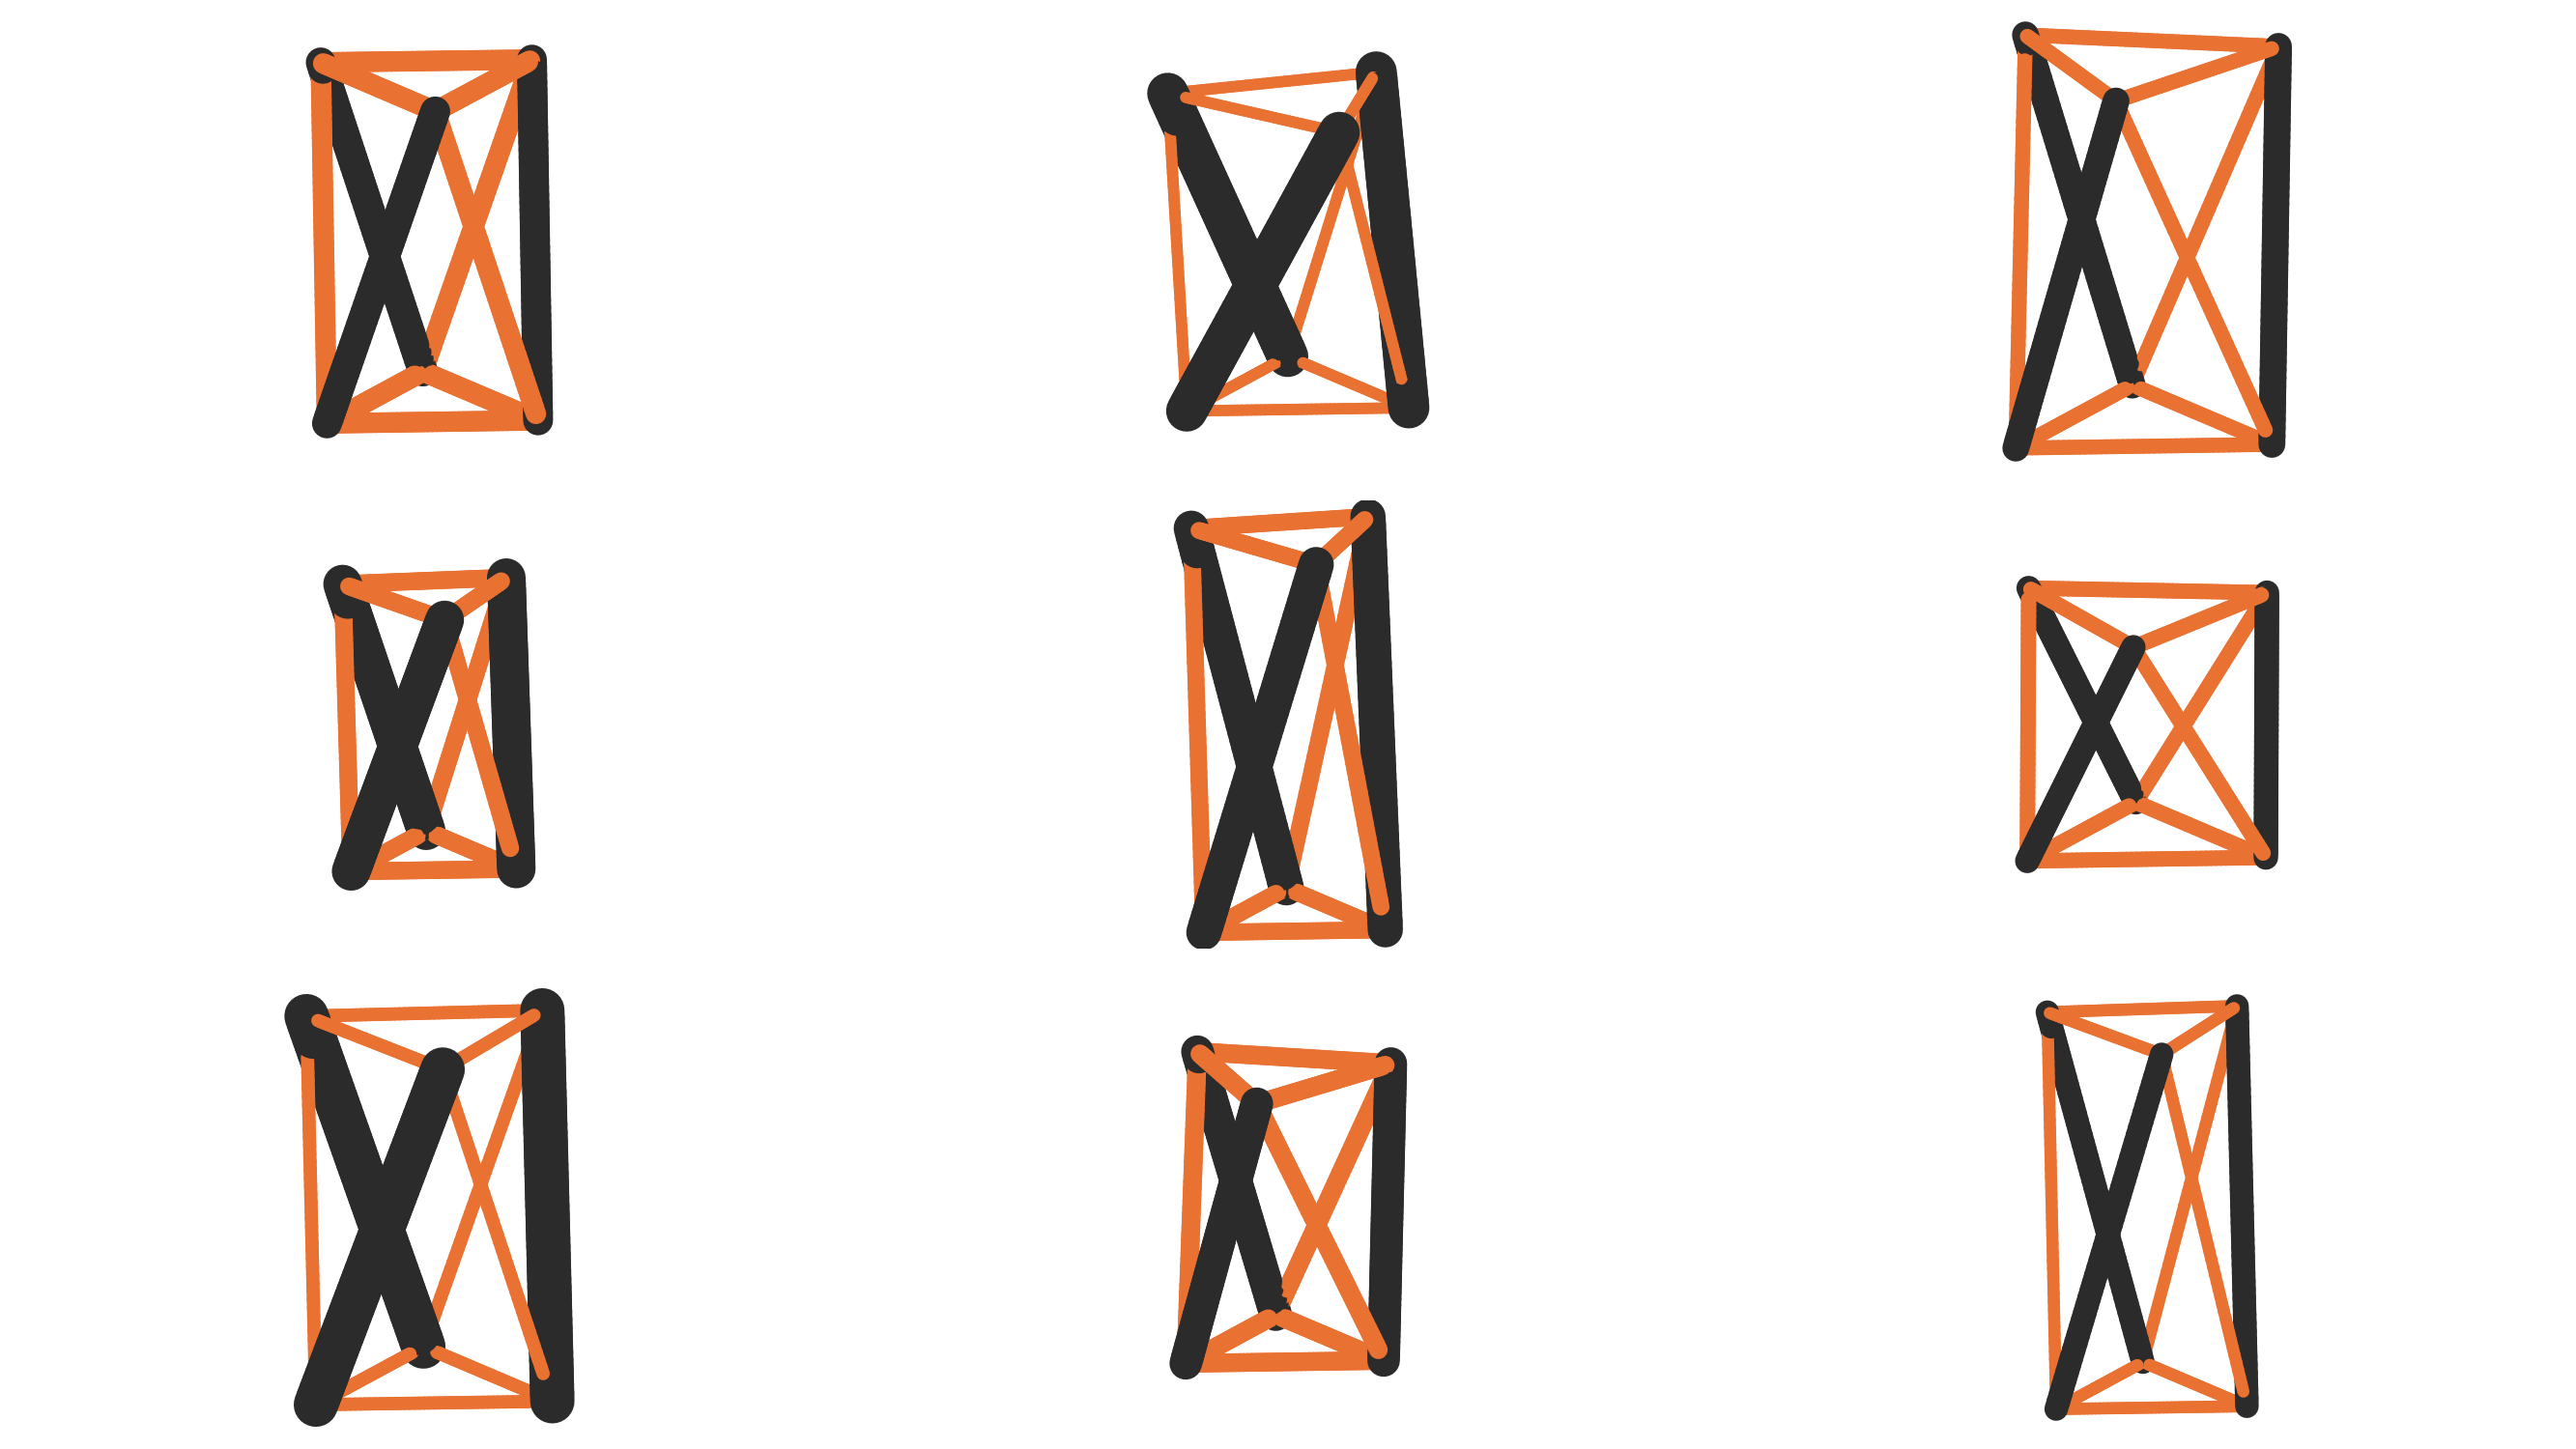
\includegraphics[width=\linewidth]{../figures/bo/fig-seed-designs.png}
  \caption{The nine seed geometries rendered to a common millimeter
    scale (rigid PLA struts in black, TPU tendons in orange). Every
    rendering corresponds to a physically printed article in the seed
    campaign.}
  \label{fig:seed-designs}
\end{figure}

\begin{table*}[t]
  \centering
  \caption{Seed-batch drop-tower results: 101 stabilized captures per
    article (103 for autv5r) at \SI{60}{in} onto the standardized
    polyurethane surface, CFC-180 filtering, counted after the first
    two warm-up drops of each session were discarded. Means $\pm$ one
    standard deviation over the stabilized drops; rows are ordered by
    $t_{180}$. $E_{\mathrm{reb}}$ uses each
    article's weighed mass per Eq.~\eqref{eq:objectives}. The ringdown
    frequency $f_n$ is a print-health descriptor, not an objective.
    A dash denotes a quantity that cannot be computed from the
    available record: article \textit{amdjwm} lacks a weighed mass and
    a confirmed design mapping (it is excluded from the surrogate fit
    and from all mass-dependent quantities), and no accepted $f_n$
    estimate is available for \textit{bag26v} or \textit{ajhby6}.
    Specs 03 and 06 were printed but have no drop sessions in the
    campaign record.}
  \label{tab:seed-results}
  \small
  \begin{tabular}{@{}llS[table-format=2.2]S[table-format=1.4]@{\,$\pm$\,}S[table-format=1.4]S[table-format=2.1]S[table-format=3.0]@{}}
    \toprule
    Design & Article & {Mass (g)} & \multicolumn{2}{c}{$t_{180}$} &
    {$E_{\mathrm{reb}}$ (mJ)} & {$f_n$ (Hz)} \\
    \midrule
    Spec 01 & 6lhxfy & 18.50 & 0.8931 & 0.0042 & 13.9 & 368 \\
    (unmapped) & amdjwm & {-} & 0.9805 & 0.0025 & {-} & 455 \\
    Spec 05 & 6nheas & 21.73 & 0.9970 & 0.0032 & 13.1 & 322 \\
    S0 ref. & bpx68c & 20.23 & 1.0111 & 0.0024 & 6.2 & 468 \\
    Spec 07 & ajhby6 & 20.53 & 1.0127 & 0.0038 & 6.1 & {-} \\
    Spec 00 & 9hhbkp & 21.62 & 1.0183 & 0.0017 & 6.9 & 364 \\
    Spec 04 & nvxsrv & 20.66 & 1.0275 & 0.0044 & 8.2 & 294 \\
    Spec 02 & autv5r & 22.04 & 1.0404 & 0.0035 & 8.8 & 386 \\
    Spec 08 & bag26v & 21.42 & 1.0616 & 0.0051 & 7.7 & {-} \\
    \bottomrule
  \end{tabular}
\end{table*}

\subsection{Model-Recommended Batches and Replication}
\label{sec:results:batches}

Table~\ref{tab:batch-results} reports the stabilized objectives for
the three model-recommended batches, and
Fig.~\ref{fig:front-evolution} overlays every measured article with
the non-dominated front after each batch (Pareto membership is
evaluated over articles with both objectives; the unmapped seed
article amdjwm is omitted because its missing weighed mass prevents
computing $E_{\mathrm{reb}}$). Dominated hypervolume, evaluated at
the fixed reference point $(t_{180}, E_{\mathrm{reb}}) =
(1.35, \SI{15}{mJ})$, grew from 3.155 after the seed batch to 3.969
after batch 2 ($+25.8\%$), 4.007 after batch 3 ($+0.9\%$), and 5.195
after batch 4 ($+29.7\%$): a 65\% total gain over the seed front. No
budget-matched quasi-random physical baseline has been run, so the
comparison the data support is against the campaign's own Sobol
seed: after batch 4, every member of the combined front (corny7,
corny6, drran5, drran3, r2d2c6) is a model-recommended design, and
the last seed article left the front when the batch-4 record
dominated it outright.

\paragraph{Batch 2 (Ax trials 10 to 18)} The first recommended batch
was generated from the seed fit and printed under the
constant-solid-mass projection, so its printed masses still spread
widely (17.91 to \SI{23.47}{g}; a regenerated constant-printed-mass
recommendation set is archived alongside the as-printed one, and the
two must not be conflated). The batch grew the front almost entirely
on the rebound axis: r2d2c6's \SI{4.1}{mJ} per drop is the lowest
rebound on record and still stands, and four batch-2 articles joined
the front. On the transmissibility axis the batch humbled its own
forecasts: the archived posterior predictions sat below the
measurements for nine of nine articles (mean absolute percentage
error 14.4\%; worst case r2d2c3, predicted 0.910, measured 1.334,
the strongest amplifier in the campaign record). That nine-of-nine
optimism widened the refit posterior for every batch that followed.

\paragraph{Batch 3 (Ax trials 28 to 36)} The first batch at constant
\emph{printed} mass (19.24 to \SI{20.06}{g}, CV 1.7\%) and the first
with the infill and filament axes active
(Section~\ref{sec:methods:parameterization}). It filled the knee of
the front rather than growing the box ($+0.9\%$ hypervolume; three
articles joined), and the recalibrated posterior held: eight of nine
articles measured within 0.3 posterior standard deviations of their
predictions (MAPE 3.8\%). The batch also delivered the campaign's
sharpest single surprise in both directions: the best-predicted
design (trial 32, predicted 1.020) measured 1.251, the strongest
amplification then on record, while the batch's only attenuator
(drran8, 0.980, drift-flagged, provisional) was its only twisted
design.

\paragraph{Batch 4 (Ax trials 37 to 45)} The acquisition split the
batch between the wide, high-twist, thin-cable family it had been
steering toward since batch 2 and a previously unvisited tall,
low-twist corner. The wide family delivered: four of nine articles
attenuate, and corny7, the batch's best-predicted design (trial 37,
predicted $0.934 \pm 0.13$), measured $t_{180} = 0.8031 \pm 0.0025$,
the strongest attenuation in the program, 10\% below the best seed
article and 21\% below the reference prism, at a mid-pack
\SI{9.4}{mJ} rebound; it dominates the seed attenuator on both
objectives (Fig.~\ref{fig:batch4-pred-vs-meas}). Within the
attenuating family the frozen predictions ranked the four
measurements perfectly (Spearman $\rho = +1.0$; $0.82$ across all
nine, where the five amplifier predictions span only 0.9\% and so
carry no ordering signal), batch MAPE was 6.0\%, and no article left
its predictive band by more than one standard deviation (the record
itself beat its band by 1.0 standard deviation in the good
direction). Per the between-seat replication rule, the batch-4
attenuation values, including the record, are single-seating
measurements whose re-seat confirmations are scheduled; one session
(corny5) carries a drift flag and its mean is provisional, and
another (corny6) was erratic (per-drop CV 2.0\%) but attenuates
under any reading of its record.

\paragraph{Replication: a second pass of batch 3} The batch-3 plate
was printed a second time (nine design replicates, the reprint
weighing \SI{0.27}{g} heavier article for article on average) and
the second set was drop-tested under the identical protocol, 360
drops across the two passes. Neither extreme of the first pass
recurred. Under \emph{any} pairing of the blinded session labels,
the design that measured 1.251 re-measured at most 1.090 (a drop of
at least 13\%) and the 0.980 attenuator re-measured at least 1.011,
so batch 3 contains no reproducibly attenuating design; under the
best-fit pairing, the same-design shifts have median $+1.2\%$, five
of nine fall inside the previously characterized $\pm 2.2\%$ re-seat
envelope, and the tails reach $-13.8\%$. The two passes cannot
separate seating effects from print-to-print differences, but the
methodological conclusion does not depend on that split: the 1.251
session had passed every within-session stability check (per-drop CV
0.77\%, no drift), so \emph{within-session stability does not
certify a measurement as a design property}. The between-seat
replication rule of Section~\ref{sec:methods:testing} was adopted in
response, the seed attenuator's 0.13\% agreement across an
independent re-seat shows that genuine attenuation does reproduce,
and a broadband seat gauge (the ratio of CFC-1000 to CFC-180
transmissibility; healthy sessions read 1.00 to 1.07) now
accompanies the rule as an advisory: every large same-design shift
observed so far carried a gauge reading of at least 1.15 in one of
its seatings, and all four batch-4 attenuators gauge healthy (0.98
to 1.06).

\begin{table*}[t]
  \centering
  \caption{Model-recommended batch results under the protocol and
    reporting conventions of Table~\ref{tab:seed-results} (CFC-180,
    stabilized means $\pm$ one standard deviation; about twenty
    drops per article against the seed batch's 101, with exact
    per-session counts in the archived per-drop records; rows
    ordered by $t_{180}$ within each batch).
    $E_{\mathrm{reb}}$ uses each article's weighed mass per
    Eq.~\eqref{eq:objectives}. ``Pred.'' is the posterior-mean
    $t_{180}$ archived when the batch was recommended, before any of
    its articles were tested. Batch-2 articles were projected to
    constant solid mass; batches 3 and 4 to constant printed mass
    (\SI{20.23}{g}). Flags follow the session record: $\dagger$
    marks a transmissibility-drift-flagged session whose mean is
    provisional, and $\ddagger$ marks the erratic corny6 session
    (per-drop CV 2.0\%).}
  \label{tab:batch-results}
  \small
  \begin{tabular}{@{}clcS[table-format=2.2]S[table-format=1.4]@{\,$\pm$\,}S[table-format=1.4]S[table-format=2.1]S[table-format=1.3]@{}}
    \toprule
    Batch & Article & Trial & {Mass (g)} & \multicolumn{2}{c}{$t_{180}$} &
    {$E_{\mathrm{reb}}$ (mJ)} & {Pred.\ $t_{180}$} \\
    \midrule
    2 & r2d2c7 & 15 & 18.51 & 0.9484 & 0.0008 & 12.2 & 0.905 \\
    2 & r2d2c1 & 13 & 19.38 & 0.9942 & 0.0021 & 6.0 & 0.948 \\
    2 & r2d2c2$^\dagger$ & 12 & 17.96 & 1.0411 & 0.0154 & 5.6 & 0.926 \\
    2 & r2d2c9 & 10 & 17.91 & 1.0530 & 0.0035 & 5.8 & 0.873 \\
    2 & r2d2c6 & 14 & 19.11 & 1.0548 & 0.0042 & 4.1 & 0.953 \\
    2 & r2d2c8 & 17 & 19.98 & 1.0704 & 0.0116 & 7.9 & 0.955 \\
    2 & r2d2c5 & 18 & 23.47 & 1.1516 & 0.0040 & 6.7 & 0.987 \\
    2 & r2d2c4 & 11 & 19.33 & 1.1847 & 0.0076 & 6.4 & 0.885 \\
    2 & r2d2c3 & 16 & 18.63 & 1.3337 & 0.0117 & 5.6 & 0.910 \\
    \midrule
    3 & drran8$^\dagger$ & 35 & 19.32 & 0.9804 & 0.0051 & 11.2 & 1.039 \\
    3 & drran1 & 36 & 19.31 & 1.0326 & 0.0016 & 18.1 & 1.051 \\
    3 & drran4 & 29 & 19.92 & 1.0344 & 0.0017 & 9.1 & 1.032 \\
    3 & drran2 & 33 & 19.33 & 1.0345 & 0.0006 & 11.8 & 1.056 \\
    3 & drran5 & 28 & 19.88 & 1.0373 & 0.0024 & 5.0 & 1.059 \\
    3 & drran3 & 31 & 19.92 & 1.0389 & 0.0012 & 4.2 & 1.043 \\
    3 & drran9 & 30 & 19.34 & 1.0425 & 0.0009 & 5.2 & 1.058 \\
    3 & drran6 & 34 & 19.24 & 1.0471 & 0.0040 & 4.8 & 1.065 \\
    3 & drran7 & 32 & 20.06 & 1.2513 & 0.0096 & 8.2 & 1.020 \\
    \midrule
    4 & corny7 & 37 & 19.62 & 0.8031 & 0.0025 & 9.4 & 0.934 \\
    4 & corny9 & 43 & 19.46 & 0.8766 & 0.0036 & 18.1 & 0.942 \\
    4 & corny6$^\ddagger$ & 41 & 19.45 & 0.9106 & 0.0181 & 5.7 & 0.943 \\
    4 & corny8 & 39 & 19.64 & 0.9535 & 0.0025 & 17.5 & 0.954 \\
    4 & corny1 & 42 & 20.20 & 1.0459 & 0.0029 & 8.7 & 1.010 \\
    4 & corny4 & 44 & 20.56 & 1.0475 & 0.0025 & 4.3 & 1.013 \\
    4 & corny3 & 45 & 20.15 & 1.0705 & 0.0013 & 8.8 & 1.004 \\
    4 & corny2 & 38 & 20.21 & 1.0846 & 0.0030 & 9.2 & 1.008 \\
    4 & corny5$^\dagger$ & 40 & 20.58 & 1.0876 & 0.0099 & 8.5 & 1.012 \\
    \bottomrule
  \end{tabular}
\end{table*}

\begin{figure*}[t]
  \centering
  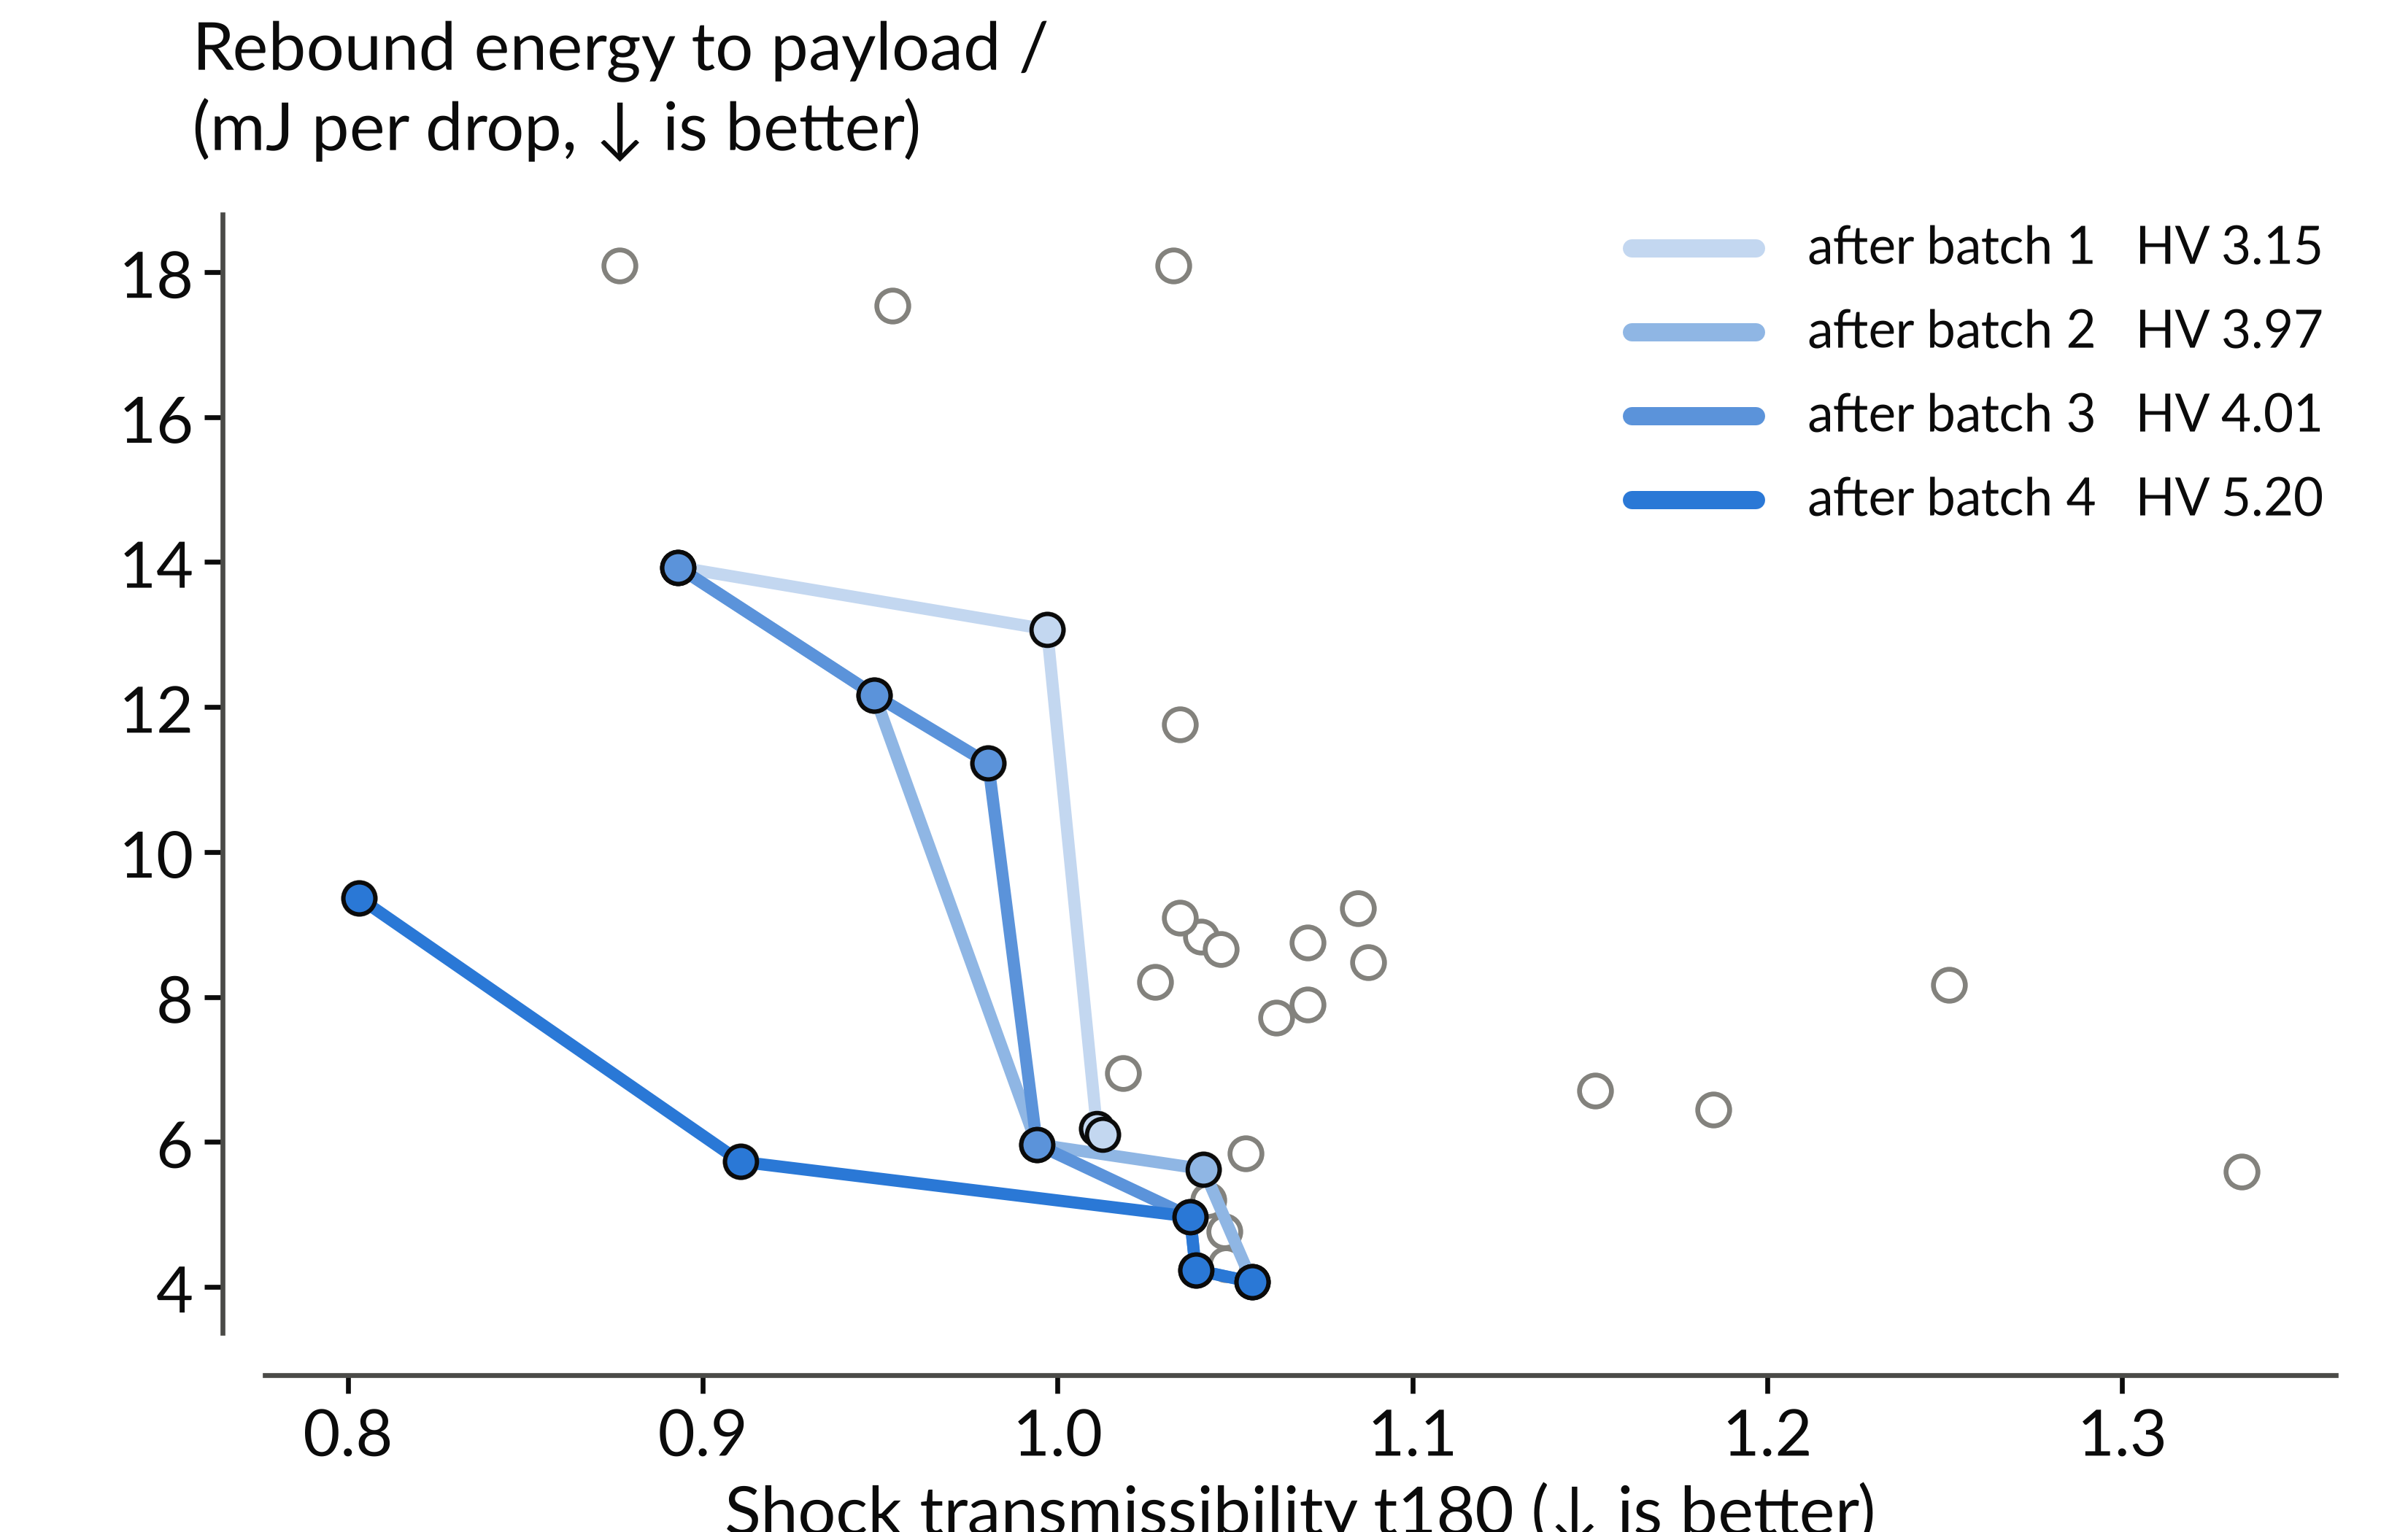
\includegraphics[width=0.85\textwidth]{../figures/bo/t3-prism-bo-front-evolution.png}
  \caption{Measured objective space and front evolution across the
    four batches. Gray circles are all measured articles at their
    stabilized means; the blue lines are the non-dominated fronts
    after each batch, with the dominated hypervolume at the
    $(1.35, \SI{15}{mJ})$ reference in the legend. Batch 2 grew the
    front on the rebound axis, batch 3 filled the knee, and batch 4
    broke the transmissibility floor. Both axes improve downward.}
  \label{fig:front-evolution}
\end{figure*}

\begin{figure*}[t]
  \centering
  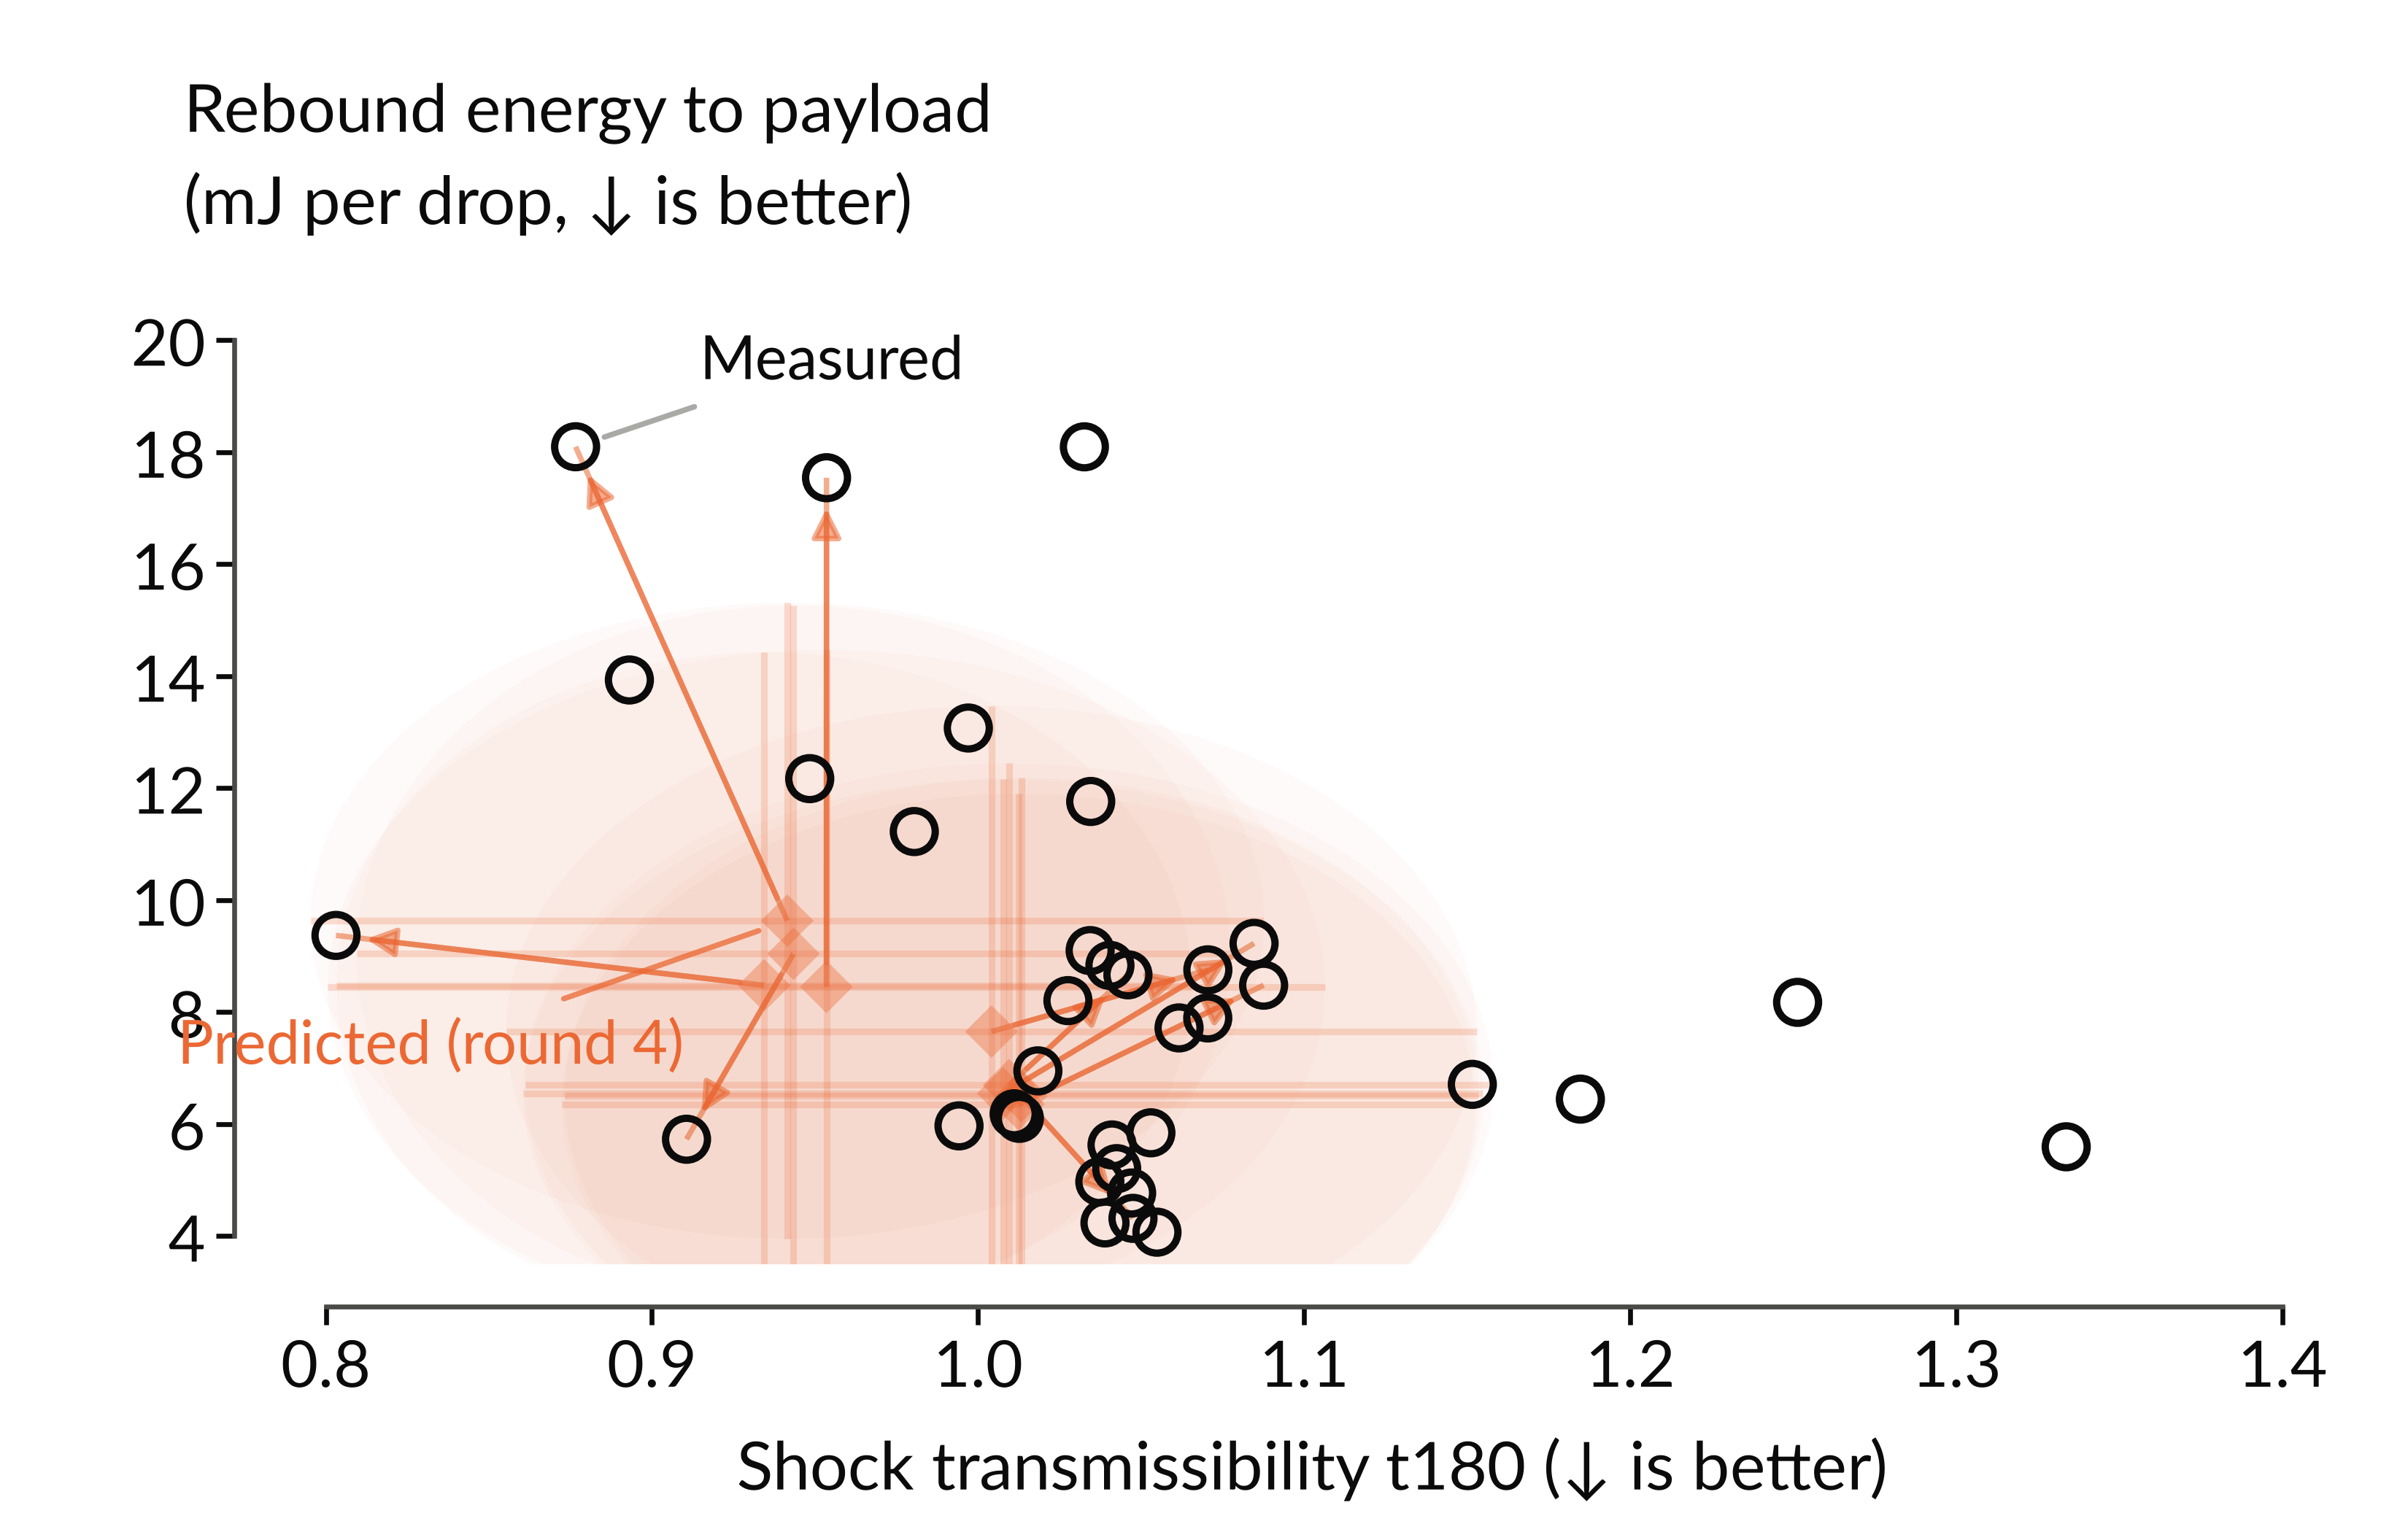
\includegraphics[width=0.85\textwidth]{../figures/bo/t3-prism-bo-round4-predicted-vs-actual.png}
  \caption{Batch-4 predictions against outcomes. Orange diamonds with
    bars are the archived posterior predictions (mean $\pm$ one
    standard deviation) for trials 37 to 45 at recommendation time;
    arrows connect each prediction to its article's measured value
    (black circles; all previously measured articles shown for
    context). The record attenuator corny7 (measured 0.803) is the
    left-most measured point. Both axes improve downward.}
  \label{fig:batch4-pred-vs-meas}
\end{figure*}

\subsection{Surrogate Audits Across the Campaign}
\label{sec:results:audits}

Each refit is audited with leave-one-out cross-validation (LOOCV;
one full NUTS refit per held-out article) and length-scale
diagnostics. Figure~\ref{fig:sensitivity} reports the seed-state
SAASBO feature importances (normalized inverse length scales, median
over the Monte Carlo draws with interquartile whiskers, over the five
design variables plus printed mass). At seven observations for six
correlated inputs these are prior-sensitive model diagnostics only:
no input separates decisively from the equal-share line, and none
supports a claim of variable relevance or ranking.

The honest headline of the cross-validation trajectory is that
held-out point accuracy \emph{declined} as the campaign grew:
$t_{180}$ LOOCV MAPE was 2.9\% with rank correlation $+0.76$ on the
seed state (8 articles, 6 model inputs), 5.4\% and $+0.60$ after
batch 2 (17 articles), and 6.2\% and $+0.19$ after batch 3 (26
articles, 12 inputs); the rebound channel reads 29.3\%, 23.6\%, and
32.2\% MAPE at the same states
(Fig.~\ref{fig:loocv}; the fold-level records are archived with the
campaign data). Three changes landed together and are confounded:
the input space doubled from 6 to 12 while the data grew only from
17 to 26, four of the six added axes carry a single value per batch
and are therefore perfectly confounded with batch, and batch 3
itself added the campaign's largest outliers. The held-out posterior
shrinks predictions toward the pooled mean, so the campaign's
defining extremes are exactly what it misses. The practical stance
this trajectory dictates, and the one the campaign took, is to treat
predicted columns as exploration bookkeeping rather than forecasts:
batch 4's value was the design family it selected and the record it
found, not its point accuracy, and its best-predicted article was
the record. Two further audit facts round out the picture. The
mass-transmissibility correlation fell from $r = 0.82$ over the
seed articles to $0.07$ over the 26 articles of batches 1 to 3, so
the constant-printed-mass projection removed the seed batch's
dominant confound. And the planned head-to-head calibration
comparison against a point-estimated single-task GP with the same
kernel has not yet been run, so no claim is made that SAASBO
outperforms it here.

\begin{figure}[t]
  \centering
  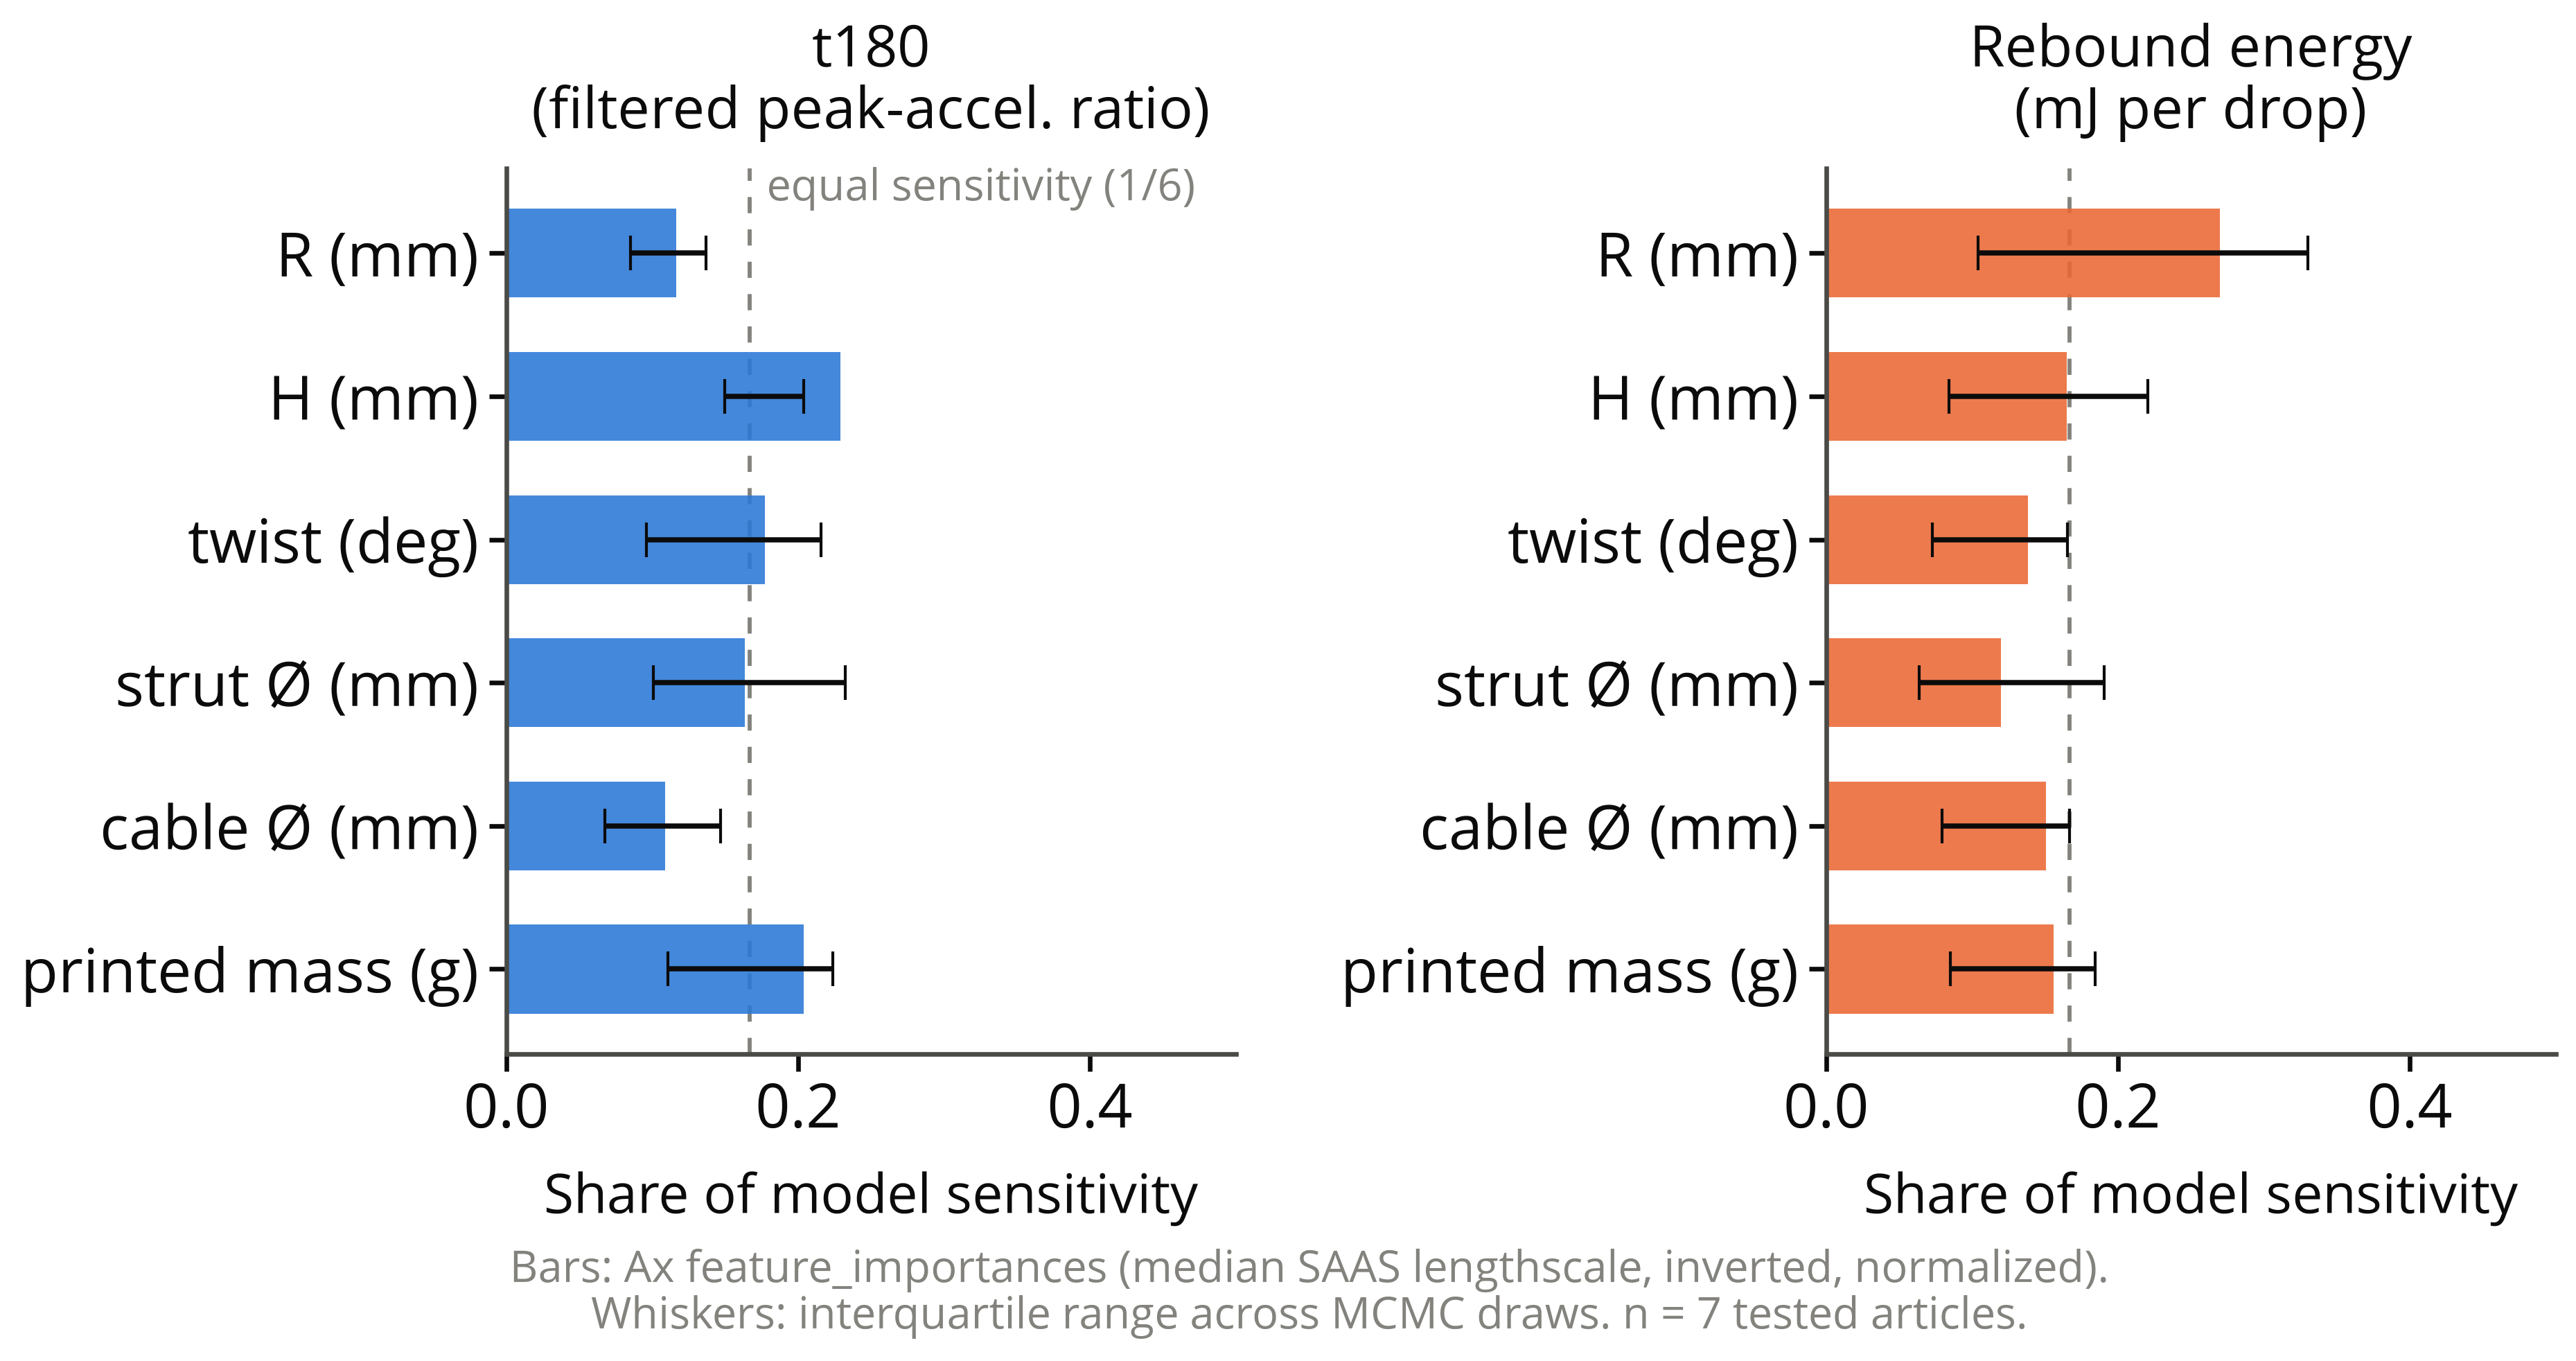
\includegraphics[width=0.92\linewidth]{../figures/bo/t3-prism-bo-round1-feature-importance.png}
  \caption{Seed-state SAASBO length-scale diagnostics per objective
    (normalized inverse length scales; median over MCMC draws,
    interquartile whiskers; inputs are the five design variables plus
    printed mass; the horizontal axis, labeled ``share of model
    sensitivity'' in the plot, is this normalized inverse-length-scale
    diagnostic). No input separates decisively from the equal-share
    line (dashed) at seven mapped articles, and these are
    prior-sensitive model diagnostics, not evidence of variable
    relevance.}
  \label{fig:sensitivity}
\end{figure}

\begin{figure}[t]
  \centering
  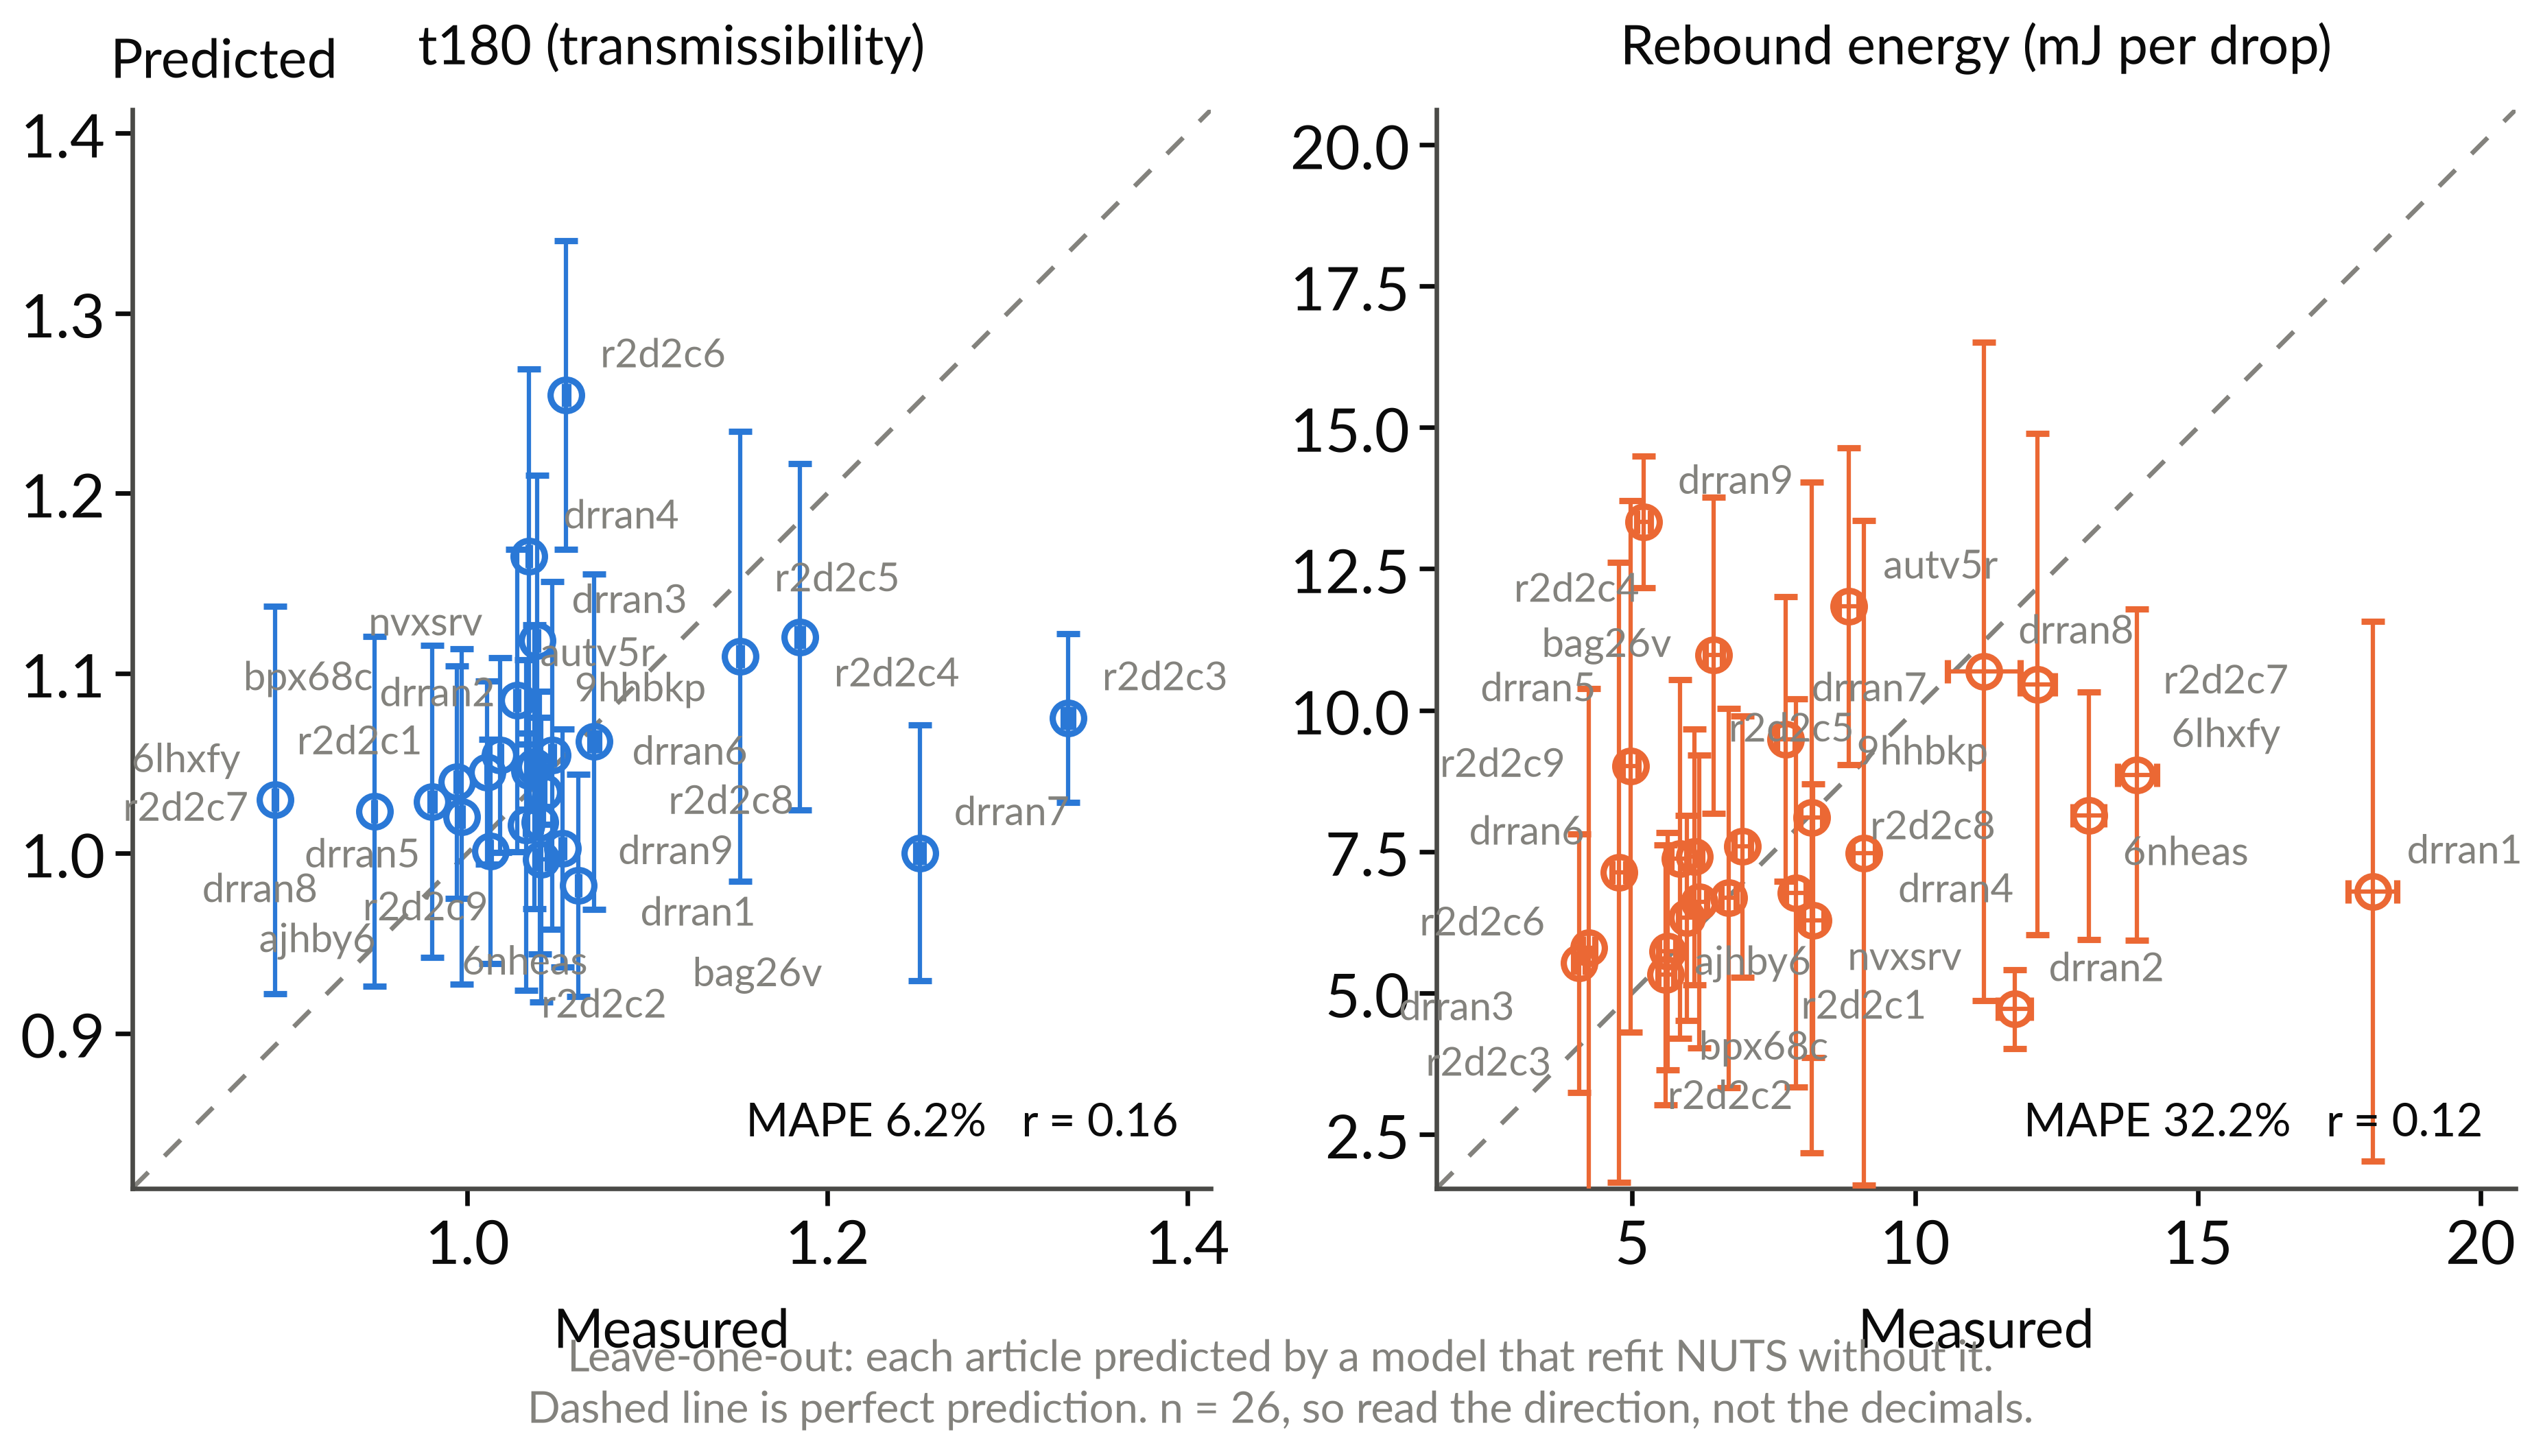
\includegraphics[width=0.92\linewidth]{../figures/bo/t3-prism-bo-round4-loocv.png}
  \caption{Leave-one-out cross-validation of the SAASBO surrogate on
    the 26 articles of batches 1 to 3 (one full NUTS refit per
    held-out article; 12 model inputs). Vertical bars are one
    posterior standard deviation of the held-out prediction;
    horizontal bars are the measured standard error as ingested. The
    dashed line is parity. The held-out posterior shrinks toward the
    pooled mean, so the extremes (r2d2c3, drran7, the seed
    attenuator) are the largest misses.}
  \label{fig:loocv}
\end{figure}

\paragraph{Studies pending} The re-seat confirmations of the batch-4
attenuators (the record article first), any batches beyond the
fourth (a fifth batch is generated and its print files staged, but
nothing from it appears here), the replicate rank-stability study of
Section~\ref{sec:methods:rankstability} (best-, mid-, and
worst-predicted in-sample designs re-printed in nominal triplicate),
the quasi-static crush campaign, and the metal-analog comparison
(Table~\ref{tab:metal-validation}) remain future work; none of their
values appear in this section.


% =============================================================================
\section{Discussion}
\label{sec:discussion}
% =============================================================================

\paragraph{What the campaign establishes} The four measured batches
settle four questions the planned-methods stage could only pose. The
end-to-end loop runs and closes, repeatedly: printed articles,
instrumented characterizations, a fitted fully Bayesian surrogate,
and three successive model-recommended batches whose own
measurements fed the next refit. The measurement distinguishes the
tested articles: the campaign $t_{180}$ means span 0.803 to 1.334,
far beyond within-session drop scatter, though
the batch-3 second pass shows that seating and print variation, not
drop scatter, set the resolution floor for any single article. The
physics is more adversarial than the cushioning intuition suggests:
at this scale and rate, most printed prisms \emph{amplify} the peak
shock reaching their top vertex (26 of 35 articles measured above
unity), which sharpened the campaign question from ``how much does
the architecture cushion'' to ``which corner of the design space
crosses into attenuation, and at what rebound cost.'' And the
batches answered that sharpened question, though not on the first
try: batch 2's forecasts were optimistic on nine of nine articles,
batch 3's best-predicted design was its worst amplifier, and batch 4
then delivered four attenuators from the wide, high-twist,
thin-cable family, led by its best-predicted design at
$t_{180} = 0.803$. The strongest attenuators still tend to carry
large rebound energies (the record article is mid-pack at
\SI{9.4}{mJ}, while the tall batch-4 family shows that near-unity
transmission with low rebound is reachable), so the front remains
genuinely two-dimensional.

\paragraph{Honest accounting of the objective stack} We
pre-registered an adversarial, data-first review of the objective
choices with an external AI referee that was required to commit to
its own objective set from the raw campaign files before reading
ours. Its findings temper the round-1 formulation and set the round-3
revision: the rebound fraction $e_{\mathrm{reb}}$ rests on a ballistic
interpretation of the second contact event that has not yet been
validated against synchronized video (a restrained-versus-unrestrained
check is scheduled); the apparent $t_{180}$-versus-rebound trade-off
is driven substantially by the single strongest attenuator (Spearman
$\rho = -0.39$, $p = 0.38$ across the reliable articles); and
per-drop standard errors are substantially smaller than the
between-article variation, and therefore understate design-level
uncertainty. The campaign's responses were physical rather than
statistical: the batch-3 plate was printed and tested twice, which
measured the same-design shift distribution directly (median
$+1.2\%$, heavy tails; Section~\ref{sec:results:batches}); the
between-seat replication rule now gates every extreme; rebound stays
a candidate constraint pending its ballistic validation; and the
constant-printed-mass projection removed the mass channel the review
flagged. We report this trajectory rather
than presenting the seed-state choices as final because the loop is
the contribution and revising objectives mid-campaign, with the
revision criteria stated in advance, is how such loops behave in
practice.

\paragraph{Mass as a confound and as a design variable} Holding
solid CAD mass constant did not hold printed grams constant: PLA
prints at partial infill while thin TPU cables print near solid, so
the seed articles span \SIrange{18.50}{22.29}{g}, and among the
mapped seed articles mass and $t_{180}$ are correlated
($r = 0.82$). Printed mass is itself induced by the geometry and is
strongly collinear with member dimensions (light articles \emph{are}
the thick-strut, thin-cable corner by construction), so the seed
observations cannot identify separate geometry and mass effects; a
post hoc mass-adjusted regression would be unstable and would
estimate a different, direct-effect quantity. The campaign's answer
was experimental design rather than adjustment: the calibrated
printed-mass model (Supplementary Information) let batches 3 and 4
compare geometries at fixed printed grams (batch mass CVs of 1.7 and
2.3\%), and the mass-transmissibility correlation across the
articles of batches 1 to 3 fell to $r = 0.07$. The confound was
broken by construction, and the mass-aware rebound objective keeps
grams penalized where they physically matter, in the energy returned
to the payload.

\paragraph{Relation to prior art, and why simulation sits outside
the loop} Relative to Pajunen
et~al.~\cite{pajunen2019design}, the present work varies the geometry
under an optimization loop rather than characterizing a single
fabrication condition; relative to Mo
et~al.~\cite{mo2023accelerated}, the loop's ground truth is physical
measurement, and no simulated number enters the objectives, the
acquisition, or candidate priority. That exclusion is a measured
decision, not an omission: an exploratory multi-engine simulation
study conducted alongside the campaign (rigid-body through
finite-element fidelities, archived in the project repository) could
not reproduce the amplification that dominates the measured record
(rigid-strut models cap the transmissibility near unity while most
printed articles exceed it), predicted design-invariant rebound
where the measurement discriminates strongly, and correlated only
weakly with the measured transmissibility. Its constant-mass
fairness constraints and its diagnosis of the seed batch's
mass-rebound confound did shape the campaign design, which is the
screening role we consider simulation to have earned here; anything
more must first demonstrate prospective predictive skill on
articles it has not seen. The measured near-unity
transmission of most seed articles also cautions against reading the
printed-tensegrity literature's attenuation results as generic: the
as-printed cells here are not pretensioned, and activating genuine
pretension in additively manufactured tensegrity (for example through
shrink-on-treatment routes) is an open direction we deliberately
scope out of the present campaign.

\paragraph{Practical considerations and path forward} TPU-PLA
interface durability under repeated impact remains open: no joint
failed during the repeated-drop measurement sessions (more than
1,400 stabilized captures across 35 articles plus the batch-3
second pass), but because
those sessions were not designed as controlled fatigue tests, the
observation does not establish interface durability, and pull-out
and fatigue characterization of the internal-anchor joint is an area
of planned follow-on work. Sensitivity to
print-process covariates (the print key logs defects, humidity, and
the mid-batch nozzle change for exactly this purpose) and transfer to
other material pairs likewise remain open. In the future we plan
the re-seat confirmations of the batch-4 attenuators, the replicate
rank-stability study of Section~\ref{sec:methods:rankstability}, the
metal-analog rank-transfer comparison of
Section~\ref{sec:methods:validation}, quasi-static testing as an
extension of the characterization
(Section~\ref{sec:methods:testing}), pretension activation, tiled
multi-cell absorbers and lattices~\citep{sabounizawadzka2024experimental},
and miniaturization to crutch-tip envelopes: long-term crutch use is
associated with substantial upper-extremity overuse injury and
ground-reaction-force impulses~\citep{requejo2005upperextremitykinetics,
rasouli2020walkingassistanceusing, manocha2021injuriesassociatedwith,
brasilbarrosdasilva2022painmappingand,
dozono2015peripheralneuropathiesin}; existing
spring-loaded~\citep{segura2007mechanicsofambulation,
zhang2011biomechanicalevaluationof} and
polymer-damped~\citep{macgillivray2016theinfluenceof} tip designs
reduce loading rate but not peak transmitted force, and recent
tensegrity crutch concepts~\citep{gu2026tensegritycrutches} and
open-source 3D-printed crutch
work~\citep{mottaghi2025opensource3dprintable} suggest a plausible
translation path, with adjacent footwear and orthotic lattice
studies~\citep{wang2025porouslatticestructure,
zhang2024pressurereducingdesignof,
janarthanan2024additivemanufacturingof} providing transferable design
heuristics.

\paragraph{Limitations} The measured evidence base is 35 articles
across four batches, but with one mechanical-response article per
design in the fit: only batch 3 has a second printed-and-tested set,
and that replication is what exposed the seating and print
sensitivity, so every single-article extreme, including the batch-4
record, is provisional until its re-seat. The drop protocol probes
one height, one impact surface, and axial loading only; the
specimens never leave the elastic regime, so crush-energy metrics
await the quasi-static campaign; per-specimen energy absorption in
joules is not recoverable from the current rig (the falling-mass and
displacement channels required for a force integral are not
instrumented); the four filament axes carry one value per batch and
are unidentified; the held-out prediction skill of the surrogate
declined as the input space grew
(Section~\ref{sec:results:audits}); one tested seed article lacks a
design mapping, one seed design's official article assignment
carries a recorded discrepancy, and two seed designs have no session
record; and all results are from a single printer, material pair,
and cell topology. The replication rule, the planned re-seat
confirmations, the replicate rank-stability study
(Section~\ref{sec:methods:rankstability}), and the metal-analog
protocol (Section~\ref{sec:methods:validation}) are the designed
responses to these limits.

% =============================================================================
\section{Conclusions}
\label{sec:conclusions}
% =============================================================================

We have presented an experiment-driven Bayesian-optimization
framework for designing multi-material 3D-printed tensegrity-inspired
energy absorbers, with TPU used in place of the traditional tension
elements and PLA members carrying compression most of the time, and
we have run it through the recommend, fabricate, measure, and update
cycle three times on physical hardware. The framework parameterizes a
$T_3$-prism family (five geometry variables, joined in batch 3 by
infill and filament process variables) under a constant-mass fairness
projection, fabricates each candidate in a single multi-material FDM
build with TPU tendons anchored inside the PLA strut ends,
characterizes every article with repeated instrumented drops (101
stabilized captures in the seed batch, about twenty thereafter), and
updates a fully Bayesian Gaussian-process
surrogate~\citep{balandat2020botorch, eriksson2021saasbo} that
recommends the next batch. Across the four measured batches (35
articles), the transmissibility spanned 0.803 to 1.334, most
articles amplified the peak shock, and the model-recommended batches
grew the dominated hypervolume 65\% over the Sobol seed front,
ending with a front whose five members are all model-chosen; the
batch-4 best-predicted design set the program record at
$t_{180} = 0.803$, ten percent below the best seed article, and
awaits its re-seat confirmation under the campaign's replication
rule. A second print-and-test pass of one batch showed that seating
and print variation, not drop-to-drop scatter, bound design-level
claims, which is the workflow lesson we consider most transferable.
The workflow is a candidate for other experimentally
evaluated architected structures whose constitutive response is
difficult to calibrate from first principles, but transfer beyond this
printer, material pair, topology, and axial impact condition remains
untested.

% =============================================================================
% Back matter
% =============================================================================
\section*{Acknowledgment} % ASME requests this exact spelling, singular.

This work was supported by the Brigham Young University Mentored
Research Grant program. The authors thank the undergraduate researchers
who carried out the multi-material printing and impact testing, and the
graduate co-mentor who supported day-to-day operations.
\todo{Confirm exact grant numbers and acknowledge any
NASA/Utah-Space-Grant-Consortium support per
acknowledgment-text guidelines.}

\section*{Funding Data}
\begin{itemize}
  \item Brigham Young University Mentored Research Grant.
\end{itemize}
\todo[inline]{Insert the MRG award number, and add the Utah NASA Space
Grant Consortium award if applicable.}

\section*{Conflict of Interest}
The authors declare no conflict of interest.

% Print the list of pending TODOs at the end -- the [disable] option
% on todonotes hides this automatically in the clean wrapper.
\listoftodos[Pending TODOs and figure/table placeholders]

% -----------------------------------------------------------------------------
% References (ASME numeric style; uses asmejour.bst)
% -----------------------------------------------------------------------------
\bibliographystyle{asmejour}
\bibliography{references}

\end{document}
